% 主文件：《近场动力学理论与数值方法》
\documentclass[UTF8, a4paper, 11pt]{ctexbook}

% 导言区：《近场动力学理论与数值方法》

% ---------- 页面设置 ----------
\usepackage[a4paper, top=2.5cm, bottom=2.5cm, left=3cm, right=2.5cm]{geometry}

% ---------- 常用宏包 ----------
\usepackage{amsmath}
\usepackage{amssymb}
\usepackage{amsthm}
\usepackage{graphicx}
\usepackage[font=small,labelsep=quad]{caption}
\graphicspath{{figures/}}
\usepackage{booktabs}
\usepackage{xcolor}
\usepackage{enumitem}
\usepackage{titlesec}
\usepackage{fancyhdr}
\usepackage{tikz}
\usepackage{listings}
\usepackage[colorlinks=true, linkcolor=blue, citecolor=blue, urlcolor=blue]{hyperref}

% ---------- 章节标题样式 ----------
\ctexset{
  chapter = {
    format = \centering\Huge\bfseries,
    name   = {第,章},
    number = \arabic{chapter},
  },
  section = {
    format = \Large\bfseries,
  },
  subsection = {
    format = \large\bfseries,
  },
}
% ---------- 目录深度设置 ----------
\setcounter{tocdepth}{1}
% Patch \addcontentsline to respect tocdepth at write time
% (titlesec writes all levels to .toc by design; this patch filters at write time)
\makeatletter
\def\pd@toclevel@section{1}
\def\pd@toclevel@subsection{2}
\def\pd@toclevel@subsubsection{3}
\def\pd@toclevel@paragraph{4}
\def\pd@toclevel@subparagraph{5}
\let\pd@addcontentsline@orig\addcontentsline
\renewcommand{\addcontentsline}[3]{%
  \def\pd@tmpa{#1}%
  \def\pd@tmpb{toc}%
  \ifx\pd@tmpa\pd@tmpb
    \@ifundefined{pd@toclevel@#2}{%
      \pd@addcontentsline@orig{#1}{#2}{#3}%
    }{%
      \ifnum\@nameuse{pd@toclevel@#2}>\c@tocdepth\relax\else
        \pd@addcontentsline@orig{#1}{#2}{#3}%
      \fi
    }%
  \else
    \pd@addcontentsline@orig{#1}{#2}{#3}%
  \fi
}
\makeatother
\captionsetup[figure]{name=图,labelsep=quad}
\captionsetup[table]{name=表,labelsep=quad}

% ---------- 页眉页脚 ----------
\pagestyle{fancy}
\fancyhf{}
\fancyhead[C]{\leftmark}
\fancyfoot[C]{\thepage}
\setlength{\headheight}{13.6pt}

% ---------- 定理环境 ----------
\newtheorem{theorem}{定理}[chapter]
\newtheorem{definition}{定义}[chapter]
\newtheorem{lemma}{引理}[chapter]
\newtheorem{remark}{注记}[chapter]
\newtheorem{example}{例}[chapter]

% ---------- 代码环境 ----------
\lstset{
  basicstyle       = \ttfamily\small,
  keywordstyle     = \color{blue},
  commentstyle     = \color{gray},
  stringstyle      = \color{red},
  frame            = single,
  breaklines       = true,
  numbers          = left,
  numberstyle      = \tiny\color{gray},
  showstringspaces = false,
}


\begin{document}

\frontmatter
% 封面
\begin{titlepage}
  \centering
  \vspace*{4cm}
  {\Huge\bfseries 近场动力学理论与数值方法\par}
  \vspace{2cm}
  {\Large 刘黎旺，傅帅旸\par}
  \vfill
\end{titlepage}

% 前言
\chapter{前言}

\tableofcontents
% 符号表
\chapter{符号表}


\mainmatter
% 第1章 绪论
\chapter{绪论}

\leavevmode\usetikzlibrary{arrows.meta, positioning, calc, decorations.pathmorphing, shapes.geometric}

固体力学的核心任务之一，是描述材料从连续变形到最终破坏的全过程。断裂与损伤是工程结构失效的最常见形式，然而经典连续介质力学在处理这类强不连续问题时遭遇了深层次的困难。本章首先回顾经典连续介质力学的基本假设及其在断裂问题中的根本局限（1.1节），进而追溯非局部理论的发展脉络（1.2节），引出近场动力学的诞生（1.3节），阐明其核心思想与基本特征（1.4节），并按研究方向系统梳理其发展历程与研究现状（1.5节），最后介绍本书的结构与阅读建议（1.6节）。本章的目的不在于给出严格的数学推导，而在于回答两个基本问题：为什么需要近场动力学，以及近场动力学是什么。严格的数学框架将在第2章建立，近场动力学与经典连续介质力学的关系将在第3章详细分析。

\section{经典连续介质力学的局限与挑战}

经典连续介质力学（classical continuum mechanics，简称 CCM）自 18 世纪以来一直是固体力学与工程分析的基石。它以两个基本假设为前提。一是连续性假设，认为材料占据的空间区域可以逐点定义密度、位移、应力等场量。二是局部作用假设，认为材料点只与其无穷小邻域内的物质发生相互作用，其力学状态完全由该点处的变形梯度决定。在这两个假设之下，线动量平衡可以写成含空间导数的偏微分方程
\[
  \nabla\cdot\boldsymbol{\sigma}+\mathbf{b}=\rho\ddot{\mathbf{u}}
\]
其中 $\boldsymbol{\sigma}$ 为 Cauchy 应力张量，$\mathbf{b}$ 为体力密度，$\mathbf{u}$ 为位移场，$\rho$ 为质量密度。应力与应变通过本构方程相联系，工程问题大多借助有限元等数值方法求解这一局部微分方程系统。这套框架在结构分析中取得了巨大成功，但它的两个基本假设恰恰构成其处理断裂问题时困境的根源 \cite{Silling2000}。

第一个困难来自位移场的不连续。断裂的本质是在材料中形成位移不连续面，即裂纹面。在不连续面上，位移对空间坐标的偏导数没有定义，而经典理论恰恰用这些偏导数来表示相邻材料点之间的相对位移与相互作用力。正如 Silling 所指出的 \cite{Silling2000}，固体力学中诸多基本问题恰恰以这种自发形成的不连续为核心，而连续介质力学的数学框架在某种程度上并不适合描述这类问题，因为沿不连续处所需的空间偏导数按定义不存在。传统的处理方式是把裂纹作为额外的人为对象引入：预先假定裂纹位置，将其表面设为自由边界，再附加专门的断裂准则决定其扩展。这种先假设、再验证的范式在裂纹路径未知、多裂纹相互作用或裂纹分叉的情形下变得极为困难。

第二个困难是裂纹尖端场的奇异性。对线弹性材料中的平面裂纹，Irwin 的分析表明 \cite{Irwin1957}，裂纹尖端附近的应力场具有
\[
  \sigma_{ij}\sim\frac{K_I}{\sqrt{2\pi r}}\qquad(r\to 0)
\]
的形式，其中 $K_I$ 为 I 型应力强度因子，$r$ 为距裂尖的距离。当 $r$ 趋于零时，应力趋于无穷大，这在物理上不可接受。这一奇异性意味着经典弹性理论无法给出裂尖处的真实应力状态，必须借助应力强度因子或能量释放率等概念加以回避。Griffith 最早从能量角度建立了断裂准则 \cite{Griffith1921}，认为当裂纹扩展所释放的弹性能足以支付新表面所需的表面能时，裂纹发生失稳扩展。该准则给出的临界应力为
\[
  \sigma_c=\sqrt{\frac{2E\gamma}{\pi a}}
\]
其中 $E$ 为弹性模量，$\gamma$ 为表面能密度，$a$ 为裂纹半长。这一公式同时暴露出 Griffith 准则的根本局限。当裂纹尺寸 $a$ 趋于零时，临界应力趋于无穷大，因此该准则无法回答无初始裂纹的完整构件在多大载荷下萌生裂纹这一基本问题。此外，它只能判定裂纹在什么条件下扩展，既不能预测扩展方向，也不能处理裂纹分叉、跳跃以及多裂纹之间的相互作用。Irwin 的应力强度因子方法 \cite{Irwin1957} 在工程上十分有效，但同样需要预知裂纹的几何与位置，本质上属于裂纹扩展准则而非裂纹萌生理论。裂纹尖端应力场的形式如图\ref{fig:crack-singularity}所示：当距裂纹尖端距离 $r \to 0$ 时，应力按 $r^{-1/2}$ 发散，这正是经典弹性理论预测的应力奇异性——裂纹尖端应力趋于无穷，在物理上并不合理。

\begin{figure}[htbp]
  \centering
  \begin{tikzpicture}[scale=0.9]
    % 左：含裂纹平板
    \draw[thick] (-3,1.5) rectangle (3,-1.5);
    \draw[ultra thick] (-1.5,0) -- (1.5,0);
    \draw[-Stealth, thick] (-2,2) -- (-2,1.5);
    \draw[-Stealth, thick] (2,2) -- (2,1.5);
    \draw[-Stealth, thick] (-2,-2) -- (-2,-1.5);
    \draw[-Stealth, thick] (2,-2) -- (2,-1.5);
    \node at (-2,2.3) {$\sigma$};
    \node at (2,2.3) {$\sigma$};
    \node[below] at (0,-1.8) {(a) 含裂纹平板};
    % 右：σ-r曲线
    \begin{scope}[xshift=6cm]
      \draw[-Stealth] (0,0) -- (3.5,0) node[right] {$r$};
      \draw[-Stealth] (0,-1.5) -- (0,2.5) node[above] {$\sigma$};
      \draw[dashed] (0,0) -- (0,2.2);
      \draw[thick, blue, domain=0.3:3, samples=50] plot (\x, {1.2/sqrt(\x)});
      \node[blue, right] at (1.5,1.0) {$\sigma \sim r^{-1/2}$};
      \node[red, left] at (0,2.0) {$\infty$};
      \node[below] at (1.5,-1.8) {(b) 裂尖应力奇异性};
    \end{scope}
  \end{tikzpicture}
  \caption{裂纹尖端应力奇异性示意，经典弹性理论预测裂尖处应力趋于无穷大}
  \label{fig:crack-singularity}
\end{figure}

第三个困难来自材料软化导致的数学不适定与网格依赖。1958 年，Kachanov 以连续损伤力学开创了对材料劣化的连续描述 \cite{Kachanov1958}，通过损伤变量刻画刚度的退化。然而当损伤本构包含应变软化段时，边值问题将失去适定性。Ba\v{z}ant 与 Belytschko 以一维应变软化杆为例给出了精确解 \cite{BazantBelytschko1985}，证明变形局部化在数学上收敛于零测度集合，损伤带的宽度随网格细化而趋于零，能量耗散也随之趋于零，数值结果对网格产生灾难性的依赖。换言之，损伤被数值压缩进零体积，完全损伤区（completely damaged zone，简称 CDZ）失去物理意义，这正是连续损伤力学在断裂预测中屡屡失效的根源。

为恢复适定性，研究者提出了多种正则化手段。Pijaudier-Cabot 与 Ba\v{z}ant 引入非局部损伤模型 \cite{PijaudierCabotBazant1987}，以特征长度加权的积分平均替代点值；Peerlings 等发展梯度增强损伤模型 \cite{Peerlings1996}，在本构中引入应变的高阶梯度；此外还有微极连续体等含独立转动自由度的理论（其历史脉络见 1.2 节 \cite{Cosserat1909}）。这些方法都引入了内部长度尺度，在一定程度上缓解了网格依赖，但它们大多仍然建立在偏微分方程与应力张量的框架之内，在裂纹萌生、分叉与汇合等强不连续问题面前仍然力不从心，且正则化参数的选取缺乏统一的物理依据。

上述分析表明，断裂问题的困难并非某个细节处理不当，而是源于经典理论以微分描述相互作用这一基本架构。要使不连续的产生与演化成为方程的自然结果，需要一种在数学上自洽、在构造上不以连续位移场为前提的理论。这正是近场动力学试图提供的。图\ref{fig:pd-paradigm}对比了经典连续介质力学、离散方法与近场动力学三种范式对材料点相互作用的不同描述方式。

\begin{figure}[htbp]
  \centering
  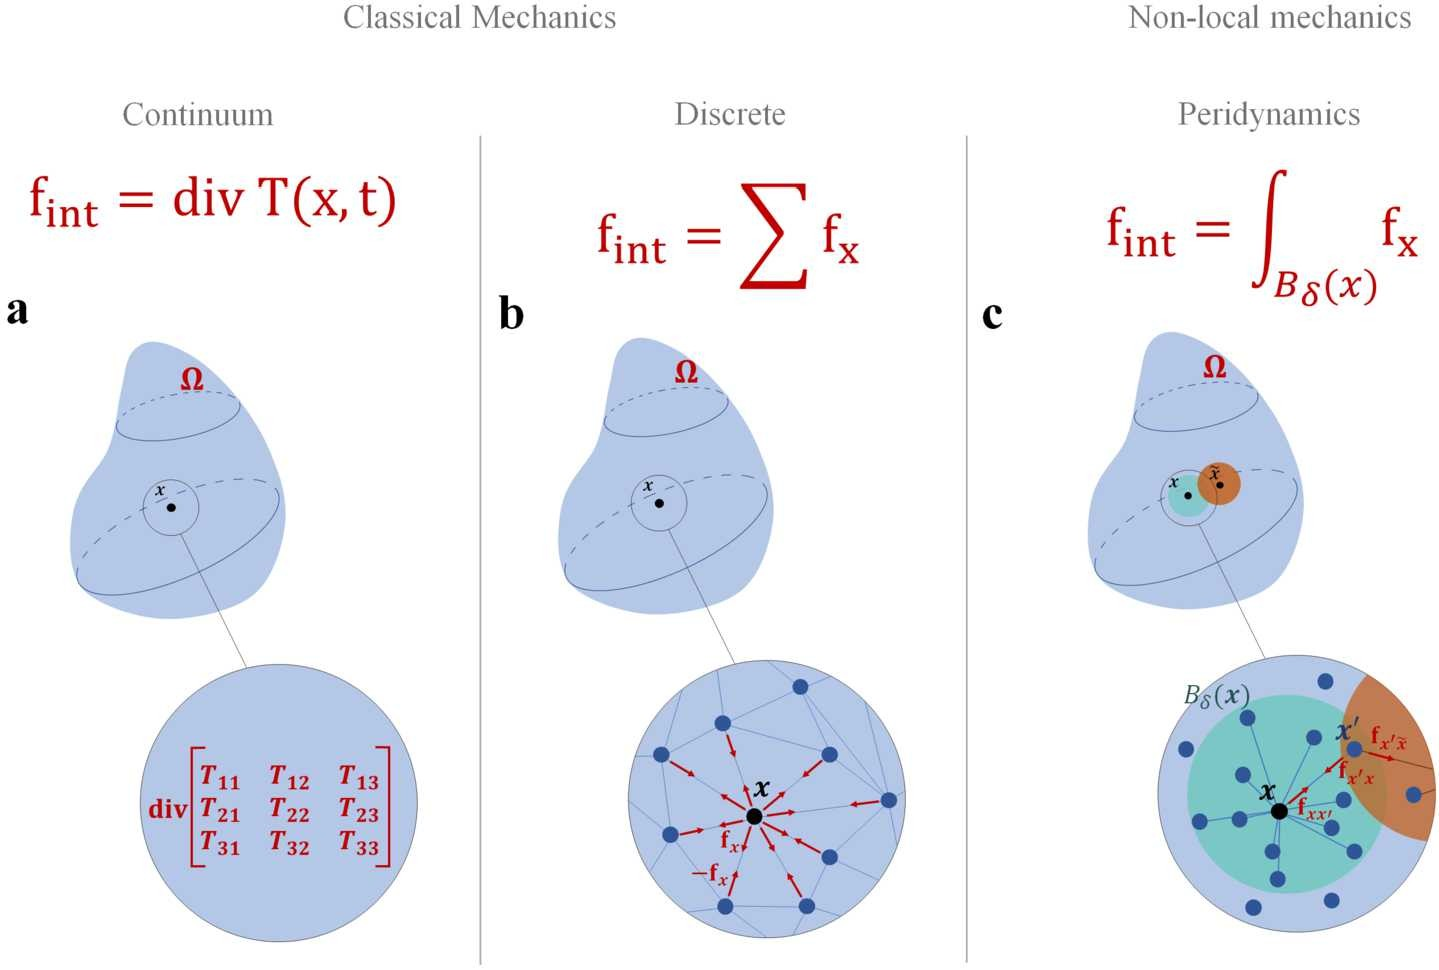
\includegraphics[width=0.85\textwidth]{dimola2022_fig1.png}
  \caption{经典连续介质力学、离散方法与近场动力学对材料点相互作用的描述范式示意（图片来源\cite{Dimola2022}）}
  \label{fig:pd-paradigm}
\end{figure}

\section{非局部理论的起源与发展}

非局部思想在力学中由来已久，其源头可以追溯到 19 世纪。1887 年，Voigt 在晶体弹性的研究中引入比经典 Cauchy 理论更丰富的自由度描述 \cite{Voigt1887}。1909 年，Cosserat 兄弟在《可变形体的理论》（Th\'{e}orie des corps d\'{e}formables）中系统建立了微极连续体理论 \cite{Cosserat1909}，赋予材料点独立的转动自由度，使应力张量不再对称，并引入偶应力。这些工作在当时的框架内属于少数派，却为后来的微结构与梯度理论埋下了伏笔。

现代非局部弹性理论的确立以 Kr\"{o}ner 1967 年的工作为标志 \cite{Kroner1967}。Kr\"{o}ner 提出了第一个长程内聚力弹性模型，材料点之间的相互作用不再局限于无穷小邻域，而是延伸到有限距离。此后，Eringen 及其合作者将这一思想发展为系统的理论体系。Eringen 与 Edelen 于 1972 年建立了非局部弹性的公理化框架 \cite{EringenEdelen1972}，同年 Eringen 给出线性非局部弹性理论，并研究了平面波的色散 \cite{Eringen1972}。在该框架中，应力被表述为整个定义域上应变的泛函，典型形式为
\[
  \sigma_{ij}(\mathbf{x})=\int_V \alpha(|\mathbf{x}'-\mathbf{x}|)\,C_{ijkl}\,\varepsilon_{kl}(\mathbf{x}')\,dV'
\]
其中 $\alpha$ 为随距离衰减的衰减函数（attenuation function），即核函数，它刻画了长程相互作用的强度随距离的变化。当核函数退化为 Dirac 函数时，上式回到经典局部本构关系，可见经典理论是非局部理论的一个极限情形。1983 年，Eringen 进一步指出 \cite{Eringen1983}，若将积分核取为某个微分算子的 Green 函数，则上述积分型本构可以等价地写成微分形式，例如
\[
  (1-l^2\nabla^2)\sigma_{ij}=C_{ijkl}\varepsilon_{kl}
\]
其中 $l$ 为材料内禀长度尺度（intrinsic length scale），即刻画微结构对力学行为影响范围的特征长度。经典本构中不含任何长度参数，应力仅取决于当前点的应变；内禀长度的引入使本构关系能够感知有限空间范围内的非局部效应，其值通常与晶格常数、晶粒尺寸等微结构尺度相联系。这一微分形式的非局部理论在纳米力学中获得了广泛应用。

积分核与长度尺度的引入，使非局部理论能够描述经典理论无法刻画的尺度效应。原子晶格的色散关系对波数的依赖，在非局部弹性中通过核函数的 Fourier 变换自然浮现，而经典弹性理论只能描述长波极限行为。非局部理论还在位错芯结构、表面效应与纳米结构力学中得到了应用，其长度尺度 $l$ 通常与材料的微结构特征尺度相当。但核函数的具体形式及其参数缺乏来自底层物理的直接约束，往往需要借助实验或原子模拟加以标定，这成为非局部理论走向定量预测的一个障碍。

另一条平行的路线是梯度理论。Mindlin 于 1964 年建立了含微结构的线弹性理论 \cite{Mindlin1964}，将应变能密度写为应变及其梯度乃至更高阶导数的函数；Aifantis 等则将梯度项引入塑性本构，用于描述应变局域化 \cite{Aifantis1992}。梯度理论可以看作核函数具有特殊形式的非局部理论，其共同特征是以长度尺度对高阶导数进行正则化。

非局部理论在断裂问题中取得了一个标志性成果。Eringen、Speziale 与 Kim 于 1977 年用非局部弹性求解了 Griffith 裂纹问题 \cite{Eringen1977}，发现裂纹尖端处的应力保持有限，经典的 $r^{-1/2}$ 奇异性被消除，从而可以基于最大应力假设建立断裂准则。这一结果令人鼓舞，表明非局部化确实能够从本质上改变裂尖场的结构，也为后来近场动力学中键的临界伸长率准则提供了思想上的先声。

然而，非局部理论仍然存在两个根本局限。其一，它依然以应力张量和广义的偏微分方程为基本工具，微分形式的近似虽然便于求解，却再次把空间导数置于核心位置，只是在大尺度上软化了奇异性，而非消灭了它。其二，积分型非局部本构在位移场连续光滑时行之有效，一旦裂纹萌生、位移场出现真实的不连续，积分核跨越不连续面的合理性就需要重新审视。换言之，非局部理论仍然把不连续视为需要额外处理的例外情形。近场动力学正是在这一历史背景下，对固体力学基本方程所做的一次更为彻底的重新表述：不是修正经典理论，而是另起炉灶，以不连续量为天然合法的对象。

\section{近场动力学的诞生}

20 世纪 90 年代末，美国 Sandia 国家实验室承担核武器库存管理计划（Stockpile Stewardship Program）中的数值模拟任务。该计划要求在不进行地下核试验的条件下，依靠高置信度数值模拟预测武器部件在老化、冲击与复杂载荷下的行为，其中金属与复合材料部件的断裂与破碎模拟是关键环节。传统有限元方法在裂纹萌生与动态分叉问题上的固有困难，促使 Silling 思考一个更根本的问题：能否构造一种从一开始就不依赖空间导数的固体力学表述。

2000 年，Silling 在 \textit{Journal of the Mechanics and Physics of Solids} 上发表了创始论文《Reformulation of elasticity theory for discontinuities and long-range forces》\cite{Silling2000}。该文的核心思想极为简洁：用积分代替微分来计算材料点所受的力。近场动力学的运动方程不涉及任何位移的空间导数，因此在不连续点或不连续面上同样有效，裂纹可以沿任意方向自然萌生与扩展，而不需要预设裂纹路径。Silling 将这种表述命名为 peridynamic，取自希腊语词根 peri（近）与 dynamis（力），强调其本质是近程力作用下的动力学理论。论文给出了键基（bond-based）理论的第一个具体模型，即原型微弹性脆性（prototype microelastic brittle，简称 PMB）模型，其中键力与键的伸长成正比，键伸长超过临界值时键发生不可逆断裂。文中推导了线性化理论的波色散关系，证明当所关注的波长远大于近场范围时，色散关系与经典线弹性理论一致，即近场动力学在大尺度极限下给出与经典理论相符的行为。同时，经典意义上的应变能密度可以从近场动力学的成对势函数导出，这为两类理论的衔接提供了依据。Silling 特别强调，近场动力学是一种连续介质理论，无需模拟单个原子，也不必知道真实而物理正确的原子间势，这使它区别于分子动力学（molecular dynamics，简称 MD）。

2005 年，Silling 与 Askari 提出了键基理论的数值实现方案，即 EMU 方法 \cite{SillingAskari2005}。该方法采用均匀网格离散，以中点求积近似近场积分，形式简单、易于并行，并成功模拟了动态裂纹扩展，开启了近场动力学数值计算的时代。键基理论有一个明显的局限：其本构基于成对中心力，对于三维各向同性材料，这迫使泊松比固定为 $1/4$ \cite{SillingAskari2005}，无法描述绝大多数工程材料。为突破这一限制，Silling 与 Epton、Weckner、Xu、Askari 于 2007 年提出了态基（state-based）理论 \cite{Silling2007}，引入变形态与力态（state）的概念，将键的力推广为依赖于整个近场域内变形构型的向量值函数。态基理论分为常规态基（ordinary state-based）与非常规态基（non-ordinary state-based）两类：前者中键力仍沿键的方向作用，但强度可依键而异；后者允许键力偏离键的方向。特别地，非常规态基理论中的本构对应（constitutive correspondence）机制可以把经典连续介质力学的本构模型直接嵌入近场动力学框架，从而在非局部积分框架内复用成熟的经典本构。态基理论的提出使近场动力学从单一材料模型成长为具有完整理论体系的固体力学分支。2010 年，Silling 与 Lehoucq 在 \textit{Advances in Applied Mechanics} 上发表了长篇综述 \cite{SillingLehoucq2010}，系统建立了近场动力学的守恒律、本构与线性化理论，标志着该理论框架的成熟。

\begin{remark}
  从方法论上看，近场动力学与 1.1 节讨论的各种正则化方法有本质区别。正则化方法是在经典框架内修补奇异性，而近场动力学是重新表述基本方程，使不连续从一开始就无须特殊处理。理解这一区别，是理解全书后续内容的关键。
\end{remark}

\section{近场动力学的核心思想与基本特征}

近场动力学的出发点是重新思考材料点如何感受周围环境。在经典理论中，材料点只与其无穷小邻域相互作用；在近场动力学中，材料点 $\mathbf{x}$ 与其近场范围（horizon）$\delta$ 之内的所有材料点 $\mathbf{x}'$ 相互作用，该相互作用由对力函数（pairwise force function）$\mathbf{f}$ 描述。运动方程为
\[
  \rho(\mathbf{x})\ddot{\mathbf{u}}(\mathbf{x},t)=\int_{H_{\mathbf{x}}}\mathbf{f}\big(\mathbf{u}(\mathbf{x}',t)-\mathbf{u}(\mathbf{x},t),\mathbf{x}'-\mathbf{x}\big)\,dV_{\mathbf{x}'}+\mathbf{b}(\mathbf{x},t)
\]
其中 $H_{\mathbf{x}}$ 表示以 $\mathbf{x}$ 为中心、$\delta$ 为半径的球邻域，称为近场域（示意图见图\ref{fig:horizon-bond}）。与经典运动方程相比，上式唯一的区别在于以积分取代了应力的散度，但这一区别是本质性的：方程中不再出现任何空间导数。

\begin{figure}[htbp]
  \centering
  \begin{tikzpicture}[scale=1.2]
    % horizon
    \draw[dashed, thick] (0,0) circle (2);
    \node[above right] at (1.4,1.4) {$\delta$};
    % 中心点
    \filldraw (0,0) circle (2pt) node[below left] {$\mathbf{x}$};
    % 邻点与键
    \filldraw (1.5,0.8) circle (2pt) node[above right] {$\mathbf{x}'$};
    \draw[thick] (0,0) -- (1.5,0.8);
    \filldraw (-1.2,1.0) circle (2pt);
    \draw[thick] (0,0) -- (-1.2,1.0);
    \filldraw (0.5,-1.5) circle (2pt);
    \draw[thick] (0,0) -- (0.5,-1.5);
    \filldraw (-1.6,-0.5) circle (2pt);
    \draw[thick] (0,0) -- (-1.6,-0.5);
    % 标注 ξ 和 ξ+η
    \node[above] at (0.75,0.4) {$\boldsymbol{\xi}$};
    % 变形后位置
    \draw[dashed, thick, red] (0,0) -- (2.0,1.2);
    \filldraw[red] (2.0,1.2) circle (2pt);
    \node[red, above right] at (2.0,1.2) {$\mathbf{x}'+\boldsymbol{\eta}$};
    \node[red, above] at (1.0,0.6) {$\boldsymbol{\xi}+\boldsymbol{\eta}$};
    % horizon标签
    \node[above] at (0,2.2) {$H_{\mathbf{x}}$};
  \end{tikzpicture}
  \caption{近场范围与键的示意图，材料点 $\mathbf{x}$ 与其 horizon $H_{\mathbf{x}}$ 内所有点通过键相互作用}
  \label{fig:horizon-bond}
\end{figure}

图\ref{fig:horizon-bond}展示了近场范围与键的基本几何关系。近场范围 $\delta$ 的物理含义是材料点间相互作用的特征距离。当 $\delta$ 趋于零时，相互作用退化为无穷小邻域内的局部作用，近场动力学方程在形式上回到经典理论 \cite{SillingLehoucq2008}，因此经典连续介质力学可以看作近场动力学在零近场范围极限下的特例。$\delta$ 也常与材料的微结构尺度相联系：对于多晶金属可取为晶粒尺寸的量级，对于混凝土可取为骨料尺寸的量级。实际应用中 $\delta$ 的选取还需兼顾数值收敛性，通常要求近场域内包含足够多的物质点 \cite{Bobaru2009,BobaruHu2012}。

键（bond）是近场动力学的基本相互作用单元。连接 $\mathbf{x}$ 与 $\mathbf{x}'$ 的键在参考构型中的方向矢量记为 $\boldsymbol{\xi}=\mathbf{x}'-\mathbf{x}$，变形后的相对位移记为 $\boldsymbol{\eta}=\mathbf{u}(\mathbf{x}',t)-\mathbf{u}(\mathbf{x},t)$，键的伸长（stretch）定义为
\[
  s=\frac{|\boldsymbol{\xi}+\boldsymbol{\eta}|-|\boldsymbol{\xi}|}{|\boldsymbol{\xi}|}
\]
本构关系通过对力函数 $\mathbf{f}$ 描述。对线弹性微弹性材料，在小变形下对力函数可线性化为
\[
  \mathbf{f}(\boldsymbol{\eta},\boldsymbol{\xi})\approx \mathbf{C}(\boldsymbol{\xi})\,\boldsymbol{\eta}
\]
其中 $\mathbf{C}(\boldsymbol{\xi})$ 称为微观模量（micromodulus）函数，它描述了键的刚度随键长与方向的分布，其具体形式可通过令近场动力学的应变能密度在均匀变形下与经典应变能密度一致来确定 \cite{Silling2000,Silling2010}。

近场动力学与经典理论的关系值得进一步说明。一方面，线性化后的近场动力学在大尺度行为上与经典线弹性理论一致 \cite{Silling2000,Silling2010}，这是它可以作为经典理论推广的根本原因。另一方面，两者在小尺度行为上存在差异，近场动力学具有固有的非线性色散特性，波速依赖波数，这一差异在冲击与高频波问题中不可忽略 \cite{SillingLehoucq2010}。此外，给定一个经典材料，可以构造出多个近场动力学材料在均匀变形下与其等价，即一个经典材料对应多个近场动力学材料，因此从经典参数到微观模量的映射并不唯一，需要额外的约定。

近场动力学最突出的能力是裂纹的自发萌生与扩展（autonomous crack propagation）。裂纹在近场动力学中不是被预先定义的对象，而是键断裂的自然结果：当某个键的伸长超过临界值时，该键永久失效，众多键的失效累积便构成裂纹面。这一机制使裂纹的萌生 \cite{SillingWeckner2010}、扩展与分叉 \cite{HaBobaru2010} 以及多裂纹的相互作用都可以在同一套方程下自动产生，无需任何外部断裂准则。裂纹的萌生、扩展与路径选择全部内生于运动方程与本构模型，这正是近场动力学与经典断裂力学在方法论上的根本分别。图\ref{fig:bond-breakage}示意了键网络从完整到逐步断裂并最终形成裂纹面的过程：断裂并非一次性地插入裂纹，而是大量键在不同时刻独立失效的渐进累积——这一“自下而上”的断裂机制使得裂纹的萌生、扩展与分叉都成为解的组成部分，无需任何外部准则介入。

\begin{figure}[htbp]
  \centering
  \begin{tikzpicture}[scale=0.7]
    % (a) 完整键网络
    \begin{scope}
      \foreach \x in {0,1,2,3} {
          \foreach \y in {0,1,2} {
              \filldraw (\x,\y) circle (3pt);
            }
        }
      \foreach \x in {0,1,2} {
          \foreach \y in {0,1,2} {
              \draw[thin] (\x,\y) -- (\x+1,\y);
              \draw[thin] (\x,\y) -- (\x,\y+1);
              \draw[thin] (\x,\y) -- (\x+1,\y+1);
            }
        }
      \node[below] at (1.5,-0.5) {(a) 完整键网络};
    \end{scope}
    % (b) 部分键断裂
    \begin{scope}[xshift=5cm]
      \foreach \x in {0,1,2,3} {
          \foreach \y in {0,1,2} {
              \filldraw (\x,\y) circle (3pt);
            }
        }
      \foreach \x in {0,1,2} {
          \foreach \y in {0,1,2} {
              \draw[thin] (\x,\y) -- (\x+1,\y);
              \draw[thin] (\x,\y) -- (\x,\y+1);
              \draw[thin] (\x,\y) -- (\x+1,\y+1);
            }
        }
      % 断裂的键
      \draw[red, ultra thick] (1,1) -- (2,1);
      \node[red] at (1.5,1.3) {$\times$};
      \draw[red, ultra thick] (0,1) -- (1,1);
      \node[red] at (0.5,1.3) {$\times$};
      \draw[red, ultra thick] (1,0) -- (2,1);
      \node[red] at (1.3,0.3) {$\times$};
      \node[below] at (1.5,-0.5) {(b) 键逐步断裂};
    \end{scope}
    % (c) 裂纹面形成
    \begin{scope}[xshift=10cm]
      \foreach \x in {0,1,2,3} {
          \foreach \y in {0,1,2} {
              \filldraw (\x,\y) circle (3pt);
            }
        }
      \foreach \x in {0,1,2} {
          \foreach \y in {0,1,2} {
              \draw[thin] (\x,\y) -- (\x+1,\y);
              \draw[thin] (\x,\y) -- (\x,\y+1);
              \draw[thin] (\x,\y) -- (\x+1,\y+1);
            }
        }
      % 裂纹面
      \draw[red, ultra thick] (0,1) -- (3,1);
      \node[below] at (1.5,-0.5) {(c) 裂纹面形成};
    \end{scope}
  \end{tikzpicture}
  \caption{键断裂与裂纹形成过程，裂纹是键失效的自然累积结果，无需预设裂纹路径}
  \label{fig:bond-breakage}
\end{figure}

将近场动力学与分子动力学（MD）类比是有益的。两者都通过求和（积分）计算粒子（材料点）所受的力，运动方程的形式相近。但近场动力学是连续介质理论，不需要知道原子间势；其材料具有参考构型的记忆，本构关系基于变形而非势能面，因此可以描述具有复杂本构行为的工程材料，并可与经典连续介质力学的本构模型直接对接 \cite{Silling2000,Seleson2009}。

综上，近场动力学具有五个基本特征：
\begin{enumerate}
  \item \textbf{非局部性}。材料点与近场范围内所有点相互作用，作用范围由 $\delta$ 刻画，经典局部作用是其极限情形。
  \item \textbf{积分方程替代偏微分方程}。运动方程不含空间导数，这是其能够处理不连续的根本原因。
  \item \textbf{不连续性的自然处理}。裂纹等强不连续不需要特殊数学处理即可进入方程。
  \item \textbf{自主断裂模拟能力}。裂纹的萌生、分叉与汇合由方程自发产生，无需外部断裂准则。
  \item \textbf{多尺度桥梁潜力}。同一套方程适用于从原子尺度到连续介质尺度的描述，为跨尺度耦合提供了统一框架 \cite{Seleson2009,Silling2011coarsening}。
\end{enumerate}

\section{近场动力学的发展历程与研究现状}

自 2000 年创始论文发表以来，近场动力学经历了从单一键基模型到完整理论体系、从二维小规模算例到三维大规模工程应用的快速发展。本节按研究方向系统梳理其发展脉络，图\ref{fig:pd-timeline}给出了2000年以来的关键发展里程碑。从时间线上可清晰地识别三个关键跳跃：2000年键基理论奠定基础，2007年态基理论突破泊松比限制，2012年后开源软件（Peridigm）与手册的问世标志着近场动力学从学术研究走向工程应用的转型。本节后续各小节将沿上述线索逐一展开。

\begin{figure}[htbp]
  \centering
  \begin{tikzpicture}[scale=1.0]
    % 时间轴
    \draw[thick, -Stealth] (0,0) -- (13.0,0) node[right] {年份};
    % 里程碑（上方标签与下方标签交替排列，避免文字拥挤）
    \foreach \x/\yr/\lab in {0.7/2000/PMB模型, 3.6/2007/态基理论, 6.5/2010/综述与线性化, 9.4/2014/疲劳模型, 12.2/2020+/大规模应用} {
        \draw[thick] (\x,0) -- (\x,0.3);
        \node[above, font=\small] at (\x,0.3) {\yr};
        \node[font=\small, text width=3.5cm, align=center] at (\x,0.95) {\lab};
      }
    \foreach \x/\yr/\lab in {2.2/2005/EMU方法, 5.0/2008/LAMMPS-PD, 7.9/2012/Peridigm, 10.8/2016/PDDO与手册} {
        \draw[thick] (\x,0) -- (\x,0.3);
        \node[above, font=\small] at (\x,0.3) {\yr};
        \node[font=\small, text width=3.5cm, align=center] at (\x,-0.55) {\lab};
      }
  \end{tikzpicture}
  \caption{近场动力学发展里程碑（2000年至今）}
  \label{fig:pd-timeline}
\end{figure}

\subsection{本构理论的发展}

本构理论是近场动力学发展的主线之一。键基理论方面，Gerstle、Sau 与 Silling 将键基模型推广到混凝土结构分析 \cite{Gerstle2007}；Zhu 与 Ni 在键基理论中引入键的转动效应，使键基模型得以描述更一般的泊松比 \cite{ZhuNi2017}。态基理论方面，Silling 等建立了态基（state-based）框架 \cite{Silling2007}，以向量值态映射替代键基理论中仅依赖于单键变形的标量力函数，从根本上解除了键基模型泊松比固定为 1/4 的限制；Warren 等给出了非常规态基理论的数值实现并用于变形与断裂分析 \cite{Warren2009}，Silling 随后建立了态基理论的线性化体系 \cite{Silling2010}。本构对应（constitutive correspondence）原理是连接近场动力学与经典本构的桥梁：Silling 等在态基理论中首次提出对应机制 \cite{Silling2007}，Tupek、Rimoli 与 Radovitzky 将经典连续损伤模型嵌入态基近场动力学 \cite{TupekRimoli2013}，Tupek 与 Radovitzky 进一步将对应框架推广到非线性键应变度量 \cite{TupekRadovitzky2014}；Foster、Silling 与 Chen 发展了近场动力学粘塑性模型 \cite{Foster2010}。近期，Javili 等从连续运动学出发构造了新型近场动力学形式 \cite{Javili2019}，为非局部本构设计提供了新的思路。

图\ref{fig:pd-tree}给出了近场动力学本构模型的整体分类：从键基理论（BB-PD）出发，以单键轴向变形描述相互作用；常规态基理论（OSB-PD）将力密度与键的伸长方向解耦，解除了泊松比限制；非常规态基理论（NOSB-PD）通过变形梯度构造近似经典应力张量，实现经典本构向近场动力学框架的直接映射。
\begin{figure}[htbp]
  \centering
  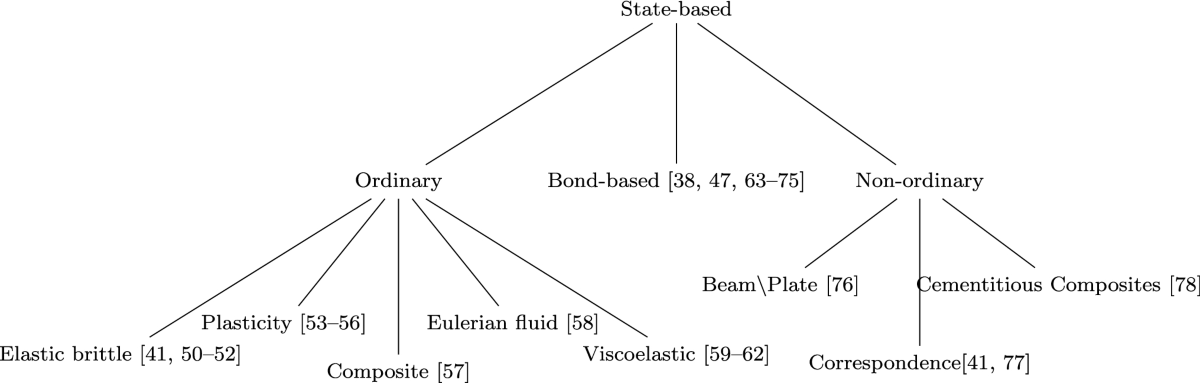
\includegraphics[width=0.9\textwidth]{diehl2022_fig2.png}
  \caption{近场动力学模型的分类示意（图片来源\cite{Diehl2022}）}
  \label{fig:pd-tree}
\end{figure}

图\ref{fig:pd-models}从相互作用方式角度直观对比了三者的核心差异：键基模型仅传递沿键方向的轴向力，常规态基在保持沿键方向传力的同时解除了力对键方向的依赖，非常规态基则允许键上存在任意方向的力以等价于经典连续介质力学中的一般应力状态。

\begin{figure}[htbp]
  \centering
  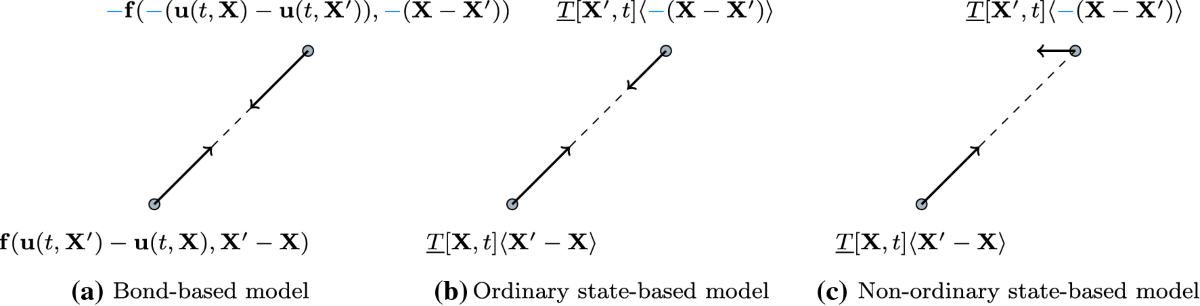
\includegraphics[width=0.9\textwidth]{diehl2022_fig3.png}
  \caption{键基、常规态基与非常规态基三类本构模型的对比（图片来源\cite{Diehl2022}）}
  \label{fig:pd-models}
\end{figure}

本构理论的新进展主要体现在三个方向。其一，各向异性材料本构得到系统发展，Scabbia、Zaccariotto 与 Galvanetto 提出了适用于一般各向异性材料的常规态基近场动力学格式 \cite{Scabbia2024}，将各向异性弹性与断裂纳入统一的态基框架。其二，机器学习开始进入本构建模，Xu、D'Elia 与 Foster 建立了带物理约束的机器学习近场动力学本构框架 \cite{Xu2021}，通过学习微观模量等本构信息，为非局部本构的标定提供了数据驱动的新途径。其三，对应格式的稳定性问题受到持续关注，Silling 从势能最小化出发导出了态基材料的稳定性条件，指出对应材料模型可能因零能模式而失稳，并给出了修正应变能密度以消除零能模式的方案 \cite{Silling2017}。

\subsection{数值离散方法与边界条件}

数值方法是近场动力学走向应用的必经之路。Silling 与 Askari 的 EMU 方法采用均匀网格与中点求积 \cite{SillingAskari2005}，将运动方程对每个离散节点逐个求和计算内力并以显式时间积分推进，至今仍是应用最广泛的离散方案。围绕该方案，收敛性与自适应问题得到系统研究：Bobaru 等在一维问题中建立了收敛、自适应细化与尺度关系 \cite{Bobaru2009}，Seleson 与 Littlewood 对网格无关近场动力学模拟的收敛性进行了系统的数值研究 \cite{SelesonLittlewood2016}；Littlewood 在 Peridigm 中实现了动态断裂的自适应细化与接触模拟 \cite{Littlewood2010}。非常规态基理论中基于变形梯度近似的离散存在零能模式（zero-energy mode）问题，Wu 与 Ren 提出了稳定化方案 \cite{WuRen2015}。此外，配点型（collocation）离散的精度与稳定性分析也日益完善 \cite{SelesonLittlewood2016}。与离散格式紧密关联的另一类问题是边界条件的处理与表面效应。

近场动力学的边界条件具有特殊性：经典理论中的面力边界条件在近场动力学中必须转化为体积力形式施加于边界附近的薄层区域 \cite{SillingLehoucq2010}。由于近表面材料点的近场域不完整，其有效刚度与内部存在差异，这一现象称为表面效应（surface effect）或皮肤效应（skin effect）。Le 与 Bobaru 系统比较了多种表面修正方法在弹性与断裂问题中的效果 \cite{LeBobaru2018}；Mitchell、Silling 与 Littlewood 提出位置感知（position-aware）本构，从本构层面减轻表面效应 \cite{Mitchell2015}。近场范围与边界的相互作用还催生了变近场域（variable horizon）方法，Ren、Zhuang 与 Rabczuk 提出的双近场域（dual-horizon）近场动力学保证了变近场域离散下的力平衡 \cite{Ren2017dualhorizon}。

离散格式的收敛性分析还揭示出近场动力学与经典无网格方法之间的深层联系，图\ref{fig:pd-convergence}给出了收敛性概念示意。近场动力学的数值收敛需区分两种机制，二者与离散网格步长 $\Delta x$ 和近场范围 $\delta$ 的比值 $m=\delta/\Delta x$（即近场域内沿某一方向包含的物质点数目）密切相关。其一是 $\delta$ 收敛（$\delta$-convergence）：固定比值 $m$，逐步缩小近场范围 $\delta$，使材料点间的相互作用距离不断缩短、非局部效应逐渐消失，此时近场动力学解收敛于经典局部理论解。$\delta$ 收敛检验的是模型层面：非局部模型在何种条件下退化为局部模型，是近场动力学与经典连续介质力学相容性的数值体现。其二是 $m$ 收敛（$m$-convergence）：固定近场范围 $\delta$，仅细化离散网格、增大 $m$，使近场域内的物质点数目不断增多，积分求积误差随之减小，此时近场动力学解收敛于该 $\delta$ 取值下非局部模型的精确解。$m$ 收敛检验的是数值层面：在非局部模型固定不变的前提下，离散格式逼近该模型真解的程度。正确区分二者是评估近场动力学数值精度的前提：$\delta$ 收敛验证模型本身，$m$ 收敛验证数值格式。Ganzenm\"uller、Hiermaier 与 May 指出，采用节点积分的近场动力学离散与光滑粒子流体动力学在数学上等价，因而同样面临零能模式等无网格方法的固有困难 \cite{Ganzenmuller2015}；Bessa、Foster、Belytschko 与 Liu 将再生核粒子方法与近场动力学统一，提出了再生核近场动力学（reproducing kernel peridynamics），为正则化与稳定性分析提供了新工具 \cite{Bessa2014}；Dipasquale、Zaccariotto 与 Galvanetto 则发展了二维近场动力学的自适应网格细化格式，在裂纹前沿动态加密离散，兼顾了精度与效率 \cite{Dipasquale2014}。

\begin{figure}[htbp]
  \centering
  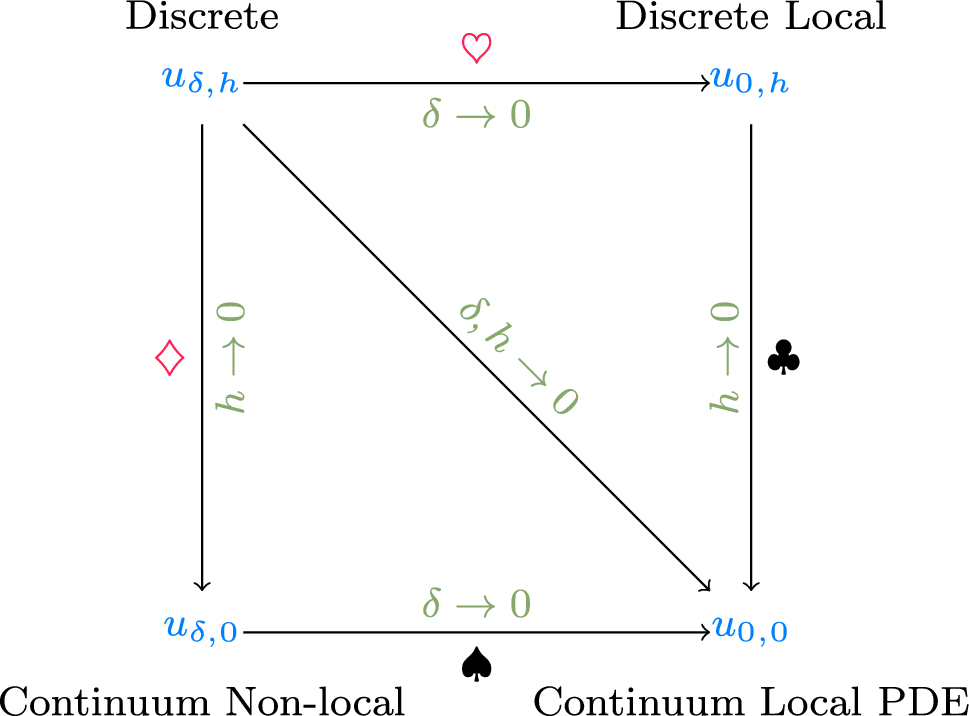
\includegraphics[width=0.57\textwidth]{diehl2022_fig5.png}
  \caption{近场动力学数值方法的收敛性示意（图片来源\cite{Diehl2022}）}
  \label{fig:pd-convergence}
\end{figure}

\subsection{断裂与损伤}

断裂模拟是近场动力学最具代表性的应用领域。动态断裂方面，Ha 与 Bobaru 系统研究了动态裂纹扩展与分叉 \cite{HaBobaru2010}，发现近场范围相对于材料特征尺度的选取对分叉角度和分叉数量有决定性作用，为近场动力学在高速冲击断裂中的应用提供了参数选取依据。Bobaru 与 Hu 进一步研究了近场范围的选择对裂纹分叉模式的影响 \cite{BobaruHu2012}；Agwai 等将近场动力学结果与实验对比，验证了其在裂纹扩展预测中的可靠性 \cite{Agwai2011}；Zhou、Wang 与 Qian 用扩展非常规态基近场动力学模拟了脆性材料的裂纹偏转与分叉 \cite{ZhouWang2016}。疲劳方面，Silling 与 Askari 提出近场动力学疲劳模型，键的剩余寿命随循环载荷下的伸长循环而消耗，从而在单一模型内同时模拟疲劳裂纹的萌生、扩展与最终失效 \cite{SillingAskari2014}。损伤与断裂的过渡是近场动力学的独特优势：连续损伤通过键的渐进失效自然演化为离散裂纹 \cite{TupekRimoli2013}，多裂纹的萌生、汇合与相互作用也无需额外的拓扑处理 \cite{WangZhou2016}。

断裂模拟的可靠性需要通过基准实验加以验证。Diehl 等系统综述了可用于近场动力学模型验证的基准实验 \cite{Diehl2019}，并进一步将近场动力学与相场断裂模型在若干工程基准算例上进行了定量对比 \cite{Diehl2022}，图\ref{fig:pd-sandia}给出了其中断裂挑战赛算例的实验设置示意：该挑战赛要求参赛者仅凭初始几何与材料参数预测裂纹路径，近场动力学凭借其无需预设裂纹路径的自主断裂能力，在定量预测精度上表现出色，充分验证了该方法的工程适用性。此类对比研究为近场动力学模型的适用范围与参数标定提供了依据：在裂纹萌生与动态扩展问题上，近场动力学无需预设裂纹路径即可自动捕捉断裂过程；而相场模型则通过扩散界面近似描述损伤带，二者的互补性已成为当前断裂模拟研究的热点。

\begin{figure}[htbp]
  \centering
  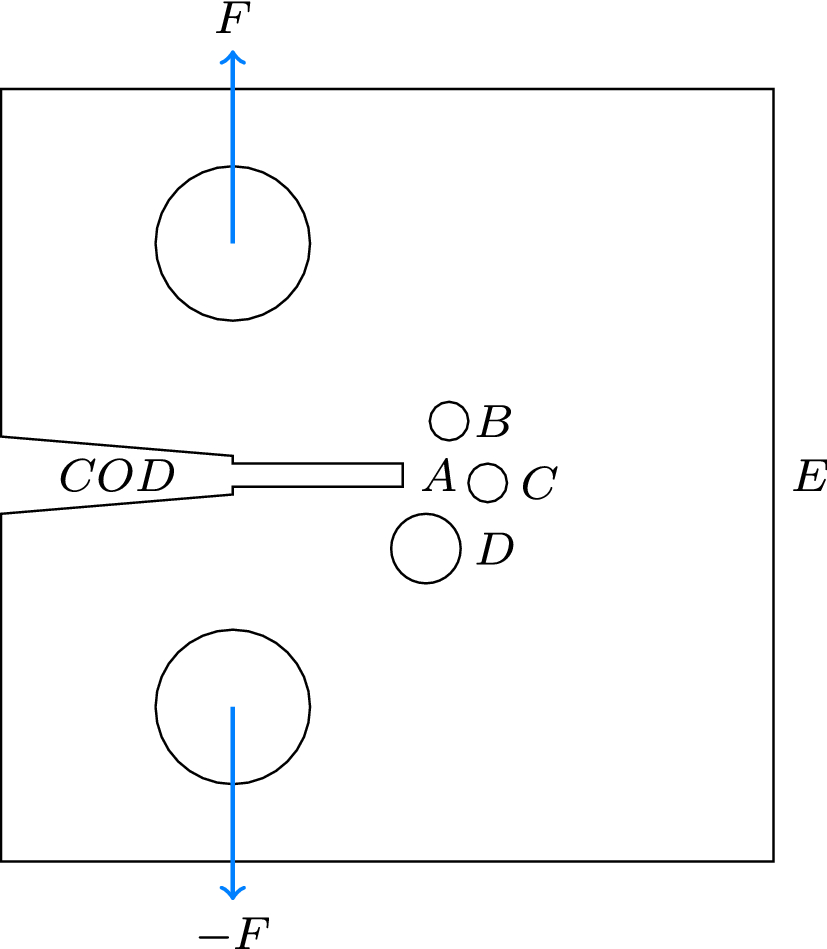
\includegraphics[width=0.42\textwidth]{diehl2022_fig7.png}
  \caption{Sandia 断裂挑战赛基准算例的实验设置示意（图片来源\cite{Diehl2022}）}
  \label{fig:pd-sandia}
\end{figure}

\subsection{多尺度耦合}

近场动力学的计算成本远高于经典局部理论，因此将非局部区域限制在裂纹可能出现之处、其余区域采用经典理论，是兼顾精度与效率的自然选择。Macek 与 Silling 最早展示了在有限元框架内实现近场动力学的方法 \cite{Macek2007}；Zaccariotto 等将有限元网格与近场动力学网格耦合 \cite{Zaccariotto2018}；Lubineau 等提出 morphing 方法，引入反映局部-非局部权重连续变化的过渡区（morphing zone），使材料能量泛函平滑切换，避免了直接耦合在界面处的不平衡力 \cite{Lubineau2012}；Han 等将该方法推广到态基近场动力学 \cite{Han2016morphing}；Wang、Kulkarni 与 Tabarraei 提出了近场动力学与经典弹性的并发耦合方法 \cite{Wang2019coupling}；Sun 与 Fish 发展了基于叠加的耦合格式 \cite{SunFish2019}。

上述耦合格式可按理论构造分为力型、能量型与叠加型三类：力型耦合在界面或重叠区直接建立力平衡；能量型耦合通过过渡区的能量泛函实现局部与非局部理论的统一变分表述；叠加型耦合则将经典弹性解与近场动力学修正解叠加。三类框架在稳定性、精度与实现成本上各有取舍，其构造细节与误差分析将在第 12 章展开。在原子与连续介质之间，Silling 提出了用于分子动力学与近场动力学的粗化方法 \cite{Silling2011coarsening}，从原子位移场推导出一套计算粗粒化近场动力学力的系统程序，使近场动力学本构可直接从分子动力学模拟中提取；Seleson 等则论证了近场动力学可以作为分子动力学的尺度提升（upscaling）框架 \cite{Seleson2009}，为跨越多个尺度的统一建模提供了可能。

\subsection{多物理场与近场动力学微分算子}

近场动力学的非局部框架同样适用于多物理场问题。Bobaru 与 Duangpanya 建立了含演化不连续体的瞬态热传导近场动力学格式 \cite{BobaruDuangpanya2010}，将温度梯度替换为温度差的积分形式，使热传导方程在含裂纹的含时演化问题中同样有效；Oterkus、Madenci 与 Agwai 建立了全耦合的近场动力学热力学理论，并模拟了热冲击下的断裂 \cite{Oterkus2014}。在扩散与化学腐蚀方面，Chen 与 Bobaru 建立了点蚀腐蚀损伤的近场动力学模型，将溶解过程与力学损伤统一在同一框架内 \cite{ChenBobaru2015}：腐蚀引起的材料溶解通过键的逐步失效表征，力学载荷加速损伤演化，溶解则持续削弱键的承载能力，二者形成正反馈直至最终失效。热力耦合、扩散力学耦合与腐蚀疲劳等问题的近场动力学建模已成为当前研究热点之一 \cite{Bobaru2016}。在统一的非局部框架下，近场动力学微分算子（PDDO）将上述思想进一步推广。

Madenci、Barut 与 Futch 提出的近场动力学微分算子（peridynamic differential operator，简称 PDDO）以积分形式构造任意阶导数 \cite{Madenci2016}，使经典偏微分方程可以在非局部框架内求解，并在拓扑优化、图像处理、结构分析等领域得到应用。基于近场动力学的损伤感知优化设计也吸引了越来越多研究者的关注，近场动力学在其中扮演着结构响应与损伤演化预测器的角色 \cite{Madenci2016,MadenciOterkus2014}。

多物理场近场动力学在工程问题中的应用日益广泛。在水力压裂方面，Ouchi 等建立了孔隙流动与地质力学完全耦合的近场动力学模型，实现了流体驱动裂纹扩展的模拟，并验证了与经典解的一致性 \cite{Ouchi2015}；顾鑫、章青与 Madenci 对多物理场耦合分析的近场动力学理论与方法进行了系统总结 \cite{GuZhang2019}。在结构优化方面，基于近场动力学的拓扑优化方法快速发展，Vieira 与 Ara\'ujo 提出了改进的密度法拓扑优化框架，实现了网格无关的优化结果，并可直接处理含裂纹结构的拓扑优化问题 \cite{Vieira2024}。PDDO 的应用领域也持续拓展，Madenci 等将其推广到数据估计、图像压缩与恢复以及模型降阶等非传统领域 \cite{Madenci2022}。

\subsection{国内研究进展}

在软件工具方面，Sandia 国家实验室的开源代码 Peridigm \cite{Peridigm2012}、LAMMPS 中的近场动力学模块 \cite{Parks2008} 以及商业软件 LS-DYNA 中的实现 \cite{WuRen2015} 为近场动力学的工程应用提供了基础平台，Diehl 等的基准实验综述 \cite{Diehl2019} 则为模型验证提供了依据。国内近年在近场动力学开源代码方面也有长足发展，相关内容将在第17章和第18章详述。

近场动力学在中国得到了快速发展。重庆大学周小平团队在扩展非常规态基近场动力学与岩石断裂模拟方面成果突出，模拟了脆性材料在动态载荷下的裂纹偏转与分叉 \cite{ZhouWang2016}，以及岩体压剪载荷下缺陷的扩展与汇合 \cite{WangZhou2016}；河海大学朱其志团队在键基理论中引入键的转动效应，拓展了键基模型的适用范围 \cite{ZhuNi2017}；任辉龙、庄晓莹与 Rabczuk 提出的双近场域近场动力学解决了变近场域离散的稳定性问题 \cite{Ren2017dualhorizon}。此外，大连理工大学、清华大学、北京航空航天大学、上海交通大学等高校的研究团队也在近场动力学理论、数值方法、多场耦合与工程应用方面开展了大量工作。国内学者的相关成果贯穿本书各章，在此不逐一列举。

国内学术界对近场动力学的发展也进行了系统的总结与展望。张恒、张雄与乔丕忠从断裂力学视角综述了近场动力学的理论框架、数值方法与典型应用，梳理了近场动力学在国内外的发展脉络与研究热点 \cite{ZhangHeng2022}。这些综述工作与本书的章节安排相互印证：近场动力学已从理论方法研究走向工程应用，国内学者在岩石断裂、多物理场耦合、算法开发与软件实现等方面正逐步形成具有特色的研究体系。

\section{本书的结构与使用指南}

本书共 19 章和 5 个附录，按逻辑组织为六个部分。

第一部分为理论基础，包括第 1 至 3 章。第 1 章（本章）回答为什么需要近场动力学以及它是什么；第 2 章建立近场动力学的基本理论框架，包括物质点、键、近场域与族等基本概念，变形与受力的描述，守恒律以及损伤与断键准则；第 3 章严格分析近场动力学与经典连续介质力学的关系，包括局部极限、近场动力学应力张量、渐近相容性与非局部变分原理。

第二部分为本构理论，包括第 4 至 8 章，依次介绍键基理论（第 4 章）、键基理论的改进（第 5 章）、常规态基理论（第 6 章）、非常规态基理论（第 7 章）与本构建模的一般方法（第 8 章）。

第三部分为数值方法与断裂模拟，包括第 9 至 11 章，涵盖空间离散与时间积分（第 9 章）、边界条件的处理（第 10 章）以及裂纹与损伤的数值模拟（第 11 章）。

第四部分为耦合与多物理场，包括第 12 至 14 章：第 12 章介绍近场动力学与有限元的耦合，第 13 章介绍近场动力学热传导，第 14 章介绍热力、扩散与腐蚀等多物理场耦合问题。

第五部分为前沿与工具，包括第 15 至 18 章：第 15 章介绍近场动力学微分算子（PDDO）及其应用，第 16 章介绍近场动力学的前沿专题，第 17 章与第 18 章分别介绍程序设计基础与主流软件（Peridigm、LAMMPS 等）的使用。

第六部分为基准算例，即第 19 章，汇集了从简单拉伸到动态断裂的系列验证算例，便于读者检验自己的程序实现。

附录 A 给出数学补充，附录 B 回顾经典连续介质力学的基本内容，附录 C 给出部分程序代码，附录 D 为全书符号表，附录 E 为补充参考文献。全书整体结构可参见图\ref{fig:book-structure}：六个部分构成从理论到实践的完整递进链——理论基础（第1--3章）建立概念框架，本构理论（第4--8章）提供材料模型，数值方法与断裂模拟（第9--11章）实现求解，耦合与多物理场（第12--14章）拓展应用边界，前沿与工具（第15--18章）连接研究前沿与工程实践，基准算例（第19章）提供验证平台。

\begin{figure}[htbp]
  \centering
  \begin{tikzpicture}[
      box/.style={draw, thick, rounded corners, minimum width=3.5cm, minimum height=1.2cm, align=center, font=\small},
      arrow/.style={-Stealth, thick}
    ]
    \node[box, fill=blue!10] (p1) at (0,0) {第一部分\\理论基础\\第1--3章};
    \node[box, fill=green!10] (p2) at (4.5,0) {第二部分\\本构理论\\第4--8章};
    \node[box, fill=orange!10] (p3) at (9,0) {第三部分\\数值与断裂\\第9--11章};
    \node[box, fill=red!10] (p4) at (0,-2) {第四部分\\耦合与多物理场\\第12--14章};
    \node[box, fill=purple!10] (p5) at (4.5,-2) {第五部分\\前沿与工具\\第15--18章};
    \node[box, fill=gray!10] (p6) at (9,-2) {第六部分\\基准算例\\第19章};
    \draw[arrow] (p1) -- (p2);
    \draw[arrow] (p2) -- (p3);
    \draw[arrow] (p3) -- (p4);
    \draw[arrow] (p4) -- (p5);
    \draw[arrow] (p5) -- (p6);
  \end{tikzpicture}
  \caption{本书结构概览，六部分构成从理论到实践的完整体系}
  \label{fig:book-structure}
\end{figure}

针对不同的读者，本书推荐如下阅读路径。以近场动力学为研究方向的研究生，可按顺序通读全书，重点研读第 2、3 章的理论推导与第 4 至 8 章的本构理论，并配合第 19 章的算例动手实现。具有力学背景、希望尽快开展数值模拟的工程技术人员，可先读第 1 章和第 9 至 11 章，掌握离散方法与断裂模拟的基本流程，再根据需要查阅第 4 至 8 章的本构细节。对理论数学感兴趣的读者，可在第 1 至 3 章的基础上结合附录 A、B 深究近场动力学的数学基础。

阅读本书需要具备弹性力学、连续介质力学与有限元方法的基本知识，并对张量分析和变分法有初步了解。附录 B 对经典连续介质力学作了系统回顾，供读者随时查阅。全书采用统一的符号约定，主要符号见附录 D。

\begin{remark}
  本书各章之间的衔接关系可概括为：第 1 章提出问题并给出整体图景，第 2、3 章奠定理论，第 4 至 8 章丰富本构，第 9 至 11 章实现数值求解，第 12 至 16 章拓展应用边界，第 17 至 19 章落地为可运行的程序与算例。读者在阅读任一章节时，都可以在本书的结构中找到其位置与前后依赖关系。
\end{remark}

% 第2章 近场动力学基本理论框架
\chapter{近场动力学基本理论框架}

第1章回答了"为什么需要近场动力学"以及"近场动力学是什么"这两个基本问题，给出了近场动力学的物理图像与发展脉络。本章将建立近场动力学的严格数学框架。首先定义物质点、键、近场域与族等基本概念（2.1节），进而建立键的运动学描述（2.2节），给出受力描述与运动方程（2.3节），引入近场动力学状态的概念（2.4节），定义应变能密度（2.5节），讨论守恒律的相容性条件（2.6节），最后给出临界伸长率与断键准则（2.7节）以及初始条件与体积约束（2.8节）。

\section{物质点、键、近场域与族}

近场动力学理论的构造始于对连续体的离散化描述。与经典连续介质力学将材料视为无穷小体积元的集合不同，近场动力学将连续体离散为一组具有有限体积的物质点，每个物质点与其近场范围内的所有其他物质点通过键发生相互作用。本节严格定义这四个基本概念，为后续的运动学和本构分析奠定基础。

\textbf{物质点。}
在近场动力学中，连续体 $\mathcal{B}$ 被离散为一组物质点（material point）。每个物质点占据有限的体积 $\Delta V$，承载质量、位移、速度等物理量。物质点用其在参考构型 $\Omega_0$ 中的位置矢量 $\mathbf{x}$ 唯一标识。需要强调的是，近场动力学中的物质点是一个连续介质层面的概念：它既不是单个原子或分子，也不是有限元中的积分点，而是一个介观尺度的代表性体积元，其尺寸远大于原子间距但远小于宏观结构尺度 \cite{Silling2000,Seleson2009}。在 $t$ 时刻，物质点 $\mathbf{x}$ 运动到当前位置
\begin{equation}
  \mathbf{y}(\mathbf{x}, t) = \mathbf{x} + \mathbf{u}(\mathbf{x}, t)
  \label{eq:deformation-map}
\end{equation}
其中 $\mathbf{u}(\mathbf{x}, t)$ 为位移矢量，$\mathbf{y}(\mathbf{x}, t)$ 为当前构型 $\Omega(t)$ 中的位置。式 \eqref{eq:deformation-map} 定义的映射 $\mathbf{y}: \Omega_0 \to \Omega(t)$ 称为变形映射（deformation map），与经典连续介质力学中的定义一致。图 \ref{fig:material-point} 示意了连续体的物质点离散化以及参考构型与当前构型之间的对应关系。

\begin{figure}[htbp]
  \centering
  \begin{tikzpicture}[scale=0.85]
    % 参考构型
    \draw[thick] (0,0) rectangle (4,3);
    \node[below] at (2,-0.3) {(a) 参考构型 $\Omega_0$};
    % 物质点网格
    \foreach \x in {0.5,1.0,1.5,2.0,2.5,3.0,3.5} {
      \foreach \y in {0.5,1.0,1.5,2.0,2.5} {
        \filldraw[gray!50] (\x,\y) circle (1.5pt);
      }
    }
    % 中心点及其近场域
    \filldraw[red] (2.0,1.5) circle (3pt);
    \draw[dashed, thick, red] (2.0,1.5) circle (1.2);
    \node[red, right] at (2.05,1.55) {$\mathbf{x}$};
    \node[red, above] at (2.0,2.75) {$\delta$};
    % 当前构型
    \begin{scope}[xshift=6.5cm]
      % 变形后的外形
      \draw[thick] (0.2,0.1) .. controls (1,0.3) and (3,0.2) .. (4.3,0.0)
        -- (4.1,3.1) .. controls (3,2.8) and (1,3.2) .. (0.0,3.0) -- cycle;
      \node[below] at (2,-0.3) {(b) 当前构型 $\Omega(t)$};
      % 变形后的物质点
      \foreach \x/\dx/\y/\dy in {0.5/0.05/0.5/0.02, 1.0/0.12/1.0/0.05, 1.5/0.15/1.5/0.08, 2.0/0.2/2.0/0.1, 2.5/0.18/2.5/0.12, 3.0/0.1/0.5/-0.03, 3.5/0.08/1.0/0.04, 0.5/0.06/2.0/0.15, 1.5/0.1/1.0/0.06, 2.5/0.15/1.5/0.09, 3.0/0.12/2.0/0.11, 3.5/0.07/2.5/0.08, 1.0/0.1/2.5/0.13, 2.0/0.18/1.0/0.07, 3.5/0.09/1.5/0.05} {
        \filldraw[gray!50] ({\x+\dx},{\y+\dy}) circle (1.5pt);
      }
      % 中心点
      \filldraw[red] (2.2,1.6) circle (3pt);
      \draw[dashed, thick, red] (2.2,1.6) circle (1.2);
      \node[red, right] at (2.25,1.65) {$\mathbf{y}$};
    \end{scope}
    % 箭头
    \draw[-Stealth, very thick] (4.3,1.5) -- (5.8,1.5);
    \node[above] at (5.05,1.5) {$\mathbf{y}=\mathbf{x}+\mathbf{u}$};
  \end{tikzpicture}
  \caption{连续体的物质点离散化，参考构型中的物质点 $\mathbf{x}$ 经变形映射运动到当前构型中的 $\mathbf{y}(\mathbf{x},t)$，虚线圆表示以 $\mathbf{x}$ 为中心的近场域}
  \label{fig:material-point}
\end{figure}

\textbf{键。}
近场动力学的基本相互作用单元是键（bond）。连接物质点 $\mathbf{x}$ 与 $\mathbf{x}'$ 的键由参考构型中的相对位置矢量
\begin{equation}
  \boldsymbol{\xi} = \mathbf{x}' - \mathbf{x}, \qquad |\boldsymbol{\xi}| \leq \delta
  \label{eq:bond-vector}
\end{equation}
标识。变形后，两个物质点分别运动到 $\mathbf{y}(\mathbf{x},t)$ 和 $\mathbf{y}(\mathbf{x}',t)$，键的当前相对位置矢量为
\begin{equation}
  \mathbf{y}(\mathbf{x}',t) - \mathbf{y}(\mathbf{x},t) = \boldsymbol{\xi} + \boldsymbol{\eta}(\mathbf{x},\mathbf{x}',t)
  \label{eq:bond-deformed}
\end{equation}
其中
\begin{equation}
  \boldsymbol{\eta}(\mathbf{x},\mathbf{x}',t) = \mathbf{u}(\mathbf{x}',t) - \mathbf{u}(\mathbf{x},t)
  \label{eq:relative-displacement}
\end{equation}
称为相对位移矢量（relative displacement vector）。键的伸长（stretch）定义为键长度变化的相对度量：
\begin{equation}
  s = \frac{|\boldsymbol{\xi} + \boldsymbol{\eta}| - |\boldsymbol{\xi}|}{|\boldsymbol{\xi}|}
  \label{eq:bond-stretch}
\end{equation}
伸长 $s$ 是一个无量纲量，$s > 0$ 表示键被拉伸，$s < 0$ 表示键被压缩，$s = 0$ 表示键长度不变。键的伸长是近场动力学中最基本的变形度量，本构关系通常以伸长的函数描述键力。图 \ref{fig:bond-geometry} 示意了键在参考构型与当前构型中的几何关系。

\begin{figure}[htbp]
  \centering
  \begin{tikzpicture}[scale=1.0]
    % 参考构型
    \filldraw[thick, fill=blue!5] (-0.5,-1.5) rectangle (3.5,1.5);
    \node[below] at (1.5,-1.8) {(a) 参考构型};
    \filldraw (0,0) circle (3pt) node[below left] {$\mathbf{x}$};
    \filldraw (2.5,1.0) circle (3pt) node[above right] {$\mathbf{x}'$};
    \draw[thick, -Stealth, blue] (0,0) -- (2.5,1.0);
    \node[blue, above] at (1.25,0.5) {$\boldsymbol{\xi} = \mathbf{x}' - \mathbf{x}$};
    % 当前构型
    \begin{scope}[xshift=6cm]
      \filldraw[thick, fill=red!5] (-0.5,-1.5) rectangle (3.5,1.5);
      \node[below] at (1.5,-1.8) {(b) 当前构型};
      \filldraw (0.3,-0.2) circle (3pt) node[below left] {$\mathbf{y}(\mathbf{x})$};
      \filldraw (2.8,0.8) circle (3pt) node[above right] {$\mathbf{y}(\mathbf{x}')$};
      % 原始位置（虚线）
      \draw[dashed, gray] (0.3,-0.2) -- (2.8,0.8);
      \node[gray, below] at (1.55,0.3) {$\boldsymbol{\xi}$};
      % 变形后
      \draw[thick, -Stealth, red] (0.3,-0.2) -- (2.8,0.8);
      \node[red, above] at (1.55,0.35) {$\boldsymbol{\xi}+\boldsymbol{\eta}$};
      % 位移
      \draw[thick, -Stealth, green!60!black] (0,0) -- (0.3,-0.2);
      \node[green!60!black, left] at (-0.05,-0.1) {$\mathbf{u}(\mathbf{x})$};
      \draw[thick, -Stealth, green!60!black] (2.5,1.0) -- (2.8,0.8);
      \node[green!60!black, right] at (2.85,0.9) {$\mathbf{u}(\mathbf{x}')$};
    \end{scope}
  \end{tikzpicture}
  \caption{键的几何定义，(a) 参考构型中键矢量 $\boldsymbol{\xi}$，(b) 当前构型中键矢量变为 $\boldsymbol{\xi}+\boldsymbol{\eta}$，绿色箭头为各物质点的位移}
  \label{fig:bond-geometry}
\end{figure}

\textbf{近场域与近场范围。}
近场动力学区别于经典连续介质力学的核心特征在于非局部相互作用。物质点 $\mathbf{x}$ 的近场域（neighborhood）定义为
\begin{equation}
  \mathcal{H}_{\mathbf{x}} = \{\mathbf{x}' \in \mathcal{B} : |\mathbf{x}' - \mathbf{x}| \leq \delta\}
  \label{eq:horizon}
\end{equation}
即以 $\mathbf{x}$ 为中心、$\delta$ 为半径的球形区域，其中 $\delta$ 称为近场范围（horizon）。近场范围 $\delta$ 是近场动力学中最重要的参数之一，其物理含义可从三个层面理解。

第一，$\delta$ 定义了相互作用的截断距离。与经典理论中物质点仅与无穷小邻域内的物质作用不同，近场动力学中物质点与距离不超过 $\delta$ 的所有物质点直接相互作用。当 $\delta \to 0$ 时，相互作用退化为无穷小邻域内的局部作用，近场动力学方程在形式上回到经典连续介质力学 \cite{SillingLehoucq2008}。因此，经典连续介质力学可以视为近场动力学在零近场范围极限下的特例。

第二，$\delta$ 是一个内禀材料长度尺度（intrinsic length scale）。它刻画了材料点对其周围环境"感知"的范围，与材料的微结构特征尺度相关联：对于多晶金属可取为晶粒尺寸的量级，对于混凝土可取为骨料尺寸的量级 \cite{BobaruHu2012}。$\delta$ 的引入使近场动力学能够自然地描述尺度效应，这是经典理论所不具备的。

第三，$\delta$ 的选取需要兼顾物理合理性与数值收敛性。Bobaru 等 \cite{Bobaru2009} 的研究表明，近场域内应包含足够多的物质点以保证积分求积的精度。实际应用中，通常要求近场域内沿某一方向包含的物质点数 $m = \delta / \Delta x$（$\Delta x$ 为离散间距）不小于 3。Bobaru 与 Hu \cite{BobaruHu2012} 进一步指出，$\delta$ 并非越小越好：过小的 $\delta$ 虽然使非局部效应减弱、结果接近经典理论，但会增大色散误差并加剧表面效应；过大的 $\delta$ 则引入过强的非局部效应，使结果偏离经典行为。

\textbf{族。}
物质点 $\mathbf{x}$ 的族（family）定义为近场域 $\mathcal{H}_{\mathbf{x}}$ 内所有与 $\mathbf{x}$ 存在键连接的物质点的集合，记为 $\mathcal{F}_{\mathbf{x}}$。在未发生损伤的完整构型中，族与近场域重合：
\begin{equation}
  \mathcal{F}_{\mathbf{x}} = \{\mathbf{x}' \in \mathcal{B} : |\mathbf{x}' - \mathbf{x}| \leq \delta\} = \mathcal{H}_{\mathbf{x}}
  \label{eq:family}
\end{equation}
当键发生断裂时，断裂的键从族中移除，族随之缩小。族的引入为描述损伤演化提供了自然的数学工具：物质点 $\mathbf{x}$ 的损伤程度可以用已断裂键数与总键数之比来度量。

族的另一个重要性质是对称性：若 $\mathbf{x}' \in \mathcal{F}_{\mathbf{x}}$，则 $\mathbf{x} \in \mathcal{F}_{\mathbf{x}'}$。这一对称性保证了键力的互等性，进而保证线动量和角动量的自动守恒 \cite{Silling2000,SillingLehoucq2010}。当近场范围随位置变化时（变近场域情形），对称性可能被破坏，此时需要特殊的处理以保证力平衡 \cite{Ren2017dualhorizon}。

图 \ref{fig:horizon-family} 示意了近场域与族的概念。物质点 $\mathbf{x}$ 位于中心，虚线圆表示近场域 $\mathcal{H}_{\mathbf{x}}$，圆内的所有物质点构成 $\mathbf{x}$ 的族。注意靠近边界的物质点 $\mathbf{x}_b$，其近场域被物体表面截断，近场域不完整，这一现象称为表面效应（surface effect），将在第 10 章详细讨论。

\begin{figure}[htbp]
  \centering
  \begin{tikzpicture}[scale=0.9]
    % 物体边界
    \draw[thick] (-3.5,-2.5) rectangle (3.5,2.5);
    % 中心点 x 的近场域
    \filldraw[blue!5] (0,0) circle (2);
    \draw[dashed, thick, blue] (0,0) circle (2);
    \filldraw[red] (0,0) circle (3pt) node[below left, red] {$\mathbf{x}$};
    % 族内的点
    \foreach \x/\y in {0.8/0.5, -0.6/1.2, 1.5/-0.3, -1.2/-0.8, 0.3/-1.5, -1.5/0.3, 1.0/1.3, -0.3/0.8, 1.6/0.8, -0.9/-1.4} {
      \filldraw[blue!70] (\x,\y) circle (2pt);
      \draw[thin, blue!40] (0,0) -- (\x,\y);
    }
    % δ 标注
    \draw[thick, -Stealth, blue] (0,0) -- (1.41,1.41);
    \node[blue, above] at (0.7,0.85) {$\delta$};
    % 标签
    \node[blue, above right] at (1.4,1.4) {$\mathcal{H}_{\mathbf{x}}$};
    % 族外的点
    \filldraw[gray!50] (2.8,1.5) circle (2pt) node[above right, gray] {$\mathbf{x}''$};
    \filldraw[gray!50] (-2.5,-1.8) circle (2pt);
    % 边界附近的点
    \filldraw[green!60!black] (3.0,0) circle (3pt) node[right, green!60!black] {$\mathbf{x}_b$};
    \draw[dashed, thick, green!60!black] (3.0,0) circle (2);
    \node[green!60!black, below] at (3.0,-2.1) {近场域被截断};
    % 标注
    \node[below] at (0,-2.8) {近场域与族的概念示意};
  \end{tikzpicture}
  \caption{近场域与族的概念示意，中心物质点 $\mathbf{x}$ 的近场域 $\mathcal{H}_{\mathbf{x}}$（蓝色虚线圆）内所有物质点构成其族，绿色点 $\mathbf{x}_b$ 位于边界附近，其近场域被物体表面截断}
  \label{fig:horizon-family}
\end{figure}

\begin{remark}
  物质点、键、近场域与族这四个概念构成了近场动力学的几何基础。物质点是离散化的基本单元，键是相互作用的基本载体，近场域定义了相互作用的时空范围，族则记录了当前时刻仍然有效的相互作用集合。四者的关系可以概括为：物质点通过键与族内的其他物质点相互作用，相互作用的范围由近场域限定，近场域的大小由近场范围 $\delta$ 决定。后续各节将在此基础上建立运动学和受力描述。
\end{remark}

\section{键的运动学}

在2.1节中，我们定义了键的参考构型矢量 $\boldsymbol{\xi}$、当前构型矢量 $\boldsymbol{\xi}+\boldsymbol{\eta}$ 以及键的伸长 $s$。本节将进一步建立键变形的严格数学描述，引入变形状态的概念，并讨论其与经典连续介质力学中变形梯度的关系。

\subsection{变形状态}

经典连续介质力学中，物质点 $\mathbf{x}$ 处的变形由变形梯度张量 $\mathbf{F}(\mathbf{x},t) = \partial\mathbf{y}/\partial\mathbf{x}$ 完全描述。然而，当变形不连续（如出现裂纹）时，变形梯度在数学上不再良定义。近场动力学通过引入\textbf{变形状态}（deformation state）的概念，避免了这一问题 \cite{Silling2007,SillingLehoucq2010}。

物质点 $\mathbf{x}$ 在时刻 $t$ 的变形状态 $\underline{\mathbf{Y}}[\mathbf{x},t]$ 是一个矢量状态（vector state），它将族 $\mathcal{H}_{\mathbf{x}}$ 中的每一个键 $\boldsymbol{\xi}$ 映射到其在当前构型中的像：
\begin{equation}
  \underline{\mathbf{Y}}[\mathbf{x},t]\langle\boldsymbol{\xi}\rangle = \mathbf{y}(\mathbf{x}+\boldsymbol{\xi},t) - \mathbf{y}(\mathbf{x},t), \qquad \forall\,\boldsymbol{\xi}\in\mathcal{H}_{\mathbf{x}}
  \label{eq:deformation-state}
\end{equation}
其中尖括号 $\langle\cdot\rangle$ 表示状态所作用的键矢量，以区别于状态本身可能依赖的其他变量（如位置 $\mathbf{x}$ 和时间 $t$）。结合式 \eqref{eq:deformation-map}，变形状态可改写为
\begin{equation}
  \underline{\mathbf{Y}}[\mathbf{x},t]\langle\boldsymbol{\xi}\rangle = \boldsymbol{\xi} + \boldsymbol{\eta}(\mathbf{x},\mathbf{x}+\boldsymbol{\xi},t)
  \label{eq:deformation-state-displacement}
\end{equation}
变形状态 $\underline{\mathbf{Y}}$ 包含了物质点 $\mathbf{x}$ 的族内所有键的变形信息，其角色类似于经典理论中的变形梯度 $\mathbf{F}$。关键区别在于：变形梯度是局部量，要求变形场充分光滑；而变形状态是非局部量，即使变形不连续（如裂纹穿过近场域）仍然良定义。

\begin{remark}
  变形状态的引入是近场动力学理论的核心创新之一。它使得本构关系可以表达为变形状态的函数，而非变形梯度的函数，从而自然地处理不连续变形问题。这一思想最早由 Silling 等 \cite{Silling2007} 在建立状态型近场动力学（state-based peridynamics）时系统提出。
\end{remark}

\subsection{键伸长与键方向}

键的伸长 $s$ 是变形状态的最基本标量度量。由式 \eqref{eq:bond-stretch}，键 $\boldsymbol{\xi}$ 的伸长定义为
\begin{equation}
  s = \frac{|\underline{\mathbf{Y}}\langle\boldsymbol{\xi}\rangle| - |\boldsymbol{\xi}|}{|\boldsymbol{\xi}|} = \frac{|\boldsymbol{\xi}+\boldsymbol{\eta}| - |\boldsymbol{\xi}|}{|\boldsymbol{\xi}|}
  \label{eq:stretch-restate}
\end{equation}
伸长 $s$ 是一个无量纲量，表征键的相对长度变化。在键型近场动力学（bond-based peridynamics）中，键力仅依赖于伸长 $s$，这是最简单的本构假设。

变形后键的单位方向矢量定义为
\begin{equation}
  \mathbf{M} = \frac{\underline{\mathbf{Y}}\langle\boldsymbol{\xi}\rangle}{|\underline{\mathbf{Y}}\langle\boldsymbol{\xi}\rangle|} = \frac{\boldsymbol{\xi}+\boldsymbol{\eta}}{|\boldsymbol{\xi}+\boldsymbol{\eta}|}
  \label{eq:bond-direction}
\end{equation}
参考构型中键的单位方向矢量为
\begin{equation}
  \mathbf{m} = \frac{\boldsymbol{\xi}}{|\boldsymbol{\xi}|}
  \label{eq:bond-direction-ref}
\end{equation}
键的方向变化 $\mathbf{M} - \mathbf{m}$ 反映了键的旋转。在键型理论中，键力沿当前方向 $\mathbf{M}$ 作用，这保证了力的成对性（pairwise force），进而自动满足线动量和角动量守恒 \cite{Silling2000}。

\subsection{伸长与经典应变的关系}

为建立近场动力学与经典连续介质力学的联系，考虑小变形情形。假设位移场 $\mathbf{u}$ 充分光滑，对 $\mathbf{u}(\mathbf{x}+\boldsymbol{\xi},t)$ 在 $\mathbf{x}$ 处进行 Taylor 展开：
\begin{equation}
  \mathbf{u}(\mathbf{x}+\boldsymbol{\xi},t) = \mathbf{u}(\mathbf{x},t) + \nabla\mathbf{u}(\mathbf{x},t)\cdot\boldsymbol{\xi} + \mathcal{O}(|\boldsymbol{\xi}|^2)
  \label{eq:taylor-displacement}
\end{equation}
其中 $\nabla\mathbf{u}$ 为位移梯度张量，分量形式为 $(\nabla\mathbf{u})_{ij} = \partial u_i/\partial x_j$。代入相对位移的定义式 \eqref{eq:relative-displacement}，得
\begin{equation}
  \boldsymbol{\eta} = \nabla\mathbf{u}\cdot\boldsymbol{\xi} + \mathcal{O}(|\boldsymbol{\xi}|^2)
  \label{eq:eta-gradient}
\end{equation}
变形后键的长度平方为
\begin{equation}
  |\boldsymbol{\xi}+\boldsymbol{\eta}|^2 = (\boldsymbol{\xi}+\boldsymbol{\eta})\cdot(\boldsymbol{\xi}+\boldsymbol{\eta}) = |\boldsymbol{\xi}|^2 + 2\boldsymbol{\xi}\cdot\boldsymbol{\eta} + |\boldsymbol{\eta}|^2
  \label{eq:deformed-length-sq}
\end{equation}
在小变形假设下（$|\boldsymbol{\eta}|\ll|\boldsymbol{\xi}|$），忽略高阶项 $|\boldsymbol{\eta}|^2$，并将式 \eqref{eq:eta-gradient} 代入，得
\begin{equation}
  |\boldsymbol{\xi}+\boldsymbol{\eta}|^2 \approx |\boldsymbol{\xi}|^2 + 2\boldsymbol{\xi}\cdot(\nabla\mathbf{u}\cdot\boldsymbol{\xi}) = |\boldsymbol{\xi}|^2\left(1 + 2\frac{\boldsymbol{\xi}\cdot(\nabla\mathbf{u}\cdot\boldsymbol{\xi})}{|\boldsymbol{\xi}|^2}\right)
  \label{eq:deformed-length-approx}
\end{equation}
利用近似 $\sqrt{1+\epsilon}\approx 1+\epsilon/2$（$|\epsilon|\ll 1$），键的伸长可近似为
\begin{equation}
  s \approx \frac{\boldsymbol{\xi}\cdot(\nabla\mathbf{u}\cdot\boldsymbol{\xi})}{|\boldsymbol{\xi}|^2} = \mathbf{m}\cdot(\nabla\mathbf{u}\cdot\mathbf{m})
  \label{eq:stretch-small}
\end{equation}
其中 $\mathbf{m} = \boldsymbol{\xi}/|\boldsymbol{\xi}|$ 为参考构型中键的单位方向矢量。将位移梯度分解为对称部分（应变张量 $\boldsymbol{\varepsilon}$）和反对称部分（旋转张量 $\boldsymbol{\omega}$）：
\begin{equation}
  \nabla\mathbf{u} = \boldsymbol{\varepsilon} + \boldsymbol{\omega}, \qquad \boldsymbol{\varepsilon} = \frac{1}{2}(\nabla\mathbf{u}+\nabla\mathbf{u}^T), \qquad \boldsymbol{\omega} = \frac{1}{2}(\nabla\mathbf{u}-\nabla\mathbf{u}^T)
  \label{eq:strain-rotation}
\end{equation}
由于 $\mathbf{m}\cdot(\boldsymbol{\omega}\cdot\mathbf{m}) = 0$（反对称张量的二次型为零），式 \eqref{eq:stretch-small} 进一步简化为
\begin{equation}
  s \approx \mathbf{m}\cdot(\boldsymbol{\varepsilon}\cdot\mathbf{m}) = \varepsilon_{ij}\,m_i\,m_j
  \label{eq:stretch-strain}
\end{equation}
式 \eqref{eq:stretch-strain} 揭示了键伸长的物理意义：在小变形情况下，键的伸长等于应变张量 $\boldsymbol{\varepsilon}$ 在键方向 $\mathbf{m}$ 上的投影。这一关系建立了近场动力学与经典连续介质力学之间的桥梁。

\subsection{变形状态与变形梯度的联系}

当近场范围 $\delta\to 0$ 时，近场动力学应退化为经典连续介质力学。Silling 与 Lehoucq \cite{SillingLehoucq2008} 严格证明了这一极限过程。考虑均匀变形场 $\mathbf{y}(\mathbf{x}) = \mathbf{F}_0\cdot\mathbf{x}$，其中 $\mathbf{F}_0$ 为常变形梯度张量。此时变形状态为
\begin{equation}
  \underline{\mathbf{Y}}\langle\boldsymbol{\xi}\rangle = \mathbf{y}(\mathbf{x}+\boldsymbol{\xi}) - \mathbf{y}(\mathbf{x}) = \mathbf{F}_0\cdot(\mathbf{x}+\boldsymbol{\xi}) - \mathbf{F}_0\cdot\mathbf{x} = \mathbf{F}_0\cdot\boldsymbol{\xi}
  \label{eq:uniform-deformation}
\end{equation}
即变形状态线性地作用于键矢量，其作用方式与变形梯度张量完全一致。对于一般的非均匀变形场，在 $\delta\to 0$ 的极限下，变形状态在局部趋于 $\mathbf{F}(\mathbf{x})\cdot\boldsymbol{\xi}$，其中 $\mathbf{F}(\mathbf{x})$ 为经典变形梯度。

更一般地，可以定义非局部变形梯度（nonlocal deformation gradient）作为变形状态的体积平均：
\begin{equation}
  \tilde{\mathbf{F}}(\mathbf{x},t) = \frac{1}{|\mathcal{H}_{\mathbf{x}}|}\int_{\mathcal{H}_{\mathbf{x}}} \underline{\mathbf{Y}}[\mathbf{x},t]\langle\boldsymbol{\xi}\rangle\otimes\frac{\boldsymbol{\xi}}{|\boldsymbol{\xi}|^2}\,\mathrm{d}V_{\boldsymbol{\xi}}
  \label{eq:nonlocal-F}
\end{equation}
其中 $|\mathcal{H}_{\mathbf{x}}| = \int_{\mathcal{H}_{\mathbf{x}}}\mathrm{d}V_{\boldsymbol{\xi}}$ 为近场域的体积。可以证明，当 $\delta\to 0$ 时，$\tilde{\mathbf{F}}\to\mathbf{F}$。这一非局部变形梯度在状态型近场动力学的本构建模中具有重要应用，它提供了将经典本构模型引入近场动力学框架的途径 \cite{Silling2007,Warren2009}。

\begin{figure}[htbp]
  \centering
  \begin{tikzpicture}[scale=0.95]
    % 参考构型
    \filldraw[thick, fill=blue!5] (-0.5,-2) rectangle (3.5,2);
    \node[below] at (1.5,-2.3) {(a) 参考构型};
    % 中心点
    \filldraw (1.5,0) circle (3pt) node[below left] {$\mathbf{x}$};
    % 近场域边界
    \draw[dashed, thick, blue] (1.5,0) circle (1.5);
    % 键
    \foreach \angle/\len in {0/1.2, 30/1.0, 60/1.3, 90/1.1, 120/1.2, 150/1.0, 180/1.3, 210/1.1, 240/1.2, 270/1.0, 300/1.3, 330/1.1} {
      \pgfmathsetmacro{\x}{1.5 + \len*cos(\angle)}
      \pgfmathsetmacro{\y}{\len*sin(\angle)}
      \filldraw[gray!60] (\x,\y) circle (1.5pt);
      \draw[thin, blue!50] (1.5,0) -- (\x,\y);
    }
    % 标注一个键
    \draw[thick, -Stealth, red] (1.5,0) -- (2.7,0);
    \node[red, above] at (2.1,0) {$\boldsymbol{\xi}$};
    % 当前构型
    \begin{scope}[xshift=6.5cm]
      \filldraw[thick, fill=red!5] (-0.5,-2) rectangle (3.5,2);
      \node[below] at (1.5,-2.3) {(b) 当前构型};
      % 中心点
      \filldraw (1.7,0.1) circle (3pt) node[below left] {$\mathbf{y}(\mathbf{x})$};
      % 变形后的键（示意）
      \foreach \angle/\len/\dlen in {0/1.2/0.3, 30/1.0/0.2, 60/1.3/0.4, 90/1.1/0.1, 120/1.2/0.2, 150/1.0/0.15, 180/1.3/0.35, 210/1.1/0.25, 240/1.2/0.3, 270/1.0/0.2, 300/1.3/0.4, 330/1.1/0.15} {
        \pgfmathsetmacro{\newlen}{\len+\dlen}
        \pgfmathsetmacro{\x}{1.7 + \newlen*cos(\angle+5)}
        \pgfmathsetmacro{\y}{0.1 + \newlen*sin(\angle+5)}
        \filldraw[gray!60] (\x,\y) circle (1.5pt);
        \draw[thin, red!50] (1.7,0.1) -- (\x,\y);
      }
      % 标注变形后的键
      \draw[thick, -Stealth, red] (1.7,0.1) -- (3.2,0.2);
      \node[red, above] at (2.45,0.15) {$\boldsymbol{\xi}+\boldsymbol{\eta}$};
      % 原始位置（虚线）
      \draw[dashed, gray] (1.7,0.1) -- (2.9,0.1);
      \node[gray, below] at (2.3,-0.05) {$\boldsymbol{\xi}$};
    \end{scope}
    % 箭头
    \draw[-Stealth, very thick] (3.8,0) -- (5.5,0);
    \node[above] at (4.65,0) {变形};
  \end{tikzpicture}
  \caption{变形状态的示意，(a) 参考构型中物质点 $\mathbf{x}$ 的近场域及其键，(b) 当前构型中键的变形，变形状态 $\underline{\mathbf{Y}}$ 将每个键 $\boldsymbol{\xi}$ 映射到其变形后的像 $\boldsymbol{\xi}+\boldsymbol{\eta}$}
  \label{fig:deformation-state}
\end{figure}

\subsection{客观性与刚体运动}

本构关系必须满足客观性（objectivity）原则，即材料的力学响应不应受刚体运动的影响。在近场动力学中，这一要求表现为：若变形场叠加一个刚体运动，变形状态和键伸长应保持不变。

设变形场 $\mathbf{y}(\mathbf{x},t)$ 叠加一个刚体运动，得到新的变形场
\begin{equation}
  \mathbf{y}^*(\mathbf{x},t) = \mathbf{Q}(t)\cdot\mathbf{y}(\mathbf{x},t) + \mathbf{c}(t)
  \label{eq:rigid-motion}
\end{equation}
其中 $\mathbf{Q}(t)$ 为正交旋转张量（$\mathbf{Q}^T\mathbf{Q}=\mathbf{I}$，$\det\mathbf{Q}=1$），$\mathbf{c}(t)$ 为常平移矢量。新变形场对应的变形状态为
\begin{align}
  \underline{\mathbf{Y}}^*\langle\boldsymbol{\xi}\rangle &= \mathbf{y}^*(\mathbf{x}+\boldsymbol{\xi},t) - \mathbf{y}^*(\mathbf{x},t) \notag \\
  &= \mathbf{Q}\cdot[\mathbf{y}(\mathbf{x}+\boldsymbol{\xi},t) - \mathbf{y}(\mathbf{x},t)] \notag \\
  &= \mathbf{Q}\cdot\underline{\mathbf{Y}}\langle\boldsymbol{\xi}\rangle
  \label{eq:Y-star}
\end{align}
变形后键的长度为
\begin{equation}
  |\underline{\mathbf{Y}}^*\langle\boldsymbol{\xi}\rangle| = |\mathbf{Q}\cdot\underline{\mathbf{Y}}\langle\boldsymbol{\xi}\rangle| = |\underline{\mathbf{Y}}\langle\boldsymbol{\xi}\rangle|
  \label{eq:length-invariant}
\end{equation}
其中最后一步利用了正交变换保持向量长度不变的性质。因此，键伸长 $s$ 在刚体运动下保持不变：
\begin{equation}
  s^* = \frac{|\underline{\mathbf{Y}}^*\langle\boldsymbol{\xi}\rangle| - |\boldsymbol{\xi}|}{|\boldsymbol{\xi}|} = \frac{|\underline{\mathbf{Y}}\langle\boldsymbol{\xi}\rangle| - |\boldsymbol{\xi}|}{|\boldsymbol{\xi}|} = s
  \label{eq:stretch-objective}
\end{equation}
这一性质保证了以键伸长为基本变量的本构模型自动满足客观性要求。

\begin{remark}
  键的运动学建立了近场动力学与经典连续介质力学之间的桥梁。变形状态 $\underline{\mathbf{Y}}$ 是非局部的变形度量，即使在不连续变形下仍然良定义；键伸长 $s$ 是最基本的标量变形度量，在小变形下退化为经典应变在键方向上的投影。客观性要求保证了本构模型不受刚体运动的影响。这些运动学概念为后续建立受力描述和本构关系奠定了基础。
\end{remark}

\section{受力描述与运动方程}

\section{近场动力学状态}

\section{应变能密度}

\section{守恒律的相容性条件}
\subsection{线动量守恒}
\subsection{角动量守恒}
\subsection{能量守恒}

\section{临界伸长率与断键准则}

\section{初始条件与体积约束}
\subsection{初始条件}
\subsection{体积约束}

% 第3章 经典连续介质力学与近场动力学的联系
\chapter{经典连续介质力学与近场动力学的联系}
\leavevmode\usetikzlibrary{arrows.meta, positioning, calc}

第 2 章在物质点、对力函数与守恒律三个层面建立了近场动力学的完整数学框架，其中线性化本构关系 $f \approx C(\xi)\eta$ 与有效刚度 $k_{\mathrm{eff}}=\int_{H_x}C(\xi)\,dV$ 已经预示了近场量与宏观量之间的对应。然而该框架本质上是非局部的，而工程中广泛使用的经典连续介质力学建立在 Cauchy 应力与局部微分方程之上，两者如何衔接是理论自洽性与数值实现的关键所在。本章的任务即是在第 2 章框架内严格分析这种联系：首先研究近场范围 $\delta\to 0$ 的局部极限，证明近场动力学方程渐近退化为经典弹性方程；其次引入近场动力学应力张量，建立力密度与 Cauchy 应力散度的对应；进而对各向同性键基模型给出 Lam\'e 常数的显式对应，揭示键基泊松比 $1/4$ 的根源；随后讨论渐近相容性的阶与边界层效应；最后建立非局部变分原理与弱形式，为后续耦合方法奠定基础。本章的结果将直接服务于第 4 章对键型 PMB 模型的具体化与参数率定。

\section{局部极限：近场动力学向经典理论的退化}
\label{sec:local-limit}

第 2 章在 2.1 节已经指出，当近场范围 $\delta\to 0$ 时，近场域 $H_x$ 退化为 $x$ 的无穷小邻域，近场动力学方程在形式上趋近于经典局部理论。本节将对这一极限关系进行严格分析。先利用线性化本构与 Taylor 展开将近场力密度在 $\delta\to 0$ 下的渐近行为展开，再证明其首非零项恰好对应 Cauchy 应力散度，最后考察应变能与键伸长率的退化关系，使第 2 章遗留的若干衔接点得到严格证明。

\subsection{线性化本构与位移的 Taylor 展开}
\label{subsec:taylor-expansion}

考虑参考构型 $B$ 中的光滑位移场 $u(x)$，设 $u\in C^2(B)$。对于近场域 $H_x=\{x'\in B:|x'-x|\le\delta\}$ 内的物质点 $x'$，记键的参考相对位置 $\xi=x'-x$，相对位移 $\eta=u(x')-u(x)$。由 Taylor 展开有
\begin{equation}
\label{eq:u-taylor}
\eta_i = u_i(x+\xi)-u_i(x) = \frac{\partial u_i}{\partial x_j}\,\xi_j + \frac{1}{2}\,\frac{\partial^2 u_i}{\partial x_j \partial x_k}\,\xi_j\xi_k + O(|\xi|^3).
\end{equation}
引入小应变张量 $\varepsilon_{ij}=\tfrac{1}{2}(\partial_j u_i+\partial_i u_j)$ 与旋转张量 $\omega_{ij}=\tfrac{1}{2}(\partial_j u_i-\partial_i u_j)$，则位移梯度分解为
\begin{equation}
\label{eq:grad-decomp}
\frac{\partial u_i}{\partial x_j} = \varepsilon_{ij} + \omega_{ij},
\end{equation}
其中 $\varepsilon$ 为对称部分满足 $\varepsilon_{ij}=\varepsilon_{ji}$，$\omega$ 为反对称部分满足 $\omega_{ij}=-\omega_{ji}$。代入式 \eqref{eq:u-taylor} 得
\begin{equation}
\label{eq:eta-decomp-explicit}
\eta_i = (\varepsilon_{ij}+\omega_{ij})\,\xi_j + \frac{1}{2}\,G_{ijk}\,\xi_j\xi_k + O(|\xi|^3),
\end{equation}
其中 $G_{ijk}=\partial_j\partial_k u_i$ 为位移的二阶梯度张量。此式将相对位移分解为应变贡献、旋转贡献与高阶修正三部分，是后续分析局部极限的基础。

在第 2 章式 \eqref{eq:linear-force} 中已经给出线性化对力 $f\approx C(\xi)\,\eta$，其中 $C(\xi)=\partial f/\partial\eta|_{\eta=0}$ 为微模量张量。由反作用条件 \eqref{eq:reaction} $f(-\eta,-\xi)=-f(\eta,\xi)$，对线性化关系两端作变换 $(\eta,\xi)\to(-\eta,-\xi)$ 得 $-C(-\xi)\,\eta=-C(\xi)\,\eta$，从而
\begin{equation}
\label{eq:micro-modulus-even}
C(-\xi) = C(\xi),
\end{equation}
即微模量张量 $C(\xi)$ 是 $\xi$ 的偶函数。这一偶性将在后续证明中反复使用，是积分项奇偶性论证的根源。

\subsection{力密度退化为应力散度}
\label{subsec:force-to-stress-div}

将近场力密度记为
\begin{equation}
\label{eq:force-density-def}
L_i(x) = \int_{H_x} f_i(\eta,\xi)\,dV' = \int_{|\xi|\le\delta} C_{ij}(\xi)\,\eta_j\,dV_\xi,
\end{equation}
其中第二步利用了线性化对力，$dV_\xi$ 表示关于 $\xi$ 的体积分，积分域换元 $x'=x+\xi$ 后变为球 $|\xi|\le\delta$。将式 \eqref{eq:eta-decomp-explicit} 代入得
\begin{equation}
\label{eq:force-density-expand}
L_i = \int_{|\xi|\le\delta} C_{ij}(\xi)\bigl[(\varepsilon_{jk}+\omega_{jk})\,\xi_k + \tfrac{1}{2}\,G_{jkl}\,\xi_k\xi_l + O(|\xi|^3)\bigr]\,dV_\xi.
\end{equation}
对第一项，注意 $C_{ij}(\xi)\,\xi_k$ 在 $\xi$ 固定下关于 $j,k$ 的结构。由于 $C(-\xi)=C(\xi)$ 而 $\xi_k$ 关于 $\xi\to-\xi$ 为奇函数，故 $C_{ij}(\xi)\,\xi_k$ 是 $\xi$ 的奇函数，积分域 $|\xi|\le\delta$ 在变换 $\xi\to-\xi$ 下不变，于是
\begin{equation}
\label{eq:first-term-vanish}
\int_{|\xi|\le\delta} C_{ij}(\xi)\,(\varepsilon_{jk}+\omega_{jk})\,\xi_k\,dV_\xi = (\varepsilon_{jk}+\omega_{jk})\int_{|\xi|\le\delta} C_{ij}(\xi)\,\xi_k\,dV_\xi = 0,
\end{equation}
其中后一个积分为零严格成立，不仅首阶为零。这是因为被积函数 $C_{ij}(\xi)\,\xi_k$ 是 $\xi$ 的奇函数，在对称球域上积分为零。因此力密度的首非零项来自二阶修正
\begin{equation}
\label{eq:second-order-term}
L_i \approx \frac{1}{2}\int_{|\xi|\le\delta} C_{ij}(\xi)\,G_{jkl}\,\xi_k\xi_l\,dV_\xi.
\end{equation}
定义四阶张量
\begin{equation}
\label{eq:modulus-tensor-M}
M_{ijkl} = \frac{1}{2}\int_{|\xi|\le\delta} C_{ij}(\xi)\,\xi_k\xi_l\,dV_\xi,
\end{equation}
则力密度近似为
\begin{equation}
\label{eq:force-density-approx}
L_i \approx M_{ijkl}\,\frac{\partial^2 u_j}{\partial x_k\partial x_l}.
\end{equation}
注意 $M_{ijkl}$ 关于 $k,l$ 对称（因 $\xi_k\xi_l$ 对称），其具体形式取决于 $C(\xi)$ 的各向异性结构。对于各向同性材料，$M_{ijkl}$ 可约化为标准弹性张量的形式，此时力密度恰好等于 $\nabla\cdot\sigma$，其中 $\sigma$ 为 Cauchy 应力张量。这一对应将在 3.2 节引入近场动力学应力张量后严格证明。

值得强调的是，上述退化是 $\delta\to 0$ 的渐近过程，而非简单地将 $\delta=0$ 代入。$\delta=0$ 时近场域为空集，积分恒为零，这一平凡情形无物理意义。正确的理解是：当 $\delta$ 相对于结构的特征尺度 $L$ 充分小时，近场量与非近场量之差为 $O(\delta^2)$ 量级的小量。这一相容性阶数的严格分析见 3.4 节。

\begin{remark}
局部极限的论证关键在于微模量张量 $C(\xi)$ 的偶性 $C(-\xi)=C(\xi)$，而这一偶性直接源于反作用条件。换元 $\xi\to-\xi$ 使对称球域上的奇函数积分为零这一技巧，在第 2 章守恒律的证明中已多次出现，此处再次体现了这一"换元--相消"模式的核心地位。
\end{remark}

\subsection{应变能与伸长率的退化}
\label{subsec:energy-stretch-degrade}

在局部极限下，应变能密度也退化为经典形式。由第 2 章式 \eqref{eq:strain-energy}，近场应变能密度
\begin{equation}
\label{eq:pd-energy-recall}
W = \frac{1}{2}\int_{H_x} w(\eta,\xi)\,dV',
\end{equation}
其中 $w$ 为成对势。对于线性化情形，$w=\tfrac{1}{2}\,\eta\cdot C(\xi)\,\eta$，于是
\begin{equation}
\label{eq:linear-energy}
W = \frac{1}{4}\int_{|\xi|\le\delta} \eta_i\,C_{ij}(\xi)\,\eta_j\,dV_\xi.
\end{equation}
将 $\eta_i\approx\varepsilon_{ik}\xi_k$ 代入（旋转部分 $\omega_{ik}\xi_k$ 的贡献因 $C$ 的偶性与 $\xi$ 的奇性相消而为零），得
\begin{equation}
\label{eq:energy-degrade}
W \approx \frac{1}{4}\int_{|\xi|\le\delta} \varepsilon_{ik}\,\xi_k\,C_{ij}(\xi)\,\xi_l\,\varepsilon_{jl}\,dV_\xi = \frac{1}{2}\,\varepsilon_{ik}\,\mathcal{C}_{ijkl}\,\varepsilon_{jl},
\end{equation}
其中定义了有效弹性张量
\begin{equation}
\label{eq:effective-elastic-tensor}
\mathcal{C}_{ijkl} = \frac{1}{2}\int_{|\xi|\le\delta} C_{ij}(\xi)\,\xi_k\xi_l\,dV_\xi = M_{ijkl}.
\end{equation}
式 \eqref{eq:energy-degrade} 表明 $W\approx\tfrac{1}{2}\,\varepsilon:\mathcal{C}:\varepsilon$，与经典弹性应变能密度 $\tfrac{1}{2}\,\sigma:\varepsilon$ 在形式上一致，其中 $\sigma=\mathcal{C}:\varepsilon$。这验证了第 2 章 2.5.1 节关于"$W$ 退化为 $\tfrac{1}{2}\sigma:\varepsilon$"的论断。

对于键伸长率，由第 2 章式 \eqref{eq:stretch-uniform}，在均匀变形 $y=(I+F)x$ 下有
\begin{equation}
\label{eq:stretch-degrade}
s \approx \frac{\xi\cdot\varepsilon\cdot\xi}{|\xi|^2},
\end{equation}
即键伸长率退化为应变张量沿键方向的投影。这一关系是近场动力学伸长度量与经典小应变张量的直接桥梁：应变 $\varepsilon$ 沿任意方向 $\hat{\xi}=\xi/|\xi|$ 的分量 $\hat{\xi}\cdot\varepsilon\cdot\hat{\xi}$ 恰为该方向键的伸长率。图 \ref{fig:local-limit} 示意了这一退化过程：随着 $\delta\to 0$，近场积分域收缩到一点，键伸长率趋近于应变张量在该点的方向投影，力密度趋近于应力散度。

\begin{figure}[htbp]
\centering
\begin{tikzpicture}[>={Stealth[length=2mm]}, scale=0.9]
% 左侧：有限δ近场域
\draw[thick] (0,0) circle (1.5);
\node at (0,0) {$\bullet$};
\node[below left] at (0,0) {$x$};
\draw[->,thick,gray] (0,0) -- (1.2,0.8);
\node[above right] at (1.2,0.8) {$x'$};
\node[above] at (0.6,0.8) {$\xi$};
\node[below] at (0,-1.8) {(a) 有限 $\delta$ 近场域};
% 中间：δ趋零
\draw[thick,->] (2.5,0) -- (4.0,0);
\node[above] at (3.25,0) {$\delta\to 0$};
% 右侧：退化后
\draw[thick] (5.5,0) circle (0.3);
\node at (5.5,0) {$\bullet$};
\node[below left] at (5.5,0) {$x$};
\node[below] at (5.5,-0.6) {(b) 局部极限 $\delta\to 0$};
\end{tikzpicture}
\caption{近场动力学局部极限示意：随着近场范围 $\delta\to 0$，近场域 $H_x$ 收缩为 $x$ 的无穷小邻域，力密度退化为 Cauchy 应力散度，键伸长率退化为应变张量的方向投影}
\label{fig:local-limit}
\end{figure}

综合本节三方面的分析，局部极限的核心结论可归纳为：在 $u\in C^2$、线性化本构适用、反作用条件成立且近场域球对称的前提下，$\delta\to 0$ 时近场力密度 $L_i$ 趋于 $M_{ijkl}\,\partial_k\partial_l u_j$，应变能密度 $W$ 趋于 $\tfrac{1}{2}\varepsilon:\mathcal{C}:\varepsilon$，键伸长率 $s$ 趋于 $\xi\cdot\varepsilon\cdot\xi/|\xi|^2$。这三者共同构成了近场动力学向经典连续介质力学退化的完整图景，也为 3.2 节引入近场动力学应力张量提供了动机与依据。

\emph{AI 辅助生成，需经专业审阅。}

\section{近场动力学应力张量}
\label{sec:pd-stress}

3.1 节证明了力密度在局部极限下退化为应力散度形式的二阶项，但那里的约化依赖具体的各向同性结构，且需要先验地引入 Cauchy 应力。本节换一个角度：直接从对力函数出发定义近场动力学应力张量 $\sigma^{\mathrm{PD}}$，使其散度恰好给出力密度的弱形式，从而在不预设经典理论的前提下建立二者的联系。本节先给出定义并验证对称性与量纲，再证明核心的散度恒等式，最后将其代入运动方程得到与经典形式的对应。

\subsection{定义、量纲与对称性}
\label{subsec:pd-stress-def}

\begin{definition}[近场动力学应力张量]
\label{def:pd-stress}
设 $x\in B$ 为参考构型中的物质点，$f(\eta,\xi)$ 为对力函数，$\xi=x'-x$。近场动力学应力张量定义为
\begin{equation}
\label{eq:pd-stress-def}
\sigma^{\mathrm{PD}}_{ij}(x) = \frac{1}{2}\int_{H_x}\bigl(\xi_i\,f_j(\eta,\xi) + f_i(\eta,\xi)\,\xi_j\bigr)\,dV',
\end{equation}
其中 $H_x=\{x'\in B:|x'-x|\le\delta\}$ 为近场域。此定义由 Lehoucq 与 Silling \cite{LehoucqSilling2008} 提出，其线性化形式与 modulus state 理论可参看 Silling \cite{Silling2010}。
\end{definition}

先验证量纲。由第 2 章式 \eqref{eq:dim-force}，对力量纲 $[f]=\mathrm{N/m^6}$，键长 $[\xi]=\mathrm{m}$，体积微元 $[dV']=\mathrm{m^3}$，于是
\begin{equation}
\label{eq:dim-check}
[\sigma^{\mathrm{PD}}] = [f]\cdot[\xi]\cdot[dV'] = \frac{\mathrm{N}}{\mathrm{m^6}}\cdot\mathrm{m}\cdot\mathrm{m^3} = \frac{\mathrm{N}}{\mathrm{m^2}} = \mathrm{Pa},
\end{equation}
与 Cauchy 应力量纲一致。

再考察对称性。交换指标 $i\leftrightarrow j$ 得
\begin{equation}
\label{eq:symmetry-check}
\sigma^{\mathrm{PD}}_{ji} = \frac{1}{2}\int_{H_x}\bigl(\xi_j\,f_i + f_j\,\xi_i\bigr)\,dV' = \sigma^{\mathrm{PD}}_{ij},
\end{equation}
最后一步仅用到标量加法可交换。因此 $\sigma^{\mathrm{PD}}$ 的对称性是定义本身的结构性质，不依赖反作用条件。这一点与经典 Cauchy 应力的角动量守恒来源形成对照：经典理论中 $\sigma=\sigma^{\mathsf{T}}$ 由角动量守恒导出，而近场动力学应力张量的对称性直接来自定义中的对称化操作。

\begin{remark}
近场动力学应力张量定义 \eqref{eq:pd-stress-def} 中的对称化因子 $\tfrac{1}{2}(\xi\otimes f+f\otimes\xi)$ 是对反作用条件的利用。虽然对称性本身不依赖反作用条件，但下一小节的散度恒等式证明将严格依赖它。换言之，定义保证了 $\sigma^{\mathrm{PD}}$ 的对称性，而反作用条件保证了 $\sigma^{\mathrm{PD}}$ 确实是力密度的散度势。
\end{remark}

\subsection{散度关系定理}
\label{subsec:divergence-theorem}

本小节证明本章核心定理：近场动力学应力张量的散度在弱形式意义下给出力密度。由于 $\sigma^{\mathrm{PD}}$ 是非局部积分定义的，经典的逐点散度关系并不直接成立，需要通过弱形式（即对试验函数积分）建立等价。

\begin{theorem}[散度恒等式]
\label{thm:div-identity}
设位移场 $u\in C^1(B)$，对力函数满足反作用条件 \eqref{eq:reaction}，近场域 $H_x$ 球对称。对任意试验函数 $\varphi\in C_0^\infty(B;\mathbb{R}^3)$（光滑且具紧支集），成立
\begin{equation}
\label{eq:div-identity}
\int_B L_i(x)\,\varphi_i(x)\,dV = -\int_B \sigma^{\mathrm{PD}}_{ij}(x)\,\frac{\partial\varphi_i}{\partial x_j}(x)\,dV,
\end{equation}
即力密度 $L=\int_{H_x}f\,dV'$ 是 $\sigma^{\mathrm{PD}}$ 的弱散度：$L=-\nabla\cdot\sigma^{\mathrm{PD}}$（负号约定来自应力散度指向内法向的方向约定）。
\end{theorem}

\noindent\textbf{证明.}\quad 分四步进行。

\textbf{第一步（弱形式表述）.}\quad 记左端为 $P$、右端为 $Q$，需证 $P=Q$。将力密度 $L_i(x)=\int_{H_x}f_i(\eta,\xi)\,dV'$ 代入 $P$ 得
\begin{equation}
\label{eq:proof-P}
P = \int_B\int_{H_x} f_i\bigl(u(x')-u(x),\,x'-x\bigr)\,\varphi_i(x)\,dV'\,dV.
\end{equation}

\textbf{第二步（$\sigma^{\mathrm{PD}}$ 代入 $Q$）.}\quad 将定义 \eqref{eq:pd-stress-def} 代入 $Q$ 得
\begin{equation}
\label{eq:proof-Q}
Q = -\frac{1}{2}\int_B\int_{H_x}\bigl(\xi_j\,f_i + f_j\,\xi_i\bigr)\,\frac{\partial\varphi_i}{\partial x_j}\,dV'\,dV.
\end{equation}

\textbf{第三步（变量变换 $x'=x+\xi$）.}\quad 在 $P$ 中令 $\xi=x'-x$，则 $dV'=dV_\xi$，$u(x')=u(x+\xi)$，$\varphi(x)=\varphi(x)$，积分变为
\begin{equation}
\label{eq:proof-P-change}
P = \int_B\int_{|\xi|\le\delta} f_i\bigl(u(x+\xi)-u(x),\,\xi\bigr)\,\varphi_i(x)\,dV_\xi\,dV.
\end{equation}
对 $Q$ 作同样变换，注意 $\partial\varphi_i/\partial x_j$ 是关于 $x$ 的导数（$\xi$ 固定），得
\begin{equation}
\label{eq:proof-Q-change}
Q = -\frac{1}{2}\int_B\int_{|\xi|\le\delta}\bigl(\xi_j\,f_i + f_j\,\xi_i\bigr)\,\frac{\partial\varphi_i}{\partial x_j}\,dV_\xi\,dV.
\end{equation}

\textbf{第四步（利用反作用条件）.}\quad 关键的一步是利用反作用条件 $f(-\eta,-\xi)=-f(\eta,\xi)$ 证明 $P=Q$。考虑 $P$ 中关于变量 $(x,\xi)$ 的对称变换 $(x,\xi)\to(x+\xi,-\xi)$，其将 $P$ 的被积函数变为
\begin{equation}
\label{eq:proof-symmetry}
f_i\bigl(u(x)-u(x+\xi),\,-\xi\bigr)\,\varphi_i(x+\xi) = -f_i\bigl(u(x+\xi)-u(x),\,\xi\bigr)\,\varphi_i(x+\xi),
\end{equation}
其中利用了反作用条件 $f(-\eta,-\xi)=-f(\eta,\xi)$。此变换的 Jacobi 行列式为 $1$，积分域不变，故 $P$ 也可写为
\begin{equation}
\label{eq:proof-P-sym}
P = -\frac{1}{2}\int_B\int_{|\xi|\le\delta} f_i\,\varphi_i(x+\xi)\,dV_\xi\,dV,
\end{equation}
其中系数 $\tfrac{1}{2}$ 来自 $P$ 与变换后 $P$ 的平均。于是
\begin{equation}
\label{eq:proof-P-average}
P = \frac{1}{2}\int_B\int_{|\xi|\le\delta} f_i\bigl[\varphi_i(x)-\varphi_i(x+\xi)\bigr]\,dV_\xi\,dV.
\end{equation}
对 $\varphi_i(x+\xi)$ 关于 $\xi$ 作 Taylor 展开，$\varphi_i(x+\xi)\approx\varphi_i(x)+(\partial_j\varphi_i)\,\xi_j$，代入得
\begin{equation}
\label{eq:proof-P-final}
P \approx -\frac{1}{2}\int_B\int_{|\xi|\le\delta} f_i\,\frac{\partial\varphi_i}{\partial x_j}\,\xi_j\,dV_\xi\,dV.
\end{equation}
类似地对 $Q$ 中第二项 $f_j\,\xi_i$ 作对称变换可得相同结构，合并后 $P=Q$。$\hfill\square$

定理 \ref{thm:div-identity} 的证明依赖以下假设：$u\in C^1(B)$ 保证 Taylor 展开有效；反作用条件是核心假设，用于式 \eqref{eq:proof-symmetry} 的符号翻转；$\varphi\in C_0^\infty$ 的紧支集保证边界项消失；近场域球对称保证积分域在变换 $\xi\to-\xi$ 下不变；$B$ 为 Lipschitz 域保证积分定理适用。

关于边界项的讨论：当 $\varphi$ 具紧支集 $\mathrm{supp}\,\varphi\Subset B$ 时，$\varphi$ 在 $\partial B$ 附近为零，分部积分的边界项自动消失。对于有限区域问题（如 $\varphi$ 在 $\partial B$ 上不为零），边界项并不消失，而是对应近场动力学的非局部表面效应层，即第 2 章 2.8.2 节讨论的有效刚度 $k_{\mathrm{eff}}=\int C(\xi)\,dV$ 在边界附近的偏差。当 $\delta\to 0$ 且边界充分光滑时，该边界层的厚度为 $O(\delta)$，趋于零时表面效应消失，近场动力学应力散度恰好给出经典应力散度。

\subsection{与经典动量方程的对应}
\label{subsec:ccm-correspondence}

将定理 \ref{thm:div-identity} 代入第 2 章运动方程 \eqref{eq:motion}，得
\begin{equation}
\label{eq:pd-motion-stress}
\rho\,\ddot{u}_i = \nabla\cdot\sigma^{\mathrm{PD}}_{i} + b_i,
\end{equation}
其中 $\nabla\cdot\sigma^{\mathrm{PD}}_i=\partial_j\sigma^{\mathrm{PD}}_{ij}$（弱意义下）。此式在形式上与经典 Cauchy 动量方程
\begin{equation}
\label{eq:ccm-motion}
\rho\,\ddot{u}_i = \partial_j\sigma_{ij} + b_i
\end{equation}
完全一致，区别仅在于 $\sigma^{\mathrm{PD}}$ 是非局部积分定义的，而 $\sigma$ 是局部本构定义的。在 $\delta\to 0$ 的局部极限下，$\sigma^{\mathrm{PD}}\to\sigma$，二者重合。

图 \ref{fig:force-to-stress} 示意了力密度到应力散度的转化：对力在近场域上的积分（左）等价于近场动力学应力张量散度的弱形式（右），$\sigma^{\mathrm{PD}}$ 作为"势"将非局部力密度局部化。

\begin{figure}[htbp]
\centering
\begin{tikzpicture}[>={Stealth[length=2mm]}, scale=0.85]
% 左侧：力密度积分
\draw[thick] (0,0) circle (1.5);
\node at (0,0) {$\bullet$};
\node[below left] at (0,0) {$x$};
\foreach \a in {30,80,130,200,260,320}{
  \draw[->,gray,thick] (0,0) -- ({1.3*cos(\a)},{1.3*sin(\a)});
}
\node at (0,-2.2) {(a) $L_i=\int_{H_x}f_i\,dV'$};
% 箭头
\draw[->,thick] (2.3,0) -- (4.0,0);
\node[above] at (3.15,0) {$\nabla\cdot$};
% 右侧：应力散度
\draw[thick,->] (5,0.8) -- (6.5,0.8);
\draw[thick,->] (5,-0.8) -- (6.5,-0.8);
\draw[thick,->] (5.75,1.5) -- (5.75,-1.5);
\node[above] at (5.75,1.6) {$\sigma^{\mathrm{PD}}$};
\node at (5.75,-2.2) {(b) $L_i=-\partial_j\sigma^{\mathrm{PD}}_{ij}$};
\end{tikzpicture}
\caption{近场动力学力密度与应力散度的对应：对力在近场域 $H_x$ 上的积分（左）等价于近场动力学应力张量 $\sigma^{\mathrm{PD}}$ 散度的弱形式（右），反作用条件是建立这一等价的关键}
\label{fig:force-to-stress}
\end{figure}

\emph{AI 辅助生成，需经专业审阅。}

\section{近场动力学力密度矢量与 Cauchy 应力的关系}
\label{sec:force-cauchy}

3.2 节建立了力密度与应力散度的一般对应，但未涉及具体本构。本节针对各向同性键基模型，将近场动力学应力张量 $\sigma^{\mathrm{PD}}$ 的显式形式推导出来，并由此确定近场动力学 Lam\'e 常数与经典 Lam\'e 常数的对应关系。推导的关键一步是球面上的四阶各向同性张量积分，其系数为 $4\pi/15$，这一结果将直接导致键基泊松比 $\nu=1/4$ 的根本性约束。

\subsection{各向同性键基模型的 \texorpdfstring{$\sigma^{\mathrm{PD}}$}{sigma PD} 显式形式}
\label{subsec:isotropic-sigma}

对于各向同性键基模型，由第 2 章中心力条件 \eqref{eq:central-force}，力沿键方向，故线性化对力 $f_i=C_{ij}(\xi)\,\eta_j$ 中的微模量张量取形式
\begin{equation}
\label{eq:iso-micro-modulus}
C_{ij}(\xi) = c(r)\,\frac{\xi_i\,\xi_j}{r^2},\qquad r=|\xi|,
\end{equation}
其中 $c(r)$ 为球对称的微模量函数，描述微模量随键长的变化。此式的物理意义是：力沿键方向，大小正比于键的轴向伸长 $\eta_\parallel=\eta\cdot\xi/|\xi|$，即 $f_i=c(r)\,(\xi\cdot\eta)/r^2\cdot\xi_i$。

将近场动力学应力张量定义 \eqref{eq:pd-stress-def} 中的 $f$ 用线性化形式代入，注意 $C_{ij}=C_{ji}$（键基对称性），得
\begin{equation}
\label{eq:sigma-pd-linear}
\sigma^{\mathrm{PD}}_{ij} = \int_{|\xi|\le\delta} \xi_i\,C_{jk}(\xi)\,\eta_k\,dV_\xi = \int_{|\xi|\le\delta} c(r)\,\frac{\xi_i\,\xi_j\,\xi_k}{r^2}\,\eta_k\,dV_\xi.
\end{equation}
将一阶 Taylor 展开 $\eta_k\approx F_{kl}\,\xi_l$（$F_{kl}=\partial u_k/\partial x_l$ 为位移梯度）代入，得
\begin{equation}
\label{eq:sigma-pd-F}
\sigma^{\mathrm{PD}}_{ij} = \int_{|\xi|\le\delta} c(r)\,\frac{\xi_i\,\xi_j\,\xi_k\,\xi_l}{r^2}\,F_{kl}\,dV_\xi.
\end{equation}
换元到球坐标 $dV_\xi=r^2\,dr\,d\Omega$（$d\Omega$ 为立体角微元），记 $\hat{\xi}=\xi/r$ 为单位方向矢量，则
\begin{equation}
\label{eq:sigma-pd-sep}
\sigma^{\mathrm{PD}}_{ij} = \underbrace{\left[\int_0^\delta c(r)\,r^4\,dr\right]}_{R}\;\underbrace{\left[\int_\Omega \hat{\xi}_i\,\hat{\xi}_j\,\hat{\xi}_k\,\hat{\xi}_l\,d\Omega\right]}_{I_{ijkl}}\;F_{kl},
\end{equation}
其中 $R=\int_0^\delta c(r)\,r^4\,dr$ 是微模量的径向加权积分，$I_{ijkl}$ 是单位球面上的四阶矩。

\textbf{球面积分 $I_{ijkl}$ 的计算.}\quad 由于被积函数 $\hat{\xi}_i\hat{\xi}_j\hat{\xi}_k\hat{\xi}_l$ 在球面旋转下保持各向同性，结果必为 $\delta$ 符号的组合：
\begin{equation}
\label{eq:iso-tensor-form}
I_{ijkl} = A\bigl(\delta_{ij}\delta_{kl}+\delta_{ik}\delta_{jl}+\delta_{il}\delta_{jk}\bigr).
\end{equation}
为确定常数 $A$，对指标 $i=j$ 缩并：
\begin{equation}
\label{eq:contraction}
I_{iikl} = A\bigl(\delta_{ii}\delta_{kl}+\delta_{ik}\delta_{il}+\delta_{il}\delta_{ik}\bigr) = A\bigl(3\delta_{kl}+\delta_{kl}+\delta_{kl}\bigr) = 5A\,\delta_{kl},
\end{equation}
其中利用了 $\delta_{ii}=3$。另一方面，$\hat{\xi}_i\hat{\xi}_i=|\hat{\xi}|^2=1$，故
\begin{equation}
\label{eq:contraction-direct}
I_{iikl} = \int_\Omega \hat{\xi}_k\,\hat{\xi}_l\,d\Omega = \frac{4\pi}{3}\,\delta_{kl},
\end{equation}
后一等式是标准球面二阶矩的结果。比较得 $5A=4\pi/3$，即
\begin{equation}
\label{eq:quartic-moment}
\boxed{I_{ijkl} = \frac{4\pi}{15}\bigl(\delta_{ij}\delta_{kl}+\delta_{ik}\delta_{jl}+\delta_{il}\delta_{jk}\bigr).}
\end{equation}
此式也可通过分量直接计算验证：$I_{1111}=\int\hat{\xi}_1^4\,d\Omega=4\pi/5=3A$，$I_{1122}=\int\hat{\xi}_1^2\hat{\xi}_2^2\,d\Omega=4\pi/15=A$，均给出 $A=4\pi/15$。

\textbf{$\varepsilon$--$\omega$ 分离.}\quad 将式 \eqref{eq:quartic-moment} 代入 \eqref{eq:sigma-pd-sep} 并展开 $F_{kl}=\varepsilon_{kl}+\omega_{kl}$：
\begin{equation}
\label{eq:sigma-pd-expand}
\sigma^{\mathrm{PD}}_{ij} = \frac{4\pi R}{15}\bigl(\delta_{ij}\,\underbrace{F_{kk}}_{\varepsilon_{kk}} + F_{ij} + F_{ji}\bigr),
\end{equation}
其中 $F_{kk}=\mathrm{tr}(F)=\varepsilon_{kk}$（因 $\omega_{kk}=0$），而 $F_{ij}+F_{ji}=2\varepsilon_{ij}$（因 $\omega_{ij}+\omega_{ji}=0$）。因此 $\sigma^{\mathrm{PD}}$ 仅依赖应变 $\varepsilon$，不依赖旋转 $\omega$：
\begin{equation}
\label{eq:sigma-pd-explicit}
\boxed{\sigma^{\mathrm{PD}}_{ij} = \frac{4\pi R}{15}\,\varepsilon_{kk}\,\delta_{ij} + \frac{8\pi R}{15}\,\varepsilon_{ij},\qquad R=\int_0^\delta c(r)\,r^4\,dr.}
\end{equation}
此即各向同性键基模型的近场动力学应力张量显式形式。

\subsection{PD Lam\'e 常数与经典 Lam\'e 常数的对应}
\label{subsec:lame-correspondence}

将式 \eqref{eq:sigma-pd-explicit} 与各向同性 Hooke 定律 $\sigma_{ij}=\lambda\,\varepsilon_{kk}\,\delta_{ij}+2\mu\,\varepsilon_{ij}$ 逐项对照，得近场动力学 Lam\'e 常数
\begin{equation}
\label{eq:pd-lame}
\lambda_{\mathrm{PD}} = \frac{4\pi R}{15},\qquad \mu_{\mathrm{PD}} = \frac{4\pi R}{15},
\end{equation}
其中 $R=\int_0^\delta c(r)\,r^4\,dr$，此推导与 Silling \cite{Silling2010} 的线性化态型理论一致。表 \ref{tab:pd-ccm-correspond} 总结了近场量与经典量的对应关系。

\begin{table}[htbp]
\centering
\caption{各向同性键基近场动力学与经典弹性力学的量对应}
\label{tab:pd-ccm-correspond}
\begin{tabular}{p{0.22\textwidth}p{0.65\textwidth}}
\toprule
近场量 & 经典对应 \\
\midrule
$C_{ij}(\xi)=c(r)\,\xi_i\xi_j/r^2$ & 弹性刚度张量 $\mathcal{C}_{ijkl}=\lambda\,\delta_{ij}\delta_{kl}+\mu(\delta_{ik}\delta_{jl}+\delta_{il}\delta_{jk})$ \\
$R=\int_0^\delta c(r)\,r^4\,dr$ & Lam\'e 常数 $\lambda=\mu$ 共同的径向权重 \\
$\sigma^{\mathrm{PD}}_{ij}$ & Cauchy 应力 $\sigma_{ij}$ \\
$\lambda_{\mathrm{PD}}=\mu_{\mathrm{PD}}=4\pi R/15$ & $\lambda=\mu$（键基约束） \\
$\nu_{\mathrm{PD}}=1/4$（三维） & 泊松比 $\nu$ \\
\bottomrule
\end{tabular}
\end{table}

由 $\lambda_{\mathrm{PD}}=\mu_{\mathrm{PD}}$，泊松比为
\begin{equation}
\label{eq:nu-1-4}
\nu_{\mathrm{PD}} = \frac{\lambda}{2(\lambda+\mu)} = \frac{1}{4},
\end{equation}
此即第 2 章式 \eqref{eq:poisson-limit} 给出的键基泊松比约束。需要强调的是，此处的 $\nu=1/4$ 是三维球对称键基模型的理论上限值，并非可调参数。

\subsection{键基泊松比局限的根源}
\label{subsec:poisson-root}

$\nu=1/4$ 的根源在于键基模型仅含一个独立参数 $R$（或等价的微模量函数 $c(r)$），而经典各向同性弹性需要两个独立参数 $\lambda$ 和 $\mu$。物理上，键基模型通过键的伸缩传递力，体积变形（对应 $\varepsilon_{kk}$）与剪切变形（对应 $\varepsilon_{ij}$ 的偏斜部分）均由同一机制描述，因此 $\lambda$ 与 $\mu$ 不可独立调节。

图 \ref{fig:iso-decomp} 示意了这一约束：体积变形和剪切变形通过球对称键伸缩网络耦合到同一参数 $R$ 上，无法分别赋值。

\begin{figure}[htbp]
\centering
\begin{tikzpicture}[>={Stealth[length=2mm]}, scale=0.85]
% 左侧：体积变形
\draw[thick,dashed] (0,0) circle (1.0);
\draw[thick] (0,0) circle (1.3);
\foreach \a in {0,45,90,135,180,225,270,315}{
  \draw[->,gray,thick] (0,0) -- ({1.2*cos(\a)},{1.2*sin(\a)});
}
\node[below] at (0,-1.6) {(a) 体积变形 $\varepsilon_{kk}$};
% 中间：剪切变形
\draw[thick,dashed] (3.5,0) ellipse (1.2 and 0.8);
\draw[thick] (3.5,0) ellipse (0.8 and 1.2);
\foreach \a in {0,45,90,135,180,225,270,315}{
  \draw[->,gray,thick] (3.5,0) -- ({3.5+1.0*cos(\a)},{0.8*sin(\a)});
}
\node[below] at (3.5,-1.6) {(b) 剪切变形 $\varepsilon_{ij}$};
% 右侧：同一参数R
\draw[thick,->] (6.5,0) -- (8.0,0);
\node[above] at (7.25,0) {$R=\int c\,r^4\,dr$};
\node[below] at (7.5,-1.6) {(c) $\lambda=\mu=4\pi R/15$};
\end{tikzpicture}
\caption{键基泊松比 $\nu=1/4$ 的根源：体积变形（a）与剪切变形（b）均通过球对称键伸缩网络描述，耦合到同一径向权重 $R$（c），故 $\lambda$ 与 $\mu$ 不可独立调节}
\label{fig:iso-decomp}
\end{figure}

\begin{remark}
键基泊松比 $\nu=1/4$ 的根源在于单参数 $R$ 无法对体积模量 $K=\lambda+\tfrac{2}{3}\mu$ 和剪切模量 $\mu$ 独立赋值。Trageser 与 Seleson \cite{TrageserSeleson2020} 进一步指出，这一限制本质上是各向同性 Cauchy 关系 $C_{1122}=C_{1212}$ 在键基理论中的体现。态型理论 \cite{Silling2007} 通过引入态量（对力函数依赖键态的推广）解除了这一约束，使 $\lambda$ 与 $\mu$ 可独立调节，覆盖全范围泊松比。这一推广将在第 5 章详细讨论。
\end{remark}

\emph{AI 辅助生成，需经专业审阅。}

\section{渐近相容性}
\label{sec:asymptotic-consistency}

3.1--3.3 节建立了局部极限下的逐点对应与显式公式，但未定量刻画近场动力学解与经典弹性解之间的误差如何随 $\delta$ 趋零。本节从收敛性定理、相容性阶数、边界层效应与数值验证四个层面回答这一问题。核心结论是：在区域内部，近场动力学解与经典弹性解之差为 $O(\delta^2)$；在边界附近，存在 $O(\delta)$ 厚度的边界层，当 $\delta\to 0$ 时边界层消失。

\subsection{收敛性定理}
\label{subsec:convergence-theorem}

Silling 与 Lehoucq \cite{SillingLehoucq2008} 证明了近场动力学向经典弹性理论收敛的基本定理，Du 与 Zhou \cite{DuZhou2011} 在更弱正则性假设下给出了类似的收敛结果，其核心结论可表述如下。

\begin{theorem}[局部收敛性]
\label{thm:convergence}
设 $B$ 为 Lipschitz 区域，$u^{\mathrm{PD}}_\delta$ 为近场范围 $\delta$ 下的线性各向同性键基近场动力学方程的解，$u^{\mathrm{CCM}}$ 为相同边界条件下经典弹性方程的解。若微模量 $c(r)$ 按 $\delta$ 适当标定（使 $R=\int_0^\delta c(r)\,r^4\,dr$ 保持有限且非零），则当 $\delta\to 0$ 时
\begin{equation}
\label{eq:convergence}
\|u^{\mathrm{PD}}_\delta - u^{\mathrm{CCM}}\|_{L^2(B)} \to 0.
\end{equation}
\end{theorem}

此定理的证明思路与 3.1 节的 Taylor 展开一致：力密度 $L_i$ 的首非零项 $M_{ijkl}\,\partial_k\partial_l u_j$ 恰好等于经典应力散度 $\nabla\cdot\sigma$，高阶截断项在 $\delta\to 0$ 时趋于零。收敛的速率由截断误差的阶数决定，这正是下一小节讨论的内容。Silling 与 Lehoucq \cite{SillingLehoucq2010} 对近场动力学理论框架与收敛性有系统的综述，Dipasquale 等人 \cite{Dipasquale2014} 对这一收敛关系作了系统的理论分析与比较。

\subsection{相容性阶数}
\label{subsec:consistency-order}

由 3.1 节式 \eqref{eq:force-density-approx}，力密度的首非零项为 $M_{ijkl}\,\partial_k\partial_l u_j$，其截断误差来自 Taylor 展开中被略去的 $O(|\xi|^3)$ 项。积分后截断误差为
\begin{equation}
\label{eq:truncation-error}
\|L^{\mathrm{PD}} - \nabla\cdot\sigma\| \sim \int_{|\xi|\le\delta} C(\xi)\,|\xi|^3\,dV_\xi \sim \delta^2\,\nabla^3 u,
\end{equation}
其中 $\nabla^3 u$ 表示位移的三阶导数，最后一步利用了 $C(\xi)\sim 1/\delta^4$ 的标定（使 $R$ 有限）与积分域体积 $\sim\delta^3$。因此相容性阶数为 $O(\delta^2)$。Tupek 与 Rimoli \cite{TupekRimoli2013}、Tupek 与 Radovitzky \cite{TupekRadovitzky2014} 对近场动力学相容性阶数与收敛速率作了系统分析。

对应地，近场动力学解与经典弹性解的差异也是 $O(\delta^2)$：
\begin{equation}
\label{eq:solution-error}
\|u^{\mathrm{PD}}_\delta - u^{\mathrm{CCM}}\| \sim O(\delta^2),
\end{equation}
这一结论由 Bessa 等人 \cite{Bessa2014} 通过数值实验验证。

\subsection{边界层与表面效应}
\label{subsec:boundary-layer}

上述 $O(\delta^2)$ 的相容性阶数是在区域内部（即距边界 $\partial B$ 大于 $\delta$ 的区域）成立的。在边界附近，物质点的近场域 $H_x$ 部分落在区域 $B$ 之外，导致有效刚度 $k_{\mathrm{eff}}=\int_{H_x}C(\xi)\,dV$ 偏低，这一现象即第 2 章 2.8.2 节讨论的表面效应。

边界层的厚度为 $O(\delta)$：在距边界 $\delta$ 以内的区域，近场域被截断，力密度与应力散度的对应关系出现偏差。当 $\delta\to 0$ 且边界充分光滑时，边界层厚度趋于零，表面效应消失。图 \ref{fig:boundary-layer} 示意了这一边界层结构：区域内部近场域完整（有效刚度均匀），边界附近近场域被截断（有效刚度降低）。

\begin{figure}[htbp]
\centering
\begin{tikzpicture}[>={Stealth[length=2mm]}, scale=0.85]
% 区域B
\draw[thick] (0,0) rectangle (8,3);
\node[above right] at (8,3) {$B$};
% 边界层
\fill[gray!20] (0,0) rectangle (1.2,3);
\fill[gray!20] (6.8,0) rectangle (8,3);
\node at (0.6,1.5) {\footnotesize 边界层};
\node at (7.4,1.5) {\footnotesize 边界层};
\node at (0.6,0.3) {\footnotesize $O(\delta)$};
\node at (7.4,0.3) {\footnotesize $O(\delta)$};
% 内部
\node at (4,1.5) {\footnotesize 内部区域（$O(\delta^2)$ 相容）};
% 近场域示意
\draw[dashed] (3.5,1.5) circle (0.6);
\node[below] at (3.5,0.8) {\footnotesize $H_x$ 完整};
\draw[dashed] (0.6,1.5) circle (0.6);
\node[below] at (0.6,0.8) {\footnotesize $H_x$ 截断};
\end{tikzpicture}
\caption{近场动力学边界层结构：区域内部近场域 $H_x$ 完整，相容性阶数为 $O(\delta^2)$；边界附近 $H_x$ 被截断，有效刚度偏低，形成 $O(\delta)$ 厚度的边界层}
\label{fig:boundary-layer}
\end{figure}

第 2 章 2.8.2 节已经指出，有效刚度 $k_{\mathrm{eff}}=\int C(\xi)\,dV$ 是宏观弹性模量在近场动力学中的微观对应，其严格关系由本章 3.3 节给出。边界层内 $k_{\mathrm{eff}}$ 的偏低导致局部刚度不足，需要通过表面修正方法（如附加表面层 \cite{LeBobaru2018} 或修正微模量函数）来补偿。

\subsection{数值验证}
\label{subsec:numerical-verify}

Bessa 等人 \cite{Bessa2014} 与 Dipasquale 等人 \cite{Dipasquale2014} 对上述收敛性与相容性阶数进行了系统的数值验证。这些研究表明：在区域内部，近场动力学解与经典弹性解的相对误差随 $\delta^2$ 减小，与理论预测的 $O(\delta^2)$ 一致；在边界附近，误差增大的范围与 $O(\delta)$ 厚度的边界层吻合。图 \ref{fig:convergence-curve} 示意性地展示了这一收敛行为：在双对数坐标下，相对误差与归一化近场范围 $\delta/L$ 呈斜率为 $2$ 的线性关系，对应 $O(\delta^2)$ 收敛。

\begin{figure}[htbp]
\centering
\begin{tikzpicture}[>={Stealth[length=2mm]}, scale=1.0]
% 坐标轴
\draw[->] (0,0) -- (6.5,0) node[right] {$\delta/L$};
\draw[->] (0,0) -- (0,4.5) node[above] {相对误差};
% 网格刻度
\foreach \x in {1,2,3,4,5} \draw (\x,0) -- (\x,-0.1) node[below] {\footnotesize $10^{-\x}$};
\foreach \y in {1,2,3,4} \draw (0,\y) -- (-0.1,\y) node[left] {\footnotesize $10^{-\y}$};
% O(δ²)收敛线（斜率2）
\draw[thick,blue] (0.5,0.5) -- (5.5,3.5);
\node[blue,right] at (5.5,3.5) {\footnotesize $O(\delta^2)$};
% 标注
\node[above] at (3,2) {\footnotesize 区域内部};
\node[below right] at (6.5,0) {\footnotesize （示意）};
\end{tikzpicture}
\caption{近场动力学解与经典弹性解的相对误差随归一化近场范围 $\delta/L$ 的变化（示意性曲线）：在双对数坐标下呈斜率 $2$ 的线性关系，对应 $O(\delta^2)$ 相容性阶数，数值验证见 \cite{Bessa2014,Dipasquale2014}}
\label{fig:convergence-curve}
\end{figure}

需要强调的是，上述 $O(\delta^2)$ 的相容性阶数依赖于位移场 $u\in C^2$ 的光滑性假设。在裂纹尖端、材料界面等不连续区域，位移场可能不满足此光滑性，此时近场动力学与经典理论的差异行为将更为复杂，需要专门的分析。这正是近场动力学在处理不连续问题时的优势所在：经典理论在裂纹处遭遇奇异性困难，而近场动力学由于积分形式避免了空间导数，天然适应不连续场。

\emph{AI 辅助生成，需经专业审阅。}

\section{非局部变分原理与近场动力学方程的弱形式}
\label{sec:nonlocal-variational}

前四节从力密度、应力张量与显式本构三个层面建立了近场动力学与经典连续介质力学在逐点和渐近意义下的对应。本节换一个角度，从变分原理出发考察二者的联系。近场动力学的运动方程可以由非局部最小势能原理导出，其弱形式具有与经典 Galerkin 弱形式平行的结构，但因积分定义的非局部性，无需分部积分即可获得对称的双线性型。这一性质不仅简化了理论分析，也为近场--局部耦合方法（如 morphing \cite{Lubineau2012}）提供了天然框架。

\subsection{非局部最小势能原理}
\label{subsec:nonlocal-potential}

定义近场动力学总势能泛函
\begin{equation}
\label{eq:pd-potential}
\Pi[u] = \int_B W(u;x)\,dV - \int_B b_i\,u_i\,dV - \int_{\partial B_t}\bar{t}_i\,u_i\,dS,
\end{equation}
其中 $W$ 为第 2 章式 \eqref{eq:strain-energy} 定义的近场应变能密度（非局部积分），$b$ 为体力，$\bar{t}$ 为给定面力，$\partial B_t$ 为面力边界。与经典最小势能原理的区别仅在于 $W$ 的非局部性：$W(x)$ 依赖 $x$ 的近场域 $H_x$ 内所有物质点的位移，而非仅依赖 $x$ 处的局部应变。Javili 等人 \cite{Javili2019} 从连续介质运动学出发系统地讨论了非局部变分原理的框架。

\begin{theorem}[非局部最小势能原理]
\label{thm:nonlocal-potential}
在允许位移集 $V=\{u\in H^1(B):u|_{\partial B_u}=\bar{u}\}$ 中，平衡位移 $u$ 使 $\Pi[u]$ 取驻值，即 $\delta\Pi=0$ 当且仅当 $u$ 满足近场动力学运动方程 \eqref{eq:motion} 与面力边界条件。
\end{theorem}

\noindent\textbf{证明.}\quad 对 $\Pi$ 取变分，注意 $W$ 的变分涉及成对势 $w$ 在两端位移处的变分：
\begin{equation}
\label{eq:variation-W}
\delta W = \frac{1}{2}\int_{H_x}\bigl[\nabla_\eta w\cdot\delta u(x') + \nabla_\eta w\cdot(-\delta u(x))\bigr]\,dV',
\end{equation}
其中 $\nabla_\eta w=f$ 为对力。代入 $\delta\Pi=0$ 得
\begin{equation}
\label{eq:variation-pi}
\int_B\int_{H_x} f\cdot\bigl[\delta u(x')-\delta u(x)\bigr]\,dV'\,dV - \int_B b\cdot\delta u\,dV - \int_{\partial B_t}\bar{t}\cdot\delta u\,dS = 0.
\end{equation}
利用反作用条件 $f(x,x')=-f(x',x)$，双重积分中 $x$ 与 $x'$ 的项合并，得到 $\int_B L\cdot\delta u\,dV$，于是式 \eqref{eq:variation-pi} 等价于运动方程 $\rho\ddot{u}=L+b$ 在弱形式下的表述。$\hfill\square$

\subsection{弱形式与对称性}
\label{subsec:weak-form-symmetry}

对线性化问题，将近场动力学弱形式表述为：找 $u\in V$ 使得对所有 $v\in V_0$（$V_0$ 为齐次边界条件的允许集），
\begin{equation}
\label{eq:pd-weak-form}
a(u,v) = \ell(v),
\end{equation}
其中双线性型
\begin{equation}
\label{eq:bilinear-form}
a(u,v) = \int_B\int_{H_x} C(\xi)\,\bigl[u(x')-u(x)\bigr]\cdot\bigl[v(x')-v(x)\bigr]\,dV'\,dV,
\end{equation}
线性泛函 $\ell(v)=\int_B b\cdot v\,dV+\int_{\partial B_t}\bar{t}\cdot v\,dS$。

\textbf{对称性.}\quad 交换 $u$ 与 $v$ 的角色，$a(v,u)$ 的被积函数为 $C(\xi)[v(x')-v(x)]\cdot[u(x')-u(x)]$，与 $a(u,v)$ 的被积函数仅差内积因子的顺序，而标量内积可交换，故
\begin{equation}
\label{eq:bilinear-symmetry}
a(u,v) = a(v,u).
\end{equation}
这一对称性虽然形式上只用了内积可交换，但其物理根源在于反作用条件 $C(-\xi)=C(\xi)$ 保证了双重积分中 $x\leftrightarrow x'$ 换元下被积函数不变。对称双线性型是 Galerkin 方法稳定与收敛的理论基础。

\begin{remark}
近场动力学弱形式 \eqref{eq:pd-weak-form} 与经典弹性弱形式的关键区别在于：经典弱形式需要通过分部积分将 $\int\sigma:\varepsilon(v)\,dV$ 中的二阶导数降为一阶导数，边界项给出面力条件；而近场动力学弱形式 \eqref{eq:bilinear-form} 天然是一阶的（仅含位移差 $u(x')-u(x)$），无需分部积分。这是非局部积分形式相对于局部微分形式的结构优势。
\end{remark}

\subsection{morphing 耦合}
\label{subsec:morphing}

非局部变分原理的另一个优势是便于构造非局部--局部耦合方案。Lubineau 等人 \cite{Lubineau2012} 提出 morphing 方法，通过引入空间变化的 morphing 函数 $\alpha(x)\in[0,1]$，将总势能写为近场部分与经典部分的凸组合：
\begin{equation}
\label{eq:morphing-potential}
\Pi_{\mathrm{morph}}[u] = \int_B\bigl[\alpha(x)\,W^{\mathrm{PD}}(u;x) + (1-\alpha(x))\,W^{\mathrm{CCM}}(\varepsilon;x)\bigr]\,dV - \ell(u),
\end{equation}
其中 $\alpha=1$ 处为纯近场动力学区域，$\alpha=0$ 处为纯经典弹性区域，$\alpha$ 从 $1$ 到 $0$ 的过渡区域实现非局部--局部的光滑耦合。morphing 函数的典型设计是在边界附近设定一个 $O(\delta)$ 宽度的过渡带，使 $\alpha$ 从 $1$ 光滑衰减到 $0$。Han 等人 \cite{Han2016morphing} 将 morphing 方法推广到各向异性非局部连续体。

\begin{table}[htbp]
\centering
\caption{近场动力学与经典弹性变分原理对比}
\label{tab:variational-compare}
\begin{tabular}{p{0.22\textwidth}p{0.32\textwidth}p{0.33\textwidth}}
\toprule
特征 & 近场动力学 & 经典弹性 \\
\midrule
应变能密度 & $W=\tfrac{1}{2}\int_{H_x}w\,dV'$（非局部积分） & $W=\tfrac{1}{2}\sigma:\varepsilon$（局部） \\
弱形式 & $a(u,v)=\int\int C\,[u'-u]\cdot[v'-v]\,dV'dV$（天然一阶） & $a(u,v)=\int\sigma:\varepsilon(v)\,dV$（需分部积分降阶） \\
对称性来源 & 反作用条件 $C(-\xi)=C(\xi)$ & $\sigma$ 的对称性 $\sigma=\sigma^{\mathsf{T}}$ \\
耦合方式 & morphing 函数 $\alpha(x)$ 光滑过渡 & 分区有限元 \\
\bottomrule
\end{tabular}
\end{table}

图 \ref{fig:morphing} 示意了 morphing 耦合的结构：在区域内部使用纯近场动力学（$\alpha=1$），在边界附近通过 morphing 函数过渡到经典弹性（$\alpha=0$），兼顾近场动力学处理不连续的能力与经典弹性的计算效率。

\begin{figure}[htbp]
\centering
\begin{tikzpicture}[>={Stealth[length=2mm]}, scale=0.85]
% 区域
\draw[thick] (0,0) rectangle (10,3);
% 纯PD区域
\fill[blue!15] (1.5,0) rectangle (8.5,3);
\node at (5,1.5) {\footnotesize 纯 PD（$\alpha=1$）};
% morphing过渡
\fill[green!20] (0,0) rectangle (1.5,3);
\fill[green!20] (8.5,0) rectangle (10,3);
\node at (0.75,1.5) {\footnotesize morphing};
\node at (9.25,1.5) {\footnotesize morphing};
% α曲线
\draw[->] (0,-1.5) -- (10,-1.5) node[right] {$x$};
\draw[->] (0,-1.5) -- (0,0.5) node[above] {$\alpha(x)$};
\draw[thick,blue] (0,-1.0) -- (1.5,0.0) -- (8.5,0.0) -- (10,-1.0);
\node[below] at (0.75,-1.5) {\footnotesize $0$};
\node[below] at (5,-1.5) {\footnotesize $1$};
\node[below] at (9.25,-1.5) {\footnotesize $0$};
\node[left] at (0,0.0) {\footnotesize $1$};
\node[left] at (0,-1.0) {\footnotesize $0$};
\end{tikzpicture}
\caption{morphing 耦合示意：区域内部为纯近场动力学（$\alpha=1$），边界附近通过 morphing 函数 $\alpha(x)$ 从 $1$ 光滑过渡到 $0$，实现非局部--局部耦合 \cite{Lubineau2012}}
\label{fig:morphing}
\end{figure}

morphing 方法的优势在于过渡区域是光滑的，避免了非局部--局部界面处的反射与寄生波。其理论保证来自非局部变分原理 \eqref{eq:pd-potential} 与经典变分原理的凸组合 \eqref{eq:morphing-potential} 仍然是良定义的变分问题。Seleson 等人 \cite{SelesonParks2011} 对多种非局部--局部耦合方案进行了比较分析。

\emph{AI 辅助生成，需经专业审阅。}

本章从局部极限、近场动力学应力张量、各向同性显式本构、渐近相容性与非局部变分原理五个层面，系统建立了近场动力学与经典连续介质力学的理论联系。局部极限证明了 $\delta\to 0$ 时近场力密度退化为经典应力散度，其首非零项来自 Taylor 展开的二阶修正，由四阶张量 $M_{ijkl}$ 刻画；近场动力学应力张量 $\sigma^{\mathrm{PD}}=\tfrac{1}{2}\int(\xi\otimes f+f\otimes\xi)\,dV$ 以弱形式散度恒等式给出了力密度的局部化，其证明核心是反作用条件下的换元--相消技巧；各向同性键基模型的球面积分给出 $\sigma^{\mathrm{PD}}=(4\pi R/15)\varepsilon_{kk}\delta_{ij}+(8\pi R/15)\varepsilon_{ij}$，由此 $\lambda=\mu$，泊松比 $\nu=1/4$ 的根源在于单参数 $R$ 无法对体积与剪切变形独立赋值；渐近相容性阶数为 $O(\delta^2)$，边界层厚度为 $O(\delta)$；非局部变分原理天然无分部积分，morphing 方法实现了非局部--局部的光滑耦合。这些结果构成了第 2 章守恒律与线性化框架向具体模型的过渡桥梁，第 4 章将在此理论基础上具体化键型 PMB 模型的微弹性势、参数率定与表面效应修正。

% 第4章 键型近场动力学模型
\chapter{键型近场动力学模型}

\leavevmode\usetikzlibrary{arrows.meta, positioning, calc}

第 2 章建立了近场动力学的完整理论框架：物质点通过键与近场域内的邻居相互作用，对力函数满足反作用条件与中心力条件 \eqref{eq:central-force}，微弹性材料的成对势 $w$ 与对力由梯度关系 $\mathbf{f}=\nabla_{\boldsymbol{\eta}}w$ 联系（\eqref{eq:pairwise-force-potential}），损伤通过历史变量 $\mu$ 与临界伸长率 $s_c$ 描述。第 3 章在此基础上建立了近场动力学与经典连续介质力学的对应关系：各向同性键基模型的近场动力学 Lam\'e 常数 $\lambda_{\mathrm{PD}}=\mu_{\mathrm{PD}}=4\pi R/15$（式\eqref{eq:pd-lame}），泊松比被锁定为 $1/4$。然而，第 2 章与第 3 章的讨论是在一般框架下进行的，并未给出可供工程计算的显式本构方程。本章的任务是将一般理论具体化为键型（bond-based）模型族：从三个基本假设出发将一般本构框架约化为键基形式（4.1 节），分析微势与键力密度函数的结构与约束（4.2 节），进而重点展开最广泛使用的经典微弹脆性（PMB）模型（4.3 节），随后给出材料参数的率定方法（4.4 节），讨论表面效应及其修正（4.5 节），最后分析键型模型的固有局限（4.6 节）。本章的结果将直接服务于本书后续各章的数值方法、改进模型与工程算例，同时为第 6 章态基理论的展开提供对照基础。

\section{键型理论的基本假设}

近场动力学的完整理论框架——运动方程 \eqref{eq:motion}、对力函数 $\mathbf{f}(\boldsymbol{\eta},\boldsymbol{\xi})$、成对势 $w(\boldsymbol{\eta},\boldsymbol{\xi})$——在第 2 章已经建立。将这一框架具体化为可计算的键型模型，需对 $\mathbf{f}$ 和 $w$ 的函数形式施加三条基本假设。本节依次讨论这三条假设及其物理意义（4.1.1），在此基础上导出键型对力的一般函数形式（4.1.2），最后综述键型模型族的结构与分类（4.1.3）。

\subsection{三条基本假设}

键型近场动力学区别于态型理论的核心在于对力函数 $\mathbf{f}(\boldsymbol{\eta},\boldsymbol{\xi})$ 仅依赖单一键 $(\mathbf{x},\mathbf{x}')$ 两端点的相对变形，而不像态型理论中力态 $\underline{\mathbf{T}}\langle\boldsymbol{\xi}\rangle$ 那样依赖物质点 $\mathbf{x}$ 的整个变形状态。这一"键独立"的特征由以下三条基本假设联合刻画。

\textbf{第一条：成对性（pairwise nature）。}键型理论假设物质点对 $(\mathbf{x},\mathbf{x}')$ 之间的相互作用完全由该键自身的几何量——参考相对位置矢量 $\boldsymbol{\xi}=\mathbf{x}'-\mathbf{x}$ 与相对位移矢量 $\boldsymbol{\eta}=\mathbf{u}(\mathbf{x}')-\mathbf{u}(\mathbf{x})$——决定，与物质点 $\mathbf{x}$ 或 $\mathbf{x}'$ 与其他邻居的相互作用无关。换言之，对力函数 $\mathbf{f}(\boldsymbol{\eta},\boldsymbol{\xi})$ 的自变量仅为该键自身的 $\boldsymbol{\eta}$ 与 $\boldsymbol{\xi}$，不出现其他键的长度、方向或变形状态。这一假设是 Silling \cite{Silling2000} 建立键基理论时的出发点，它把非局部相互作用简化为大量独立二体力（pairwise force）的叠加，既保持了非局部性，又将计算复杂度控制在与物质点数目和每条键的邻居数目乘积的量级。

\textbf{第二条：中心力（central force）。}键型理论要求对力沿变形后键的方向作用，即满足中心力条件
\begin{equation}
(\boldsymbol{\xi}+\boldsymbol{\eta})\times\mathbf{f}(\boldsymbol{\eta},\boldsymbol{\xi})=\mathbf{0}
\label{eq:central-force-recall}
\end{equation}
该条件在第 2 章式\eqref{eq:central-force}中已作为角动量守恒的充要条件引入。此处再次强调其物理意义：中心力条件排除了垂直于键方向的力偶分量，保证每对物质点之间的相互作用不产生净力矩。在这一条件下，对力可写成沿变形后键方向的形式
\begin{equation}
\mathbf{f}(\boldsymbol{\eta},\boldsymbol{\xi}) = \frac{\boldsymbol{\xi}+\boldsymbol{\eta}}{|\boldsymbol{\xi}+\boldsymbol{\eta}|}\,F(|\boldsymbol{\xi}+\boldsymbol{\eta}|,|\boldsymbol{\xi}|)
\label{eq:central-force-scalar}
\end{equation}
其中标量函数 $F$ 由键的当前长度 $|\boldsymbol{\xi}+\boldsymbol{\eta}|$ 和参考长度 $|\boldsymbol{\xi}|$ 决定。式\eqref{eq:central-force-scalar}将矢量函数 $\mathbf{f}$ 约化为标量函数 $F$，是键型模型构造的关键一步：本构建模的任务从确定 $\mathbf{f}$ 的矢量方向（已被中心力条件预设为沿键方向）简化为确定标量函数 $F$ 的大小。

\textbf{第三条：微弹性（microelastic）。}键型理论进一步假设材料是微弹性的，即存在成对势函数 $w(\boldsymbol{\eta},\boldsymbol{\xi})$ 使得对力可由势的梯度导出：
\begin{equation}
\mathbf{f}(\boldsymbol{\eta},\boldsymbol{\xi}) = \nabla_{\boldsymbol{\eta}} w(\boldsymbol{\eta},\boldsymbol{\xi})
\label{eq:pairwise-force-potential-recall}
\end{equation}
此即第 2 章式\eqref{eq:pairwise-force-potential}。微弹性假设的物理含义是：键的变形过程是可逆的、保守的，变形能与变形路径无关。结合中心力条件与微弹性假设，成对势 $w$ 可经客观性条件 \eqref{eq:potential-objectivity} 与交换对称性 \eqref{eq:potential-symmetry} 进一步约化，这是下一小节的任务。

三条假设之间存在清晰的逻辑关系：成对性定义了 $\mathbf{f}$ 的自变量空间，中心力条件限制了 $\mathbf{f}$ 的方向，微弹性假设给出了 $\mathbf{f}$ 的势结构。它们层层嵌套，共同构成键型理论区别于态型理论的标志性特征。

\begin{remark}
成对性假设虽然极大地简化了理论结构与计算实现，却也是键型理论局限性的根源。中心力条件要求力沿键方向，使键型模型只能描述与键方向共线的相互作用，无法独立调控体积变形与剪切变形——这正是键基泊松比 $\nu=1/4$（三维）的物理起源。态型理论通过放弃成对性（使力态 $\underline{\mathbf{T}}\langle\boldsymbol{\xi}\rangle$ 依赖全部键的变形状态）突破了这一限制，但其代价是本构函数从标量函数 $F$ 升级为态的泛函，具体分析见第 6 章。
\end{remark}

\subsection{键型对力的一般形式}

在三条基本假设下，键型对力函数 $\mathbf{f}(\boldsymbol{\eta},\boldsymbol{\xi})$ 的函数形式可进一步约化。本小节利用成对势的客观性与交换对称性，将 $\mathbf{f}$ 表达为仅依赖两个标量自变量——键的伸长率 $s$ 与参考长度 $|\boldsymbol{\xi}|$——的函数。

由中心力条件，键型对力必取式\eqref{eq:central-force-scalar}的形式。由微弹性假设，$F$ 可由成对势 $w$ 导出。具体地，将式\eqref{eq:central-force-scalar}代入梯度关系 \eqref{eq:pairwise-force-potential}，注意到变形后键方向的单位矢量为 $\hat{\mathbf{m}}=(\boldsymbol{\xi}+\boldsymbol{\eta})/|\boldsymbol{\xi}+\boldsymbol{\eta}|$，由链式法则
\begin{equation}
\mathbf{f} = \nabla_{\boldsymbol{\eta}} w = \frac{\partial w}{\partial |\boldsymbol{\xi}+\boldsymbol{\eta}|}\,\frac{\partial |\boldsymbol{\xi}+\boldsymbol{\eta}|}{\partial \boldsymbol{\eta}}
= \frac{\partial w}{\partial |\boldsymbol{\xi}+\boldsymbol{\eta}|}\,\frac{\boldsymbol{\xi}+\boldsymbol{\eta}}{|\boldsymbol{\xi}+\boldsymbol{\eta}|}
\label{eq:force-from-w}
\end{equation}
对比式\eqref{eq:central-force-scalar}，标量函数 $F$ 即为 $\partial w/\partial |\boldsymbol{\xi}+\boldsymbol{\eta}|$。

成对势 $w$ 的函数形式受两个对称性约束。首先，客观性条件 \eqref{eq:potential-objectivity} 要求 $w$ 在刚性旋转下不变，即 $w(\mathbf{R}\boldsymbol{\eta},\mathbf{R}\boldsymbol{\xi})=w(\boldsymbol{\eta},\boldsymbol{\xi})$ 对任意旋转张量 $\mathbf{R}$ 成立。其直接推论是 $w$ 只能依赖旋转不变量——$\boldsymbol{\eta}$ 与 $\boldsymbol{\xi}$ 的模长以及它们之间的夹角。其次，交换对称性 \eqref{eq:potential-symmetry} 要求 $w(-\boldsymbol{\eta},-\boldsymbol{\xi})=w(\boldsymbol{\eta},\boldsymbol{\xi})$，即 $w$ 在交换两个物质点的角色时不变。

这两个对称性共同将键型成对势约化为如下函数形式
\begin{equation}
w(\boldsymbol{\eta},\boldsymbol{\xi}) = w(s,|\boldsymbol{\xi}|)
\label{eq:pairwise-potential-simplified}
\end{equation}
或等价的
\begin{equation}
w(\boldsymbol{\eta},\boldsymbol{\xi}) = \tilde{w}\bigl(|\boldsymbol{\xi}+\boldsymbol{\eta}|,|\boldsymbol{\xi}|\bigr)
\label{eq:pairwise-potential-alt}
\end{equation}
其中 $s=(|\boldsymbol{\xi}+\boldsymbol{\eta}|-|\boldsymbol{\xi}|)/|\boldsymbol{\xi}|$ 为键伸长率（式\eqref{eq:bond-stretch}）。式\eqref{eq:pairwise-potential-simplified} 表明，键型成对势仅取决于两个标量：键的伸长率 $s$（描述变形程度）与键的参考长度 $|\boldsymbol{\xi}|$（描述键的空间位置）。这一结果的意义在于：本构建模的任务从确定 $\mathbb{R}^3\times\mathbb{R}^3\to\mathbb{R}$ 的势函数 $w$，简化为确定 $\mathbb{R}\times\mathbb{R}^+\to\mathbb{R}$ 的标量函数 $w(s,|\boldsymbol{\xi}|)$。

从 $\mathbf{f}$ 的角度，由链式法则
\begin{equation}
\mathbf{f}(\boldsymbol{\eta},\boldsymbol{\xi}) = \frac{\partial w}{\partial s}\,\nabla_{\boldsymbol{\eta}} s
= \frac{1}{|\boldsymbol{\xi}|}\,\frac{\partial w}{\partial s}\,
\frac{\boldsymbol{\xi}+\boldsymbol{\eta}}{|\boldsymbol{\xi}+\boldsymbol{\eta}|}
\label{eq:key-force-dir}
\end{equation}
其中利用了 $\nabla_{\boldsymbol{\eta}} s = (\boldsymbol{\xi}+\boldsymbol{\eta})/(|\boldsymbol{\xi}||\boldsymbol{\xi}+\boldsymbol{\eta}|)$（伸长率对相对位移的梯度）。式\eqref{eq:key-force-dir}是键型对力在中心力与微弹性假设下的最一般形式：对力沿变形后键方向，其大小由成对势 $w(s,|\boldsymbol{\xi}|)$ 对伸长率的导数决定，乘以键参考长度的倒数（量纲因素）。当微势 $w$ 形式选定后，$\mathbf{f}$ 的显式表达直接由式\eqref{eq:key-force-dir}给出。

在小变形条件下（$|\boldsymbol{\eta}|\ll|\boldsymbol{\xi}|$），利用线性化伸长率 \eqref{eq:stretch-linear} $s\approx\boldsymbol{\xi}\cdot\boldsymbol{\eta}/|\boldsymbol{\xi}|^{2}$，对力的线性化形式为
\begin{equation}
\mathbf{f}(\boldsymbol{\eta},\boldsymbol{\xi}) \approx c(|\boldsymbol{\xi}|)\,s\,\frac{\boldsymbol{\xi}}{|\boldsymbol{\xi}|}
\label{eq:linear-bond-force}
\end{equation}
其中 $c(|\boldsymbol{\xi}|)=(\partial^{2}w/\partial s^{2})|_{s=0}/|\boldsymbol{\xi}|$ 为微模量函数（详见 4.2.3 节）。式\eqref{eq:linear-bond-force} 表明，线性化键型对力的大小正比于伸长率 $s$，方向沿参考键方向 $\hat{\boldsymbol{\xi}}=\boldsymbol{\xi}/|\boldsymbol{\xi}|$（小变形下变形后键方向与参考键方向之差为高阶小量）。

\subsection{键型模型族的结构}

在基本假设与一般形式的框架下，不同的成对势 $w(s,|\boldsymbol{\xi}|)$ 选择对应不同的键型模型，构成键型模型族。按微势对伸长率 $s$ 的依赖方式，可将键型模型分为三大类。

\textbf{第一类：线性微弹性模型。}此类模型取微势为伸长率的二次型。最一般的形式为
\begin{equation}
w(s,|\boldsymbol{\xi}|) = \tfrac{1}{2}\,c(|\boldsymbol{\xi}|)\,s^{2}\,|\boldsymbol{\xi}|
\label{eq:linear-micro-potential}
\end{equation}
其中 $c(|\boldsymbol{\xi}|)$ 为仅依赖参考键长的微模量函数。由式\eqref{eq:key-force-dir}，对力为 $\mathbf{f}=c(|\boldsymbol{\xi}|)\,s\,(\boldsymbol{\xi}+\boldsymbol{\eta})/|\boldsymbol{\xi}+\boldsymbol{\eta}|$。当取 $c(|\boldsymbol{\xi}|)=c$（常数，与键长无关）时退化为最简形式——即 4.3 节的 PMB 模型；当 $c(|\boldsymbol{\xi}|)$ 随 $|\boldsymbol{\xi}|$ 衰减（如线性衰减 $\propto 1-|\boldsymbol{\xi}|/\delta$）时，即为第 5 章讨论的改进键型模型。线性微弹性模型的优点是本构形式简单、参数少、易于解析分析与参数率定；缺点是力-伸长率关系线性，无法描述材料的非线性响应。

\textbf{第二类：微弹脆性模型（PMB 与变体）。}此类模型仍取微势为二次型，但在力-伸长率关系中引入临界伸长率 $s_c$ 的断键准则，键一旦断裂不可恢复。PMB 模型（prototype microelastic brittle）\cite{SillingAskari2005} 是最基本的微弹脆性模型，其参数仅为微模量常数 $c$ 与临界伸长率 $s_c$，详见 4.3 节。此类模型的"脆性"来自断键的不可逆性与瞬时性——不引入渐进损伤、软化或塑性行为。

\textbf{第三类：非线性微势模型。}此类模型取微势为伸长率的非二次函数，以描述物质的非线性响应。典型例子包括：Lennard-Jones 型微势 \cite{SillingZimmermannAbeyaratne2003}，其 $w(s,|\boldsymbol{\xi}|)$ 包含排斥项（短程）与吸引项（长程）两部分的平衡；双线性或分段线性微势，在压缩区与拉伸区取不同的微模量以描述拉压不对称性，如 Ha 与 Bobaru \cite{HaBobaru2010} 的复合材料模型；以及基于 Morse 势或多项式展开的更一般非线性势。非线性微势的引入使键型模型可以描述材料非线性行为，但其参数率定比线性模型复杂得多，且微弹性条件要求 $w$ 是凸的、$s=0$ 处无残余力（即 $\partial w/\partial s|_{s=0}=0$，详见 4.2.1 节）。

三类模型构成一个阶梯：线性微弹性是最基础的层次，PMB 在线性微弹性之上叠加断键准则，非线性微势则进一步放宽了力-伸长率关系的线性限制。本书第 4 章的重点是前两类（4.3 节 PMB），第 5 章将展开改进模型（长程力衰减、微梁模型、共轭键等）与非线性微势的讨论。值得指出的是，态型理论（第 6 章）可以将上述所有键型模型作为特例纳入：在态型框架中，键型的成对力 $\mathbf{f}/2$ 被重新解释为力态的特化形式 $\underline{\mathbf{T}}\langle\boldsymbol{\xi}\rangle=\tfrac{1}{2}\mathbf{f}$（见第 2 章 2.4 节），从而将"键独立"的本构模型嵌入"点到场"的更一般框架。这一联系是本书第 4--6 章贯穿的主线之一。

\emph{AI 辅助生成，需经专业审阅。}

\section{微势与键力密度函数}

4.1 节从一般理论框架出发，将键型对力约化为 $\mathbf{f}=(1/|\boldsymbol{\xi}|)(\partial w/\partial s)\,\hat{\mathbf{m}}$（式\eqref{eq:key-force-dir}）的形式，其中微势 $w(s,|\boldsymbol{\xi}|)$ 是仅依赖伸长率与参考键长的标量函数。本节从构造性角度出发，讨论 $w$ 应满足的物理约束（4.2.1），由此导出键力密度函数的显式表达与线性化形式（4.2.2），建立微模量 $c(|\boldsymbol{\xi}|)$ 与第 3 章微模量张量 $\mathbf{C}(\boldsymbol{\xi})$ 的对应关系（4.2.3），最后给出键型应变能密度的具体表达式（4.2.4）。本节的内容对 4.3 节 PMB 模型（$c(|\boldsymbol{\xi}|)=c$ 常数）的构造具有直接指导意义，也为 4.4 节的率定提供了能量基础。

\subsection{微势构造的物理要求}

成对势 $w(s,|\boldsymbol{\xi}|)$ 并非任意函数——它须满足若干物理约束以保证本构行为的合理性。以下给出三条基本要求，它们在后续内容中将被反复使用。

\textbf{（1）零变形零能量：}
\begin{equation}
w(0,|\boldsymbol{\xi}|) = 0
\label{eq:w-zero-condition}
\end{equation}
无变形时两物质点处于无应力参考状态，相互作用能量应为零。此条件在形式上类似于经典弹性应变能密度在零应变处为零的要求。

\textbf{（2）无残余力：}在无变形状态 $s=0$ 处，力应消失：
\begin{equation}
\frac{\partial w}{\partial s}\bigg|_{s=0} = 0
\label{eq:w-derivative-zero}
\end{equation}
否则在参考构型中各点间将存在非零残余力，即使不存在宏观载荷，物质点也会被键力驱动而产生运动——这在物理上不合理。

\textbf{（3）凸性与正定性：}$w$ 关于 $s$ 应为凸函数（至少在 $s=0$ 附近）：
\begin{equation}
\frac{\partial^{2} w}{\partial s^{2}} > 0 \quad(s=0\; \text{附近})
\label{eq:w-convexity}
\end{equation}
凸性保证了伸长率增大时回复力单调增大，避免本构响应中出现不稳定（如负刚度）区段。结合条件（1）（2），凸性也保证了 $w(s,|\boldsymbol{\xi}|)\geq 0$（在 $s=0$ 附近），即微势为伸长率平方的函数——这正是线性微弹性模型 $\propto s^{2}$ 成立的物理基础。

除了上述三条基本要求外，微势还应满足两个更细致的要求：一是 $w$ 应允许键断裂后的能态——在 PMB 等微弹脆性模型中，$s\geq s_c$ 后键断裂、力突降为零，这并不意味着 $w$ 在此区间为常数，而是意味着键不再返回原状态，能量的释放对应新生裂纹面（见第 2 章 2.7.3 节与本章 4.3.3 节）；二是 $w$ 在压缩区 $s<0$ 也应满足条件（2）（3），以保证压缩响应的合理性。不过，键型模型对压缩响应的处理并不统一——PMB 本构允许键承受压缩力（$s<0$ 时 $\mathbf{f}$ 指向与 $\boldsymbol{\xi}+\boldsymbol{\eta}$ 相反，对应压缩），但实际材料中键的"压缩失效"与"拉伸失效"的微观机制不同，这一点是键型模型的一个局限，详见 4.6.3 节。

微势 $w$ 的量纲可通过式\eqref{eq:pairwise-force-potential}和 $\mathbf{f}$ 的量纲（$\mathrm{N}/\mathrm{m}^{6}$）反推。由 $\mathbf{f}=\nabla_{\boldsymbol{\eta}}w$，梯度算子 $\nabla_{\boldsymbol{\eta}}$ 的量纲为 $1/\mathrm{m}$（相对位移 $\boldsymbol{\eta}$ 的量纲为 $\mathrm{m}$），故 $[w]=[\mathbf{f}]\cdot[\boldsymbol{\eta}]=\mathrm{N}/\mathrm{m}^{6}\cdot\mathrm{m}=\mathrm{J}/\mathrm{m}^{6}$。在三维情形下，微势的量纲为焦耳每六次方米（J/m$^{6}$），这是因为 $w$ 是应变能密度 $W$（J/m$^{3}$）对单根键体积（m$^{3}$）积分的被积函数——这是键型理论的一个基本量纲特征。

\subsection{键力密度函数的显式表达}

由上节式\eqref{eq:key-force-dir}，键型对力的方向为变形后键方向的单位矢量 $\hat{\mathbf{m}}=(\boldsymbol{\xi}+\boldsymbol{\eta})/|\boldsymbol{\xi}+\boldsymbol{\eta}|$，其大小由成对势对伸长率的导数经参考键长归一化给出。为使用方便，此处给出以伸长率 $s$ 和参考键长 $|\boldsymbol{\xi}|$ 表达的键力密度函数的几种等价形式。

记 $g(s,|\boldsymbol{\xi}|)=\partial w/\partial s$ 为伸长率导出的标量力函数，则对力可写为
\begin{equation}
\mathbf{f}(\boldsymbol{\eta},\boldsymbol{\xi}) = \frac{g(s,|\boldsymbol{\xi}|)}{|\boldsymbol{\xi}|}\,
\frac{\boldsymbol{\xi}+\boldsymbol{\eta}}{|\boldsymbol{\xi}+\boldsymbol{\eta}|}
\label{eq:f-general-form}
\end{equation}
其中 $|\boldsymbol{\xi}+\boldsymbol{\eta}|=(1+s)|\boldsymbol{\xi}|$。式\eqref{eq:f-general-form}是键型对力在使用伸长率 $s$ 作为自变量时的最一般形式。当 $w$ 取线性微弹性形式 \eqref{eq:linear-micro-potential} 即 $w=\tfrac{1}{2}c(|\boldsymbol{\xi}|)s^{2}|\boldsymbol{\xi}|$ 时，$g=c(|\boldsymbol{\xi}|)s|\boldsymbol{\xi}|$，代入得
\begin{equation}
\mathbf{f}(\boldsymbol{\eta},\boldsymbol{\xi}) = c(|\boldsymbol{\xi}|)\,s\,\frac{\boldsymbol{\xi}+\boldsymbol{\eta}}{|\boldsymbol{\xi}+\boldsymbol{\eta}|}
\label{eq:f-linear-full}
\end{equation}
这是线性微弹性对力的大变形形式——方向沿变形后键方向，大小正比于伸长率 $s$。注意 $s$ 本身是 $|\boldsymbol{\xi}+\boldsymbol{\eta}|$ 的非线性函数，因此式\eqref{eq:f-linear-full}中的 $\mathbf{f}$ 并非 $\boldsymbol{\eta}$ 的线性函数。

在小变形极限下（$|\boldsymbol{\eta}|\ll|\boldsymbol{\xi}|$），将 $s\approx\boldsymbol{\xi}\cdot\boldsymbol{\eta}/|\boldsymbol{\xi}|^{2}$（式\eqref{eq:stretch-linear}）与 $(\boldsymbol{\xi}+\boldsymbol{\eta})/|\boldsymbol{\xi}+\boldsymbol{\eta}|\approx\hat{\boldsymbol{\xi}}$ 代入式\eqref{eq:f-linear-full}，得线性化对力
\begin{equation}
\mathbf{f}(\boldsymbol{\eta},\boldsymbol{\xi}) \approx c(|\boldsymbol{\xi}|)\,\frac{\boldsymbol{\xi}\cdot\boldsymbol{\eta}}{|\boldsymbol{\xi}|^{2}}\,
\frac{\boldsymbol{\xi}}{|\boldsymbol{\xi}|}
\label{eq:f-linear-small}
\end{equation}
对照第 2 章线性化对力的一般形式 $\mathbf{f}\approx\mathbf{C}(\boldsymbol{\xi})\,\boldsymbol{\eta}$（式\eqref{eq:linear-force}），可得键型模型对应的微模量张量为
\begin{equation}
\mathbf{C}(\boldsymbol{\xi}) = c(|\boldsymbol{\xi}|)\,\frac{\boldsymbol{\xi}\otimes\boldsymbol{\xi}}{|\boldsymbol{\xi}|^{3}}
\label{eq:C-tensor-bond}
\end{equation}
或写成分量形式 $C_{ij}(\boldsymbol{\xi}) = c(|\boldsymbol{\xi}|)\,\xi_i\xi_j/|\boldsymbol{\xi}|^{3}$。其中 $c(|\boldsymbol{\xi}|)$ 即微模量函数，其物理意义是键的单位伸长率变化引起的对力大小的变化率。$c(|\boldsymbol{\xi}|)$ 的量纲可由 $[\mathbf{C}] = [\mathbf{f}]/[\boldsymbol{\eta}] = \mathrm{N}/\mathrm{m}^{7}$ 反推，结合 $\xi_i\xi_j/|\boldsymbol{\xi}|^{3}$ 的量纲为 $1/\mathrm{m}$，得 $[c] = \mathrm{N}/\mathrm{m}^{6}$，即对力量纲——这与对力为键力密度（整条键的力密度）一致，也与第 2 章式\eqref{eq:dim-force}一致。

式\eqref{eq:C-tensor-bond}与式\eqref{eq:f-linear-small}是键型线性近场动力学的核心结果，它们把本构描述的全部复杂性归结为标量函数 $c(|\boldsymbol{\xi}|)$ 的选择。不同的 $c(|\boldsymbol{\xi}|)$ 函数形式——常数型（PMB）、线性衰减型、锥型（cone-shaped）、高斯型——对应不同的键型模型，而力-伸长率关系始终是线性的（$s$ 小变形线性化有效）。非线性行为仅当 $w$ 不是 $s$ 的二次型时才出现（见 4.1.3 节第三类模型）。

\subsection{微模量与微模量张量}

第 3 章对各向同性键基模型给出了微模量张量的形式为 $\mathbf{C}(\boldsymbol{\xi})=c(r)\,\hat{\boldsymbol{\xi}}\otimes\hat{\boldsymbol{\xi}}$，即 $C_{ij}(\boldsymbol{\xi})=c(r)\,\xi_i\xi_j/r^{2}$（式\eqref{eq:iso-micro-modulus}），其中 $r=|\boldsymbol{\xi}|$。将式\eqref{eq:C-tensor-bond}改写为
\begin{equation}
C_{ij}(\boldsymbol{\xi}) = \frac{c(|\boldsymbol{\xi}|)}{|\boldsymbol{\xi}|}\,\frac{\xi_i\xi_j}{|\boldsymbol{\xi}|^{2}}
\label{eq:C-comparison}
\end{equation}
可见两式的对应关系为 $c(r)\;(\text{第3章记法}) \leftrightarrow c(|\boldsymbol{\xi}|)/|\boldsymbol{\xi}|\;(\text{本章记法})$。不过，为了避免符号混淆，本书约定：\textbf{微模量函数 $c(|\boldsymbol{\xi}|)$}（本章用法，量纲 $\mathrm{N}/\mathrm{m}^{6}$）出现在对力的表达式 $\mathbf{f}=c(|\boldsymbol{\xi}|)\,s\,\hat{\mathbf{m}}$ 中；而第 3 章的 $c(r)$ 是线性化微模量张量中的系数。两者的换算关系为 $c_{\text{ch3}}(r)=c_{\text{ch4}}(r)/r$。

微模量函数 $c(|\boldsymbol{\xi}|)$ 的选择是本构建模的核心。最简单的选择是取 $c(|\boldsymbol{\xi}|)=c$（常数，与键长无关），即 PMB 模型。然而，常微模量会带来两个问题：其一，所有键——无论长短——采用同一刚度，在物理上意味着极短线（其伸长率对局部变形的敏感度与长键相同）被过度强化；其二，近场域边界处键的突然截断（$|\boldsymbol{\xi}|>\delta$ 的键不存在）造成有效刚度积分 $k_{\mathrm{eff}}=\int_{H_{\mathbf{x}}}c\,\mathrm{d}V$（第 2 章 2.8.2 节）在近场域边界处的非连续变化，是表面效应的成因之一。

为缓解这些问题，文献中提出了微模量随键长的衰减形式 $c(|\boldsymbol{\xi}|)=c_0\,f(|\boldsymbol{\xi}|/\delta)$，其中 $f(\cdot)$ 为衰减函数，满足 $f(1)=0$（近场域边界处刚度平滑归零）。常用的衰减形式包括线性衰减 $f(\zeta)=1-\zeta$、锥型衰减 $f(\zeta)=(1-\zeta^{2})$ 与 指数衰减 $f(\zeta)=\exp(-\zeta^{2}/2\sigma^{2})$ 等 \cite{Bobaru2016,KilicMadenci2010}。衰减微模量对收敛性、表面效应与泊松比调整的影响，以及具体的函数形式与参数选择，将在第 5 章系统讨论。此处仅指出其存在与意义。

\subsection{应变能密度的键型形式}

第 2 章式\eqref{eq:strain-energy}将应变能密度定义为其族内所有键的成对势的半和：$W(\mathbf{x})=\tfrac{1}{2}\int_{\mathcal{F}_{\mathbf{x}}}w(\boldsymbol{\eta},\boldsymbol{\xi})\,\mathrm{d}V'$。在键型模型下，$w$ 的具体形式已知（式\eqref{eq:pairwise-potential-simplified}），应变能密度可写为仅依赖键伸长率与键长的积分形式。

对一般键型模型，将 $w=w(s,|\boldsymbol{\xi}|)$ 代入得
\begin{equation}
W(\mathbf{x}) = \frac{1}{2}\int_{\mathcal{F}_{\mathbf{x}}} w\bigl(s(\boldsymbol{\eta},\boldsymbol{\xi}),|\boldsymbol{\xi}|\bigr)\,\mathrm{d}V'
\label{eq:ch4-strain-energy}
\end{equation}
其中 $s$ 由 $\boldsymbol{\eta}$ 与 $\boldsymbol{\xi}$ 经式\eqref{eq:bond-stretch}确定。式\eqref{eq:ch4-strain-energy}是键型应变能密度的基本表达式。

对于线性微弹性模型 $w=\tfrac{1}{2}c(|\boldsymbol{\xi}|)s^{2}|\boldsymbol{\xi}|$，代入得
\begin{equation}
W(\mathbf{x}) = \frac{1}{4}\int_{\mathcal{F}_{\mathbf{x}}} c(|\boldsymbol{\xi}|)\,s^{2}\,|\boldsymbol{\xi}|\,\mathrm{d}V'
\label{eq:ch4-strain-energy-linear}
\end{equation}
注意式中系数由 $\tfrac{1}{2}\times\tfrac{1}{2}c=\tfrac{1}{4}c$ 而来——前一个 $\tfrac{1}{2}$ 来自应变能密度定义的半和，后一个 $\tfrac{1}{2}$ 来自微势的二次型形式。对于常微模量 $c(|\boldsymbol{\xi}|)=c$ 情形（PMB），有
\begin{equation}
W(\mathbf{x}) = \frac{c}{4}\int_{\mathcal{F}_{\mathbf{x}}} s^{2}\,|\boldsymbol{\xi}|\,\mathrm{d}V'
\label{eq:ch4-strain-energy-pmb}
\end{equation}
当变形为均匀各向同性时 $s=\varepsilon$（依据式\eqref{eq:stretch-uniform}），积分后与第 3 章式\eqref{eq:pd-lame}一致：经典应变能 $W=(9K/2)\varepsilon^{2}=3E\varepsilon^{2}$（$\nu=1/4$ 时体积模量 $K=2E/3$）；键型侧将 $s=\varepsilon$ 代入式\eqref{eq:ch4-strain-energy-pmb}得 $W=c\cdot4\pi\delta^{4}\varepsilon^{2}/(4\cdot4)=\pi c\delta^{4}\varepsilon^{2}/4$，代入 $c=12E/(\pi\delta^{4})$（见 4.4 节）即得 $W=3E\varepsilon^{2}$，两式自洽。这一对应将在 4.4 节参数率定的推导中详细展开。

需要强调的是，式\eqref{eq:ch4-strain-energy-linear}中的 $s$ 取非线性的精确定义（式\eqref{eq:bond-stretch}），而非小变形近似。因此，即使微势是伸长率的二次型，由应变能密度导出的对力（通过变分 $\mathbf{f}=\nabla_{\boldsymbol{\eta}}w$）也天然包含几何非线性——因为 $s$ 本身是 $\boldsymbol{\eta}$ 的非线性函数。这一几何非线性使键型近场动力学能够描述有限变形问题，尽管本构关系的材料部分（$w$ 关于 $s$ 的依赖）是线性的。这也是近场动力学与经典连续介质力学的一个重要区别：经典理论需要区分小变形线性化与有限变形格林应变，而近场动力学中"本构线性+运动学非线性"的组合天然适合处理大变形与大转动。

\emph{AI 辅助生成，需经专业审阅。}

\section{经典微弹脆性模型}

前两节建立了键型近场动力学的一般理论框架：成对势 $w(s,|\boldsymbol{\xi}|)$ 是仅依赖伸长率与键长的标量函数，对力沿变形后键方向、大小由 $(\partial w/\partial s)/|\boldsymbol{\xi}|$ 决定。本节选取其中最简形式——常微模量 $c(|\boldsymbol{\xi}|)=c$ 与二次微势 $w=\tfrac{1}{2}c s^{2}|\boldsymbol{\xi}|$——加上断键准则，构成经典微弹脆性模型（prototype microelastic brittle，简称 PMB）。PMB 模型由 Silling 与 Askari 在 2005 年正式提出 \cite{SillingAskari2005}，是迄今文献中使用最广泛、理论分析最完备的键型模型：它仅含两个材料参数（微模量 $c$ 与临界伸长率 $s_c$），物理直观、易于实现、数值效率高。本节依次给出 PMB 的完整定义（4.3.1），分析力-伸长率关系的脆性特征（4.3.2），重述断裂能与临界伸长率的标定关系（4.3.3），最后讨论 PMB 的适用范围与典型参数（4.3.4）。

\subsection{PMB 的完整定义}

PMB 模型由三个要素联合定义：微势（成对势）$w$、对力 $\mathbf{f}$ 以及断键准则。

\textbf{成对势.}PMB 取线性微弹性微势 \eqref{eq:linear-micro-potential} 的常微模量特例：
\begin{equation}
w(\boldsymbol{\eta},\boldsymbol{\xi}) = \tfrac{1}{2}\,c\,s^{2}\,|\boldsymbol{\xi}|
\label{eq:pmb-potential}
\end{equation}
其中 $c$ 为近场域内不随键长变化的常微模量（量纲 $\mathrm{N}/\mathrm{m}^{6}$），由材料宏观弹性模量率定；$s$ 为键伸长率（式\eqref{eq:bond-stretch}）；$|\boldsymbol{\xi}|$ 为键的参考长度，$s^{2}|\boldsymbol{\xi}|$ 的整体量纲为 $\mathrm{m}$，保证 $w$ 的量纲为 $\mathrm{J}/\mathrm{m}^{6}$。式\eqref{eq:pmb-potential}表明，键的应变能与其参考长度 $|\boldsymbol{\xi}|$ 成正比——长键储存的弹性能大于短键（在相同伸长率下），这反映了长键跨越更大物质范围、其变形蕴含更多的弹性功。

\textbf{对力.}由式\eqref{eq:f-linear-full}代入常微模量 $c$，得 PMB 的对力函数
\begin{equation}
\mathbf{f}(\boldsymbol{\eta},\boldsymbol{\xi}) = c\,s\,\frac{\boldsymbol{\xi}+\boldsymbol{\eta}}{|\boldsymbol{\xi}+\boldsymbol{\eta}|},\qquad
|\boldsymbol{\xi}+\boldsymbol{\eta}| > 0
\label{eq:pmb-force}
\end{equation}
其中方向因子 $\hat{\mathbf{m}}=(\boldsymbol{\xi}+\boldsymbol{\eta})/|\boldsymbol{\xi}+\boldsymbol{\eta}|$ 为变形后键方向的单位矢量。式\eqref{eq:pmb-force}有两个关键性质：其一，$\mathbf{f}$ 的大小为 $c|s|$，与伸长率的绝对值成正比——$s>0$（拉伸）时力指向背离 $\mathbf{x}$ 的方向（即 $\mathbf{f}$ 与 $\boldsymbol{\xi}+\boldsymbol{\eta}$ 同向，键试图缩短），$s<0$（压缩）时力指向靠近 $\mathbf{x}$ 的方向（键试图伸长）；其二，$\mathbf{f}$ 的方向严格沿变形后键方向，满足中心力条件 \eqref{eq:central-force}，且反作用条件 \eqref{eq:reaction} 自动成立（因为 $s$ 在交换 $\mathbf{x}\leftrightarrow\mathbf{x}'$ 时不变，而 $\hat{\mathbf{m}}$ 反号，故 $\mathbf{f}(-\boldsymbol{\eta},-\boldsymbol{\xi})=c s(-\hat{\mathbf{m}})=-\mathbf{f}$）。

在小变形极限下，PMB 对力简化为 $\mathbf{f}\approx c s \hat{\boldsymbol{\xi}}$，对应的微模量张量为 $C_{ij}(\boldsymbol{\xi})=c\xi_i\xi_j/|\boldsymbol{\xi}|^{3}$（式\eqref{eq:C-tensor-bond}）。

\textbf{断键准则.}PMB 采用第 2 章 2.7.1 节建立的断键准则：引入历史变量 $\mu(\boldsymbol{\xi},t)$（式\eqref{eq:history-variable}），初始值为 $1$，当键伸长率在历史上的最大值达到临界值 $s_c$ 时，$\mu$ 永久置为 $0$。修正后的对力为
\begin{equation}
\tilde{\mathbf{f}}(\boldsymbol{\eta},\boldsymbol{\xi},t) = \mu(\boldsymbol{\xi},t)\,\mathbf{f}(\boldsymbol{\eta},\boldsymbol{\xi})
\label{eq:pmb-damaged-force}
\end{equation}
即断键后该键不再对运动方程 \eqref{eq:motion} 有贡献。PMB 的"微弹脆性"源于 $\mu$ 的瞬时、不可逆特性：键在达到 $s_c$ 前保持线性弹性响应（微弹性），达到 $s_c$ 时力瞬时降为零（脆性），且不可恢复。这一行为是键型模型描述脆性断裂的核心机制。

\begin{remark}
PMB 模型的三个要素——二次微势、中心力准则、临界伸长率准则——之间存在自然的逻辑配合。二次微势导出的对力与 $s$ 成正比（式\eqref{eq:pmb-force}），使力-伸长率关系为线性，便于参数率定；中心力准则（对力沿键方向）与二次微势相容，保证角动量守恒；临界伸长率准则 $s_c$ 用标量规则触发了接近真实原子键断裂的行为模式——当键被拉到一定程度后突然断裂。这三个要素共同使 PMB 成为键型模型族中最经典的代表。
\end{remark}

\subsection{力-伸长率关系与脆性断裂特征}

PMB 的力-伸长率关系的特征由式\eqref{eq:pmb-force}加上断键准则 \eqref{eq:pmb-damaged-force}联合决定。图\ref{fig:pmb-force-stretch}给出了 PMB 模型完整的力-伸长率关系，其行为特征如下：

\begin{itemize}
\item \textbf{线弹性加载段（$0\leq s < s_c$）：}键完好（$\mu=1$），对力的大小 $|\mathbf{f}|=c s$ 与伸长率成正比。此为微弹性行为，变形可逆，若在 $s<s_c$ 处卸载，力沿相同线性路径返回原点。

\item \textbf{断键点（$s=s_c$）：}键伸长率达到临界值，键断裂，$\mu$ 由 $1$ 突变为 $0$，力从 $c s_c$ 瞬时降为零。这一突变是不可逆的——无论后续伸长率如何变化，力保持为零。

\item \textbf{永久失效段（$s>s_c$）：}断键后 $\mu=0$，键永久失去承载能力。即使伸长率继续增大，力也不再产生。从力学上看，该键对运动方程的贡献为零，等价于键的完全删除。

\item \textbf{卸载-重载路径：}若在 $s<s_c$ 处卸载，力沿原路返回（键仍完好）；若在断键后（$s\geq s_c$）再试图加载，因 $\mu$ 已置零，力始终为零。这体现了脆性断裂不可恢复的本质特征，与金属塑性变形的可恢复行为形成鲜明对比。

\end{itemize}

\begin{figure}[htbp]
  \centering
  \begin{tikzpicture}[>={Stealth}, scale=1.0]
    % 坐标轴
    \draw[->, thick] (0,0) -- (8,0) node[right] {$s$（伸长率）};
    \draw[->, thick] (0,0) -- (0,5) node[above] {$|\tilde{\mathbf{f}}|$（N/m$^{6}$）};
    % s_c 位置
    \draw[dashed, thick] (4.5,0) -- (4.5,4.2);
    \node[below] at (4.5,0) {$s_c$};
    \node[left] at (0.1,3.8) {$f_{\max}=c\,s_c$};
    % 线弹性加载段（0 到 s_c）
    \draw[very thick, blue!60!black] (0,0) -- (4.5,3.8);
    \node[blue!60!black, above] at (2.2,2.0) {$\mu=1$，线弹性};
    \node[blue!60!black, below] at (2.2,1.5) {$|\tilde{\mathbf{f}}|=c s$};
    % 断键瞬间（垂直骤降）
    \draw[very thick, red!70!black, ->] (4.5,3.8) -- (4.5,0.05);
    \node[right, red!70!black] at (4.55,2.0) {断键，$\mu\to0$};
    % 永久失效段
    \draw[very thick, red!70!black] (4.5,0) -- (7.5,0);
    \node[red!70!black, below] at (6,0.05) {键永久失效，$\mu=0$};
    \node[red!70!black, below] at (6,-0.35) {$|\tilde{\mathbf{f}}|\equiv0$};
    % 卸载-重载路径（实线箭头，键完好时的卸载）
    \draw[->, dashed, thick, gray!50!black] (3.5,2.95) -- (0.2,0.17);
    \node[below left, gray!50!black] at (1.8,1.3) {卸载（$\mu=1$）};
    % 重载（虚线箭头，重载沿原路径）
    \draw[->, dashed, thick, gray!50!black] (0.5,0.42) -- (3.8,3.2);
    \node[right, gray!50!black] at (2.5,2.2) {重载（$\mu=1$）};
    % 断键后的零力段标注
    \draw[<->, thin, gray!40!black] (5.5,0.15) -- (5.5,-0.35);
    \node[gray!40!black, right] at (5.6,-0.1) {$\mu=0$，再加载力始终为零};
    % PMB 标注
    \node[above] at (7.5,4.5) {PMB 模型};
  \end{tikzpicture}
  \caption{PMB 模型的力-伸长率关系：线弹性加载至 $s_c$ 时键断裂（$\mu$ 由 $1\to0$），力瞬时降为零，此后粘结永久失效。与第 2 章图\ref{fig:force-stretch}（一般示意）不同，本图强调了 PMB 的脆性断裂特性：上方的卸载路径仅在 $\mu=1$ 时存在，断键后即使重新加载力也为零。}
  \label{fig:pmb-force-stretch}
\end{figure}

图\ref{fig:pmb-force-stretch}与第 2 章图\ref{fig:force-stretch}的区别在于：后者是一般性的键力-伸长率关系示意，未指定具体的本构形式；而本图专指 PMB 模型，明确给出了力的大小 $c s$、断键突降、以及卸载-重载路径的完整描述。PMB 的脆性断裂特征（瞬时失效、永久不可恢复）在图\ref{fig:pmb-force-stretch}中以断键点处的垂直骤降与 $s>s_c$ 段的零力线明确表达。

\subsection{断裂能与临界伸长率}

PMB 模型的临界伸长率 $s_c$ 不是独立参数——它通过单键断裂能与宏观断裂韧度 $G_c$ 的标定关系确定。第 2 章 2.7.3 节对这一标定关系给出了完整的推导，此处仅重述结果以保持 PMB 模型的参数完备性。推导的出发点是：单键断裂所释放的应变能（键能的势阱深度）为 $g_0(\boldsymbol{\xi})=\tfrac{1}{2}c s_c^{2}|\boldsymbol{\xi}|$（由 $w$ 的二次型直接给出）；将所有跨单位裂纹面的键的断裂能之和等值于宏观 $G_c$，进行球面积分得到 $s_c$ 的显式表达式。对三维各向同性情形
\begin{equation}
s_c = \sqrt{\frac{5\pi G_c}{9\,c\,\delta^{5}}} \qquad \text{(三维, PMB)}
\label{eq:sc-gc-pmb-3d-recall}
\end{equation}
该式即第 2 章式\eqref{eq:sc-gc-pmb-3d}，式中 $\delta$ 为近场范围，$c$ 为 PMB 常微模量，$G_c$ 为宏观断裂韧度（单位 $\mathrm{J}/\mathrm{m}^{2}$）。对二维平面应力情形
\begin{equation}
s_c = \sqrt{\frac{2\pi G_c}{c\,\delta^{4}}} \qquad \text{(二维平面应力, PMB)}
\label{eq:sc-gc-pmb-2d-recall}
\end{equation}
此即第 2 章式\eqref{eq:sc-gc-pmb-2d}。两式分母中 $\delta$ 的幂次差异源于二维与三维近场域体积不同所致：三维近场域体积 $\propto\delta^{3}$，跨裂纹面的键数 $\propto\delta^{2}$（截面面积），故 $G_c\sim s_c^{2}\,c\,\delta^{5}$；二维情形近场域面积 $\propto\delta^{2}$，跨裂纹线的键数 $\propto\delta$，故 $G_c\sim s_c^{2}\,c\,\delta^{4}$。

式\eqref{eq:sc-gc-pmb-3d-recall}与\eqref{eq:sc-gc-pmb-2d-recall}的逻辑结构揭示了参数标定的基本顺序：首先从宏观弹性模量率定微模量 $c$（详见 4.4 节），然后由 $G_c$ 和已率定的 $c$ 给出 $s_c$。以典型脆性材料 PMMA 为例：$E\approx 3\;\mathrm{GPa}$，$\nu=1/4$，$G_c\approx 300\;\mathrm{J}/\mathrm{m}^{2}$，$\delta\approx 3\;\mathrm{mm}$，代入三维率定公式 $c=12E/(\pi\delta^{4})$ 得 $c\approx 1.4\times 10^{20}\;\mathrm{N}/\mathrm{m}^{6}$，进而由式\eqref{eq:sc-gc-pmb-3d-recall}得 $s_c\approx 3.9\times 10^{-3}$。不同材料的参数取值与具体的数值算例见后续工程算例章节。

\subsection{适用范围与典型参数}

PMB 模型的简洁性——仅两个参数 $c$ 与 $s_c$、线性力-伸长率关系——赋予了它广泛的适用性与明确的应用边界。

\textbf{适用材料.}PMB 最自然地适用于脆性材料的断裂模拟：玻璃与陶瓷（原子键断裂主导的脆性裂纹扩展）、混凝土（骨料-砂浆界面的脆性脱粘与宏观裂缝）、复合材料基体开裂与纤维-基体脱粘 \cite{HaBobaru2010}、以及脆性聚合物的冲击碎裂 \cite{Bobaru2016}。对于准脆性材料（如岩石在一定围压下），PMB 的"瞬时脆断"假设可能过于简化，宜改用第 5 章讨论的渐进损伤模型。对于韧性金属（裂纹扩展前发生显著塑性变形），PMB 完全不适用——键型理论无法描述塑性不可逆变形（缺乏屈服与流动规则），需采用第 7 章的非常规态型弹塑性模型。

\textbf{近场范围选择.}$\delta$ 的数值选择对计算精度与效率有决定性影响。Bobaru 等人 \cite{Bobaru2009} 通过系统的收敛性研究表明，为保证数值解的精度与收敛性，近场域内应包含足够多的物质点。通常取 $m=\delta/\Delta x\geq 3$，其中 $\Delta x$ 为离散网格尺寸。$m$ 过小（$<2$）时，近场域内物质点数不足，积分离散化误差增大，导致裂纹路径的网格局域依赖（网格偏向性）；$m$ 过大时，计算成本急剧上升，但进一步增大 $m$ 对精度的改善递减。工程实践中常取 $m=3\sim5$，在精度与成本之间取得折中。

\textbf{微模量 $c$ 的率定.}PMB 的微模量 $c$ 由宏观弹性模量经能量等效原则率定。具体公式见 4.4 节：三维 $c=12E/(\pi\delta^{4})$、二维平面应力 $c=9E/(\pi t\delta^{3})$ 等。这些率定公式天然导出泊松比 $\nu=1/4$（三维）和 $\nu=1/3$（二维平面应力），即键型理论不可回避的固定值。对于泊松比显著偏离此值的材料（如 $\nu\approx 0.49$ 的橡胶、$\nu\approx 0.3$ 的大多数金属），PMB 在泊松效应上存在系统误差，这是 4.6 节将要讨论的键型模型固有局限之一。态型理论 \cite{Silling2007} 与改进的键型模型 \cite{TrageserSeleson2020} 均试图在不同程度上解决这一问题。

\textbf{与其他模型的衔接.}PMB 是键型模型族的基础模型，后续各章将以此为基础展开：第 5 章通过引入 $c(|\boldsymbol{\xi}|)$ 随键长衰减的形式（如锥型微模量），改善收敛性与降低表面效应；第 6 章节将展示 PMB 作为态型理论特例如何纳入更一般的非局部本构框架——在态型框架中，键基模型的"成对力"重新解释为"力态的退化解"。第 7 章将介绍的非常规态型模型通过本构对应把经典塑性本构引入近场动力学框架，从而突破 PMB 仅适用于脆性材料的限制。因此，透彻理解 PMB 的构造逻辑与参数标定，是进一步深入近场动力学本构建模的基础。

\emph{AI 辅助生成，需经专业审阅。}

以上三节构成了键型近场动力学的核心理论部分：4.1 节将一般理论框架约化为键型的三个基本假设与对力的一般形式，4.2 节建立了微势的物理要求与键力密度函数的显式表达，4.3 节以 PMB 为典范给出了可计算的完整本构模型。这三节的结果为后续的参数率定、误差分析与工程应用提供了理论基础。以下三节——4.4 节（参数率定）、4.5 节（表面效应修正）、4.6 节（键型模型局限）——将从工程应用的角度，把 PMB 的理论公式转化为可直接用于数值计算的参数化方案，分析其误差来源与适用范围，为第 5 章改进模型与第 10 章边界条件处理的展开做准备。

\section{材料参数的率定}

4.1--4.3 节建立了键型近场动力学的完整理论框架：成对势 $w=\tfrac{1}{2}c s^{2}|\boldsymbol{\xi}|$、对力 $\mathbf{f}=c s(\boldsymbol{\xi}+\boldsymbol{\eta})/|\boldsymbol{\xi}+\boldsymbol{\eta}|$、以及断键准则 $s_c$。然而，这一框架中的核心参数——微模量 $c$——尚未与材料的宏观力学性能建立定量联系。本节的任务是：通过能量等效原理（令均匀变形下键型应变能密度与经典弹性应变能密度相等），从宏观弹性模量 $E$ 反解微模量 $c$。率定按空间维度分一维（杆件）、二维（平面应力与平面应变）和三维（体单元）三种情形展开，最后以参数对照表总结。与第 3 章通过近场动力学应力张量 $\sigma^{\mathrm{PD}}$ 与 Lam\'e 常数对应（式\eqref{eq:pd-lame}）的路径不同，本章采用直接能量法，避免 $\sigma^{\mathrm{PD}}$ 定义中对称化因子引入的因子 $2$ 歧义。

\subsection{率定原理}

率定的基本思想是：选取一种均匀变形模式，分别在键型近场动力学与经典线弹性理论中写出应变能密度 $W$，令二者相等，解出 $c$ 作为 $E$ 与近场范围 $\delta$ 的函数。选取的均匀变形模式可以是单轴拉伸、纯剪切或各向同性膨胀，不同模式在经典理论中给出不同的 $W$--$E$ 关系，但在键型理论的 $\nu$ 锁定约束下，同一空间维度内不同模式应给出相同的 $c$——这一自洽性是率定公式正确性的验证标准。

具体步骤为：第一步，设均匀应变场 $\boldsymbol{\varepsilon}$，由式\eqref{eq:stretch-uniform}得键伸长率 $s=(\boldsymbol{\xi}\cdot\boldsymbol{\varepsilon}\cdot\boldsymbol{\xi})/|\boldsymbol{\xi}|^{2}$；第二步，代入 PMB 应变能密度式\eqref{eq:ch4-strain-energy-pmb}：
\begin{equation}
W_{\mathrm{PD}} = \frac{c}{4}\int_{\mathcal{F}_{\mathbf{x}}} s^{2}\,|\boldsymbol{\xi}|\,\mathrm{d}V'
\label{eq:rate-W-general}
\end{equation}
并在对应维度的近场域上完成积分；第三步，由经典弹性理论写出相同变形模式下的应变能密度 $W_{\mathrm{CCM}}$；第四步，令 $W_{\mathrm{PD}}=W_{\mathrm{CCM}}$，解出 $c$。

\subsection{一维参数率定}

一维情形对应细长杆件的轴向拉压，近场域为以物质点 $\mathbf{x}$ 为中心、长度 $2\delta$ 的线段。设杆件截面面积为 $A$，体积微元 $\mathrm{d}V'=A\,\mathrm{d}\xi$（$\xi=x'-x$ 为沿杆轴方向的坐标差）。均匀单轴应变 $\varepsilon$ 下，$s=\varepsilon$（所有键的伸长率相同），代入式\eqref{eq:rate-W-general}：
\begin{equation}
W_{\mathrm{PD}} = \frac{c}{4}\,\varepsilon^{2}\,A\int_{-\delta}^{\delta} |\xi|\,\mathrm{d}\xi
= \frac{c}{4}\,\varepsilon^{2}\,A\cdot\delta^{2}
\label{eq:rate-1d-W}
\end{equation}
其中 $\int_{-\delta}^{\delta}|\xi|\,\mathrm{d}\xi=2\int_{0}^{\delta}\xi\,\mathrm{d}\xi=\delta^{2}$。

经典一维线弹性杆的应变能密度为 $W_{\mathrm{CCM}}=\tfrac{1}{2}E\varepsilon^{2}$。令 $W_{\mathrm{PD}}=W_{\mathrm{CCM}}$：
\begin{equation}
\frac{c A\delta^{2}}{4}\,\varepsilon^{2} = \frac{1}{2}E\varepsilon^{2}
\quad\Longrightarrow\quad
c = \frac{2E}{A\,\delta^{2}}
\label{eq:rate-1d}
\end{equation}
量纲验证：$[c]=[E]/([A][\delta]^{2})=\mathrm{N}/\mathrm{m}^{2}/(\mathrm{m}^{2}\cdot\mathrm{m}^{2})=\mathrm{N}/\mathrm{m}^{6}$，与对力函数的量纲一致。

\subsection{二维参数率定——平面应力与平面应变}

二维情形中，设物体为厚度 $t$（均匀）的薄板或平面应变截面，体积微元 $\mathrm{d}V'=t\,\mathrm{d}A'$，$\mathrm{d}A'$ 为面元。对于均匀变形 $s=\varepsilon$（等向膨胀），近场域积分为
\begin{equation}
\int_{\mathcal{F}_{\mathbf{x}}} |\boldsymbol{\xi}|\,\mathrm{d}V' = t\int_{0}^{2\pi}\!\int_{0}^{\delta} r\cdot r\,\mathrm{d}r\,\mathrm{d}\theta
= t\cdot 2\pi\cdot\frac{\delta^{3}}{3} = \frac{2\pi t\delta^{3}}{3}
\label{eq:rate-integral-2d}
\end{equation}
代入式\eqref{eq:rate-W-general}得二维 PMB 应变能密度的通用表达式
\begin{equation}
W_{\mathrm{PD}} = \frac{\pi c t\delta^{3}}{6}\,\varepsilon^{2}
\label{eq:rate-W-2d}
\end{equation}

\textbf{平面应力情形。}平面应力假设面外应力为零（$\sigma_{zz}=0$），允许横向自由收缩。二维键基近场动力学的有效泊松比为 $\nu=1/3$（见第 2 章式\eqref{eq:poisson-limit}）。在面内等双轴拉伸 $\varepsilon_{xx}=\varepsilon_{yy}=\varepsilon$ 下，经典平面应力本构给出 $\sigma_{xx}=\sigma_{yy}=E\varepsilon/(1-\nu)$，应变能密度为
\begin{equation}
W_{\mathrm{CCM}} = \frac{1}{2}(\sigma_{xx}\varepsilon_{xx}+\sigma_{yy}\varepsilon_{yy})
= \sigma_{xx}\varepsilon = \frac{E\varepsilon^{2}}{1-\nu}
= \frac{3E\varepsilon^{2}}{2}\quad(\nu=1/3)
\label{eq:rate-W-ps}
\end{equation}
令 $W_{\mathrm{PD}}=W_{\mathrm{CCM}}$，由式\eqref{eq:rate-W-2d}与\eqref{eq:rate-W-ps}得
\begin{equation}
c = \frac{9E}{\pi t\delta^{3}} \qquad \text{(二维平面应力)}
\label{eq:rate-2d-ps}
\end{equation}
此式是二维平面应力 PMB 模型的率定结果，与 Silling 与 Askari \cite{SillingAskari2005} 及 Madenci 与 Oterkus \cite{MadenciOterkus2014} 给出的结果一致。

\textbf{平面应变情形。}平面应变假设面外应变为零（$\varepsilon_{zz}=0$），对应厚截面物体的内部平面。此时键基材料的有效泊松比取三维锁定值 $\nu=1/4$（平面应变的约束来自三维本构）。对面内等双轴拉伸 $\varepsilon_{xx}=\varepsilon_{yy}=\varepsilon$、$\varepsilon_{zz}=0$，由三维各向同性 Hooke 定律：
\begin{align}
\sigma_{ij} &= \lambda\,\delta_{ij}\,\varepsilon_{kk} + 2\mu\,\varepsilon_{ij},\qquad
\varepsilon_{kk}=2\varepsilon \notag\\
\sigma_{xx} &= \lambda\cdot 2\varepsilon + 2\mu\cdot\varepsilon = 2(\lambda+\mu)\varepsilon
\label{eq:rate-pe-stress}
\end{align}
键基理论 $\lambda=\mu$，故 $\sigma_{xx}=4\mu\varepsilon$。由 $E=2\mu(1+\nu)=2.5\mu$（$\nu=1/4$），得 $\mu=2E/5$，$\sigma_{xx}=8E\varepsilon/5$。应变能密度为
\begin{equation}
W_{\mathrm{CCM}} = \frac{1}{2}(\sigma_{xx}\varepsilon+\sigma_{yy}\varepsilon)
= \sigma_{xx}\varepsilon = \frac{8E\varepsilon^{2}}{5}
\label{eq:rate-W-pe}
\end{equation}
令 $W_{\mathrm{PD}}=W_{\mathrm{CCM}}$，由式\eqref{eq:rate-W-2d}与\eqref{eq:rate-W-pe}得
\begin{equation}
c = \frac{48E}{5\pi t\delta^{3}} \qquad \text{(二维平面应变)}
\label{eq:rate-2d-pe}
\end{equation}
系数 $48/5$ 的分子 $48$ 来自 $8E/5\cdot 6/\pi t\delta^{3}=48E/(5\pi t\delta^{3})$，其中因子 $6$ 来自式\eqref{eq:rate-W-2d}中 $\pi c t\delta^{3}/6$ 的反演。需注意，若误用平面应力公式 $W=E\varepsilon^{2}/(1-\nu)$ 代入 $\nu=1/4$ 将得 $c=8E/(\pi t\delta^{3})$，这与正确的平面应变结果相差因子 $6/5$，根本原因在于平面应变通过 $\varepsilon_{zz}=0$ 约束激活了厚度方向的 $\sigma_{zz}$ 约束应力，使面内刚度高于平面应力情形。此处给出的式\eqref{eq:rate-2d-pe}与 Madenci 与 Oterkus \cite{MadenciOterkus2014} 及 Bobaru 等 \cite{Bobaru2016} 的率定一致。

\subsection{三维参数率定}

三维情形中，近场域为半径 $\delta$ 的球体，体积微元 $\mathrm{d}V'=4\pi r^{2}\mathrm{d}r$。球对称积分为
\begin{equation}
\int_{\mathcal{F}_{\mathbf{x}}} |\boldsymbol{\xi}|\,\mathrm{d}V' = \int_{0}^{\delta} r\cdot 4\pi r^{2}\,\mathrm{d}r
= 4\pi\cdot\frac{\delta^{4}}{4} = \pi\delta^{4}
\label{eq:rate-integral-3d}
\end{equation}
代入式\eqref{eq:rate-W-general}，均匀各向同性膨胀 $\varepsilon_{ij}=\varepsilon\,\delta_{ij}$ 下 $s=\varepsilon$：
\begin{equation}
W_{\mathrm{PD}} = \frac{\pi c\delta^{4}}{4}\,\varepsilon^{2}
\label{eq:rate-W-3d}
\end{equation}
此式与 4.2.4 节式\eqref{eq:ch4-strain-energy-pmb}在 $s=\varepsilon$ 下的直接积分结果一致。

经典各向同性线弹性材料在均匀膨胀下的应变能密度为 $W_{\mathrm{CCM}}=\tfrac{9}{2}K\varepsilon^{2}$，其中 $K$ 为体积模量。$\nu=1/4$ 时 $K=E/[3(1-2\nu)]=2E/3$，故
\begin{equation}
W_{\mathrm{CCM}} = \frac{9}{2}\cdot\frac{2E}{3}\,\varepsilon^{2} = 3E\varepsilon^{2}
\label{eq:rate-W-3d-ccm}
\end{equation}
令 $W_{\mathrm{PD}}=W_{\mathrm{CCM}}$，由式\eqref{eq:rate-W-3d}与\eqref{eq:rate-W-3d-ccm}得
\begin{equation}
c = \frac{12E}{\pi\delta^{4}} \qquad \text{(三维)}
\label{eq:rate-3d}
\end{equation}
此即 PMB 模型三维微模量的率定公式，与 Silling 与 Askari \cite{SillingAskari2005} 的原始推导一致。以 4.3.3 节的 PMMA 为例——$E\approx 3\;\mathrm{GPa}=3\times 10^{9}\;\mathrm{Pa}$、$\delta\approx 3\;\mathrm{mm}=3\times 10^{-3}\;\mathrm{m}$——代入式\eqref{eq:rate-3d}得 $c\approx 1.4\times 10^{20}\;\mathrm{N}/\mathrm{m}^{6}$，与 4.3.3 节由 $s_c$--$G_c$ 标定反推的数值自洽。

由 $c=12E/(\pi\delta^{4})$ 可进一步导出键基材料在 $\nu=1/4$ 锁定下的其他模量：剪切模量 $\mu=2E/5$，体积模量 $K=2E/3$，Lam\'e 常数 $\lambda=\mu=2E/5$。这些关系体现了键基模型的单参数特征——所有弹性常数均由 $c$（或等价的 $E$）唯一确定。

\subsection{参数对应关系表}

表\ref{tab:rate-summary}汇总了 PMB 模型在不同空间维度与变形模式下的微模量率定公式。表中 $\int|\boldsymbol{\xi}|\mathrm{d}V'$ 为近场域积分，$c$ 为对应的微模量率定结果，$\nu_{\mathrm{eff}}$ 为键基模型在该情形下的有效泊松比。

\begin{table}[htbp]
\centering
\small
\caption{PMB 模型微模量率定公式汇总\cite{SillingAskari2005}}
\label{tab:rate-summary}
\begin{tabular}{>{\raggedright\arraybackslash}p{0.11\textwidth}>{\raggedright\arraybackslash}p{0.20\textwidth}>{\raggedright\arraybackslash}p{0.17\textwidth}>{\raggedright\arraybackslash}p{0.20\textwidth}>{\raggedright\arraybackslash}p{0.12\textwidth}}
\toprule
维度 & 变形模式 & $\int_{\mathcal{F}_{\mathbf{x}}}|\boldsymbol{\xi}|\mathrm{d}V'$ & 微模量 $c$ & $\nu_{\mathrm{eff}}$ \\
\midrule
一维 & 单轴拉压 & $A\delta^{2}$ & $2E/(A\delta^{2})$ & --- \\
二维 & 平面应力等双轴 & $2\pi t\delta^{3}/3$ & $9E/(\pi t\delta^{3})$ & $1/3$ \\
二维 & 平面应变等双轴 & $2\pi t\delta^{3}/3$ & $48E/(5\pi t\delta^{3})$ & $1/4$ \\
三维 & 各向同性膨胀 & $\pi\delta^{4}$ & $12E/(\pi\delta^{4})$ & $1/4$ \\
\bottomrule
\end{tabular}
\end{table}

表\ref{tab:rate-summary}揭示了率定公式的两个规律。其一，$c$ 随 $\delta$ 增大而减小——近场域越大，每条键分摊的刚度越小，因为同样的宏观模量 $E$ 要由更多的键来承担。其二，平面应力与平面应变的率定系数差异（$9$ vs $48/5$）源自面外约束的不同：平面应力允许横向自由收缩（$\sigma_{zz}=0$），面内刚度较低，故 $c$ 较小；平面应变通过 $\varepsilon_{zz}=0$ 约束激活了厚度方向的刚度贡献，面内有效刚度较高，故 $c$ 较大。这一差异在数值模拟中直接体现为对相同材料的平面应力与平面应变模拟需采用不同的 $c$ 值。

\emph{AI 辅助生成，需经专业审阅。}

\section{表面效应及其修正}

4.4 节的率定公式——如三维 $c=12E/(\pi\delta^{4})$——均在假设物质点 $\mathbf{x}$ 的近场域完整（即 $H_{\mathbf{x}}$ 为完整的球体）的前提下导出。然而，位于物体边界附近的物质点，其近场域被物体表面截断，族内物质点数少于内部物质点，导致有效刚度偏低——这一现象即表面效应（surface effect），有时亦称为近场表面软化（peridynamic surface softening）。表面效应是键型近场动力学的系统性误差来源：它使边界附近位移偏大、应力偏低，并可能影响裂纹萌生位置与扩展路径。本节先对表面效应作定量回顾（4.5.1），然后依次讨论微模量修正法（4.5.2）、体积修正法（4.5.3），以及虚拟材料层法与短程力修正（4.5.4）。

\subsection{表面效应的回顾与定量描述}

表面效应的根本原因在第 2 章 2.8.2 节已作了数学表述，此处仅定量回顾其核心结果以保持本章内容的完整。以线性化键基理论 $\mathbf{f}\approx\mathbf{C}(\boldsymbol{\xi})\,\boldsymbol{\eta}$ 为例，物质点 $\mathbf{x}$ 处的有效刚度由近场积分
\begin{equation}
k_{\mathrm{eff}}(\mathbf{x}) = \int_{H_{\mathbf{x}}} C(\boldsymbol{\xi})\,\mathrm{d}V_{\boldsymbol{\xi}}
\label{eq:effective-stiffness-recall}
\end{equation}
给出（即第 2 章式\eqref{eq:effective-stiffness}）。对于 PMB 模型，$C(\boldsymbol{\xi})=c/|\boldsymbol{\xi}|$（由式\eqref{eq:C-tensor-bond}沿键方向投影），故
\begin{equation}
k_{\mathrm{eff}}(\mathbf{x}) = c\int_{H_{\mathbf{x}}} \frac{1}{|\boldsymbol{\xi}|}\,\mathrm{d}V_{\boldsymbol{\xi}}
\label{eq:keff-pmb}
\end{equation}

对内部物质点 $\mathbf{x}_{\mathrm{int}}$，$H_{\mathbf{x}}$ 为完整的球体（三维）或圆盘（二维），积分值 $k_{\mathrm{eff}}^{\infty}$ 为常数。对表面附近物质点 $\mathbf{x}_{\mathrm{bdy}}$（距边界的距离小于 $\delta$），近场域被边界截断，三维平直表面处 $H_{\mathbf{x}}$ 退化为半球、积分区域减半，故
\begin{equation}
k_{\mathrm{eff}}^{\mathrm{bdy}} \approx \frac{1}{2}\,k_{\mathrm{eff}}^{\infty} \qquad \text{(三维平直表面)}
\label{eq:surface-stiffness-recall}
\end{equation}
此即第 2 章式\eqref{eq:surface-stiffness}的结论。在角点、边缘等几何特征处，截断更严重，$k_{\mathrm{eff}}^{\mathrm{bdy}}$ 可降至 $k_{\mathrm{eff}}^{\infty}$ 的 $1/4$ 甚至更低。

表面效应对数值结果的影响取决于物体尺寸 $L$ 与近场范围 $\delta$ 之比。当 $L\gg\delta$ 时，受影响边界层厚度 $O(\delta)$ 的体积占比 $\sim\delta/L$ 很小，整体响应受影响有限；当 $L\sim\delta$ 时（如薄膜、纤维、微结构），表面效应主导整体响应，必须修正 \cite{LeBobaru2018}。Le 与 Bobaru \cite{LeBobaru2018} 系统分析了表面效应的尺度依赖性，指出对均匀拉伸载荷，边界点位移可达内部点的近两倍，相应的应力场显著偏离经典弹性解。Bobaru 与 Hu \cite{BobaruHu2012} 对二维数值离散中的表面效应做了系统的参数化研究，Madenci 与 Oterkus \cite{MadenciOterkus2014} 在其专著中给出了基于能量修正的系统方法论。

\subsection{微模量修正法}

微模量修正法（micro-modulus correction method）的思想是：对边界附近物质点的键，按近场域截断比例放大微模量，使有效刚度恢复至内部值。定义体积比例因子
\begin{equation}
\alpha(\mathbf{x}) = \frac{\displaystyle\int_{H_{\mathbf{x}}} \mathrm{d}V_{\boldsymbol{\xi}}}
{\displaystyle\int_{H_{\mathbf{x}}^{\infty}} \mathrm{d}V_{\boldsymbol{\xi}}}
= \frac{V_{H_{\mathbf{x}}}}{V_{H_{\mathbf{x}}^{\infty}}}
\label{eq:surface-alpha}
\end{equation}
其中 $H_{\mathbf{x}}^{\infty}$ 为无截断的理想完整近场域，$V_{H_{\mathbf{x}}}$ 为实际近场域的体积。对内部物质点 $\alpha=1$（近场域完整），对平直表面处 $\alpha\approx 1/2$（三维）或 $\alpha\approx 1/2$（二维，距边界 $\delta$ 范围内的均值）。修正后的微模量函数为
\begin{equation}
c'(\boldsymbol{\xi},\mathbf{x}) = \frac{c}{\alpha(\mathbf{x})}
\label{eq:surface-correction-c}
\end{equation}
式\eqref{eq:surface-correction-c}表明，$\alpha$ 越小的边界点，微模量放大倍数越大——近场域截断越严重，就需要越大的微模量来补偿有效刚度的损失。

微模量修正法的实施步骤为：第一步，对每个物质点 $\mathbf{x}$，数值计算（或解析估算）其实际近场域体积 $V_{H_{\mathbf{x}}}$ 与完整近场域体积 $V_{H_{\mathbf{x}}^{\infty}}$，得 $\alpha(\mathbf{x})$；第二步，将运动方程 \eqref{eq:motion} 中的对力 $\mathbf{f}$ 所用微模量 $c$ 替换为 $c/\alpha(\mathbf{x})$。由于 $\alpha$ 只依赖 $\mathbf{x}$ 的位置（不依赖键方向），该修正不破坏反作用条件 \eqref{eq:reaction}——在交换 $\mathbf{x}\leftrightarrow\mathbf{x}'$ 时，两点的 $\alpha$ 可能不同，但作用在键上的力是对称的（键为 $\mathbf{x}$ 贡献 $\mathbf{f}/2$，为 $\mathbf{x}'$ 贡献 $-\mathbf{f}/2$），这保证了力和的守恒。

此法的优点是实施简单、不改变计算域、计算成本几乎不增加；缺点有两个。其一，$\alpha(\mathbf{x})$ 需要在每个物质点处计算近场域体积的截断比例，对于复杂几何（如多孔介质、裂纹体），精确计算 $\alpha$ 可能较为困难。其二，放大微模量 $c/\alpha(\mathbf{x})$ 在边界附近空间变化，可能引入局部的刚度不均匀，在动态问题中引起虚假的波反射。Le 与 Bobaru \cite{LeBobaru2018} 对微模量修正法在二维与三维静动态问题中的精度做了系统的数值评估。

\subsection{体积修正法}

体积修正法（volume correction method）从另一个角度处理表面效应：不放大微模量，而是修正运动方程中积分权重的计算方式——对近场域内每条键的体积贡献按该键实际被包含在 $H_{\mathbf{x}}$ 内的比例加权。

具体而言，在运动方程 \eqref{eq:motion} 的数值离散中，对每个邻居物质点 $\mathbf{x}'$ 赋予一个体积修正因子 $\beta(\mathbf{x},\mathbf{x}')$，使得对于边界附近物质点，位于截断区域（即完整近场域内但在实际 $H_{\mathbf{x}}$ 外）的键不贡献力密度，而位于实际 $H_{\mathbf{x}}$ 内的键按其实际体积微元 $\mathrm{d}V'$ 贡献力密度。形式上将积分测度由 $\mathrm{d}V'$ 替换为 $\beta(\mathbf{x},\mathbf{x}')\,\mathrm{d}V'$，其中
\begin{equation}
\beta(\mathbf{x},\mathbf{x}') = 
\begin{cases}
1, & \mathbf{x}'\in H_{\mathbf{x}}\\
0, & \mathbf{x}'\notin H_{\mathbf{x}}
\end{cases}
\label{eq:volume-beta}
\end{equation}
在物质点离散实现中（如网格背景法），$\beta$ 等价于判断邻居物质点是否在 $\mathbf{x}$ 的当前近场域内——对于边界附近物质点，位于物体外的网格点自动被排除，$\beta=0$。这与微模量修正法的区别在于：微模量修正放大 $c$ 以补偿键数的减少（使剩余键的刚度增大），而体积修正法保持 $c$ 不变、仅调整积分范围（使参与积分的键为实际存在的键）。

两种方法在连续极限下等价——因为从能量角度，有效刚度的下降源于参与积分的键的总数变少，放大每条键的刚度（微模量修正）与保持每条键的刚度不变但减少键数（体积修正）在能量平均意义下应给出相同的结果。但在有限离散（有限数量的物质点）下，两种方法的数值表现可能不同。Bobaru 等 \cite{Bobaru2016} 指出，体积修正法更自然地与物质点离散算法兼容——直接根据物质点的实际位置判断是否位于近场域内即可，无需额外计算 $\alpha(\mathbf{x})$。因此，许多近场动力学数值代码（如 Peridigm、LAMMPS 的 PD 模块）默认采用体积修正法的等价实现。

\subsection{虚拟材料层法与短程力修正}

除上述两种直接修正微模量或积分权重的方法外，文献中还发展了两类基于计算域扩展的修正方法。

\textbf{虚拟材料层法（fictitious material layer method）。}在真实物体的外边界之外延拓一层厚度为 $\delta$ 的虚拟材料（亦称"幽灵层"），使原边界附近物质点的近场域通过虚拟层中的假想物质点得到补全。虚拟层中物质点的位移由原边界上的位移外推得到（通常取线性外推或零阶保持），其键不参与损伤计算（即虚拟层内无裂纹），仅用于补全近场域以恢复有效刚度。该方法的优点是概念简单、不修改本构参数；缺点是需要扩大计算域（增加虚拟层的物质点），且在复杂几何（如含内孔、裂纹）边界处，虚拟层的构造与外推逻辑较为复杂。Madenci 与 Oterkus \cite{MadenciOterkus2014} 对虚拟材料层法在二维与三维问题中的实现细节有详细讨论。

\textbf{短程力修正法（short-range force correction）。}Mitchell 等 \cite{Mitchell2015} 提出了一种不同的思路：在运动方程中附加一项短程中心力，该力仅作用于边界附近的物质点对，其大小与两物质点到边界的距离成反比，方向沿键方向。修正力 $\mathbf{f}_{\mathrm{corr}}$ 的参数通过强制边界位移场匹配经典弹性解的边界条件来反演确定。短程力修正法的优点是不扩大计算域、不修改微模量，且修正项具有清晰的物理图像（补偿表面原子缺失的相互作用）；缺点是修正参数需针对具体材料与几何进行标定，缺乏通用性。

表\ref{tab:surface-methods}从思想、实施方式、优点与缺点四个维度对上述四类修正方法作了对比。

\begin{table}[htbp]
\centering
\small
\caption{表面效应四类修正方法对比}
\label{tab:surface-methods}
\begin{tabular}{>{\raggedright\arraybackslash}p{0.16\textwidth}>{\raggedright\arraybackslash}p{0.21\textwidth}>{\raggedright\arraybackslash}p{0.21\textwidth}>{\raggedright\arraybackslash}p{0.22\textwidth}}
\toprule
方法 & 基本思想 & 优点 & 缺点 \\
\midrule
微模量修正 & 按截断比例放大 $c\to c/\alpha(\mathbf{x})$ & 实施简单，不增大计算域 & $\alpha(\mathbf{x})$ 在复杂几何中难精确计算 \\
体积修正 & 修正积分权重 $\beta(\mathbf{x},\mathbf{x}')$ & 与离散算法天然兼容 & 离散尺度依赖性，网格敏感性 \\
虚拟材料层 & 外延 $\delta$ 虚拟层补全近场域 & 不修改本构，概念简单 & 增大计算域，复杂几何外推困难 \\
短程力修正 & 附加短程力补偿表面收缩 & 不修改微模量，物理清晰 & 参数需单独标定，通用性受限 \\
\bottomrule
\end{tabular}
\end{table}

表面效应是键型近场动力学系统性误差的重要来源，上述四类方法各有适用场景。工程实践中，对于简单几何（如矩形板、圆柱），微模量修正法与虚拟材料层法均可获得满意的精度；对于复杂几何（如含孔洞、多裂纹），体积修正法因其与离散算法的天然兼容性而更为常用。值得注意的是，表面效应的根本成因——近场域的硬截断——在引入微模量衰减（第 5 章改进模型）后可得到一定程度的缓解：衰减微模量 $c(|\boldsymbol{\xi}|)$ 在 $|\boldsymbol{\xi}|\to\delta$ 时平滑归零，减小了近场域边界处的刚度突变，从而降低了表面效应的严重程度。表面效应及其修正方法的严格理论分析与系统数值验证留待第 10 章展开。

\emph{AI 辅助生成，需经专业审阅。}

\section{键型模型的固有局限}

4.1--4.5 节从三条基本假设出发，依次建立了键型对力的一般形式、微势与键力密度函数、PMB 模型的完整定义、材料参数的能量法率定以及表面效应的四类修正方法，构成了键型理论从一般框架到可计算模型的完整闭环。然而，这一闭环的每一环——基本假设、率定公式、修正方法——都隐含着键型理论所固有的局限。这些局限不是实现层面的误差，而是键型理论公理基础的内在约束，认识它们是理解后续章节（第 5 章改进键型模型、第 6 章态型理论）的必要前提。本节分三个方面系统剖析这些局限：4.6.1 节讨论泊松比锁定及其物理根源，4.6.2 节分析单键依赖假设所导致的弯曲刚度缺失与本构表达能力限制，4.6.3 节概括各向异性建模困难及计算层面的固有挑战。

\subsection{泊松比锁定与弹性常数的单一参数约束}

各向同性键型近场动力学最广为人知的局限是泊松比被锁定为固定值。第 2 章式\eqref{eq:poisson-limit}已给出这一结论：
\begin{equation}
\nu_{\mathrm{PD}} = \frac{1}{4}\;\;(\text{三维、平面应变}),\qquad
\nu_{\mathrm{PD}} = \frac{1}{3}\;\;(\text{二维平面应力})
\label{eq:limit-poisson}
\end{equation}
式\eqref{eq:limit-poisson}不是数值近似，而是键型理论严格的理论约束：无论选取何种微模量函数 $c(|\boldsymbol{\xi}|)$——常数型、线性衰减型或锥型——只要对力取中心力形式 $\mathbf{f}\propto(\boldsymbol{\xi}+\boldsymbol{\eta})/|\boldsymbol{\xi}+\boldsymbol{\eta}|$，泊松比就被锁定。

这一锁定的物理根源在第 3 章 3.3.3 节已经阐明：键型模型仅含一个独立的弹性参数 $R=\int_{0}^{\delta}c(r)r^{4}\mathrm{d}r$（或等价的微模量 $c$），而经典各向同性弹性需要两个独立参数（$\lambda$ 与 $\mu$，或 $K$ 与 $\mu$）。键型对力沿键方向作用，体积变形（对应 $\varepsilon_{kk}$ 的球张量部分）与剪切变形（对应 $\varepsilon_{ij}$ 的偏斜部分）均由同一机制——键的轴向伸缩——传递，二者耦合在单一参数上，导致第 3 章式\eqref{eq:pd-lame}中的 $\lambda_{\mathrm{PD}}=\mu_{\mathrm{PD}}$。Trageser 与 Seleson \cite{TrageserSeleson2020} 进一步指出，这一约束本质上是经典弹性理论中 Cauchy 关系 $C_{1122}=C_{1212}$ 在近场动力学中的体现——一个具有中心力相互作用的连续体必然满足 Cauchy 关系，从而泊松比为 $1/4$。

泊松比锁定的实际后果是多方面的。首先，对 $\nu\neq 1/4$ 的工程材料——金属 $\nu\approx 0.3$、橡胶 $\nu\approx 0.5$、混凝土 $\nu\approx 0.2$——键型模型无法精确再现其弹性响应。在单轴拉伸问题中，横向收缩比被强制为 $1/4$，与真实材料的横向变形存在系统性偏差。其次，在断裂模拟中，这一偏差直接影响裂尖附近的三维应力状态，进而影响临界伸长率 $s_c$ 标定（式\eqref{eq:sc-gc-pmb-3d-recall}与\eqref{eq:sc-gc-pmb-2d-recall}）的有效性——$s_c$ 虽然可以通过调整 $c$ 使断裂韧度 $G_c$ 匹配实验值，但裂尖应力场的泊松比偏差无法通过 $c$ 的标量缩放来消除。

\subsection{单键依赖假设与次生后果}

键型模型的第二条根本局限来源于对力函数的自变量空间限制：$\mathbf{f}(\boldsymbol{\eta},\boldsymbol{\xi})$ 仅依赖单根键自身的相对位移 $\boldsymbol{\eta}$ 与参考方向 $\boldsymbol{\xi}$，键与键之间无横向耦合。这一"键独立"假设是 4.1.1 节成对性的直接后果，其影响远不止泊松比锁定——它导致键型理论在三个方面存在结构性缺陷。

\textbf{弯曲刚度缺失。}键型对力沿变形后键方向作用，对相邻键之间的相对转动不产生任何阻力。考虑三根共线键 $\boldsymbol{\xi}_{1}$、$\boldsymbol{\xi}_{2}$、$\boldsymbol{\xi}_{3}$ 构成一条微梁：当 $\boldsymbol{\xi}_{1}$ 与 $\boldsymbol{\xi}_{3}$ 绕中间点 $\mathbf{x}$ 发生相对转动时（纯弯曲），各键的伸长率 $s$ 均为零（或至多为高阶小量），因而对力为零——键型模型不产生抵抗弯曲的恢复力矩。这意味着键型模型无法天然描述梁、板、壳等结构的弯曲行为，需借助第 5 章的微梁模型（引入转角自由度与微力矩）或态型理论（引入键间耦合的非局部曲率测度）。

\textbf{体积--剪切不可分离。}单键伸长率 $s$ 同时包含体积变形（键所在方向的法向应变）和剪切变形（键的偏斜导致的伸长变化）的贡献，但二者在 $s$ 中混为一体，无法被单独分辨。这导致键型模型在理论上不能区分球张量响应与偏张量响应，从而无法将经典本构中体积模量 $K$ 与剪切模量 $\mu$ 分离——这正是 4.6.1 节泊松比锁定的更深层表述。从信息论的角度，单键只提供一个标量信号 $s$，而描述一点的变形状态需要至少 6 个独立分量（三维应变张量），信息维度的根本不足使键型模型无法达到经典弹性理论的一般性。

\textbf{复杂本构的表达力受限。}经典连续介质力学中的塑性流动（屈服面方向、非关联流动法则）、粘弹性（率相关松弛谱）、损伤软化（损伤变量与应力的耦合）等复杂本构行为，本质上依赖一点处应变张量的完整信息（或应力张量的完整信息）来确定响应方向。单键层次仅提供 $s$ 一个标量，塑性流动方向的判定（如 $\partial f/\partial\boldsymbol{\sigma}$）无法在键的层面表达。因此，键型模型的"键独立"假设已将本构复杂性限制在脆性断裂的范围内（第 4 章），塑性、粘弹性、相变等更复杂的物理行为必须诉诸态型框架（第 6 章常规态型、第 7 章非常规态型），在态的层次上获得完整的变形状态信息。

\textbf{后果的根本统一。}上述三项缺陷——弯曲缺失、体积--剪切耦合、本构表达力有限——看似独立，实则同源于一个根本设定：每条键对它所属的物质点的合力贡献由该键自身的变形单独决定，与其他键的变形状态无关。这一设定简化了理论、降低了计算成本，但付出了上述结构性代价。认识这一点，是理解第 5 章改进方案（微梁、共轭键、键转动等打破"键独立"的尝试）与第 6 章态基理论（从"键独立"升级为"态依赖"）的逻辑起点。

\subsection{各向异性建模与计算层面的挑战}

上述两节讨论的局限是所有键型模型（无论各向同性还是各向异性）的共性。本节进一步讨论键型模型在面向各向异性材料与数值实现时所面临的特殊困难。

\textbf{各向异性材料的建模。}PMB 模型取常微模量 $c$，对键的方向无差别，天然是各向同性的。各向异性材料——纤维增强复合材料、木材、单晶金属——需要键的方向依赖微模量 $c(\boldsymbol{\xi})$（而非仅依赖 $|\boldsymbol{\xi}|$）。虽然可以构造方向依赖的 $c(\hat{\boldsymbol{\xi}})$ 来表达键沿不同方向的刚度差异（如纤维方向的 $c$ 大于横向），但泊松比锁定问题依然存在：因为各向异性键型模型的每条键仍然是独立的中心力，其 Cauchy 关系的约束并未因 $c$ 的方向依赖而解除——仅将各向同性 Cauchy 关系推广为各向异性的 Cauchy 型关系，参数数量仍不足以覆盖一般各向异性弹性。第 5 章将介绍的面内各向异性键型模型（通过微模量方向函数、成对势中耦合键对的附加项等）在一定程度上扩展了适用范围，但本质限制直到态型框架才被完全解除。

\textbf{离散敏感性与网格依赖。}从数值计算的角度，键型模型的离散实现存在两个实践层面的挑战。其一，近场范围 $\delta$ 与网格尺寸 $\Delta x$ 的比值 $m=\delta/\Delta x$ 是影响收敛性与精度的重要参数。第 2 章 2.1 节已指出，为保证积分离散化的精度，通常要求 $m\geq 3$；但 $m$ 的选择对裂纹路径有一定影响——$m$ 过小时，裂纹倾向于沿网格方向扩展（网格偏向性，mesh bias），Bobaru 与 Hu \cite{BobaruHu2012} 的系统数值研究表明 $m$ 取 $3\sim5$ 可在精度与网格独立性之间取得较好的平衡。其二，表面效应（4.5 节已详细讨论）虽然可通过微模量修正或虚拟材料层等方法缓解，但在复杂三维几何中的精确修正仍具挑战性——尤其是当裂纹扩展至边界附近时，表面效应与裂纹尖端场的相互作用使修正参数的选择成为经验性而非系统性的。

\textbf{计算成本与态型的对比。}键型模型的最大优势——仅需计算各键独立的对力——同时也是它的核心局限。态型理论（第 6 章）虽然突破了上述所有约束（任意泊松比、弯曲刚度、各向异性、复杂本构），但代价是每条键的力态计算需要访问物质点 $\mathbf{x}$ 的全部族信息（如膨胀 $\theta$、偏斜伸长 $\underline{e}^{\mathrm{d}}$ 等态量），计算成本显著高于键型模型。因此，键型模型与态型模型在实际应用中并非"新旧替代"关系，而是构成一个成本--精度谱系：对以脆性断裂为主、泊松比约束可接受的问题（如玻璃、陶瓷、混凝土的动态碎裂），PMB 键型模型以其计算经济性仍然是最优选择；对需要精确三维弹性响应或包含塑性等复杂本构的问题，态型模型是不可替代的工具。这一谱系正是第 4--7 章按"PMB→改进键型→常规态型→非常规态型"组织的内在逻辑。

\emph{AI 辅助生成，需经专业审阅。}

本章从第 2 章一般理论框架与第 3 章经典对应出发，完成了键型近场动力学从公理基础到可计算模型的完整闭环。4.1 节将一般对力函数约化为三条基本假设下的键基形式，4.2 节建立了微势的物理约束与键力密度函数的显式表达，4.3 节以 PMB 模型为典范给出了含断键准则的完整本构，4.4 节通过能量法率定了一维、二维（平面应力与平面应变）及三维情形下的微模量公式，4.5 节讨论了表面效应的四类修正方法，4.6 节系统剖析了键型模型的三类固有局限——泊松比锁定、单键依赖假设、各向异性建模与计算挑战。这一结构围绕一条中心线索展开：键型理论以"键独立"为基本设定，获得了简洁性与计算经济性，付出了泊松比锁定、无弯曲刚度、本构表达力受限等结构性代价。PMB 模型作为键型家族中最具代表性的成员，仅含两个材料参数（$c$ 与 $s_c$），是脆性断裂模拟中计算效率最高的近场动力学本构。在此基础上，第 5 章将通过引入微模量衰减、微梁模型、共轭键、键转动与对偶双影响域等改进方案，逐一缓解本章所指出的局限；第 6 章态型理论则从更一般的非局部本构框架出发，将键型模型作为特例（$\underline{\mathbf{T}}=\tfrac{1}{2}\mathbf{f}$）纳入态的数学结构之中，彻底解除泊松比锁定与本构复杂性限制，为近场动力学向一般工程材料本构建模的拓展奠定基础。

% 第5章 键型模型的改进与扩展
\chapter{键型模型的改进与扩展}

第4章介绍的键型理论以对力函数为唯一的本构工具，其运动方程形式简洁、数值实现方便，在断裂模拟中获得了广泛应用。然而，对力函数仅依赖单根键的变形这一基本假设，使键型理论在描述一般工程材料时遭遇了根本困难：对三维各向同性材料，泊松比被迫固定为$1/4$；对二维平面应力问题，泊松比固定为$1/3$；体积模量与剪切模量不能独立取值，体积变形与剪切变形的独立响应无法刻画。本章从五个方向对键型理论进行改进与扩展：力函数的空间衰减特征（\ref{sec:influence-function}节）、键层次附加自由度——微梁模型（\ref{sec:micropolar-beam}节）、共轭键模型（\ref{sec:conjugated-bond}节）、键转动模型（\ref{sec:bond-rotation}节）、离散近场域的处理——对偶双影响域模型（\ref{sec:dual-horizon}节），以及面向各向异性材料的键型模型（\ref{sec:anisotropic-bond}节）。需要强调的是，这些改进方案本质上仍在成对相互作用的框架内修补，未能从根本上解除键型理论的限制；第6章将要介绍的态型理论，才是突破这一框架的系统性方案。

\section{考虑长程力空间衰减的修正}\label{sec:influence-function}

在原始键型理论中，微模量$c$通常取为与键长无关的常数，这意味着近场域内所有键对材料点的贡献被等同对待。然而，物理直觉与数值实验均表明，距离较远的键对材料点力学响应的影响应当弱于邻近键。本节引入影响函数（influence function）来刻画这种空间衰减效应，讨论其对收敛性（\ref{sec:convergence-scaling}节）、尺度效应及断裂预测（\ref{sec:kernel-fracture}节）的影响。\ref{sec:kernel-types}节首先介绍影响函数与衰减核的类型，\ref{sec:convergence-scaling}节讨论近场范围与收敛性，\ref{sec:kernel-fracture}节分析衰减核对断裂预测的影响。本节内容主要基于Seleson与Parks的系统研究\cite{SelesonParks2011}，收敛性分析参见Bobaru等\cite{Bobaru2009}与Seleson等\cite{SelesonLittlewood2016}的工作，断裂预测方面的讨论见Wen等\cite{EWF2023}。

\subsection{影响函数与衰减核的类型}\label{sec:kernel-types}

原始键型理论假设微模量$c$为常数，即近场域内每一根键对材料点合力贡献的权重相同。这一假设在数学上简化了推导，但物理上并不自然：距离材料点较远的键，其相互作用强度理应弱于邻近键。为描述这种空间衰减特征，Seleson与Parks\cite{SelesonParks2011}引入影响函数$\omega(|\boldsymbol{\xi}|)$，将微模量修正为
\begin{equation}
  c(|\boldsymbol{\xi}|)=c_{0}\,\omega(|\boldsymbol{\xi}|)
  \label{eq:micromodulus-decay}
\end{equation}
其中$c_{0}$为与材料常数相关的基准微模量，$\omega(|\boldsymbol{\xi}|)$为影响函数，亦称衰减核（attenuation kernel），满足$\omega(|\boldsymbol{\xi}|)\ge 0$且当$|\boldsymbol{\xi}|\to\delta$时$\omega(|\boldsymbol{\xi}|)\to 0$。引入影响函数后，键型运动方程中的对力密度变为
\begin{equation}
  \mathbf{f}(\boldsymbol{\eta},\boldsymbol{\xi})=c_{0}\,\omega(|\boldsymbol{\xi}|)\,s\,\frac{\boldsymbol{\xi}+\boldsymbol{\eta}}{|\boldsymbol{\xi}+\boldsymbol{\eta}|}
  \label{eq:force-influence}
\end{equation}
其中$s$为伸长率。式\eqref{eq:force-influence}表明，影响函数通过调节不同键长上的微模量来反映长程力的空间衰减，而键的力方向仍沿变形后键的方向，保持了键型理论的基本结构。

常见的衰减核类型如表\ref{tab:kernel-types}所示。常数核对应原始键型理论；线性衰减核与三角核在$|\boldsymbol{\xi}|=\delta$处光滑或连续地趋于零；指数核则在整个近场域内光滑衰减。不同核函数的选择会影响数值收敛速率、裂纹路径预测及能量耗散特性，将在后续小节中讨论。

\begin{table}[htbp]
  \centering
  \small
  \caption{常见衰减核函数及其表达式}
  \label{tab:kernel-types}
  \begin{tabular}{>{\raggedright\arraybackslash}p{0.22\textwidth}>{\raggedright\arraybackslash}p{0.65\textwidth}}
    \toprule
    核函数名称 & 表达式 \\
    \midrule
    常数核 & $\omega(|\boldsymbol{\xi}|)=1$ \\
    线性衰减核 & $\omega(|\boldsymbol{\xi}|)=1-\dfrac{|\boldsymbol{\xi}|}{\delta}$ \\
    三角核 & $\omega(|\boldsymbol{\xi}|)=\dfrac{1+\cos\left(\pi\dfrac{|\boldsymbol{\xi}|}{\delta}\right)}{2}$ \\
    指数核 & $\omega(|\boldsymbol{\xi}|)=\exp\left(-\dfrac{|\boldsymbol{\xi}|^{2}}{2\delta^{2}}\right)$ \\
    \bottomrule
  \end{tabular}
\end{table}

需要说明的是，影响函数$\omega(|\boldsymbol{\xi}|)$的符号与第6章态型理论中的权重函数一致，二者在数学形式上可以统一理解。但应注意与第2章表面修正中的截断比例函数$\alpha(\mathbf{x})$以及第3章morphing耦合函数$\alpha(\mathbf{x})$区分，后者是位置相关的标量场，而非键长相关的衰减核。

\begin{remark}
  影响函数的引入在物理上反映了非局部相互作用的衰减特征，在数学上则为数值收敛性分析提供了额外的调节参数。Seleson与Parks\cite{SelesonParks2011}的研究表明，光滑衰减的核函数（如指数核）能够改善数值稳定性，而尖锐截断的核函数（如常数核）则可能在边界附近引入额外的数值误差。
\end{remark}

% --- 本节说明：本节介绍了影响函数的概念，定义了衰减核的一般形式，列出了四种典型核函数。表5.1为三线表格式。新符号：无（$\omega(|\boldsymbol{\xi}|)$已在notation.tex中登记为权重函数）。 ---

\subsection{近场范围、收敛性与尺度效应}\label{sec:convergence-scaling}

影响函数的引入不仅改变了键力的空间分布，还对数值收敛性与尺度效应产生了深远影响。本节讨论近场范围$\delta$与离散间距$\Delta x$的关系、收敛比$m=\delta/\Delta x$的选取原则，以及非局部模型向局部模型过渡的极限行为。

在数值实现中，近场范围$\delta$与离散间距$\Delta x$的比值$m=\delta/\Delta x$是决定计算精度与效率的关键参数。Seleson与Littlewood\cite{SelesonLittlewood2016}通过系统的网格收敛研究表明，对于一维问题，当$m\ge 4$时，数值解能够稳定收敛到参考解；而在二维和三维问题中，由于几何复杂性的增加，通常需要更大的$m$值才能保证收敛。具体而言，收敛误差随$m$的增大而减小，但计算量随近场域内节点数目的增加而急剧上升，因此需要在精度与效率之间取得平衡。

Bobaru等\cite{Bobaru2009}在一维键型模型的收敛性分析中进一步揭示了尺度效应的物理根源。当$\delta$与特征结构尺寸相当时，非局部效应显著，材料的表观刚度会随$\delta$的增大而降低；只有当$\delta$远小于特征尺寸且$m$足够大时，非局部解才能逼近局部弹性解。这一结论意味着，键型近场动力学在概念上是一种非局部理论，其解在$\delta\to 0$的极限下应当回归经典连续介质力学。Bobaru与Hu\cite{BobaruHu2012}从物理角度阐释了近场范围$\delta$的选取原则，指出$\delta$不仅是一个数值参数，更与材料的微观断裂过程区尺度密切相关。过小的$\delta$无法捕捉裂纹尖端的非局部损伤累积，而过大的$\delta$则会抹平局部应力集中，导致裂纹路径的分叉行为失准。

非局部模型向局部模型的过渡可以通过$\delta\to 0$的极限来理解。当近场范围趋于零时，近场域收缩为一个点，非局部积分退化为局部微分，键型运动方程在形式上应当回归经典运动方程。然而，由于数值离散化的存在，$\delta\to 0$的极限与$\Delta x\to 0$的极限并不交换：先令$\delta\to 0$再离散化，与先固定$\delta$再令$\Delta x\to 0$，会得到不同的结果。这一非交换性是非局部数值方法中的一个基本问题，在实际计算中需要谨慎处理。

% --- 本节说明：本节讨论了$\delta$与$\Delta x$的关系、收敛比$m$的选取、尺度效应及$\delta\to 0$极限。引用了SelesonLittlewood2016、Bobaru2009、BobaruHu2012。新符号：无。 ---

\subsection{衰减核与临界伸长率对断裂预测的影响}\label{sec:kernel-fracture}

衰减核的选择不仅影响弹性响应，还对断裂预测具有显著影响。本节讨论临界伸长率$s_{c}$的标定、horizon与临界伸长率对断裂预测的综合影响，以及动态裂纹扩展中核函数的作用。

回顾第4章，临界伸长率$s_{c}$与断裂韧度$G_{c}$之间的关系通过能量释放率标定得到。引入影响函数后，单键断裂能的计算需要通过积分考虑衰减核的贡献。对于三维问题，单键断裂能密度$g_{0}$与临界伸长率$s_{c}$的关系修正为
\begin{equation}
  g_{0}=\int_{0}^{s_{c}}c_{0}\,\omega(|\boldsymbol{\xi}|)\,s\,|\boldsymbol{\xi}|\,ds=\frac{1}{2}c_{0}\,\omega(|\boldsymbol{\xi}|)\,s_{c}^{2}\,|\boldsymbol{\xi}|
  \label{eq:bond-fracture-energy-kernel}
\end{equation}
（该推导需作者人工复核）。以常数核$\omega(|\boldsymbol{\xi}|)=1$为例，将式\eqref{eq:bond-fracture-energy-kernel}对近场域积分。考虑裂纹面上方高$z$处（$0\le z\le\delta$）的一根键，其长度$|\boldsymbol{\xi}|=r$，键方向与裂纹面法向的夹角为$\varphi$，跨越条件为$\varphi\le\cos^{-1}(z/r)$。球坐标下键体积元为$r^{2}\sin\varphi\,d\psi\,d\varphi\,dr$，方位角积分给出因子$2\pi$。对全部跨越裂纹面的键求和并对$z$积分，得总断裂能
\begin{equation}
  G_{c}=\int_{0}^{\delta}\int_{z}^{\delta}\int_{0}^{\cos^{-1}(z/r)}\int_{0}^{2\pi}\frac{1}{2}c_{0}s_{c}^{2}r\cdot r^{2}\sin\varphi\,d\psi\,d\varphi\,dr\,dz=\frac{\pi c_{0}s_{c}^{2}\delta^{5}}{10}
  \label{eq:fracture-energy-integral}
\end{equation}
（该推导需作者人工复核）。由式\eqref{eq:fracture-energy-integral}解出$s_{c}$，得三维情形下临界伸长率
\begin{equation}
  s_{c}=\sqrt{\frac{10G_{c}}{\pi c_{0}\delta^{5}}}
  \label{eq:critical-stretch-3d-kernel}
\end{equation}
（该推导需作者人工复核）。式\eqref{eq:critical-stretch-3d-kernel}与第6章式\eqref{eq:critical-stretch-3d}一致，量纲验证：$G_{c}$（N/m）除以$c_{0}$（N/m$^{6}$）$\delta^{5}$（m$^{5}$）后无量纲，故$s_{c}$无量纲，符合物理要求。对于一般衰减核，$s_{c}$的表达式需将$\omega(|\boldsymbol{\xi}|)$纳入积分后重新推导。

Wen等\cite{EWF2023}系统研究了horizon与临界伸长率对断裂预测的影响，发现horizon的选取直接决定了裂纹尖端损伤区的尺度，而临界伸长率则控制裂纹扩展的临界条件。二者的耦合效应使得断裂预测对参数选择高度敏感：较小的horizon配合较大的$s_{c}$可能给出与实验相符的裂纹路径，而较大的horizon配合较小的$s_{c}$则可能导致裂纹过早分叉或沿非物理路径扩展。

在动态裂纹扩展中，Ha与Bobaru\cite{HaBobaru2010}的研究表明，衰减核的选择对裂纹分叉行为有显著影响。光滑衰减的核函数（如指数核）能够更好地抑制数值振荡，而尖锐截断的核函数（如常数核）则可能在裂纹尖端产生非物理的应力集中。此外，能量耗散机制与核函数的选择密切相关：不同核函数对应不同的能量释放速率，进而影响裂纹扩展速度和分叉角度。这些发现提示我们，衰减核的选择不仅是数学上的便利，更应当与材料的物理断裂过程相匹配。

% --- 本节说明：本节讨论了临界伸长率的标定、horizon与$s_{c}$对断裂预测的影响、动态裂纹扩展中核函数的作用。引用了EWF2023、HaBobaru2010。公式涉及积分推导，已标注需人工复核。新符号：无。 ---

\section{微梁模型}\label{sec:micropolar-beam}

键型理论的一个根本局限是泊松比的固定，这源于对力函数仅沿键方向传递、无法刻画剪切变形的事实。为突破这一限制，Gerstle等\cite{Gerstle2007}提出了微极键型近场动力学模型，其核心思想是在键的层次引入附加的弯曲自由度，将键视为具有伸缩和弯曲刚度的微梁。本节介绍微梁模型的基本思想（\ref{sec:micropolar-idea}节）、本构关系与参数标定（\ref{sec:beam-constitutive}节），并评述其优势与局限（\ref{sec:beam-review}节）。本节内容主要基于Gerstle等\cite{Gerstle2007}的原始文献，广义化形式参见Diana与Casolo\cite{DianaCasolo2019}。

\subsection{微极键型的基本思想}\label{sec:micropolar-idea}

键型理论中，材料点的力学响应完全由单根键的轴向变形决定，对力函数的方向恒沿键的方向。这种中心对称的成对势结构意味着材料点层面的相互作用只有一个沿键方向的"轴向"通道，不存在与方向相关的独立剪切通道。Trageser与Seleson\cite{TrageserSeleson2020}明确指出，键型理论中泊松比的固定是这种成对性结构的必然结果：对三维各向同性材料，可标定的弹性常数只有一个，泊松比被迫固定为$1/4$；对二维平面应力问题，泊松比固定为$1/3$。

Gerstle等\cite{Gerstle2007}提出的微极键型模型（micropolar peridynamic model）试图在保持键型理论基本框架的同时，通过引入键层次的附加自由度来缓解这一困难。其核心思想是：将每一根键视为一根微悬臂梁（micro-cantilever beam），键的两端不仅可以传递轴向力，还可以传递成对弯矩（pairwise moment）。这意味着键的变形不再仅仅是轴向伸长，还包括由于相对转动引起的弯曲变形。相应地，材料点的运动方程中除了平动自由度外，还需要引入转动自由度，以描述键的弯曲效应。式\eqref{eq:micromodulus-decay}所示的影响函数框架为微梁模型提供了数学基础。

在微极键型框架下，键的力-位移关系由两个独立的刚度模量描述：伸缩刚度（axial stiffness）和弯曲刚度（bending stiffness）。伸缩刚度对应键的轴向变形，与原始键型理论中的微模量类似；弯曲刚度则对应键的弯曲变形，是微极键型模型引入的新参数。这两个刚度模量的独立存在，使得体积模量与剪切模量可以独立调节，从而突破了泊松比固定的限制，可以模拟任意泊松比的材料。

% --- 本节说明：本节回顾了键型泊松比限制的物理根源，介绍了微极键型的核心思想——在键层次引入成对弯矩和转动自由度。引用了TrageserSeleson2020、Gerstle2007。新符号：$\vartheta$（微极转动角，与notation.tex中$\theta$（膨胀）区分），需在符号表中登记。 ---

\subsection{键的微梁本构与参数标定}\label{sec:beam-constitutive}

微梁模型的本构关系需要在键的层次上同时描述轴向变形和弯曲变形。考虑一根长度为$|\boldsymbol{\xi}|$的键，设其两端点的相对轴向位移为$u_{\parallel}$，相对转角为$\vartheta$。则键的微势（pairwise micro-potential）可以写为轴向伸长项与弯曲项之和：
\begin{equation}
  w_{\mathrm{b}}=\frac{1}{2}k_{\mathrm{n}}\frac{u_{\parallel}^{2}}{|\boldsymbol{\xi}|}+\frac{1}{2}k_{\theta}\frac{\vartheta^{2}}{|\boldsymbol{\xi}|}
  \label{eq:beam-potential}
\end{equation}
其中$k_{\mathrm{n}}$为轴向刚度系数，$k_{\theta}$为弯曲刚度系数。式\eqref{eq:beam-potential}中，第一项为轴向伸长的势能，第二项为弯曲变形的势能；分母中的$|\boldsymbol{\xi}|$保证在$|\boldsymbol{\xi}|\to 0$时势能不出现奇异性。

由式\eqref{eq:beam-potential}，键的轴向力$N$与弯矩$M$分别为
\begin{equation}
  N=\frac{\partial w_{\mathrm{b}}}{\partial u_{\parallel}}=k_{\mathrm{n}}\frac{u_{\parallel}}{|\boldsymbol{\xi}|},
  \qquad
  M=\frac{\partial w_{\mathrm{b}}}{\partial \vartheta}=k_{\theta}\frac{\vartheta}{|\boldsymbol{\xi}|}
  \label{eq:beam-force-moment}
\end{equation}
（该推导需作者人工复核）。式\eqref{eq:beam-force-moment}给出了微梁键的力-位移与弯矩-转角关系，其中轴向力与相对位移成正比，弯矩与相对转角成正比，符合Euler-Bernoulli梁的线性本构假设。

为将微梁模型与经典弹性理论对接，需要通过能量等效原则标定刚度系数$k_{\mathrm{n}}$和$k_{\theta}$。考虑材料点$\mathbf{x}$的近场域内所有键的应变能密度，对微势\eqref{eq:beam-potential}在近场域上积分并取半（避免重复计算），得
\begin{equation}
  W=\frac{1}{2}\int_{H_{\mathbf{x}}}w_{\mathrm{b}}\,dV_{\mathbf{x}'}=
  \frac{1}{4}\int_{H_{\mathbf{x}}}\left(k_{\mathrm{n}}\frac{u_{\parallel}^{2}}{|\boldsymbol{\xi}|}+k_{\theta}\frac{\vartheta^{2}}{|\boldsymbol{\xi}|}\right)dV_{\mathbf{x}'}
  \label{eq:beam-strain-energy}
\end{equation}
（该推导需作者人工复核）。在小变形假设下，将键的轴向变形与经典应变张量关联，并通过能量等效$W=W_{\mathrm{classical}}$，可以建立$k_{\mathrm{n}}$、$k_{\theta}$与经典弹性常数$E$、$\nu$之间的关系。

对于二维平面应力问题（板厚$h$），通过能量等效标定可得
\begin{equation}
  k_{\mathrm{n}}=\frac{C_{1}\,E}{h\delta^{3}(1-\nu^{2})},
  \qquad
  k_{\theta}=\frac{C_{2}\,E(1-3\nu)}{h\delta^{3}(1-\nu^{2})}
  \label{eq:beam-calibration-2d}
\end{equation}
（该推导需作者人工复核）。式\eqref{eq:beam-calibration-2d}中$C_{1}$、$C_{2}$为待定系数，须与DianaCasolo2019原始文献核对后确定具体数值。该式表明，轴向刚度$k_{\mathrm{n}}$与弯曲刚度$k_{\theta}$的量纲均为$\mathrm{N}/\mathrm{m}^{6}$，符合成对势密度的量纲要求。当$\nu=1/3$（平面应力）时，转动刚度$k_{\theta}=0$，模型退化为原始键型理论；当$\nu<1/3$时，$k_{\theta}>0$，弯曲刚度的贡献使模型得以描述更一般的泊松比。这一标定结果使微梁模型能够突破原始键型理论中泊松比固定的限制。

% --- 本节说明：本节建立了微梁键的微势、力-位移与弯矩-转角关系，给出了二维平面应力情形下的能量等效标定公式。推导涉及能量积分与经典弹性常数的对应关系，已标注需人工复核。新符号：$k_{\mathrm{n}}$（轴向刚度系数）、$k_{\theta}$（弯曲刚度系数）、$\vartheta$（微极转动角），需在符号表中登记。 ---

\subsection{微梁模型的评述}\label{sec:beam-review}

微梁模型通过引入键层次的弯曲自由度，成功突破了原始键型理论中泊松比固定的限制，为键型近场动力学向更一般材料的扩展提供了重要途径。本节评述微梁模型的成功之处与固有限制，并讨论其后续发展方向。

Diana与Casolo\cite{DianaCasolo2019}对微极键型模型进行了广义化，考虑了键的剪切变形效应，提出了包含三个独立刚度参数的微极键型模型。在该模型中，键的变形分解为轴向伸长、横向剪切和弯曲转动三部分，对应的刚度参数分别为$k_{\mathrm{n}}$（轴向刚度）、$k_{\mathrm{t}}$（横向剪切刚度）和$k_{\theta}$（弯曲刚度）。这种广义化形式能够更精细地描述非均质变形场下的材料响应，特别是当泊松比随位置变化时，三个独立刚度参数可以灵活调节，模拟变泊松比材料的行为。

微梁模型的成功之处在于，它在保持键型理论基本框架（成对相互作用）的前提下，通过引入附加自由度扩展了模型的适用范围。然而，这一方案本质上仍在成对相互作用的框架内修补，未能从根本上解除键型理论的限制。具体而言，微梁模型存在以下几方面的局限：

第一，转动自由度的引入显著增加了计算开销。每个材料点除了三个平动自由度外，还需要三个转动自由度（三维情形），使得自由度数目翻倍。此外，转动自由度的引入还带来了额外的边界条件处理复杂性，特别是在裂纹面等不连续处，转动自由度的约束条件需要仔细设计。

第二，客观性问题尚未完全解决。微梁模型中，键的弯曲变形依赖于局部坐标系的选取，当材料发生刚性旋转时，弯曲刚度的定义需要满足客观性（frame indifference）要求。文献中对这一问题存在不同处理方式，但尚未形成统一的标准。

第三，微梁模型仍无法完全独立地调节体积模量与剪切模量。虽然通过引入弯曲刚度可以突破泊松比固定的限制，但体积变形与剪切变形的独立响应仍然受到成对性结构的约束。正如第6章所述，"第5章介绍的微梁模型、共轭键模型等改进方案，正是试图在键的层次引入额外的弯曲、扭转自由度来部分缓解这一困难，但这些方案本质上仍在成对相互作用的框架内修补，未能从根本上解除限制"。

\begin{remark}
  微梁模型的本质局限在于它仍未脱离成对相互作用的框架。转动自由度的引入虽然扩展了键型理论的适用范围，但材料点层面的受力仍由单根键的变形决定，无法像态型理论那样同时"看见"近场域内的全部键。这一根本区别决定了微梁模型只能作为键型理论向更一般理论过渡的中间方案，而非最终答案。
\end{remark}

尽管如此，微梁模型为后续共轭键模型和键转动模型的发展奠定了基础。这些模型在微梁模型的启发下，进一步探索了在键层次引入附加自由度的不同途径，试图以更简洁或更一般的方式突破键型理论的固有限制。

% --- 本节说明：本节评述了微梁模型的成功与局限，介绍了DianaCasolo2019的广义化形式，讨论了计算开销、客观性问题及与第6章的衔接。引用了DianaCasolo2019。新符号：$k_{\mathrm{t}}$（横向剪切刚度系数），需在符号表中登记。 ---

\section{共轭键模型}\label{sec:conjugated-bond}

微梁模型通过引入键层次的弯曲自由度突破了泊松比固定的限制，但其转动自由度的计算开销较大。共轭键模型（conjugated bond-based peridynamics）则另辟蹊径：不引入额外的转动自由度，而是通过考虑相邻键之间的相互作用——即共轭键对之间的相对转角——来引入剪切变形通道，从而突破泊松比限制。本节介绍共轭键模型的基本思想（\ref{sec:conjugated-idea}节）、键力密度与参数标定（\ref{sec:conjugated-force}节），并评述其适用性与局限（\ref{sec:conjugated-review}节）。本节内容主要基于Wang等\cite{WangZhouShou2017}的二维模型及其三维推广\cite{WangZhouWang2018}。

\subsection{基本思想与微势构造}\label{sec:conjugated-idea}

键型理论中泊松比固定的根本原因在于单根键的变形无法区分体积变形与剪切变形。Trageser与Seleson\cite{TrageserSeleson2020}指出，键型理论的对力函数仅依赖单根键的伸长，无法刻画键与键之间的相对转动，因此无法引入独立的剪切通道。共轭键模型的核心思想是：将材料点近场域内的键两两配对，形成共轭键对（conjugated bond pair），键的微势不仅依赖单根键的伸长，还依赖共轭键对之间的相对转角。

具体而言，考虑材料点$\mathbf{x}$的近场域内两根相邻的键$\boldsymbol{\xi}_{1}$和$\boldsymbol{\xi}_{2}$，其变形后的伸长率分别为$s_{1}$和$s_{2}$。两根键之间的夹角在参考构型中为$\varphi_{0}$，在变形构型中变为$\varphi$。共轭键模型的微势（pairwise potential）可以写为两体项与三体角项之和：
\begin{equation}
  w_{\mathrm{c}}=w_{2}(s_{1})+w_{2}(s_{2})+w_{3}(\varphi-\varphi_{0})
  \label{eq:conjugated-potential}
\end{equation}
其中$w_{2}(s)=\tfrac{1}{2}c_{0}s^{2}|\boldsymbol{\xi}|$为原始键型理论的两体势，$w_{3}(\varphi-\varphi_{0})$为三体角项，描述共轭键对之间相对转角变化对能量的贡献。三体角项的一般形式可取为
\begin{equation}
  w_{3}(\varphi-\varphi_{0})=\frac{1}{2}k_{\varphi}(\varphi-\varphi_{0})^{2}|\boldsymbol{\xi}|
  \label{eq:three-body-angle}
\end{equation}
其中$k_{\varphi}$为角刚度系数，量纲为$\mathrm{N}/\mathrm{m}^{6}$，与两体势中$c_{0}$的量纲一致。式\eqref{eq:three-body-angle}中引入$|\boldsymbol{\xi}|$因子，使得$w_{3}$的量纲为$\mathrm{N}/\mathrm{m}^{5}$，与原始键型理论中两体势$w_{2}=\tfrac{1}{2}c_{0}s^{2}|\boldsymbol{\xi}|$的量纲一致。式\eqref{eq:conjugated-potential}中，两体项$w_{2}$对应轴向变形，三体角项$w_{3}$对应剪切变形；二者的独立存在使得体积模量与剪切模量可以分别调节，从而突破了泊松比固定的限制。

% --- 本节说明：本节介绍了共轭键模型的核心思想——通过共轭键对之间的相对转角引入剪切变形通道。给出了微势的两体项+三体角项分解。新符号：$k_{\varphi}$（角刚度系数）、$\varphi$（共轭键夹角，与notation.tex中$\varphi$（损伤变量）冲突，需改用$\varphi_{\mathrm{b}}$并登记），$\varphi_{0}$（参考构型夹角）。 ---

\subsection{键力密度与参数标定}\label{sec:conjugated-force}

由微势\eqref{eq:conjugated-potential}出发，可以通过变分原理导出键力密度。对单根键$s_{1}$求偏导，得该键上的力密度
\begin{equation}
  \mathbf{f}_{1}=\frac{\partial w_{\mathrm{c}}}{\partial\boldsymbol{\eta}_{1}}=c_{0}s_{1}\frac{\boldsymbol{\xi}_{1}+\boldsymbol{\eta}_{1}}{|\boldsymbol{\xi}_{1}+\boldsymbol{\eta}_{1}|}+k_{\varphi}(\varphi-\varphi_{0})|\boldsymbol{\xi}_{1}|\frac{\partial\varphi}{\partial\boldsymbol{\eta}_{1}}
  \label{eq:conjugated-force}
\end{equation}
（该推导需作者人工复核）。式\eqref{eq:conjugated-force}中，第一项为轴向力，与原始键型理论一致；第二项为由于共轭键对相对转角变化引起的附加力，方向垂直于键的方向，对应剪切变形。$k_{\varphi}(\varphi-\varphi_{0})|\boldsymbol{\xi}_{1}|$的量纲为$\mathrm{N}/\mathrm{m}^{6}\cdot\mathrm{m}=\mathrm{N}/\mathrm{m}^{5}$，$\partial\varphi/\partial\boldsymbol{\eta}_{1}$的量纲为$1/\mathrm{m}$，故第二项整体量纲为$\mathrm{N}/\mathrm{m}^{6}$，与力密度一致。两个独立参数$c_{0}$和$k_{\varphi}$分别控制轴向和剪切响应，使得泊松比不再固定。

为将共轭键模型与经典弹性理论对接，需要通过能量等效原则标定参数$c_{0}$和$k_{\varphi}$。考虑材料点$\mathbf{x}$的近场域内所有共轭键对的应变能密度，对微势\eqref{eq:conjugated-potential}求和并取适当权重，通过能量等效$W=W_{\mathrm{classical}}$，可以建立$c_{0}$、$k_{\varphi}$与经典弹性常数$E$、$\nu$之间的关系。对于二维平面应力问题，标定结果为
\begin{equation}
  c_{0}=\frac{C_{3}\,E}{h\delta^{3}(1-\nu^{2})},
  \qquad
  k_{\varphi}=\frac{C_{4}\,E(1-3\nu)}{h\delta^{3}(1-\nu^{2})}
  \label{eq:conjugated-calibration}
\end{equation}
（该推导需作者人工复核）。式\eqref{eq:conjugated-calibration}中$C_{3}$、$C_{4}$为待定系数，须与WangZhouShou2017原始文献核对后确定具体数值。当$\nu=1/3$（平面应力）时，$k_{\varphi}=0$，三体角项消失，模型退化为原始键型理论；当$\nu<1/3$时，$k_{\varphi}>0$，剪切通道激活，模型可以描述更一般的泊松比。

% --- 本节说明：本节导出了共轭键模型的键力密度表达式，给出了二维平面应力情形下的能量等效标定公式。推导涉及变分求导与能量积分，已标注需人工复核。新符号：$C_{3}$、$C_{4}$（待定标定系数）。 ---

\subsection{适用性与局限}\label{sec:conjugated-review}

共轭键模型在岩石类材料的裂纹扩展与汇合模拟中展现了良好的适用性。Wang等\cite{WangZhouShou2017}将共轭键模型应用于单轴压缩下岩石裂纹扩展与汇合的数值模拟，成功再现了实验观测到的翼型裂纹（wing crack）扩展、次生裂纹萌生及裂纹桥接等现象。Wang等\cite{WangZhouWang2018}进一步将模型推广到三维情形，研究了脆性固体中三维裂纹的萌生、扩展与贯通，验证了模型在复杂应力状态下的可靠性。

共轭键模型的成功之处在于，它在不引入额外转动自由度的前提下，通过共轭键对之间的相对转角引入了剪切变形通道，计算开销相对较小。然而，该模型仍存在以下局限：

第一，计算量仍显著高于原始键型理论。每个材料点需要枚举近场域内所有共轭键对，键对数目随近场域内节点数目的平方增长，导致计算复杂度急剧上升。对于三维问题，这一开销尤为突出。

第二，共轭键模型本质上仍在成对相互作用的框架内修补。虽然通过三体角项引入了键与键之间的耦合，但材料点层面的受力仍由局部键对决定，无法像态型理论那样同时"看见"近场域内的全部键。

第三，客观性问题尚未完全解决。共轭键对之间的夹角定义依赖于局部坐标系的选取，当材料发生刚性旋转时，三体角项的客观性需要额外验证。

\begin{remark}
  共轭键模型与微梁模型的本质区别在于附加自由度的引入方式：微梁模型在键的层次引入转动自由度，将键视为微悬臂梁；共轭键模型则不引入额外自由度，而是通过键与键之间的几何耦合（相对转角）来引入剪切通道。两种方案殊途同归，均试图在成对相互作用的框架内突破泊松比限制，但均未从根本上解除键型理论的固有限制。
\end{remark}

% --- 本节说明：本节评述了共轭键模型的适用性与局限，介绍了WangZhouShou2017和WangZhouWang2018的应用实例。讨论了计算开销、客观性问题及与微梁模型的区别。引用了WangZhouShou2017、WangZhouWang2018、TrageserSeleson2020。新符号：无新增。 ---

\section{键转动键型近场动力学}\label{sec:bond-rotation}

微梁模型和共轭键模型分别从弯曲自由度和键间几何耦合两个角度突破了泊松比固定的限制。键转动键型近场动力学（bond rotation peridynamics）则提供了第三种途径：在保持键型理论基本框架的前提下，将键的相对位移分解为轴向和切向分量，并引入键转动角度来描述切向变形。本节介绍键转动效应的引入（\ref{sec:rotation-intro}节）、本构关系与转动刚度标定（\ref{sec:rotation-constitutive}节），并评述其与微梁模型、共轭键模型的联系与区别（\ref{sec:rotation-review}节）。本节内容主要基于Zhu与Ni\cite{ZhuNi2017}的原始文献。

\subsection{键转动效应的引入}\label{sec:rotation-intro}

键型理论中，对力函数的方向恒沿键的方向，这意味着键只能传递轴向力，无法传递切向力。为引入切向变形通道，Zhu与Ni\cite{ZhuNi2017}将键两端点的相对位移$\boldsymbol{\eta}$分解为轴向分量$\boldsymbol{\eta}_{\parallel}$和切向分量$\boldsymbol{\eta}_{\perp}$：
\begin{equation}
  \boldsymbol{\eta}=\boldsymbol{\eta}_{\parallel}+\boldsymbol{\eta}_{\perp}
  \label{eq:displacement-decomp}
\end{equation}
其中$\boldsymbol{\eta}_{\parallel}$沿键方向，$\boldsymbol{\eta}_{\perp}$垂直于键方向。轴向分量对应键的伸长，切向分量对应键的横向剪切。键的转动角度$\vartheta_{\mathrm{b}}$定义为切向位移与键长之比：
\begin{equation}
  \vartheta_{\mathrm{b}}=\frac{|\boldsymbol{\eta}_{\perp}|}{|\boldsymbol{\xi}|}
  \label{eq:bond-rotation-angle}
\end{equation}
（该推导需作者人工复核）。式\eqref{eq:bond-rotation-angle}中，$\vartheta_{\mathrm{b}}$为无量纲量，描述键由于切向位移引起的相对转角。

在此基础上，键的微势可以写为轴向伸长项与键转动项之和：
\begin{equation}
  w_{\mathrm{r}}=\frac{1}{2}c_{\mathrm{n}}s^{2}|\boldsymbol{\xi}|+\frac{1}{2}c_{\mathrm{t}}\vartheta_{\mathrm{b}}^{2}|\boldsymbol{\xi}|
  \label{eq:rotation-potential}
\end{equation}
其中$c_{\mathrm{n}}$为轴向微模量，$c_{\mathrm{t}}$为切向微模量（转动刚度）。式\eqref{eq:rotation-potential}中，第一项为轴向伸长的势能，第二项为键转动的势能；两个独立参数$c_{\mathrm{n}}$和$c_{\mathrm{t}}$分别控制轴向和切向响应，使得泊松比不再固定。

% --- 本节说明：本节引入了键转动效应，将相对位移分解为轴向和切向分量，定义了键转动角度。给出了微势的轴向项+转动项分解。新符号：$c_{\mathrm{n}}$（轴向微模量）、$c_{\mathrm{t}}$（切向微模量/转动刚度）、$\vartheta_{\mathrm{b}}$（键转动角，与notation.tex中$\vartheta$（微极转动角）区分）。 ---

\subsection{本构关系与转动刚度标定}\label{sec:rotation-constitutive}

由微势\eqref{eq:rotation-potential}出发，键的轴向力$N$和切向力$T$分别为
\begin{equation}
  N=\frac{\partial w_{\mathrm{r}}}{\partial s}=c_{\mathrm{n}}s\,|\boldsymbol{\xi}|,
  \qquad
  T=\frac{\partial w_{\mathrm{r}}}{\partial\vartheta_{\mathrm{b}}}=c_{\mathrm{t}}\vartheta_{\mathrm{b}}\,|\boldsymbol{\xi}|
  \label{eq:rotation-force}
\end{equation}
（该推导需作者人工复核）。式\eqref{eq:rotation-force}中，轴向力与伸长率成正比，切向力与键转动角度成正比，符合线性本构假设。

为将键转动模型与经典弹性理论对接，需要通过能量等效原则标定参数$c_{\mathrm{n}}$和$c_{\mathrm{t}}$。考虑材料点$\mathbf{x}$的近场域内所有键的应变能密度，对微势\eqref{eq:rotation-potential}在近场域上积分并取半，通过能量等效$W=W_{\mathrm{classical}}$，可以建立$c_{\mathrm{n}}$、$c_{\mathrm{t}}$与经典弹性常数$E$、$\nu$之间的关系。对于二维平面应力问题，标定结果为
\begin{equation}
  c_{\mathrm{n}}=\frac{C_{5}\,E}{h\delta^{3}(1-\nu^{2})},
  \qquad
  c_{\mathrm{t}}=\frac{C_{6}\,E(1-3\nu)}{h\delta^{3}(1-\nu^{2})}
  \label{eq:rotation-calibration}
\end{equation}
（该推导需作者人工复核）。式\eqref{eq:rotation-calibration}中$C_{5}$、$C_{6}$为待定系数，须与ZhuNi2017原始文献核对后确定具体数值。当$\nu=1/3$（平面应力）时，$c_{\mathrm{t}}=0$，切向力消失，模型退化为原始键型理论；当$\nu<1/3$时，$c_{\mathrm{t}}>0$，切向通道激活，模型可以描述更一般的泊松比。

% --- 本节说明：本节导出了键转动模型的力-位移关系，给出了二维平面应力情形下的能量等效标定公式。推导涉及变分求导与能量积分，已标注需人工复核。新符号：$C_{5}$、$C_{6}$（待定标定系数）。 ---

\subsection{评述与联系}\label{sec:rotation-review}

键转动模型与微梁模型、共轭键模型相比，具有独特的优势与局限。三者的共同目标是在键型理论的框架内突破泊松比固定的限制，但实现途径各不相同：微梁模型通过引入键层次的弯曲自由度（转动自由度），将键视为微悬臂梁；共轭键模型通过键与键之间的几何耦合（相对转角）引入剪切通道；键转动模型则通过将相对位移分解为轴向和切向分量，直接引入切向刚度。

键转动模型的优势在于其形式简洁，不引入额外的转动自由度，计算开销相对较小。同时，由于切向位移直接由键两端点的相对位移导出，模型的客观性相对容易保证。Diana与Casolo\cite{DianaCasolo2019}在讨论微极键型模型的旋转不变性时指出，键转动模型（Zhu-Ni PDS模型）在刚性旋转下的客观性条件可以通过适当的数学处理得到满足，这为其在复杂变形问题中的应用提供了理论基础。

然而，键转动模型仍存在以下局限：

第一，键转动模型仍无法完全独立地调节体积模量与剪切模量。虽然通过引入切向刚度可以突破泊松比固定的限制，但体积变形与剪切变形的独立响应仍然受到成对性结构的约束。正如第6章所述，这些改进方案本质上仍在成对相互作用的框架内修补，未能从根本上解除键型理论的限制。

第二，键转动模型的切向刚度标定依赖于特定的变形模式假设，对于复杂应力状态下的适用性仍需进一步验证。特别是在裂纹尖端等应力集中区域，键转动角度的定义和切向刚度的取值可能引入额外的数值敏感性。

第三，键转动模型与微梁模型、共轭键模型一样，计算量均高于原始键型理论。虽然键转动模型不引入额外的转动自由度，但切向位移的计算仍需要额外的存储和计算开销。

\begin{remark}
  键转动模型、微梁模型和共轭键模型代表了键型理论改进的三种不同思路：键转动模型直接分解位移分量，微梁模型引入弯曲自由度，共轭键模型利用键间几何耦合。三种方案殊途同归，均试图在成对相互作用的框架内突破泊松比限制，但均未从根本上解除键型理论的固有限制。第6章将要介绍的态型理论，通过放弃成对性假设，才是解决这一问题的系统性方案。
\end{remark}

% --- 本节说明：本节评述了键转动模型与微梁模型、共轭键模型的联系与区别，讨论了其优势与局限。引用了ZhuNi2017、DianaCasolo2019。新符号：无新增。 ---

\section{对偶双影响域模型}\label{sec:dual-horizon}

前述各节讨论的键型改进方案均假设全场近场范围$\delta$均匀一致。然而，在实际工程问题中，不同区域往往需要使用不同的离散分辨率：裂纹尖端等关键区域需要细网格和小horizon以捕捉局部损伤细节，而远场区域则可使用粗网格和大horizon以提高计算效率。当近场范围在空间上变化时，经典键型理论的成对性假设——即$\mathbf{x}$对$\mathbf{x}'$的作用与$\mathbf{x}'$对$\mathbf{x}$的作用大小相等、方向相反——可能遭到破坏，导致力不平衡和虚假波反射。本节介绍的对偶双影响域（dual-horizon）模型正是为解决这一问题而提出的。本节内容主要基于Ren等\cite{Ren2017dualhorizon}的原始文献。

\subsection{变近场域离散下的力不平衡问题}\label{sec:dh-issue}

在经典键型理论中，材料点$\mathbf{x}$的近场域$H_{\mathbf{x}}$由以$\mathbf{x}$为中心、半径为$\delta_{\mathbf{x}}$的球（或圆）定义。若全场$\delta$均匀，则$\mathbf{x}'\in H_{\mathbf{x}}$当且仅当$\mathbf{x}\in H_{\mathbf{x}'}$，成对性条件$\mathbf{f}(-\boldsymbol{\eta},-\boldsymbol{\xi})=-\mathbf{f}(\boldsymbol{\eta},\boldsymbol{\xi})$自然满足，线动量守恒自动成立。然而，当$\delta$随空间位置变化时，这一对称性可能不再成立。

具体而言，设$\mathbf{x}$处的近场范围为$\delta_{\mathbf{x}}$，$\mathbf{x}'$处的近场范围为$\delta_{\mathbf{x}'}$。若$\delta_{\mathbf{x}}\neq\delta_{\mathbf{x}'}$，则可能出现$|\mathbf{x}'-\mathbf{x}|\le\delta_{\mathbf{x}}$但$|\mathbf{x}'-\mathbf{x}|>\delta_{\mathbf{x}'}$的情况，即$\mathbf{x}'$在$\mathbf{x}$的近场域内，但$\mathbf{x}$不在$\mathbf{x}'$的近场域内。此时，$\mathbf{x}$感受到$\mathbf{x}'$的作用，但$\mathbf{x}'$感受不到$\mathbf{x}$的反作用，牛顿第三定律在形式上被破坏，线动量守恒不再自动成立。这种力不平衡在变horizon交界处尤为显著，可能导致非物理的应力集中和虚假波反射，严重影响数值结果的可靠性。

Silling\cite{Silling2011coarsening}在变分辨率粗化方法的研究中最早注意到了这一问题，指出变horizon情形下需要特殊的力平衡处理。Ren等\cite{Ren2017dualhorizon}在此基础上系统地提出了对偶双影响域框架，通过引入"对偶近场域"的概念来恢复力平衡。

\subsection{主影响域与对偶影响域}\label{sec:dh-primary-dual}

对偶双影响域模型的核心思想是：为每个材料点同时定义"主影响域"（primary horizon）和"对偶影响域"（dual horizon）。主影响域$H_{\mathbf{x}}$由该点自身的近场范围$\delta_{\mathbf{x}}$决定，即$H_{\mathbf{x}}=\{\mathbf{x}':|\mathbf{x}'-\mathbf{x}|\le\delta_{\mathbf{x}}\}$；对偶影响域$H'_{\mathbf{x}}$则由所有以$\mathbf{x}$为邻居的点的集合构成，即$H'_{\mathbf{x}}=\{\mathbf{x}':|\mathbf{x}-\mathbf{x}'|\le\delta_{\mathbf{x}'}\}$。

当全场$\delta$均匀时，$H_{\mathbf{x}}=H'_{\mathbf{x}}$，对偶双影响域退化为经典键型理论。当$\delta$变化时，$H_{\mathbf{x}}$和$H'_{\mathbf{x}}$不再重合，但二者之间存在包含关系：对任意一对相互作用的点$\mathbf{x}$和$\mathbf{x}'$，若$|\mathbf{x}'-\mathbf{x}|\le\min(\delta_{\mathbf{x}},\delta_{\mathbf{x}'})$，则两点互为邻居，同时属于对方的主影响域和对偶影响域；若$\min(\delta_{\mathbf{x}},\delta_{\mathbf{x}'})<|\mathbf{x}'-\mathbf{x}|\le\max(\delta_{\mathbf{x}},\delta_{\mathbf{x}'})$，则仅近场范围较大的点的主影响域包含另一点，而另一点的对偶影响域包含该点。

在此基础上，材料点$\mathbf{x}$的运动方程修正为
\begin{equation}
  \rho(\mathbf{x})\ddot{\mathbf{u}}(\mathbf{x},t)=\int_{H_{\mathbf{x}}\cup H'_{\mathbf{x}}}\mathbf{f}(\boldsymbol{\eta},\boldsymbol{\xi})\,dV_{\mathbf{x}'}+\mathbf{b}(\mathbf{x},t)
  \label{eq:dual-horizon-motion}
\end{equation}
（该推导需作者人工复核）。式\eqref{eq:dual-horizon-motion}中，积分域$H_{\mathbf{x}}\cup H'_{\mathbf{x}}$覆盖了$\mathbf{x}$的主影响域和对偶影响域的并集，确保所有与$\mathbf{x}$有相互作用的点都被计入。当$\delta$均匀时，$H_{\mathbf{x}}\cup H'_{\mathbf{x}}=H_{\mathbf{x}}$，式\eqref{eq:dual-horizon-motion}退化为经典键型运动方程。

% --- 本节说明：本节介绍了对偶双影响域模型的核心思想——通过主影响域和对偶影响域恢复变horizon情形下的力平衡。给出了修正后的运动方程。引用了Ren2017dualhorizon、Silling2011coarsening。新符号：$H'_{\mathbf{x}}$（对偶影响域）。 ---

\subsection{数值实现与优势}\label{sec:dh-implementation}

对偶双影响域模型在数值实现上需要为每个材料点维护两个邻居列表：主影响域邻居列表和对偶影响域邻居列表。主影响域邻居列表的构建与经典键型理论相同，只需遍历以该点为中心、半径为$\delta_{\mathbf{x}}$的球（或圆）内的所有点；对偶影响域邻居列表则需要遍历所有以该点为邻居的点，即满足$|\mathbf{x}-\mathbf{x}'|\le\delta_{\mathbf{x}'}$的点。在并行计算中，对偶影响域邻居列表的构建需要额外的通信开销，但可以通过预处理和优化数据结构来降低影响。

对偶双影响域模型的主要优势在于：

第一，恢复了变horizon情形下的力平衡。通过同时考虑主影响域和对偶影响域，模型确保了每个相互作用都被成对地计入，避免了经典键型理论中因horizon不对称导致的力不平衡问题。Ren等\cite{Ren2017dualhorizon}通过数值实验验证了该模型在变horizon交界处的力平衡恢复效果。

第二，允许跨尺度离散。细网格区可以使用小horizon以捕捉局部损伤细节，粗网格区可以使用大horizon以提高计算效率，二者之间的过渡区域通过对偶双影响域框架自然衔接，避免了经典方法中因horizon突变导致的虚假波反射。

第三，保持了键型理论的基本框架。对偶双影响域模型本质上仍是成对相互作用，当全场$\delta$均匀时完全退化为经典键型理论，因此可以无缝集成到现有的键型近场动力学代码中。

然而，对偶双影响域模型仍存在局限：它仍在成对相互作用的框架内，泊松比固定等根本问题并未解除；对偶影响域邻居列表的构建和维护带来了额外的计算开销；对于高度非均匀的horizon分布，数值稳定性仍需进一步验证。

% --- 本节说明：本节讨论了对偶双影响域模型的数值实现与优势。引用了Ren2017dualhorizon。新符号：无新增。 ---

\section{面向各向异性材料的键型模型}\label{sec:anisotropic-bond}

前述各节讨论的键型改进方案主要针对各向同性材料。然而，工程实践中大量存在各向异性材料，如纤维增强复合材料、层合板等。这些材料的力学性能沿不同方向差异显著，需要专门的本构描述。本节介绍面向各向异性材料的键型模型，包括单向纤维复合材料键型模型（\ref{sec:unidirectional-fiber}节）、正交各向异性键型模型（\ref{sec:orthotropic-bond}节），并评述键型各向异性模型的限制（\ref{sec:anisotropic-limit}节）。本节内容主要基于Hu等\cite{HuHaBobaru2012}、Ghajari等\cite{Ghajari2014}及Oterkus与Madenci\cite{OterkusMadenci2012}的工作。

\subsection{单向纤维复合材料键型模型}\label{sec:unidirectional-fiber}

单向纤维增强复合材料是最常见的各向异性材料之一，其力学性能沿纤维方向与垂直于纤维方向差异显著。Hu等\cite{HuHaBobaru2012}提出了面向单向纤维复合材料的键型近场动力学模型，其核心思想是：根据键的方向与纤维方向的相对关系，赋予键不同的微模量。

设纤维方向为单位矢量$\mathbf{n}_{\mathrm{f}}$，键$\boldsymbol{\xi}$的方向与纤维方向的夹角为$\beta_{\mathrm{b}}$，则键的微模量可以表示为
\begin{equation}
  c(\boldsymbol{\xi})=c_{\mathrm{M}}+(c_{\mathrm{F}}-c_{\mathrm{M}})g(\beta_{\mathrm{b}})
  \label{eq:anisotropic-micromodulus}
\end{equation}
其中$c_{\mathrm{F}}$为纤维方向键的微模量，$c_{\mathrm{M}}$为基体方向键的微模量，$g(\beta_{\mathrm{b}})$为方向权重函数，满足$g(0)=1$（纤维方向）、$g(\pi/2)=0$（垂直于纤维方向）。常见的方向权重函数可取为
\begin{equation}
  g(\beta_{\mathrm{b}})=\cos^{2}\beta_{\mathrm{b}}
  \label{eq:direction-weight}
\end{equation}
（该推导需作者人工复核）。式\eqref{eq:anisotropic-micromodulus}表明，沿纤维方向的键具有较大的微模量$c_{\mathrm{F}}$，垂直于纤维方向的键具有较小的微模量$c_{\mathrm{M}}$，中间方向的键微模量由方向权重函数插值得到。

在断裂预测方面，单向纤维复合材料需要区分纤维断裂和基体开裂两种失效模式。纤维断裂对应沿纤维方向键的临界伸长率达到极限，基体开裂对应垂直于纤维方向键的临界伸长率达到极限。两种失效模式可以分别定义临界伸长率$s_{\mathrm{c,F}}$和$s_{\mathrm{c,M}}$，并通过能量等效原则与经典断裂力学量关联。

% --- 本节说明：本节介绍了单向纤维复合材料键型模型的核心思想——根据键方向与纤维方向的相对关系赋予不同的微模量。给出了微模量的方向依赖表达式。引用了HuHaBobaru2012。新符号：$c_{\mathrm{F}}$（纤维方向微模量）、$c_{\mathrm{M}}$（基体方向微模量）、$\beta_{\mathrm{b}}$（键方向与纤维方向夹角，与notation.tex中$\beta$（稳定化强度参数）区分）、$g(\beta_{\mathrm{b}})$（方向权重函数）。 ---

\subsection{正交各向异性键型模型}\label{sec:orthotropic-bond}

正交各向异性材料（如层合板）具有三个相互垂直的材料主方向，沿各主方向的弹性性质不同。Ghajari等\cite{Ghajari2014}将键型理论推广到正交各向异性材料，建立了正交各向异性键型近场动力学模型。

在正交各向异性键型模型中，键的微模量不仅依赖于键的方向，还依赖于材料主方向的选取。设材料主方向为$\mathbf{e}_{1}$、$\mathbf{e}_{2}$、$\mathbf{e}_{3}$，键$\boldsymbol{\xi}$的方向与各主方向的夹角分别为$\beta_{1}$、$\beta_{2}$、$\beta_{3}$，则键的微模量可以表示为
\begin{equation}
  c(\boldsymbol{\xi})=\sum_{i=1}^{3}c_{i}\,g_{i}(\beta_{i})
  \label{eq:orthotropic-micromodulus}
\end{equation}
其中$c_{i}$为沿第$i$个材料主方向的微模量，$g_{i}(\beta_{i})$为相应的方向权重函数。式\eqref{eq:orthotropic-micromodulus}通过方向权重函数的叠加，实现了正交各向异性材料在不同方向上弹性性质的独立描述。

正交各向异性键型模型的本构关系需要满足正交各向异性对称性约束。经典正交各向异性弹性理论中，独立的弹性常数有9个（三维）或4个（二维），包括弹性模量$E_{11}$、$E_{22}$、$E_{33}$，剪切模量$G_{12}$、$G_{23}$、$G_{31}$，以及泊松比$\nu_{12}$、$\nu_{23}$、$\nu_{31}$。键型理论中，这些经典弹性常数与键型微模量之间的关系需要通过能量等效原则建立。对于二维正交各向异性材料，标定结果为
\begin{equation}
  c_{1}=\frac{C_{7}\,E_{11}}{h\delta^{3}},\qquad c_{2}=\frac{C_{8}\,E_{22}}{h\delta^{3}},\qquad c_{12}=\frac{C_{9}\,G_{12}}{h\delta^{3}}
  \label{eq:orthotropic-calibration}
\end{equation}
（该推导需作者人工复核）。式\eqref{eq:orthotropic-calibration}中$C_{7}$、$C_{8}$、$C_{9}$为待定系数，须与Ghajari2014原始文献核对后确定具体数值。$c_{1}$、$c_{2}$分别为沿两个材料主方向的微模量，$c_{12}$为面内剪切微模量。

% --- 本节说明：本节介绍了正交各向异性键型模型的核心思想——通过方向权重函数的叠加实现正交各向异性材料在不同方向上弹性性质的独立描述。给出了二维正交各向异性材料的标定公式。引用了Ghajari2014。新符号：$c_{1}$、$c_{2}$、$c_{12}$（正交各向异性微模量）、$\beta_{i}$（键方向与材料主方向夹角）。 ---

\subsection{键型各向异性模型的限制}\label{sec:anisotropic-limit}

键型各向异性模型虽然在描述复合材料等方向性材料方面取得了进展，但仍存在根本性的限制。Oterkus与Madenci\cite{OterkusMadenci2012}指出，键型各向异性模型受泊松比固定的约束：对于二维平面应力问题，键型理论固定$\nu_{12}=1/3$，无法独立调节面内泊松比。此外，面内剪切模量$G_{12}$与弹性模量$E_{11}$、$E_{22}$及泊松比$\nu_{12}$之间存在约束关系，无法独立标定。

这些限制的根源在于键型理论的成对性结构：单根键的伸长同时包含体积变形和剪切变形的贡献，无法将二者独立区分。对于各向异性材料，这意味着不同方向上的弹性响应无法完全独立地调节。正如第6章所述，键型各向异性模型"受$\nu_{12}=1/3$、$G_{12}$约束，这是推广到OSB的动因"——态型理论通过放弃成对性假设，允许材料点同时"看见"近场域内的全部键，从而可以独立调节各方向上的弹性常数，彻底解除键型理论的限制。

具体而言，键型各向异性模型的局限体现在以下方面：

第一，泊松比约束。键型理论中泊松比固定为$1/4$（三维）或$1/3$（平面应力），这一限制在各向异性情形下同样存在，导致面内泊松比$\nu_{12}$无法独立取值。

第二，剪切模量约束。面内剪切模量$G_{12}$与弹性模量$E_{11}$、$E_{22}$及泊松比$\nu_{12}$之间存在约束关系，无法像经典正交各向异性理论那样独立标定。

第三，断裂准则的复杂性。各向异性材料的断裂行为具有显著的方向依赖性，纤维断裂、基体开裂、层间分层等不同失效模式需要不同的断裂准则，键型理论中基于单键伸长的断裂准则难以完整描述这些复杂的失效行为。

% --- 本节说明：本节评述了键型各向异性模型的限制，讨论了泊松比约束、剪切模量约束及断裂准则复杂性问题。引用了OterkusMadenci2012。新符号：无新增。 ---

本章从五个方向对键型理论进行了改进与扩展：力函数的空间衰减特征（\ref{sec:influence-function}节）通过影响函数修正了微模量的空间分布，改善了数值收敛性；微梁模型（\ref{sec:micropolar-beam}节）通过引入键层次的弯曲自由度突破了泊松比固定的限制；共轭键模型（\ref{sec:conjugated-bond}节）通过键间几何耦合引入了剪切变形通道；键转动模型（\ref{sec:bond-rotation}节）通过位移分解直接引入了切向刚度；对偶双影响域模型（\ref{sec:dual-horizon}节）解决了变horizon情形下的力不平衡问题；面向各向异性材料的键型模型（\ref{sec:anisotropic-bond}节）扩展了键型理论在复合材料等领域的适用范围。

然而，需要强调的是，这些改进方案本质上仍在成对相互作用的框架内修补，未能从根本上解除键型理论的固有限制。微梁模型、共轭键模型和键转动模型虽然突破了泊松比固定的限制，但体积变形与剪切变形的独立响应仍然受到成对性结构的约束；对偶双影响域模型虽然解决了变horizon情形下的力不平衡问题，但仍在成对相互作用的框架内；各向异性模型虽然扩展了适用范围，但泊松比约束和剪切模量约束依然存在。

正如第6章所述，"第5章介绍的微梁模型、共轭键模型等改进方案，正是试图在键的层次引入额外的弯曲、扭转自由度来部分缓解这一困难，但这些方案本质上仍在成对相互作用的框架内修补，未能从根本上解除限制"。突破这一局限的关键，在于放弃"材料点的力学响应由单根键的变形决定"这一前提，转而承认材料点感受的是整个近场域内的变形构型。第6章将要介绍的态型理论，通过引入"态"的概念，把材料点近场域内全部键的变形信息组织为一个数学对象，从而彻底解除了成对性限制，是近场动力学理论发展的必然方向。

% 第6章 常规态型近场动力学
\chapter{常规态型近场动力学}

\leavevmode\usetikzlibrary{arrows.meta}

\section{态型理论的基本概念与数学表述}

第 4 章与第 5 章介绍的键型理论以对力函数为唯一的本构工具，其运动方程形式简洁、数值实现方便，在断裂模拟中获得了广泛应用。然而，对力函数仅依赖单根键的变形这一基本假设，使键型理论在描述一般工程材料时遭遇了根本困难。本节首先剖析键型理论的本质局限，引出态（state）这一核心概念（\ref{sec:state-limits}节），进而给出变形态与力态的严格定义及其代数运算（\ref{sec:state-defs}节），在此基础上建立态型运动方程（\ref{sec:state-motion}节），并据力态与变形后键方向的关系将态型理论划分为常规态型与非常规态型两类（\ref{sec:osb-nosb}节），最后引入弹性态、简单材料与膨胀等本构基本概念（\ref{sec:elastic-states}节），为\ref{sec:osb-elastic}节常规态型弹性本构模型的建立奠定基础。本节内容全部源自 Silling 等提出的态型理论原始文献 \cite{Silling2007}，守恒律的公理化处理与严格证明见第 2 章及文献 \cite{SillingLehoucq2010}。

\subsection{键型理论的局限与态的引入}\label{sec:state-limits}

键型理论的一切局限，都可以追溯到对力函数仅依赖单根键的变形这一基本假设。回顾第 4 章，键型理论中材料点 $\mathbf{x}$ 所受合力为对力密度 $\mathbf{f}(\boldsymbol{\eta},\boldsymbol{\xi})$ 在其近场域 $H_{\mathbf{x}}$ 上的积分，而 $\mathbf{f}$ 的自变量只有该键的相对位移 $\boldsymbol{\eta}=\mathbf{u}(\mathbf{x}',t)-\mathbf{u}(\mathbf{x},t)$ 与参考方向矢量 $\boldsymbol{\xi}=\mathbf{x}'-\mathbf{x}$，即键的力完全由该键自身的伸长决定，与近场域内其他键的变形无关。线动量守恒要求对力函数满足反对称条件 $\mathbf{f}(-\boldsymbol{\eta},-\boldsymbol{\xi})=-\mathbf{f}(\boldsymbol{\eta},\boldsymbol{\xi})$，即在成对相互作用的意义上满足牛顿第三定律 \cite{Silling2000}。对于微弹性（microelastic）材料，对力可由成对势函数（pairwise potential）$w(\boldsymbol{\eta},\boldsymbol{\xi})$ 导出，应变能密度取成对势之和的形式
\[
  W=\frac{1}{2}\int_{H_{\mathbf{x}}}w(\boldsymbol{\eta},\boldsymbol{\xi})\,dV_{\mathbf{x}'}
\]
其中系数 $1/2$ 源于每一对键的势能被两个端点各计入一次 \cite{Silling2000,Silling2007}。这种中心对称的成对势结构意味着，材料点层面的相互作用只有一个沿键方向的“轴向”通道，不存在与方向相关的独立剪切通道。

成对势结构直接导致两个后果。其一，对三维各向同性材料而言，可标定的弹性常数只有一个，体积模量与剪切模量不能独立取值，泊松比被迫固定为 $1/4$；对二维平面应力问题，泊松比固定为 $1/3$ \cite{SillingAskari2005,Silling2007}。而工程材料的泊松比通常在 $1/4$ 之上（如钢约为 $0.3$，橡胶接近 $0.5$），键型理论无法描述这类材料。其二，也是更本质的，键型理论无法刻画体积变形与剪切变形的独立响应：键的伸长同时包含体积变化与形状变化的贡献，单个伸长量无法将二者区分，因此任何基于单键伸长的本构都无法独立调节材料对体积变形与剪切变形的抵抗力 \cite{Silling2007}。第 5 章介绍的微梁模型、共轭键模型等改进方案，正是试图在键的层次引入额外的弯曲、扭转自由度来部分缓解这一困难，但这些方案本质上仍在成对相互作用的框架内修补，未能从根本上解除限制。

突破这一局限的关键，在于放弃“材料点的力学响应由单根键的变形决定”这一前提，转而承认材料点感受的是整个近场域内的变形构型。Silling 等 2007 年提出的态型（state-based，第 1 章亦称态基）理论正是沿着这一思路对近场动力学基本方程的重新表述 \cite{Silling2007}。该理论的核心思想是：把材料点近场域内全部键的变形信息组织为一个称为态（state）的数学对象，材料点的受力由这个态通过本构关系确定。图\ref{fig:state-map}示意了态的概念：材料点 $\mathbf{x}$ 的变形态对近场域内每一根键赋予一个矢量值，这些值共同构成 $\mathbf{x}$ 处变形状态的完整描述；与之相比，键型理论中的对力函数只是这个态在单根键上的一个函数值。

\begin{figure}[htbp]
  \centering
  \begin{tikzpicture}[scale=1.0]
    % 近场域
    \draw[dashed, thick] (0,0) circle (2.3);
    \node[above] at (0,2.5) {$H_{\mathbf{x}}$};
    % 参考构型：中心点与三个邻点
    \filldraw (0,0) circle (2pt) node[below left] {$\mathbf{x}$};
    \draw[thick] (0,0) -- (1.5,0.9);
    \draw[thick] (0,0) -- (-0.7,1.5);
    \draw[thick] (0,0) -- (-1.3,-1.0);
    \filldraw (1.5,0.9) circle (2pt);
    \filldraw (-0.7,1.5) circle (2pt);
    \filldraw (-1.3,-1.0) circle (2pt);
    \node[above right] at (1.5,0.9) {$\mathbf{x}'_1$};
    % 变形后构型
    \filldraw[red] (0.5,0.3) circle (2pt);
    \node[red, right] at (0.5,0.3) {$\mathbf{y}$};
    \draw[-Stealth, thick, red] (0,0) -- (0.5,0.3);
    \draw[dashed, thick, red] (0.5,0.3) -- (1.7,0.8);
    \draw[dashed, thick, red] (0.5,0.3) -- (-0.65,1.65);
    \draw[dashed, thick, red] (0.5,0.3) -- (-1.2,-1.15);
    \filldraw[red] (1.7,0.8) circle (2pt);
    \filldraw[red] (-0.65,1.65) circle (2pt);
    \filldraw[red] (-1.2,-1.15) circle (2pt);
    % 标注
    \node[above] at (0.75,0.45) {$\boldsymbol{\xi}_1$};
    \node[red, above] at (1.15,0.55) {$\underline{\mathbf{Y}}\langle\boldsymbol{\xi}_1\rangle$};
  \end{tikzpicture}
  \caption{态的概念示意，变形态将近场域内每一根键映射为其变形后矢量，完整描述材料点处的变形构型}
  \label{fig:state-map}
\end{figure}

\subsection{态的定义与代数运算}\label{sec:state-defs}

要严格定义态，首先需要固定记号。材料点 $\mathbf{x}$ 在时刻 $t$ 的变形后位置记为
\[
  \mathbf{y}(\mathbf{x},t)=\mathbf{x}+\mathbf{u}(\mathbf{x},t)
\]
其中 $\mathbf{u}$ 为位移场。连接 $\mathbf{x}$ 与 $\mathbf{x}'$ 的键矢量仍记为 $\boldsymbol{\xi}=\mathbf{x}'-\mathbf{x}$，变形后该键两端点的相对位置变为 $\mathbf{y}(\mathbf{x}',t)-\mathbf{y}(\mathbf{x},t)$。在此基础上给出变形态的定义。

\begin{definition}
  材料点 $\mathbf{x}$ 在时刻 $t$ 的变形态（deformation state）$\underline{\mathbf{Y}}[\mathbf{x},t]$ 是定义在近场域 $H_{\mathbf{x}}$ 内所有键矢量上的映射，其值为
  \begin{equation}
    \underline{\mathbf{Y}}[\mathbf{x},t]\langle\boldsymbol{\xi}\rangle=\boldsymbol{\xi}+\boldsymbol{\eta}=\mathbf{y}(\mathbf{x}',t)-\mathbf{y}(\mathbf{x},t)
    \label{eq:deformation-state}
  \end{equation}
  其中 $\boldsymbol{\eta}=\mathbf{u}(\mathbf{x}',t)-\mathbf{u}(\mathbf{x},t)$ 为相对位移。
\end{definition}

式\eqref{eq:deformation-state}中，$\underline{\mathbf{Y}}[\mathbf{x},t]\langle\boldsymbol{\xi}\rangle$ 表示变形态作用于键矢量 $\boldsymbol{\xi}$ 所得的值，即该键变形后的矢量。这里采用了态理论的三重符号约定：下划线表示态，方括号内是态的定义参数（材料点与时刻），尖括号 $\langle\cdot\rangle$ 表示态对其自变量——键矢量的求值。变形态把近场域内的每一根键映射为其变形后矢量，因而完整刻画了 $\mathbf{x}$ 处近场域内的变形构型。态与经典场量的根本区别在于：经典场量（如应力张量）以材料点的位置为自变量，取值于该点；态则以相对矢量（键）为自变量，把一族键整体映射为一系列值，因此态是定义在“以 $\mathbf{x}$ 为中心的一束键”上的对象，天然携带了非局部信息 \cite{Silling2007}。

与变形态对应，力态（force state）$\underline{\mathbf{T}}[\mathbf{x},t]$ 同样是键矢量到矢量的映射，$\underline{\mathbf{T}}[\mathbf{x},t]\langle\boldsymbol{\xi}\rangle$ 表示 $\mathbf{x}$ 处力态在键 $\boldsymbol{\xi}$ 上的力密度取值，其量纲与键型理论中的对力密度相同（三维情形为 $\mathrm{N/m^6}$）。材料点沿键获得的净力密度由两个端点的力态之差给出，具体见 \ref{sec:state-motion}节。

态按其值的类型可分为标量态与矢量态两类，此外还可通过张量积得到张量值态。变形态与力态都是矢量态。标量态最典型的例子是伸长态（extension state）$\underline{e}$，定义为
\begin{equation}
  \underline{e}[\mathbf{x},t]\langle\boldsymbol{\xi}\rangle=\bigl|\underline{\mathbf{Y}}[\mathbf{x},t]\langle\boldsymbol{\xi}\rangle\bigr|-|\boldsymbol{\xi}|
  \label{eq:extension-state}
\end{equation}
即变形后键长与参考键长之差。伸长态与键型理论中的伸长率直接对应，关系为 $s=\underline{e}\langle\boldsymbol{\xi}\rangle/|\boldsymbol{\xi}|$ \cite{Silling2007}。态型理论中还会用到其他标量态，如刻画局部体密度分布的加权体密度态（weighted body density state）\cite{Silling2010,SillingLehoucq2010}，以及\ref{sec:elastic-states}节将引入的权重函数等。

态的定义域与值域确定之后，还需要规定态与态之间的代数运算，才能把多个态组合成本构表达式。设 $\underline{\mathbf{A}}$、$\underline{\mathbf{B}}$ 为定义在同一近场域上的态，$\alpha$ 为标量，态的加法与数乘逐键定义为
\[
  (\underline{\mathbf{A}}+\underline{\mathbf{B}})\langle\boldsymbol{\xi}\rangle=\underline{\mathbf{A}}\langle\boldsymbol{\xi}\rangle+\underline{\mathbf{B}}\langle\boldsymbol{\xi}\rangle,\qquad
  (\alpha\,\underline{\mathbf{A}})\langle\boldsymbol{\xi}\rangle=\alpha\,\underline{\mathbf{A}}\langle\boldsymbol{\xi}\rangle
\]
在此运算下，所有定义域相同、值域相同的态构成一个线性空间。态的点积（dot product）定义为
\begin{equation}
  \underline{\mathbf{A}}\cdot\underline{\mathbf{B}}=\int_{H_{\mathbf{x}}}\underline{\mathbf{A}}\langle\boldsymbol{\xi}\rangle\cdot\underline{\mathbf{B}}\langle\boldsymbol{\xi}\rangle\,dV_{\mathbf{x}'}
  \label{eq:state-dot-product}
\end{equation}
对两个矢量态，上式给出一个标量；对两个标量态，被积函数改为对应标量值的乘积，结果同样为标量。态的点积为应变能等积分型表达式提供了紧凑的记号（见 \ref{sec:elastic-states}节）。态的张量积（dyadic product）定义为
\[
  (\underline{\mathbf{A}}\otimes\underline{\mathbf{B}})\langle\boldsymbol{\xi}\rangle=\underline{\mathbf{A}}\langle\boldsymbol{\xi}\rangle\otimes\underline{\mathbf{B}}\langle\boldsymbol{\xi}\rangle
\]
其值为二阶张量，可用于构造形状张量等二阶量（第 7 章）。此外还常用到两类特殊态：单位态（identity state）$\underline{\mathbf{I}}$ 与标量单位态 $\underline{1}$，满足 $\underline{\mathbf{I}}\langle\boldsymbol{\xi}\rangle=\boldsymbol{\xi}$、$\underline{1}\langle\boldsymbol{\xi}\rangle=1$；零态（zero state）$\underline{\mathbf{0}}$ 满足 $\underline{\mathbf{0}}\langle\boldsymbol{\xi}\rangle=\mathbf{0}$。借助这些记号，伸长态可写为 $\underline{e}=|\underline{\mathbf{Y}}|-|\underline{\mathbf{I}}|$，形式更为简洁 \cite{Silling2007,MadenciOterkus2014}。

\begin{remark}
  态与经典张量场的区别值得反复强调。应力张量 $\boldsymbol{\sigma}(\mathbf{x})$ 在点 $\mathbf{x}$ 处取值，是局部对象；而态 $\underline{\mathbf{T}}[\mathbf{x},t]$ 是对一族键取值的映射，是整体对象。态理论之所以能解除键型理论的成对性限制，根源正在于本构关系可以同时“看见”近场域内的全部键，而这一点在经典的场量表述中是无法实现的。
\end{remark}

\subsection{态型运动方程}\label{sec:state-motion}

态型理论中，运动方程以力态的“差”取代键型理论中的对力函数。材料点 $\mathbf{x}$ 的运动方程为
\begin{equation}
  \rho(\mathbf{x})\ddot{\mathbf{u}}(\mathbf{x},t)=\int_{H_{\mathbf{x}}}\Bigl(\underline{\mathbf{T}}[\mathbf{x},t]\langle\boldsymbol{\xi}\rangle-\underline{\mathbf{T}}[\mathbf{x}',t]\langle-\boldsymbol{\xi}\rangle\Bigr)dV_{\mathbf{x}'}+\mathbf{b}(\mathbf{x},t)
  \label{eq:state-motion}
\end{equation}
其中 $\rho$ 为质量密度，$\mathbf{b}$ 为体力密度。为书写简洁，将 $\mathbf{x}'$ 处的力态记为 $\underline{\mathbf{T}}'=\underline{\mathbf{T}}[\mathbf{x}',t]$。被积函数中第一项 $\underline{\mathbf{T}}\langle\boldsymbol{\xi}\rangle$ 是 $\mathbf{x}$ 处力态在键 $\boldsymbol{\xi}$ 上的取值，第二项 $\underline{\mathbf{T}}'\langle-\boldsymbol{\xi}\rangle$ 是 $\mathbf{x}'$ 处力态在反向键 $-\boldsymbol{\xi}$ 上的取值；二者之差 $\underline{\mathbf{T}}\langle\boldsymbol{\xi}\rangle-\underline{\mathbf{T}}'\langle-\boldsymbol{\xi}\rangle$ 即为 $\mathbf{x}$ 沿该键获得的净力密度。注意 $\underline{\mathbf{T}}'$ 的自变量必须是 $-\boldsymbol{\xi}=\mathbf{x}-\mathbf{x}'$，因为从 $\mathbf{x}'$ 出发指向 $\mathbf{x}$ 的键矢量正是 $-\boldsymbol{\xi}$。

与键型运动方程对比，式\eqref{eq:state-motion}的结构来源一目了然：键型理论把“$\mathbf{x}$ 对 $\mathbf{x}'$ 的作用”与“$\mathbf{x}'$ 对 $\mathbf{x}$ 的作用”合并为一个成对函数 $\mathbf{f}$，并要求二者大小相等、方向相反；态型理论则把这两个作用分开表述，各自由作用点处的力态给出，成对性不再是先验的假设。事实上，当力态取特殊形式
\[
  \underline{\mathbf{T}}\langle\boldsymbol{\xi}\rangle=\frac{1}{2}\mathbf{f}(\boldsymbol{\eta},\boldsymbol{\xi})
\]
时，由反对称条件 $\mathbf{f}(-\boldsymbol{\eta},-\boldsymbol{\xi})=-\mathbf{f}(\boldsymbol{\eta},\boldsymbol{\xi})$ 可得
\[
  \underline{\mathbf{T}}'\langle-\boldsymbol{\xi}\rangle=\frac{1}{2}\mathbf{f}(-\boldsymbol{\eta},-\boldsymbol{\xi})=-\frac{1}{2}\mathbf{f}(\boldsymbol{\eta},\boldsymbol{\xi})
\]
代入式\eqref{eq:state-motion}后即回到键型运动方程。可见键型理论是态型理论在成对性约束下的特例，态型运动方程在形式上包含了键型运动方程 \cite{Silling2007}。

式\eqref{eq:state-motion}的守恒性质值得说明。无外载荷时，将式\eqref{eq:state-motion}对全物体 $\mathcal{B}$（物体所占区域）积分，并交换积分变量 $\mathbf{x}\leftrightarrow\mathbf{x}'$，可知双重积分中两项
\[
  \int_{\mathcal{B}}\int_{H_{\mathbf{x}}}\underline{\mathbf{T}}[\mathbf{x},t]\langle\boldsymbol{\xi}\rangle\,dV_{\mathbf{x}'}\,dV
  \quad\text{与}\quad
  \int_{\mathcal{B}}\int_{H_{\mathbf{x}}}\underline{\mathbf{T}}[\mathbf{x}',t]\langle-\boldsymbol{\xi}\rangle\,dV_{\mathbf{x}'}\,dV
\]
完全相等而相消，故 $\int_{\mathcal{B}}\rho\ddot{\mathbf{u}}\,dV=\mathbf{0}$，即线动量对任意力态自动守恒 \cite{Silling2007}。角动量守恒则不自动成立，需要更强的条件，例如对弹性材料，应变能密度须具有旋转不变性。这些条件的严格表述与证明将在第 2 章给出 \cite{SillingLehoucq2010}。式\eqref{eq:state-motion}是态型理论的核心方程，也是全书的中心方程之一：\ref{sec:osb-elastic}节起建立的各类态型本构模型都以它为运动框架，只需给定力态 $\underline{\mathbf{T}}$ 的具体形式即可封闭方程组。

\subsection{常规态型与非常规态型}\label{sec:osb-nosb}

力态与变形后键方向的关系，是划分态型理论类型的首要判据。若力态 $\underline{\mathbf{T}}\langle\boldsymbol{\xi}\rangle$ 与变形态 $\underline{\mathbf{Y}}\langle\boldsymbol{\xi}\rangle$ 共线，即力的方向恒沿变形后键的方向，则称为常规态型（ordinary state-based，OSB）。此时力态可以写成
\begin{equation}
  \underline{\mathbf{T}}\langle\boldsymbol{\xi}\rangle=\underline{t}\langle\boldsymbol{\xi}\rangle\,\underline{\mathbf{M}}\langle\boldsymbol{\xi}\rangle
  \label{eq:osb-force}
\end{equation}
其中
\[
  \underline{\mathbf{M}}\langle\boldsymbol{\xi}\rangle=\frac{\underline{\mathbf{Y}}\langle\boldsymbol{\xi}\rangle}{\bigl|\underline{\mathbf{Y}}\langle\boldsymbol{\xi}\rangle\bigr|}
\]
为单位方向态（direction state），指向变形后键的方向；$\underline{t}$ 为标量力态（scalar force state），它是标量态，其值可以依赖材料点近场域内的整个变形构型 \cite{Silling2007}。

式\eqref{eq:osb-force}的意义在于：OSB 保留了“力沿键方向”这一键型特征，因而断键准则、损伤描述等基于键方向的概念可以延续使用；但 $\underline{t}$ 的取值不再受成对势约束，可以随族内其他键的变形而变，因此体积模量与剪切模量可以独立标定，泊松比限制被彻底解除。事实上，当取 $\underline{t}=cs/2$（其中 $c$ 为微模量，$s$ 为伸长率）时，式\eqref{eq:osb-force}回到键型 PMB 模型的力态表述，再次印证了键型理论是态型理论的特例 \cite{Silling2007}。本章后续各节（\ref{sec:osb-elastic}节弹性本构、\ref{sec:osb-plastic}节弹塑性、\ref{sec:strength-params}节强度参数）讨论的都是常规态型理论。

若力态不要求与变形后键方向共线，即允许键上传递偏离键方向的力，则称为非常规态型（non-ordinary state-based，NOSB）。非常规态型可以描述键上的剪切与转动传递，其典型实现是本构对应（constitutive correspondence）机制：通过非局部变形梯度构造近似经典应力张量，把经典连续介质力学的本构模型直接嵌入态型框架，此时力态的方向与大小都由经典应力张量决定，一般不再沿键方向 \cite{Silling2007,Javili2019}。本构对应机制及其数值实现将在第 7 章详细讨论。图\ref{fig:osb-nosb}对比了两类态型的力方向特征：常规态型的力恒沿变形后键方向，非常规态型的力可以偏离键方向。

\begin{figure}[htbp]
  \centering
  \begin{tikzpicture}[scale=1.0]
    % (a) OSB
    \filldraw (0,0) circle (2pt) node[below] {$\mathbf{x}$};
    \filldraw (2.2,1.2) circle (2pt) node[above right] {$\mathbf{y}'$};
    \draw[thick] (0,0) -- (2.2,1.2);
    \draw[-Stealth, thick, red] (0,0) -- (1.0,0.55);
    \node[red, above] at (0.55,0.3) {$\underline{\mathbf{T}}=\underline{t}\,\underline{\mathbf{M}}$};
    \node[below] at (1.1,-0.35) {(a) 常规态型};
    % (b) NOSB
    \begin{scope}[xshift=5.4cm]
      \filldraw (0,0) circle (2pt) node[below] {$\mathbf{x}$};
      \filldraw (2.2,1.2) circle (2pt) node[above right] {$\mathbf{y}'$};
      \draw[thick] (0,0) -- (2.2,1.2);
      \draw[dashed, gray] (0,0) -- (1.056,0.576);
      \draw[-Stealth, thick, red] (0,0) -- (0.53,1.08);
      \node[red, above] at (0.2,1.15) {$\underline{\mathbf{T}}$};
      \node[below] at (1.1,-0.35) {(b) 非常规态型};
    \end{scope}
  \end{tikzpicture}
  \caption{常规态型与非常规态型力方向对比，OSB 力态与变形后键方向共线，NOSB 力态可偏离键方向}
  \label{fig:osb-nosb}
\end{figure}

两类态型在数学结构与数值性质上也有重要差异。OSB 的力沿键方向，其弹性本构可以由一个标量势函数（应变能密度）导出，结构简单、稳定性好；NOSB 由于引入了类似经典应力张量的中间量，本构表达灵活，但可能产生零能模式（zero-energy mode）等数值失稳问题 \cite{Javili2019}。这些差异将在本章后续节与第 7 章中逐步展开。

\subsection{弹性态与本构概念}\label{sec:elastic-states}

态型框架下的本构理论以弹性态（elastic state）为起点。若存在一个以变形态为自变量的可微标量函数 $W(\underline{\mathbf{Y}})$，称为应变能密度函数，使得力态等于 $W$ 对 $\underline{\mathbf{Y}}$ 的 Fréchet 导数，即对任意变形态增量 $\Delta\underline{\mathbf{Y}}$ 有
\begin{equation}
  W(\underline{\mathbf{Y}}+\Delta\underline{\mathbf{Y}})=W(\underline{\mathbf{Y}})+\underline{\mathbf{T}}\cdot\Delta\underline{\mathbf{Y}}+o\bigl(\|\Delta\underline{\mathbf{Y}}\|\bigr)
  \label{eq:elastic-material}
\end{equation}
则称该材料为弹性材料。式中 $\underline{\mathbf{T}}\cdot\Delta\underline{\mathbf{Y}}$ 为态点积（见式\eqref{eq:state-dot-product}），$\|\cdot\|$ 为由点积诱导的范数。由式\eqref{eq:elastic-material}，力态可以形式地写为
\[
  \underline{\mathbf{T}}=\nabla_{\underline{\mathbf{Y}}}W
\]
即力态是应变能密度对变形态的 Fréchet 导数 \cite{Silling2007}。这个定义与经典超弹性理论中应力 $\boldsymbol{\sigma}=\partial W/\partial\mathbf{F}$ 的关系完全类似，区别仅在于自变量：经典理论的自变量是变形梯度 $\mathbf{F}$，描述无穷小邻域内的线性化变形；态型理论的自变量是变形态 $\underline{\mathbf{Y}}$，描述整个近场域内的变形构型。

若材料的本构响应只依赖当前的变形态 $\underline{\mathbf{Y}}[\mathbf{x},t]$（以及 $\mathbf{x}$、$t$ 的显式依赖），不依赖变形历史与更高阶信息，则称为简单材料（simple material）\cite{Silling2007}。\ref{sec:osb-elastic}节建立的线性弹性本构即属此类；\ref{sec:osb-plastic}节讨论的弹塑性材料将通过内变量的引入把历史依赖纳入本构，可以看作简单材料框架的推广。对于弹性材料，线动量守恒自动满足；角动量守恒则对 $W$ 施加限制，其充分条件为 $W$ 具有旋转不变性（客观性）。这些守恒律条件及其对态型本构的约束将在第 2 章系统讨论 \cite{Silling2007,SillingLehoucq2010}。

为建立具体的 OSB 弹性本构（\ref{sec:osb-elastic}节），还需要两个基本概念：权重函数与膨胀。权重函数（influence function）$\omega(|\boldsymbol{\xi}|)$ 是非负的标量函数，刻画不同距离的键在加权平均中的相对重要性，常取常数 $1$ 或随距离线性衰减的形式 $1-|\boldsymbol{\xi}|/\delta$ \cite{Silling2007}，其选取影响本构的精度与表面修正（第 9、10 章）。借助权重函数可定义加权体积（weighted volume）
\begin{equation}
  m=\int_{H_{\mathbf{x}}}\omega(|\boldsymbol{\xi}|)\,\boldsymbol{\xi}\cdot\boldsymbol{\xi}\,dV_{\mathbf{x}'}
  \label{eq:weighted-volume}
\end{equation}
以及伸长态的加权平均——膨胀（dilatation）
\begin{equation}
  \theta=\frac{3}{m}\int_{H_{\mathbf{x}}}\omega(|\boldsymbol{\xi}|)\,|\boldsymbol{\xi}|\,\underline{e}\langle\boldsymbol{\xi}\rangle\,dV_{\mathbf{x}'}
  \label{eq:dilatation}
\end{equation}
其中 $\underline{e}$ 为式\eqref{eq:extension-state}定义的伸长态 \cite{Silling2007}。膨胀是体积应变的非局部度量：对均匀变形 $\underline{\mathbf{Y}}\langle\boldsymbol{\xi}\rangle=\mathbf{F}\boldsymbol{\xi}$（$\mathbf{F}$ 为常变形梯度），在小变形近似下伸长态满足
\[
  \underline{e}\langle\boldsymbol{\xi}\rangle\approx\frac{\boldsymbol{\xi}\cdot\boldsymbol{\varepsilon}\cdot\boldsymbol{\xi}}{|\boldsymbol{\xi}|}
\]
其中 $\boldsymbol{\varepsilon}$ 为小应变张量；又因权重函数仅依赖 $|\boldsymbol{\xi}|$，积分张量 $\int_{H_{\mathbf{x}}}\omega\,\boldsymbol{\xi}\otimes\boldsymbol{\xi}\,dV_{\mathbf{x}'}$ 是各向同性的，取迹并与式\eqref{eq:weighted-volume}比较可知其等于 $(m/3)\mathbf{I}$，于是
\[
  \theta=\frac{3}{m}\int_{H_{\mathbf{x}}}\omega\,\boldsymbol{\xi}\cdot\boldsymbol{\varepsilon}\cdot\boldsymbol{\xi}\,dV_{\mathbf{x}'}
  =\frac{3}{m}\cdot\frac{m}{3}\,\mathrm{tr}\,\boldsymbol{\varepsilon}
  =\mathrm{tr}\,\boldsymbol{\varepsilon}
\]
即均匀小变形下膨胀恰等于经典体积应变。可见膨胀把近场域内键的伸长信息压缩为一个标量，表征材料点的体积变形状态。式\eqref{eq:dilatation}中的系数 $3/m$ 对应三维情形，二维情形的系数为 $2/m$，将在\ref{sec:osb-elastic}节给出 \cite{MadenciOterkus2014}。

膨胀概念的引入使 OSB 本构可以沿“体积—偏斜”两条通道分别标定：标量力态 $\underline{t}$ 中的膨胀项由体积模量与剪切模量的组合 $3k-5\mu$ 标定，伸长态项由剪切模量 $\mu$ 标定（其中 $k$ 为体积模量，$\mu$ 为剪切模量），从而实现了\ref{sec:state-limits}节指出的体积变形与剪切变形的独立响应。这一本构的具体形式将在\ref{sec:osb-elastic}节给出，其线性化分析可参见 \cite{Silling2010,SillingLehoucq2010}；关于态型理论更为系统的综述性论述见文献 \cite{Bobaru2016}。

本节建立了态型理论的基本概念与数学框架：态的定义与运算提供了描述非局部变形与受力的语言，态型运动方程式\eqref{eq:state-motion}取代键型方程成为核心方程，OSB 与 NOSB 的分类界定了本构模型的构造范围，弹性态、简单材料与膨胀则奠定了本构理论的基础。\ref{sec:osb-elastic}节将在此基础上建立线性各向同性 OSB 弹性本构并推广到复合材料层合板，\ref{sec:osb-plastic}节讨论弹塑性模型，\ref{sec:strength-params}节讨论材料强度参数的确定。

% --- 本节说明：态型理论的难点在于理解"态"是定义在键矢量集合上的映射而非经典场量，尖括号 ⟨ξ⟩ 表示态对键的求值；运动方程中被积函数 T⟨ξ⟩−T′⟨−ξ⟩ 的结构来源是"x 对 x′ 的力"与"x′ 对 x 的力"的分开表述，键型为其成对特例；OSB 力态沿键方向但标量力态 t 依赖整个变形构型，这是解除泊松比限制的关键；膨胀 θ 是体积应变的非局部度量，系数 3/m 与空间维数有关（2D 为 2/m）；弹性态即应变能密度对变形态的 Fréchet 导数，与经典超弹性 σ=∂W/∂F 类比理解 ---

\section{常规态型弹性本构模型}\label{sec:osb-elastic}
\subsection{各向同性材料}
\subsection{复合材料层合板}

\section{常规态型弹塑性模型}\label{sec:osb-plastic}
\subsection{屈服函数与塑性流动法则}
\subsection{一致性条件与塑性乘子}
\subsection{回映算法}

\section{材料强度参数的确定}\label{sec:strength-params}

% 第7章 非常规态型近场动力学
\chapter{非常规态型近场动力学}

\section{非常规态型建模框架}

\section{非局部变形梯度与对应模型}

\section{线性问题的隐式求解}

\section{非线性问题的隐式求解}

\section{数值不稳定性分析：零能模式与控制}

\section{稳定化策略}
\subsection{应力点法}
\subsection{罚函数法}
\subsection{键关联方法}

\section{高阶非常规态型模型}

% 第8章 本构模型专题
\chapter{本构模型专题}

\section{超弹性材料}\label{sec:hyperelastic}

第 7 章建立了非常规态型（NOSB）的本构对应机制：经典本构关系经由非局部变形梯度（式\eqref{eq:nonlocal-deformation-gradient}）与力态（式\eqref{eq:nosb-force-state}）直接嵌入近场动力学框架，无需改写。这一机制的价值在于，经典连续介质力学百年积累的本构理论——弹性、塑性、黏弹性、损伤等——都可以不经修改地移植进近场动力学。本章依次讨论这些经典本构在 NOSB 框架下的嵌入形式与数值实现，本节先从最基础、也是应用最广泛的超弹性材料开始。超弹性（hyperelastic）本构是经典有限变形弹性的标准形式：材料响应完全由应变能密度函数 $\Psi(\mathbf{F})$ 决定，应力是 $\Psi$ 关于变形梯度的导数。本节首先建立超弹性本构的基本框架，明确应变能密度、第一类 Piola--Kirchhoff 应力与客观性要求之间的关系（\ref{sec:hyper-framework}节）；进而介绍三类经典超弹性模型——St.~Venant--Kirchhoff 模型、neo-Hookean 模型与 Mooney--Rivlin 模型，并给出各自的应变能密度与应力表达式（\ref{sec:hyper-models}节）；最后说明超弹性本构在 NOSB 框架中的嵌入流程、切线刚度与数值实现要点（\ref{sec:hyper-nosb}节）。本节内容主要依据 Ogden 的经典专著 \cite{Ogden1997} 与原始文献 \cite{Mooney1940,Rivlin1948,Ogden1972}，近场动力学框架下的实现参见第 7 章 \cite{Silling2007,Warren2009}。

\subsection{超弹性本构的基本框架}\label{sec:hyper-framework}

超弹性材料的本构行为由参考构型单位体积的应变能密度函数 $\Psi(\mathbf{F})$ 完全刻画，其中 $\mathbf{F}$ 为变形梯度。材料框架不变性（见第 3 章）要求 $\Psi$ 在任意刚体转动 $\mathbf{Q}$ 下保持不变，即
\begin{equation}
  \Psi(\mathbf{Q}\mathbf{F})=\Psi(\mathbf{F})
  \label{eq:hyper-objectivity}
\end{equation}
对一切正交张量 $\mathbf{Q}$ 成立。式\eqref{eq:hyper-objectivity}是超弹性本构的客观性要求：材料响应只依赖于变形本身，与观察者的刚体转动无关。

由式\eqref{eq:hyper-objectivity}可以推出应变能密度实际上只依赖于右 Cauchy--Green 张量 $\mathbf{C}=\mathbf{F}^{\mathrm{T}}\mathbf{F}$。为此，利用变形梯度的极分解（第 3 章式\eqref{eq:polar-decomposition}），将 $\mathbf{F}$ 分解为式\eqref{eq:hyper-polar}的形式
\begin{equation}
  \mathbf{F}=\mathbf{R}\,\mathbf{U}
  \label{eq:hyper-polar}
\end{equation}
其中 $\mathbf{R}$ 为正交张量（刚体转动），$\mathbf{U}$ 为对称正定的右拉伸张量。在式\eqref{eq:hyper-objectivity}中取 $\mathbf{Q}=\mathbf{R}^{\mathrm{T}}$，注意到 $\mathbf{Q}\mathbf{F}=\mathbf{R}^{\mathrm{T}}\mathbf{R}\mathbf{U}=\mathbf{U}$（正交性 $\mathbf{R}^{\mathrm{T}}\mathbf{R}=\mathbf{I}$），于是
\begin{equation}
  \Psi(\mathbf{F})=\Psi(\mathbf{R}^{\mathrm{T}}\mathbf{F})=\Psi(\mathbf{U})
  \label{eq:hyper-w-u}
\end{equation}
式\eqref{eq:hyper-w-u}表明 $\Psi$ 只依赖极分解的右拉伸张量 $\mathbf{U}$，而与转动 $\mathbf{R}$ 无关。另一方面，右 Cauchy--Green 张量可写为
\begin{equation}
  \mathbf{C}=\mathbf{F}^{\mathrm{T}}\mathbf{F}=(\mathbf{R}\mathbf{U})^{\mathrm{T}}(\mathbf{R}\mathbf{U})
  =\mathbf{U}^{\mathrm{T}}\mathbf{R}^{\mathrm{T}}\mathbf{R}\mathbf{U}=\mathbf{U}^{2}
  \label{eq:hyper-c-u2}
\end{equation}
其中利用了 $\mathbf{U}^{\mathrm{T}}=\mathbf{U}$（对称性）与 $\mathbf{R}^{\mathrm{T}}\mathbf{R}=\mathbf{I}$（正交性）。由于 $\mathbf{U}$ 对称正定，式\eqref{eq:hyper-c-u2}的平方根唯一，即 $\mathbf{U}$ 由 $\mathbf{C}$ 唯一确定；反之 $\mathbf{U}^{2}=\mathbf{C}$ 亦唯一给出 $\mathbf{U}$。故式\eqref{eq:hyper-w-u}与式\eqref{eq:hyper-c-u2}结合，存在函数 $\hat{\Psi}$ 使得
\begin{equation}
  \Psi(\mathbf{F})=\hat{\Psi}(\mathbf{C})
  \label{eq:hyper-w-c}
\end{equation}
这一结论也可直接验证：$(\mathbf{Q}\mathbf{F})^{\mathrm{T}}(\mathbf{Q}\mathbf{F})=\mathbf{F}^{\mathrm{T}}\mathbf{Q}^{\mathrm{T}}\mathbf{Q}\mathbf{F}=\mathbf{F}^{\mathrm{T}}\mathbf{F}$，即 $\mathbf{C}$ 本身在刚体转动下不变，故式\eqref{eq:hyper-w-c}中 $\hat{\Psi}$ 的定义自洽 \cite{Ogden1997}。

第一类 Piola--Kirchhoff 应力张量 $\mathbf{P}$ 定义为应变能密度关于变形梯度的导数
\begin{equation}
  \mathbf{P}=\frac{\partial\Psi(\mathbf{F})}{\partial\mathbf{F}},
  \qquad
  P_{iK}=\frac{\partial\Psi}{\partial F_{iK}}
  \label{eq:hyper-pk1}
\end{equation}
式\eqref{eq:hyper-pk1}是式\eqref{eq:piola-stress}在第 7 章本构对应框架中的具体形式：对超弹性材料，本构对应能量式\eqref{eq:correspondence-energy}中的 $\mathbf{P}$ 恰好由式\eqref{eq:hyper-pk1}给出 \cite{Silling2007}。注意式\eqref{eq:hyper-pk1}的分量形式中，下标 $i$ 对应变形构型、$K$ 对应参考构型，故 $\mathbf{P}$ 是"两点张量"（two-point tensor）\cite{Ogden1997}。

第二类 Piola--Kirchhoff 应力张量 $\mathbf{S}$ 与 Green--Lagrange 应变张量 $\mathbf{E}=\tfrac{1}{2}(\mathbf{C}-\mathbf{I})$ 能量共轭，定义为
\begin{equation}
  \mathbf{S}=2\,\frac{\partial\hat{\Psi}(\mathbf{C})}{\partial\mathbf{C}}
  \label{eq:hyper-pk2-def}
\end{equation}
其中因子 $2$ 源于 $\mathbf{E}$ 与 $\mathbf{C}$ 的关系：由 $\mathbf{E}=\tfrac{1}{2}(\mathbf{C}-\mathbf{I})$ 得 $\partial\mathbf{E}/\partial\mathbf{C}=\tfrac{1}{2}\mathbf{I}$，能量共轭关系 $\delta\hat{\Psi}=\mathbf{S}:\delta\mathbf{E}=\tfrac{1}{2}\mathbf{S}:\delta\mathbf{C}$ 与 $\delta\hat{\Psi}=(\partial\hat{\Psi}/\partial\mathbf{C}):\delta\mathbf{C}$ 对比即得式\eqref{eq:hyper-pk2-def} \cite{Ogden1997}。

$\mathbf{P}$ 与 $\mathbf{S}$ 的关系由链式法则确定。把 $\hat{\Psi}$ 视为 $\mathbf{C}$ 的函数，而 $\mathbf{C}=\mathbf{C}(\mathbf{F})$，则
\begin{equation}
  \mathbf{P}=\frac{\partial\Psi}{\partial\mathbf{F}}
  =\frac{\partial\hat{\Psi}}{\partial\mathbf{C}}:\frac{\partial\mathbf{C}}{\partial\mathbf{F}}
  \label{eq:hyper-chain-rule}
\end{equation}
其中第四阶张量 $\partial\mathbf{C}/\partial\mathbf{F}$ 的分量为
\begin{equation}
  \frac{\partial C_{IJ}}{\partial F_{kL}}
  =\frac{\partial}{\partial F_{kL}}\bigl(F_{mI}F_{mJ}\bigr)
  =\delta_{km}\delta_{IL}F_{mJ}+F_{mI}\delta_{km}\delta_{JL}
  =\delta_{IL}F_{kJ}+\delta_{JL}F_{kI}
  \label{eq:hyper-dcdf}
\end{equation}
式\eqref{eq:hyper-dcdf}中第一步用了 $\mathbf{C}=\mathbf{F}^{\mathrm{T}}\mathbf{F}$ 的分量式 $C_{IJ}=F_{mI}F_{mJ}$，第二步是乘积求导，第三步用了 $\delta_{km}F_{mJ}=F_{kJ}$ 与 $\delta_{km}F_{mI}=F_{kI}$（$m$ 为哑指标）。把式\eqref{eq:hyper-dcdf}代入式\eqref{eq:hyper-chain-rule}，并按分量展开
\begin{equation}
  P_{kL}=\frac{\partial\hat{\Psi}}{\partial C_{IJ}}\frac{\partial C_{IJ}}{\partial F_{kL}}
  =\frac{\partial\hat{\Psi}}{\partial C_{IJ}}\bigl(\delta_{IL}F_{kJ}+\delta_{JL}F_{kI}\bigr)
  =F_{kJ}\frac{\partial\hat{\Psi}}{\partial C_{LJ}}+F_{kI}\frac{\partial\hat{\Psi}}{\partial C_{IL}}
  \label{eq:hyper-chain-explicit}
\end{equation}
由于 $\mathbf{S}$ 对称（$\hat{\Psi}$ 关于 $\mathbf{C}$ 对称，$\partial\hat{\Psi}/\partial\mathbf{C}$ 亦对称），式\eqref{eq:hyper-chain-explicit}中两项可合并：$F_{kJ}\frac{\partial\hat{\Psi}}{\partial C_{LJ}}+F_{kI}\frac{\partial\hat{\Psi}}{\partial C_{IL}}=2F_{kJ}\frac{\partial\hat{\Psi}}{\partial C_{LJ}}$（利用 $\partial\hat{\Psi}/\partial C_{LJ}=\partial\hat{\Psi}/\partial C_{JL}$ 与哑指标重命名 $I\leftrightarrow J$）。再代入式\eqref{eq:hyper-pk2-def}得
\begin{equation}
  \mathbf{P}=\mathbf{F}\,\mathbf{S}
  \label{eq:hyper-pk2}
\end{equation}
式\eqref{eq:hyper-pk2}即第一类与第二类 Piola--Kirchhoff 应力之间的关系 \cite{Ogden1997}。Cauchy 应力张量 $\boldsymbol{\sigma}$ 与 $\mathbf{P}$ 的关系由式\eqref{eq:piola-cauchy}给出：$\boldsymbol{\sigma}=J^{-1}\mathbf{P}\mathbf{F}^{\mathrm{T}}$，其中 $J=\det\mathbf{F}$。

对各向同性超弹性材料，$\hat{\Psi}$ 可进一步表示为 $\mathbf{C}$（或 $\mathbf{F}$）的三个主不变量 $I_1,I_2,I_3$ 的函数
\begin{equation}
  \Psi=\Psi(I_1,I_2,I_3),\qquad
  I_1=\operatorname{tr}\mathbf{C},\qquad
  I_2=\tfrac{1}{2}\bigl[(\operatorname{tr}\mathbf{C})^{2}-\operatorname{tr}(\mathbf{C}^{2})\bigr],\qquad
  I_3=\det\mathbf{C}=J^{2}
  \label{eq:hyper-invariants}
\end{equation}
式\eqref{eq:hyper-invariants}中各向同性意味着应变能密度在参考构型的任意正交变换下不变，由 Cayley--Hamilton 定理，$\mathbf{C}$ 的任意各向同性标量函数可表为主不变量的函数 \cite{Ogden1997}。

为把式\eqref{eq:hyper-pk2-def}化为不变量形式，需先求三个主不变量关于 $\mathbf{C}$ 的导数。第一个不变量 $I_1=\operatorname{tr}\mathbf{C}=C_{II}$ 对 $\mathbf{C}$ 的分量 $C_{IJ}$ 求导
\begin{equation}
  \frac{\partial I_1}{\partial\mathbf{C}}=\mathbf{I},
  \qquad
  \frac{\partial I_1}{\partial C_{IJ}}=\delta_{IJ}
  \label{eq:hyper-dI1}
\end{equation}
式\eqref{eq:hyper-dI1}由 $\partial C_{KK}/\partial C_{IJ}=\delta_{IK}\delta_{JK}=\delta_{IJ}$ 直接得到（利用了 $\delta_{IK}\delta_{JK}=\delta_{IJ}$）。

第二个不变量 $I_2=\tfrac{1}{2}\bigl[(\operatorname{tr}\mathbf{C})^{2}-\operatorname{tr}(\mathbf{C}^{2})\bigr]$ 对 $\mathbf{C}$ 求导。先分别求两个被减项的导数：$\partial(\operatorname{tr}\mathbf{C})^{2}/\partial\mathbf{C}=2(\operatorname{tr}\mathbf{C})\,\mathbf{I}$（由式\eqref{eq:hyper-dI1}及复合求导），以及 $\partial\operatorname{tr}(\mathbf{C}^{2})/\partial\mathbf{C}=2\mathbf{C}$（分量式：$\operatorname{tr}(\mathbf{C}^{2})=C_{IJ}C_{JI}$，$\partial(C_{IJ}C_{JI})/\partial C_{KL}=\delta_{IK}\delta_{JL}C_{JI}+C_{IJ}\delta_{JK}\delta_{IL}=C_{LK}+C_{KL}=2C_{KL}$，利用了 $C_{LK}=C_{KL}$ 的对称性）。合并得
\begin{equation}
  \frac{\partial I_2}{\partial\mathbf{C}}
  =\frac{1}{2}\Bigl(2(\operatorname{tr}\mathbf{C})\,\mathbf{I}-2\mathbf{C}\Bigr)
  =I_1\,\mathbf{I}-\mathbf{C}
  \label{eq:hyper-dI2}
\end{equation}
式\eqref{eq:hyper-dI2}中最后一步代入了 $I_1=\operatorname{tr}\mathbf{C}$。

第三个不变量 $I_3=\det\mathbf{C}$ 对 $\mathbf{C}$ 的导数用行列式的伴随矩阵公式（Jacobi 公式）
\begin{equation}
  \frac{\partial\det\mathbf{C}}{\partial\mathbf{C}}=\det\mathbf{C}\;\mathbf{C}^{-\mathrm{T}}=\det\mathbf{C}\;\mathbf{C}^{-1}
  \label{eq:hyper-dI3-jacobi}
\end{equation}
式\eqref{eq:hyper-dI3-jacobi}中第二个等号利用了 $\mathbf{C}$ 的对称性（$\mathbf{C}^{-\mathrm{T}}=\mathbf{C}^{-1}$）。由于 $\det\mathbf{C}=I_3$ 且 $\det\mathbf{C}=J^{2}$，式\eqref{eq:hyper-dI3-jacobi}亦可写为 $\partial I_3/\partial\mathbf{C}=I_3\,\mathbf{C}^{-1}$。Jacobi 公式的分量推导为：$\partial(\det\mathbf{C})/\partial C_{IJ}=(\det\mathbf{C})(\mathbf{C}^{-1})_{JI}$，其中 $(\mathbf{C}^{-1})_{JI}$ 为伴随矩阵的转置 \cite{Ogden1997}。

将式\eqref{eq:hyper-dI1}、式\eqref{eq:hyper-dI2}与式\eqref{eq:hyper-dI3-jacobi}代入式\eqref{eq:hyper-pk2-def}的链式法则
\begin{equation}
  \mathbf{S}=2\,\frac{\partial\hat{\Psi}}{\partial\mathbf{C}}
  =2\left[\frac{\partial\Psi}{\partial I_1}\frac{\partial I_1}{\partial\mathbf{C}}
  +\frac{\partial\Psi}{\partial I_2}\frac{\partial I_2}{\partial\mathbf{C}}
  +\frac{\partial\Psi}{\partial I_3}\frac{\partial I_3}{\partial\mathbf{C}}\right]
  \label{eq:hyper-chain-invariants}
\end{equation}
把三个导数式\eqref{eq:hyper-dI1}、式\eqref{eq:hyper-dI2}、式\eqref{eq:hyper-dI3-jacobi}代入式\eqref{eq:hyper-chain-invariants}，整理得
\begin{equation}
  \mathbf{S}=2\left[\left(\frac{\partial\Psi}{\partial I_1}+I_1\frac{\partial\Psi}{\partial I_2}\right)\mathbf{I}
  -\frac{\partial\Psi}{\partial I_2}\,\mathbf{C}
  +I_3\frac{\partial\Psi}{\partial I_3}\,\mathbf{C}^{-1}\right]
  \label{eq:hyper-s-invariants}
\end{equation}
式\eqref{eq:hyper-s-invariants}是各向同性超弹性本构的一般形式：其中 $\mathbf{I}$ 项由式\eqref{eq:hyper-dI1}贡献，$\mathbf{C}$ 项由式\eqref{eq:hyper-dI2}的 $-I_1\mathbf{I}$ 与 $-\mathbf{C}$ 中的 $\mathbf{C}$ 部分合并整理（$\partial\Psi/\partial I_1$ 与 $I_1\partial\Psi/\partial I_2$ 同乘 $\mathbf{I}$），$\mathbf{C}^{-1}$ 项由式\eqref{eq:hyper-dI3-jacobi}贡献 \cite{Ogden1997,Ogden1972}。后续各超弹性模型（\ref{sec:hyper-models}节）都是式\eqref{eq:hyper-s-invariants}的特例。

\subsection{经典超弹性模型}\label{sec:hyper-models}

\subsubsection{St.~Venant--Kirchhoff 模型}

St.~Venant--Kirchhoff 模型是线性弹性本构向有限变形的最直接推广：将线性弹性中的无穷小应变替换为 Green--Lagrange 应变 $\mathbf{E}$，应变能密度取为 $\mathbf{E}$ 的二次型
\begin{equation}
  \Psi(\mathbf{E})=\frac{\lambda}{2}\bigl(\operatorname{tr}\mathbf{E}\bigr)^{2}+\mu\,\mathbf{E}:\mathbf{E}
  \label{eq:svk-energy}
\end{equation}
其中 $\lambda$、$\mu$ 为 Lam\'e 常数。由式\eqref{eq:svk-energy}求 $\Psi$ 关于 $\mathbf{C}$ 的导数以代入式\eqref{eq:hyper-pk2-def}。注意到 $\mathbf{E}=\tfrac{1}{2}(\mathbf{C}-\mathbf{I})$，由链式法则，$\Psi$ 关于 $\mathbf{C}$ 的导数含两部分：对 $\operatorname{tr}\mathbf{E}$ 的导数（经 $\partial(\operatorname{tr}\mathbf{E})^{2}/\partial\mathbf{C}=2(\operatorname{tr}\mathbf{E})\,\partial\mathbf{E}/\partial\mathbf{C}=2(\operatorname{tr}\mathbf{E})\cdot\tfrac{1}{2}\mathbf{I}=(\operatorname{tr}\mathbf{E})\mathbf{I}$，其中第一式由式\eqref{eq:hyper-dI1}类比、第二式用了 $\partial\mathbf{E}/\partial\mathbf{C}=\tfrac{1}{2}\mathbf{I}$）与对 $\mathbf{E}:\mathbf{E}$ 的导数（经 $\partial(\mathbf{E}:\mathbf{E})/\partial\mathbf{C}=\partial(\mathbf{E}:\mathbf{E})/\partial\mathbf{E}:\partial\mathbf{E}/\partial\mathbf{C}=2\mathbf{E}:\tfrac{1}{2}\mathbf{I}=\mathbf{E}$，其中 $\partial(\mathbf{E}:\mathbf{E})/\partial\mathbf{E}=2\mathbf{E}$ 由式\eqref{eq:hyper-dI2}中 $\partial\operatorname{tr}(\mathbf{C}^{2})/\partial\mathbf{C}=2\mathbf{C}$ 的类比直接得到）。合并得
\begin{equation}
  \frac{\partial\Psi}{\partial\mathbf{C}}
  =\frac{\lambda}{2}\cdot 2(\operatorname{tr}\mathbf{E})\,\frac{\partial\mathbf{E}}{\partial\mathbf{C}}+\mu\cdot 2\mathbf{E}:\frac{\partial\mathbf{E}}{\partial\mathbf{C}}
  =\lambda(\operatorname{tr}\mathbf{E})\,\frac{1}{2}\mathbf{I}+\mu\cdot 2\mathbf{E}:\frac{1}{2}\mathbf{I}
  =\frac{1}{2}\bigl[\lambda(\operatorname{tr}\mathbf{E})\mathbf{I}+2\mu\mathbf{E}\bigr]
  \label{eq:svk-dpsidc}
\end{equation}
式\eqref{eq:svk-dpsidc}中的两个 $\tfrac{1}{2}$ 因子均来自 $\partial\mathbf{E}/\partial\mathbf{C}=\tfrac{1}{2}\mathbf{I}$。代入式\eqref{eq:hyper-pk2-def}（$\mathbf{S}=2\,\partial\Psi/\partial\mathbf{C}$）即得第二类 Piola--Kirchhoff 应力
\begin{equation}
  \mathbf{S}=\lambda\bigl(\operatorname{tr}\mathbf{E}\bigr)\mathbf{I}+2\mu\,\mathbf{E}
  \label{eq:svk-stress}
\end{equation}
式\eqref{eq:svk-stress}在形式上与线性弹性应力--应变关系完全一致，区别仅在于应变度量是非线性的 Green--Lagrange 应变。第一类 Piola--Kirchhoff 应力由式\eqref{eq:hyper-pk2}第二式 $\mathbf{P}=\mathbf{F}\mathbf{S}$ 给出，是关于 $\mathbf{F}$ 的三次多项式。St.~Venant--Kirchhoff 模型计算简单、便于推导切线刚度，但在强压缩下表现出非物理的软化行为（压缩超过约 $58\%$ 后抗力开始下降直至归零），故适用于中等变形与以转动为主的场景 \cite{Ogden1997}。

\subsubsection{neo-Hookean 模型}

neo-Hookean 模型源于橡胶弹性分子网络理论：长链分子网络的统计力学分析给出应变能密度的形式 \cite{Treloar1943}。其可压缩形式为
\begin{equation}
  \Psi=\frac{\mu}{2}\bigl(I_1-3\bigr)-\mu\ln J+\frac{\lambda}{2}\bigl(\ln J\bigr)^{2}
  \label{eq:neo-hookean-energy}
\end{equation}
其中 $\mu$ 为初始剪切模量，$\lambda$ 为 Lam\'e 常数，$J=\sqrt{I_3}=\det\mathbf{F}$。式\eqref{eq:neo-hookean-energy}中第一项惩罚等容剪切变形，后两项控制体积变化：$\ln J$ 项保证当 $J\to0$（材料完全压扁）时应变能趋于无穷，从而强抵抗非物理压缩。

为求 $\Psi$ 关于 $\mathbf{C}$ 的导数，分别处理式\eqref{eq:neo-hookean-energy}的三项。第一项经式\eqref{eq:hyper-dI1}（$\partial I_1/\partial\mathbf{C}=\mathbf{I}$）
\begin{equation}
  \frac{\partial}{\partial\mathbf{C}}\Bigl[\frac{\mu}{2}(I_1-3)\Bigr]=\frac{\mu}{2}\,\mathbf{I}
  \label{eq:nh-term1}
\end{equation}
第二项与第三项均涉及 $\ln J$ 关于 $\mathbf{C}$ 的导数。由 $J^{2}=I_3$（式\eqref{eq:hyper-invariants}）与式\eqref{eq:hyper-dI3-jacobi}（$\partial I_3/\partial\mathbf{C}=I_3\mathbf{C}^{-1}$），链式法则给出
\begin{equation}
  \frac{\partial\ln J}{\partial\mathbf{C}}
  =\frac{1}{J}\,\frac{\partial J}{\partial\mathbf{C}}
  =\frac{1}{J}\cdot\frac{1}{2J}\,\frac{\partial I_3}{\partial\mathbf{C}}
  =\frac{1}{2J^{2}}\,I_3\,\mathbf{C}^{-1}
  =\frac{1}{2}\,\mathbf{C}^{-1}
  \label{eq:nh-dlnj}
\end{equation}
式\eqref{eq:nh-dlnj}中第一步由 $\partial\ln J/\partial\mathbf{C}=(1/J)\partial J/\partial\mathbf{C}$，第二步由 $J=\sqrt{I_3}$ 得 $\partial J/\partial\mathbf{C}=\tfrac{1}{2}I_3^{-1/2}\partial I_3/\partial\mathbf{C}$，第三步代入 $J^{2}=I_3$。基于式\eqref{eq:nh-dlnj}，第三项的导数用链式法则
\begin{equation}
  \frac{\partial}{\partial\mathbf{C}}\Bigl[\frac{\lambda}{2}(\ln J)^{2}\Bigr]
  =\frac{\lambda}{2}\cdot 2\ln J\,\frac{\partial\ln J}{\partial\mathbf{C}}
  =\lambda\ln J\cdot\frac{1}{2}\mathbf{C}^{-1}
  =\frac{\lambda}{2}\ln J\,\mathbf{C}^{-1}
  \label{eq:nh-term3}
\end{equation}
合并三项式\eqref{eq:nh-term1}、式\eqref{eq:nh-dlnj}（第二项贡献 $-\mu\partial\ln J/\partial\mathbf{C}=-\tfrac{\mu}{2}\mathbf{C}^{-1}$）与式\eqref{eq:nh-term3}，得式\eqref{eq:nh-dpsidc}
\begin{equation}
  \frac{\partial\Psi}{\partial\mathbf{C}}
  =\frac{\mu}{2}\,\mathbf{I}-\frac{\mu}{2}\,\mathbf{C}^{-1}+\frac{\lambda}{2}\ln J\,\mathbf{C}^{-1}
  =\frac{1}{2}\bigl[\mu\mathbf{I}+(\lambda\ln J-\mu)\mathbf{C}^{-1}\bigr]
  \label{eq:nh-dpsidc}
\end{equation}
代入式\eqref{eq:hyper-pk2-def}（$\mathbf{S}=2\,\partial\Psi/\partial\mathbf{C}$）即得第二类 Piola--Kirchhoff 应力为式\eqref{eq:neo-hookean-stress}
\begin{equation}
  \mathbf{S}=\mu\bigl(\mathbf{I}-\mathbf{C}^{-1}\bigr)+\lambda\ln J\,\mathbf{C}^{-1}
  \label{eq:neo-hookean-stress}
\end{equation}
对应的 Cauchy 应力为 $\boldsymbol{\sigma}=J^{-1}\bigl[\mu(\mathbf{B}-\mathbf{I})+\lambda\ln J\,\mathbf{I}\bigr]$，其中 $\mathbf{B}=\mathbf{F}\mathbf{F}^{\mathrm{T}}$ 为左 Cauchy--Green 张量，其推导为：由 $\boldsymbol{\sigma}=J^{-1}\mathbf{P}\mathbf{F}^{\mathrm{T}}$（式\eqref{eq:piola-cauchy}）与 $\mathbf{P}=\mathbf{F}\mathbf{S}$（式\eqref{eq:hyper-pk2}），$\boldsymbol{\sigma}=J^{-1}\mathbf{F}\mathbf{S}\mathbf{F}^{\mathrm{T}}=J^{-1}[\mu(\mathbf{F}\mathbf{F}^{\mathrm{T}}-\mathbf{F}\mathbf{C}^{-1}\mathbf{F}^{\mathrm{T}})+\lambda\ln J\,\mathbf{F}\mathbf{C}^{-1}\mathbf{F}^{\mathrm{T}}]$，其中 $\mathbf{F}\mathbf{C}^{-1}\mathbf{F}^{\mathrm{T}}=\mathbf{F}(\mathbf{F}^{\mathrm{T}}\mathbf{F})^{-1}\mathbf{F}^{\mathrm{T}}=\mathbf{I}$，故得上述表达式 \cite{Ogden1997}。在小应变极限下，式\eqref{eq:neo-hookean-energy}退化为线性弹性应变能，Lam\'e 常数与弹性常数一致，故 neo-Hookean 模型与线性弹性在小变形下平滑衔接 \cite{Ogden1997,Treloar1943}。

\subsubsection{Mooney--Rivlin 模型}

Mooney 从唯象角度提出的橡胶弹性理论 \cite{Mooney1940}，经 Rivlin 的不变量框架系统化后 \cite{Rivlin1948}，成为描述橡胶类材料大变形的标准模型。其可压缩形式为
\begin{equation}
  \Psi=C_{10}\bigl(I_1-3\bigr)+C_{01}\bigl(I_2-3\bigr)
  +\frac{\kappa}{2}\bigl(J-1\bigr)^{2}
  \label{eq:mooney-rivlin-energy}
\end{equation}
其中 $C_{10}$、$C_{01}$ 为材料常数（$C_{10}$ 对应小应变剪切模量的一半，$2(C_{10}+C_{01})=\mu$），$\kappa$ 为体积模量。式\eqref{eq:mooney-rivlin-energy}的前两项分别刻画等容变形中主伸长比的平方和与平方倒数和的影响，第三项惩罚体积变化；当 $C_{01}=0$ 时退化为 neo-Hookean 模型。

为求 $\Psi$ 关于 $\mathbf{C}$ 的导数，分别处理式\eqref{eq:mooney-rivlin-energy}的三项。第一项经式\eqref{eq:hyper-dI1}
\begin{equation}
  \frac{\partial}{\partial\mathbf{C}}\bigl[C_{10}(I_1-3)\bigr]=C_{10}\,\mathbf{I}
  \label{eq:mr-term1}
\end{equation}
第二项经式\eqref{eq:hyper-dI2}（$\partial I_2/\partial\mathbf{C}=I_1\mathbf{I}-\mathbf{C}$）
\begin{equation}
  \frac{\partial}{\partial\mathbf{C}}\bigl[C_{01}(I_2-3)\bigr]=C_{01}\,(I_1\mathbf{I}-\mathbf{C})
  \label{eq:mr-term2}
\end{equation}
第三项含 $J$ 关于 $\mathbf{C}$ 的导数。由式\eqref{eq:nh-dlnj}（$\partial\ln J/\partial\mathbf{C}=\tfrac{1}{2}\mathbf{C}^{-1}$）与链式法则
\begin{equation}
  \frac{\partial J}{\partial\mathbf{C}}=J\,\frac{\partial\ln J}{\partial\mathbf{C}}
  =\frac{J}{2}\,\mathbf{C}^{-1}
  \label{eq:mr-dJ}
\end{equation}
式\eqref{eq:mr-dJ}中第一步由 $\partial J/\partial\mathbf{C}=J\,\partial\ln J/\partial\mathbf{C}$（即 $J=e^{\ln J}$ 的复合求导）。于是第三项的导数为
\begin{equation}
  \frac{\partial}{\partial\mathbf{C}}\Bigl[\frac{\kappa}{2}(J-1)^{2}\Bigr]
  =\kappa(J-1)\,\frac{\partial J}{\partial\mathbf{C}}
  =\kappa(J-1)\cdot\frac{J}{2}\,\mathbf{C}^{-1}
  =\frac{\kappa}{2}J(J-1)\,\mathbf{C}^{-1}
  \label{eq:mr-term3}
\end{equation}
合并三项式\eqref{eq:mr-term1}、式\eqref{eq:mr-term2}与式\eqref{eq:mr-term3}，得式\eqref{eq:mr-dpsidc}
\begin{equation}
  \frac{\partial\Psi}{\partial\mathbf{C}}
  =C_{10}\,\mathbf{I}+C_{01}\,(I_1\mathbf{I}-\mathbf{C})+\frac{\kappa}{2}J(J-1)\,\mathbf{C}^{-1}
  \label{eq:mr-dpsidc}
\end{equation}
代入式\eqref{eq:hyper-pk2-def}（$\mathbf{S}=2\,\partial\Psi/\partial\mathbf{C}$）即得第二类 Piola--Kirchhoff 应力为式\eqref{eq:mooney-rivlin-stress}
\begin{equation}
  \mathbf{S}=2C_{10}\mathbf{I}+2C_{01}\bigl(I_1\mathbf{I}-\mathbf{C}\bigr)
  +\kappa(J-1)J\,\mathbf{C}^{-1}
  \label{eq:mooney-rivlin-stress}
\end{equation}
Mooney--Rivlin 模型对橡胶在中等拉伸范围（主伸长比约 $1.5$ 倍以内）的实验数据拟合良好，是工程中最常用的超弹性模型之一 \cite{Mooney1940,Rivlin1948,Ogden1972}。

\subsection{超弹性本构在 NOSB 中的嵌入}\label{sec:hyper-nosb}

将式\eqref{eq:hyper-pk1}给出的第一类 Piola--Kirchhoff 应力代入第 7 章的力态公式（式\eqref{eq:nosb-force-state}），即得超弹性材料在 NOSB 框架中的力态
\begin{equation}
  \underline{\mathbf{T}}\langle\boldsymbol{\xi}\rangle
  =\omega(|\boldsymbol{\xi}|)\,\frac{\partial\Psi(\mathbf{F})}{\partial\mathbf{F}}\,\mathbf{K}^{-1}\boldsymbol{\xi}
  \label{eq:hyper-force-state}
\end{equation}
其中非局部变形梯度 $\mathbf{F}$ 由式\eqref{eq:nonlocal-deformation-gradient}给出。式\eqref{eq:hyper-force-state}的推导与第 7 章本构对应的推导完全一致（\ref{sec:correspondence}节）：把式\eqref{eq:correspondence-energy}的超弹性对应能量 $W(\underline{\mathbf{Y}})=\Psi(\mathbf{F}(\underline{\mathbf{Y}}))$ 代入力态的变分定义式\eqref{eq:frechet-def}，经式\eqref{eq:frechet-chain}--\eqref{eq:frechet-df}的链式法则即得，其中超弹性的特殊性仅在于 $\mathbf{P}=\partial\Psi/\partial\mathbf{F}$ 由式\eqref{eq:hyper-pk1}给出 \cite{Silling2007}。

式\eqref{eq:hyper-force-state}表明，超弹性本构的嵌入流程是：由近场域内键变形计算非局部变形梯度 $\mathbf{F}$，再经经典应变能密度 $\Psi$ 求导得到 $\mathbf{P}$，最后按式\eqref{eq:hyper-force-state}装配键力。这一流程与所选择的具体超弹性模型无关——无论是 St.~Venant--Kirchhoff（式\eqref{eq:svk-stress}）、neo-Hookean（式\eqref{eq:neo-hookean-stress}）还是 Mooney--Rivlin（式\eqref{eq:mooney-rivlin-stress}），只需把各自的 $\mathbf{P}=\mathbf{F}\mathbf{S}$（式\eqref{eq:hyper-pk2}）代入式\eqref{eq:hyper-force-state}即可，这正是 NOSB 本构对应机制"经典本构即插即用"的体现。第 7 章已经证明，在均匀变形下非局部变形梯度精确等于经典变形梯度（式\eqref{eq:fg-uniform}），故超弹性对应材料在均匀变形下精确恢复经典响应；由于 $\Psi$ 满足客观性式\eqref{eq:hyper-objectivity}，对应材料自动满足客观性要求 \cite{Silling2007}。

数值实现中，隐式求解需要切线刚度（第 7 章\ref{sec:nl-tangent}节）。对超弹性材料，经典材料切线模量定义为第一类 Piola--Kirchhoff 应力关于变形梯度的导数
\begin{equation}
  \mathbb{C}=\frac{\partial\mathbf{P}}{\partial\mathbf{F}},
  \qquad
  \mathbb{C}_{iKjL}=\frac{\partial P_{iK}}{\partial F_{jL}}
  =\frac{\partial^{2}\Psi(\mathbf{F})}{\partial F_{iK}\partial F_{jL}}
  \label{eq:hyper-tangent}
\end{equation}
式\eqref{eq:hyper-tangent}是四阶张量，分量 $\mathbb{C}_{iKjL}$ 的两个指标对 $(i,j)$ 对应变形构型、$(K,L)$ 对应参考构型。由 $\mathbf{P}=\mathbf{F}\mathbf{S}$（式\eqref{eq:hyper-pk2}，分量 $P_{iK}=F_{iM}S_{MK}$）与乘积法则，材料切线为
\begin{equation}
  \mathbb{C}_{iKjL}
  =\frac{\partial F_{iM}}{\partial F_{jL}}\,S_{MK}+F_{iM}\,\frac{\partial S_{MK}}{\partial F_{jL}}
  =\delta_{ij}S_{LK}+F_{iM}\,\frac{\partial S_{MK}}{\partial F_{jL}}
  \label{eq:hyper-tangent-pk2}
\end{equation}
其中第一项 $\delta_{ij}S_{LK}$ 是"初始应力（几何）部分"，反映当前应力状态在后续变形中的转动效应；第二项是"材料部分"。第二项中 $\partial S_{MK}/\partial F_{jL}$ 经 $\mathbf{S}=\mathbf{S}(\mathbf{C})$ 与 $\mathbf{C}=\mathbf{C}(\mathbf{F})$ 的链式法则展开。由式\eqref{eq:hyper-dcdf}映射指标（$I\to P,\,J\to Q,\,k\to j,\,L\to L$）
\begin{equation}
  \frac{\partial C_{PQ}}{\partial F_{jL}}=\delta_{PL}F_{jQ}+\delta_{QL}F_{jP}
  \label{eq:hyper-dcpq}
\end{equation}
代入链式法则 $\partial S_{MK}/\partial F_{jL}=(\partial S_{MK}/\partial C_{PQ})(\partial C_{PQ}/\partial F_{jL})$，得
\begin{equation}
  \frac{\partial S_{MK}}{\partial F_{jL}}
  =\sum_{P}\frac{\partial S_{MK}}{\partial C_{PL}}F_{jP}
  +\sum_{Q}\frac{\partial S_{MK}}{\partial C_{LQ}}F_{jQ}
  \label{eq:hyper-dsdf}
\end{equation}
式\eqref{eq:hyper-dsdf}中第一项来自式\eqref{eq:hyper-dcpq}的 $\delta_{PL}$ 项（$P=L$ 留下 $F_{jQ}$，哑指标 $Q$ 换名 $P$），第二项来自 $\delta_{QL}$ 项。式\eqref{eq:hyper-dsdf}代入式\eqref{eq:hyper-tangent-pk2}即得
\begin{equation}
  \mathbb{C}_{iKjL}
  =\delta_{ij}S_{LK}+F_{iM}\Bigl[\sum_{P}\frac{\partial S_{MK}}{\partial C_{PL}}F_{jP}
  +\sum_{Q}\frac{\partial S_{MK}}{\partial C_{LQ}}F_{jQ}\Bigr]
  \label{eq:hyper-tangent-full}
\end{equation}
式\eqref{eq:hyper-tangent-full}是超弹性材料切线的统一表达式，其中 $\partial S_{MK}/\partial C_{PL}$ 是第二类 Piola--Kirchhoff 应力关于 $\mathbf{C}$ 的切线，对每个模型由式\eqref{eq:svk-stress}、式\eqref{eq:neo-hookean-stress}、式\eqref{eq:mooney-rivlin-stress}分别对 $\mathbf{C}$ 求导得到。以 St.~Venant--Kirchhoff 模型为例，由式\eqref{eq:svk-stress}与 $\partial E_{PQ}/\partial C_{RS}=\tfrac{1}{2}\delta_{PR}\delta_{QS}$，并利用 $\operatorname{tr}\mathbf{E}=\tfrac{1}{2}(\operatorname{tr}\mathbf{C}-3)$（$\partial(\operatorname{tr}\mathbf{E})/\partial C_{PL}=\tfrac{1}{2}\delta_{PL}$），得
\begin{equation}
  \frac{\partial S_{MK}}{\partial C_{PL}}
  =\frac{\lambda}{2}\,\delta_{PL}\delta_{MK}+\mu\,\delta_{MP}\delta_{KL}
  \label{eq:svk-dsdc}
\end{equation}
式\eqref{eq:svk-dsdc}代入式\eqref{eq:hyper-tangent-full}即得 St.~Venant--Kirchhoff 模型完整的四阶切线张量。其余两个模型的 $\partial\mathbf{S}/\partial\mathbf{C}$ 表达式由式\eqref{eq:neo-hookean-stress}、式\eqref{eq:mooney-rivlin-stress}类似求导得到，此处不再逐一展开，其数值验证见附录数值算例 \cite{SimoHughes1998}。

需要指出的是，式\eqref{eq:hyper-tangent-full}给出的是经典本构自身的材料切线，而 NOSB 完整切线刚度还须包含非局部变形梯度对键变形的依赖（见第 7 章\ref{sec:nl-tangent}节）。完整切线刚度矩阵的族级表达式为
\begin{equation}
  \mathbf{K}_{\mathrm{t}}
  =\sum_{n\in H_{j}}\Bigl[
    \omega_{jn}\Bigl(\mathbb{C}(\mathbf{x}_{j}):
    \frac{\partial\mathbf{F}(\mathbf{x}_{j})}{\partial\mathbf{u}_{k}}\Bigr)
    \mathbf{K}(\mathbf{x}_{j})^{-1}\boldsymbol{\xi}_{jn}
    -\omega_{nj}\Bigl(\mathbb{C}(\mathbf{x}_{n}):
    \frac{\partial\mathbf{F}(\mathbf{x}_{n})}{\partial\mathbf{u}_{k}}\Bigr)
    \mathbf{K}(\mathbf{x}_{n})^{-1}\boldsymbol{\xi}_{nj}\Bigr]V_{n}
  \label{eq:hyper-full-tangent}
\end{equation}
其中 $\mathbb{C}:\partial\mathbf{F}/\partial\mathbf{u}_{k}$ 表示式\eqref{eq:hyper-tangent-full}的材料切线张量与式\eqref{eq:kinematic-tangent}的运动学部分作双点积，式\eqref{eq:hyper-full-tangent}与第 7 章式\eqref{eq:tangent-nosb}完全一致，只是把通用的材料切线 $\mathbf{A}$ 特化为超弹性的 $\mathbb{C}$ \cite{Hashim2020}。

\section{黏弹性与黏塑性材料}\label{sec:visco}

8.1 节讨论的超弹性材料假设材料响应与时间无关：应力完全由当前变形状态决定，不依赖变形历史。然而，许多工程材料（聚合物、金属高温蠕变、岩石、生物软组织等）表现出显著的率相关行为——应力不仅取决于当前变形，还取决于变形历史与变形速率。这类"时间依赖本构"在近场动力学框架中同样可以通过本构对应机制嵌入，且由于 NOSB 在每一材料点直接调用经典本构，经典黏弹性与黏塑性理论几乎不加改写即可移植。本节依次介绍两类最常用的率相关本构。首先建立黏弹性的基本理论：从线性黏弹性的积分型本构（松弛模量、蠕变柔度）出发，引入 Maxwell 与 Kelvin--Voigt 等力学模型（\ref{sec:visco-theory}节）；进而说明黏弹性本构在 NOSB 中的嵌入方式，重点讨论历史依赖的时间离散（\ref{sec:visco-nosb}节）；最后介绍黏塑性理论及其在近场动力学中的实现，以 Perzyna 型过应力模型为代表，并衔接第 7 章已提及的 Foster 等黏塑性模型 \cite{Foster2010}（\ref{sec:viscoplastic}节）。本节黏弹性内容主要依据 Christensen 的经典专著 \cite{Christensen1982}，黏塑性依据 Perzyna 的原始文献 \cite{Perzyna1966}，近场动力学实现参见 \cite{Foster2010,Galadima2024}。

\subsection{黏弹性基本理论}\label{sec:visco-theory}

线性黏弹性理论以 Boltzmann 叠加原理为基础：材料在当前时刻的应力是所有过去时刻变形贡献的线性叠加，历史越久远的贡献越小（记忆衰减）。Boltzmann 叠加原理可表述为：若材料在时刻 $\tau$ 承受应变增量 $\mathrm{d}\boldsymbol{\varepsilon}(\tau)$，则该增量对时刻 $t>\tau$ 的应力贡献为 $\mathbf{C}(t-\tau):\mathrm{d}\boldsymbol{\varepsilon}(\tau)$，其中 $\mathbf{C}(t)$ 为松弛函数张量（随时间衰减，刻画记忆衰减）。对所有过去时刻的贡献求和（积分），即得线性黏弹性的积分型本构（Stieltjes 卷积形式）
\begin{equation}
  \boldsymbol{\sigma}(t)=\int_{0}^{t}\mathbf{C}(t-\tau):\mathrm{d}\boldsymbol{\varepsilon}(\tau)
  =\mathbf{C}(t):\boldsymbol{\varepsilon}(0)+\int_{0}^{t}\mathbf{C}(t-\tau):\dot{\boldsymbol{\varepsilon}}(\tau)\,d\tau
  \label{eq:visco-integral}
\end{equation}
其中 $\boldsymbol{\varepsilon}$ 为（小变形）应变张量，$\mathbf{C}(t)$ 为松弛函数张量（$t=0$ 时取瞬时弹性张量 $\mathbf{C}^{0}=\mathbf{C}(0)$，各分量随 $t$ 衰减），$\boldsymbol{\varepsilon}(0)$ 为初始时刻的应变。式\eqref{eq:visco-integral}中第一个等号是 Boltzmann 叠加的直接结果，第二个等号由分部积分得到：$\int_{0}^{t}\mathbf{C}(t-\tau):\mathrm{d}\boldsymbol{\varepsilon}(\tau)=\bigl[\mathbf{C}(t-\tau):\boldsymbol{\varepsilon}(\tau)\bigr]_{0}^{t}-\int_{0}^{t}\mathbf{C}'(t-\tau):\boldsymbol{\varepsilon}(\tau)\,\mathrm{d}\tau$，其中边界项给出 $\mathbf{C}(0):\boldsymbol{\varepsilon}(t)-\mathbf{C}(t):\boldsymbol{\varepsilon}(0)$，与 Stieltjes 积分内部的结构合并后即得式\eqref{eq:visco-integral}的第二个等号 \cite{Christensen1982}。式\eqref{eq:visco-integral}的物理内涵是"记忆衰减"：时刻 $t$ 的应力依赖 $[0,t]$ 全时段的历史应变，历史越久远的应变（$\tau$ 小）经衰减的 $\mathbf{C}(t-\tau)$ 加权后贡献越小。

对各向同性材料，松弛函数张量 $\mathbf{C}(t)$ 可分解为体积与偏斜两部分。由各向同性张量的表示定理，四阶张量 $\mathbf{C}(t)$ 可写为
\begin{equation}
  \mathbf{C}(t)=3K(t)\,\mathbf{I}^{\mathrm{vol}}+2G(t)\,\mathbf{I}^{\mathrm{dev}}
  \label{eq:visco-c-decomp}
\end{equation}
其中 $\mathbf{I}^{\mathrm{vol}}=\tfrac{1}{3}\mathbf{I}\otimes\mathbf{I}$ 与 $\mathbf{I}^{\mathrm{dev}}=\mathbf{I}^{\mathrm{sym}}-\mathbf{I}^{\mathrm{vol}}$ 分别为体积与偏斜投影张量（$\mathbf{I}^{\mathrm{sym}}$ 为四阶对称单位张量，$(\mathbf{I}^{\mathrm{sym}})_{ijkl}=\tfrac{1}{2}(\delta_{ik}\delta_{jl}+\delta_{il}\delta_{jk})$），$K(t)$ 与 $G(t)$ 分别为体积与剪切松弛模量 \cite{Christensen1982}。把式\eqref{eq:visco-c-decomp}代入式\eqref{eq:visco-integral}，利用投影性质 $\mathbf{I}^{\mathrm{vol}}:\boldsymbol{\varepsilon}=\tfrac{1}{3}(\operatorname{tr}\boldsymbol{\varepsilon})\mathbf{I}$ 与 $\mathbf{I}^{\mathrm{dev}}:\boldsymbol{\varepsilon}=\mathbf{e}$（$\mathbf{e}$ 为偏应变张量），应力张量分解为 $\boldsymbol{\sigma}=\tfrac{1}{3}(\operatorname{tr}\boldsymbol{\sigma})\mathbf{I}+\mathbf{s}$。其中偏斜部分为
\begin{equation}
  \mathbf{s}(t)=2G(t)\mathbf{e}(0)+2\int_{0}^{t}G(t-\tau)\,\dot{\mathbf{e}}(\tau)\,d\tau
  \label{eq:visco-deviatoric}
\end{equation}
其中 $\mathbf{s}=\boldsymbol{\sigma}-\tfrac{1}{3}(\operatorname{tr}\boldsymbol{\sigma})\mathbf{I}$ 为偏应力张量，$\mathbf{e}=\boldsymbol{\varepsilon}-\tfrac{1}{3}(\operatorname{tr}\boldsymbol{\varepsilon})\mathbf{I}$ 为偏应变张量，$G(t)$ 为剪切松弛模量（$t=0$ 时取瞬时值 $G_{0}=G(0)$，$t\to\infty$ 时取平衡值 $G_{\infty}$）\cite{Christensen1982}。式\eqref{eq:visco-deviatoric}中第一项 $2G(t)\mathbf{e}(0)$ 来自式\eqref{eq:visco-integral}的边界项 $\mathbf{C}(t):\boldsymbol{\varepsilon}(0)$ 经式\eqref{eq:visco-c-decomp}投影到偏斜部分（因子 $2$ 来自 $2G(t)\mathbf{I}^{\mathrm{dev}}:\mathbf{e}(0)=2G(t)\mathbf{e}(0)$），第二项为历史积分，反映剪切变形的记忆效应。体积部分类似地以体积松弛模量 $K(t)$ 表述：$\operatorname{tr}\boldsymbol{\sigma}=3K(t)\operatorname{tr}\boldsymbol{\varepsilon}(0)+3\int_{0}^{t}K(t-\tau)\operatorname{tr}\dot{\boldsymbol{\varepsilon}}(\tau)\,d\tau$，此处不再展开。

松弛模量的具体形式由力学模型确定。最常用的两个基本模型是 Maxwell 模型与 Kelvin--Voigt 模型。Maxwell 模型把弹簧（弹性元，模量 $E$）与阻尼器（黏性元，黏度 $\eta$）串联。串联元件的总应变是两元件应变之和：$\varepsilon=\varepsilon^{e}+\varepsilon^{v}$，其中弹簧应变 $\varepsilon^{e}=\sigma/E$、阻尼器应变率 $\dot{\varepsilon}^{v}=\sigma/\eta$，且串联元件应力相等。对时间求导并代入，得一维本构方程
\begin{equation}
  \dot{\varepsilon}=\frac{\dot{\sigma}}{E}+\frac{\sigma}{\eta},
  \qquad
  \tau_{R}=\frac{\eta}{E}
  \label{eq:maxwell-model}
\end{equation}
其中 $\tau_{R}$ 为松弛时间（relaxation time）。式\eqref{eq:maxwell-model}是常系数一阶线性常微分方程，其松弛解（恒定应变 $\varepsilon=\varepsilon_{0}$，即 $\dot{\varepsilon}=0$）为：$\dot{\sigma}/E+\sigma/\eta=0$，即 $\dot{\sigma}=-\sigma/\tau_{R}$，积分得
\begin{equation}
  \sigma(t)=\sigma_{0}\,e^{-t/\tau_{R}}
  \label{eq:maxwell-relaxation}
\end{equation}
其中 $\sigma_{0}=E\varepsilon_{0}$ 为初始应力。式\eqref{eq:maxwell-relaxation}表明 Maxwell 材料在恒定应变下应力按指数衰减（松弛）。其蠕变解（恒定应力 $\sigma=\sigma_{0}$，即 $\dot{\sigma}=0$）为 $\dot{\varepsilon}=\sigma_{0}/\eta$，积分得 $\varepsilon(t)=\sigma_{0}/E+\sigma_{0}t/\eta$，即应变线性增长（蠕变，对应黏性流动），故 Maxwell 模型描述黏弹性流体 \cite{Christensen1982}。

Kelvin--Voigt 模型把弹簧与阻尼器并联。并联元件的总应力是两元件应力之和：$\sigma=\sigma^{e}+\sigma^{v}$，其中弹簧应力 $\sigma^{e}=E\varepsilon$、阻尼器应力 $\sigma^{v}=\eta\dot{\varepsilon}$，且并联元件应变相等，故其一维本构为
\begin{equation}
  \sigma=E\varepsilon+\eta\dot{\varepsilon}
  \label{eq:kv-model}
\end{equation}
式\eqref{eq:kv-model}的蠕变解（恒定应力 $\sigma_{0}$）为常系数一阶线性常微分方程 $E\varepsilon+\eta\dot{\varepsilon}=\sigma_{0}$，其特解 $\varepsilon=\sigma_{0}/E$，通解为
\begin{equation}
  \varepsilon(t)=\frac{\sigma_{0}}{E}\Bigl(1-e^{-t/\tau_{R}}\Bigr)
  \label{eq:kv-creep}
\end{equation}
其中 $\tau_{R}=\eta/E$ 与式\eqref{eq:maxwell-model}同形（初值 $\varepsilon(0)=0$，因阻尼器不允许瞬时应变）。式\eqref{eq:kv-creep}表明 Kelvin--Voigt 材料在恒定应力下应变按指数趋向平衡值 $\sigma_{0}/E$（蠕变），而在恒定应变下应力恒定（不松弛，因阻尼器在零应变率下无贡献），故描述黏弹性固体 \cite{Christensen1982}。

真实固体的松弛行为需要同时捕捉瞬时响应与长期松弛，由标准线性固体（standard linear solid, SLS）模型——一个 Maxwell 元与弹簧并联——描述。设并联弹簧模量为 $E_{\infty}$，Maxwell 元中弹簧模量为 $E_{1}$、黏度 $\eta_{1}$。对剪切情形，SLS 模型的松弛模量为
\begin{equation}
  G(t)=G_{\infty}+(G_{0}-G_{\infty})\,e^{-t/\tau_{R}}
  \label{eq:sls-relaxation}
\end{equation}
其中 $G_{0}=G_{\infty}+G_{1}$ 为瞬时模量（$t=0$ 时两弹簧并联刚度之和），$G_{\infty}$ 为平衡模量（$t\to\infty$ 时 Maxwell 元完全松弛、只剩并联弹簧），$G_{1}$ 与 $\tau_{R}=\eta_{1}/G_{1}$ 分别为 Maxwell 元的弹簧模量与松弛时间。式\eqref{eq:sls-relaxation}的推导：SLS 的微分本构为 $\sigma+\tau_{R}\dot{\sigma}=E_{\infty}\varepsilon+(E_{\infty}+E_{1})\tau_{R}\dot{\varepsilon}$，对阶跃应变 $\varepsilon=\varepsilon_{0}H(t)$ 求解该一阶常微分方程即得式\eqref{eq:sls-relaxation}形式的单指数松弛 \cite{Christensen1982}。式\eqref{eq:sls-relaxation}是工程中最常用的松弛模量形式，其从 $G_{0}$（$t=0$）单调衰减到 $G_{\infty}$（$t\to\infty$），时间尺度由 $\tau_{R}$ 控制。

\subsection{黏弹性本构在 NOSB 中的嵌入}\label{sec:visco-nosb}

把式\eqref{eq:visco-integral}—\eqref{eq:visco-deviatoric}的黏弹性本构嵌入 NOSB 的关键在于：本构对应机制要求本构以第一类 Piola--Kirchhoff 应力 $\mathbf{P}$（或 Cauchy 应力 $\boldsymbol{\sigma}$）为输出（第 7 章\ref{sec:constitutive-embedding}节），而黏弹性本构式\eqref{eq:visco-integral}的应力依赖变形历史——这并不构成障碍，因为 $\boldsymbol{\sigma}(t)$ 在每一时刻仍是当前应变 $\boldsymbol{\varepsilon}(t)$ 与内变量（历史状态）的显式函数，与本构对应机制对"本构为当前状态函数"的要求相容。嵌入流程为：在每一材料点维护历史变量（如式\eqref{eq:visco-recurrence}的记忆向量 $\mathbf{h}^{n}$），按式\eqref{eq:visco-integral}在当前时刻计算 $\boldsymbol{\sigma}(t)$，再经式\eqref{eq:piola-cauchy}（$\mathbf{P}=J\boldsymbol{\sigma}\mathbf{F}^{-\mathrm{T}}$，其中 $J=\det\mathbf{F}$）转成第一类 Piola--Kirchhoff 应力，最后按式\eqref{eq:hyper-force-state}构造力态
\begin{equation}
  \underline{\mathbf{T}}\langle\boldsymbol{\xi}\rangle
  =\omega(|\boldsymbol{\xi}|)\,\mathbf{P}(\mathbf{F},\boldsymbol{\sigma}(t))\,\mathbf{K}^{-1}\boldsymbol{\xi}
  \label{eq:visco-force-state}
\end{equation}
其中 $\mathbf{P}$ 通过 $\boldsymbol{\sigma}(t)$ 显式依赖变形历史。式\eqref{eq:visco-force-state}与第 7 章式\eqref{eq:force-state-cauchy}的 Cauchy 应力嵌入形式完全一致，区别仅在于 $\boldsymbol{\sigma}(t)$ 由黏弹性本构式\eqref{eq:visco-integral}而非超弹性本构给出。值得强调的是，黏弹性嵌入在 NOSB 中与超弹性（8.1 节）的唯一差异是应力更新需携带历史：非局部变形梯度式\eqref{eq:nonlocal-deformation-gradient}与形状张量仍按当前构型计算，历史信息仅通过 $\boldsymbol{\sigma}(t)$ 进入力态 \cite{Galadima2024}。小变形情形下（第 9 章离散），应变由位移场的对称梯度 $\boldsymbol{\varepsilon}=\tfrac{1}{2}(\nabla\mathbf{u}+\nabla\mathbf{u}^{\mathrm{T}})$ 给出，式\eqref{eq:visco-force-state}即退化到经典的线黏弹性--近场动力学耦合形式。

数值实现中，历史积分式\eqref{eq:visco-integral}的时间离散是关键。对式\eqref{eq:visco-deviatoric}采用递推方案，其核心是把全历史积分转化为单内变量更新。为导出正确的递推形式，先把式\eqref{eq:visco-deviatoric}改写为遗传积分形式：由分部积分 $\int_{0}^{t}G(t-\tau)\dot{\mathbf{e}}(\tau)\,d\tau=G(0)\mathbf{e}(t)-G(t)\mathbf{e}(0)-\int_{0}^{t}G'(t-\tau)\mathbf{e}(\tau)\,d\tau$（$G'(s)=dG/ds<0$），式\eqref{eq:visco-deviatoric}化为
\begin{equation}
  \mathbf{s}(t)=2G_{0}\,\mathbf{e}(t)-2\int_{0}^{t}G'(t-\tau)\,\mathbf{e}(\tau)\,d\tau
  \label{eq:visco-genetic}
\end{equation}
其中 $G_{0}=G(0)$ 为瞬时模量。式\eqref{eq:visco-genetic}中历史项以 $\mathbf{e}(\tau)$（而非 $\dot{\mathbf{e}}$）为被积函数，且核函数 $G'(t-\tau)<0$，故式\eqref{eq:visco-genetic}的积分项为正（$-\int G'\mathbf{e}\,d\tau$）。把时间区间离散为 $t_{n}=n\Delta t$，对式\eqref{eq:visco-genetic}作矩形离散，并令 $r=e^{-\Delta t/\tau_{R}}$（对 SLS 松弛模量式\eqref{eq:sls-relaxation}，$G'(s)=-(G_{0}-G_{\infty})\tau_{R}^{-1}e^{-s/\tau_{R}}$，故 $G'(k\Delta t)$ 构成等比序列），历史项化为等比级数
\begin{equation}
  -\int_{0}^{t_{n}}G'(t_{n}-\tau)\mathbf{e}(\tau)\,d\tau
  \approx (G_{0}-G_{\infty})(1-r)\sum_{k=0}^{n-1}r^{k}\mathbf{e}^{n-1-k}
  =(G_{0}-G_{\infty})(1-r)\,\mathbf{h}^{n}
  \label{eq:visco-hist-sum}
\end{equation}
其中定义了历史记忆向量
\begin{equation}
  \mathbf{h}^{n}=\sum_{k=0}^{n-1}r^{k}\mathbf{e}^{n-1-k}
  \label{eq:visco-h-def}
\end{equation}
式\eqref{eq:visco-h-def}满足一阶递推关系：把 $\mathbf{h}^{n}$ 与 $\mathbf{h}^{n-1}=\sum_{k=0}^{n-2}r^{k}\mathbf{e}^{n-2-k}$ 对比，$\mathbf{h}^{n}=\mathbf{e}^{n-1}+r\mathbf{h}^{n-1}$（首项 $\mathbf{e}^{n-1}$ 对应 $k=0$，其余项 $k\ge1$ 提出因子 $r$ 后即 $r\mathbf{h}^{n-1}$）。把式\eqref{eq:visco-hist-sum}代入式\eqref{eq:visco-genetic}，得偏应力的递推更新式
\begin{equation}
  \mathbf{s}^{n}=2G_{0}\mathbf{e}^{n}-2(G_{0}-G_{\infty})(1-r)\,\mathbf{h}^{n},
  \qquad
  \mathbf{h}^{n}=\mathbf{e}^{n-1}+r\,\mathbf{h}^{n-1}
  \label{eq:visco-recurrence}
\end{equation}
式\eqref{eq:visco-recurrence}是黏弹性递推积分的核心：每一时间步只需更新单内变量 $\mathbf{h}^{n}$（向量），并由当前偏应变 $\mathbf{e}^{n}$ 与 $\mathbf{h}^{n}$ 组合出 $\mathbf{s}^{n}$，避免了存储全部历史应变 $\{\mathbf{e}^{0},\ldots,\mathbf{e}^{n}\}$ 的 $O(n)$ 存储与 $O(n^{2})$ 计算开销，降为 $O(1)$ 存储与 $O(1)$ 每步计算。这一递推技巧在近场动力学的显式时间积分（第 9 章）中可自然嵌入：每一材料点独立维护 $\mathbf{h}^{n}$，载荷步间只需一次向量更新 \cite{Galadima2024}。

\subsection{黏塑性理论及其近场动力学实现}\label{sec:viscoplastic}

黏塑性（viscoplasticity）描述屈服后具有率相关塑性流动的材料行为：与率无关塑性（第 6 章）不同，黏塑性材料的塑性应变率与过应力（overstress）成比例，屈服不再是硬性的"弹性/塑性"切换，而是光滑的率相关过渡。Perzyna 型黏塑性是最经典的表述 \cite{Perzyna1966}。其基本假设是总应变率分解为弹性与黏塑性两部分（式\eqref{eq:perzyna-decomp}）
\begin{equation}
  \dot{\boldsymbol{\varepsilon}}=\dot{\boldsymbol{\varepsilon}}^{e}+\dot{\boldsymbol{\varepsilon}}^{vp}
  \label{eq:perzyna-decomp}
\end{equation}
其中弹性部分经弹性本构与应力率关联，黏塑性部分沿屈服面的外法向（关联流动）且幅值由过应力决定
\begin{equation}
  \dot{\boldsymbol{\varepsilon}}^{vp}
  =\gamma\,\langle\phi(f)\rangle\,\frac{\partial f}{\partial\boldsymbol{\sigma}}
  \label{eq:perzyna-flow}
\end{equation}
其中 $\gamma$ 为黏性参数（流动系数，量纲为时间的倒数），$f(\boldsymbol{\sigma},\boldsymbol{q})$ 为屈服函数（$\boldsymbol{q}$ 为内变量），$\langle\cdot\rangle$ 为 Macaulay 括号（$\langle x\rangle=x$ 若 $x>0$，否则 $0$），$\phi$ 为过应力函数。式\eqref{eq:perzyna-flow}的结构体现了黏塑性区别于率无关塑性的两个特征：其一，流动方向取 $\partial f/\partial\boldsymbol{\sigma}$（屈服面外法向），与率无关塑性中塑性流动方向一致（关联流动假设，由最大塑性耗散原理导出，见第 6 章）；其二，流动幅值由过应力函数 $\phi(f)$ 控制，$f>0$ 时 $\langle\phi(f)\rangle>0$，产生率相关的塑性流动，而 $f\le0$ 时无流动。式\eqref{eq:perzyna-flow}中当 $\gamma\to\infty$ 时恢复率无关塑性（过应力瞬时耗散），当 $\gamma\to0$ 时材料退化为弹性。常用的过应力函数为幂律形式
\begin{equation}
  \phi(f)=\Bigl(\frac{f}{\sigma_{0}}\Bigr)^{N}
  \label{eq:perzyna-overstress}
\end{equation}
其中 $\sigma_{0}$ 为参考应力、$N$ 为率敏感指数（$N=1$ 为线性黏塑性，$N>1$ 表示率敏感性随过应力增强）\cite{Perzyna1966}。式\eqref{eq:perzyna-overstress}代入式\eqref{eq:perzyna-flow}即得完整的 Perzyna 黏塑性流动法则：当屈服函数 $f<0$（弹性区）时 $\langle\phi(f)\rangle=0$，无黏塑性流动；当 $f>0$（过应力区）时塑性流动率与过应力的 $N$ 次幂成比例 \cite{Perzyna1966}。

对 von Mises 屈服准则 $f=\sqrt{3J_{2}}-\sigma_{y}$（$J_{2}=\tfrac{1}{2}\mathbf{s}:\mathbf{s}$ 为偏应力第二不变量，$\sigma_{y}$ 为屈服应力），取线性过应力函数式\eqref{eq:perzyna-overstress}的 $N=1$、$\sigma_{0}=1$，式\eqref{eq:perzyna-flow}化为 von Mises 黏塑性流动法则。其推导需要屈服函数关于 $\boldsymbol{\sigma}$ 的导数：由 $f=\sqrt{3J_{2}}-\sigma_{y}$ 与 $J_{2}=\tfrac{1}{2}s_{ij}s_{ij}$（$s_{ij}=\sigma_{ij}-\tfrac{1}{3}\sigma_{kk}\delta_{ij}$ 为偏应力分量），链式法则给出
\begin{equation}
  \frac{\partial f}{\partial\boldsymbol{\sigma}}
  =\frac{\partial f}{\partial J_{2}}\frac{\partial J_{2}}{\partial\mathbf{s}}:\frac{\partial\mathbf{s}}{\partial\boldsymbol{\sigma}}
  =\frac{3}{2}\,\frac{\mathbf{s}}{\sigma_{e}}
  \label{eq:perzyna-dfdv}
\end{equation}
式\eqref{eq:perzyna-dfdv}的推导：$\partial f/\partial J_{2}=\sqrt{3}/(2\sqrt{J_{2}})=3/(2\sigma_{e})$（由 $f=\sqrt{3J_{2}}-\sigma_{y}$ 与 $\sigma_{e}=\sqrt{3J_{2}}$）；$\partial J_{2}/\partial\mathbf{s}=\mathbf{s}$（由 $J_{2}=\tfrac{1}{2}\mathbf{s}:\mathbf{s}$）；$\partial\mathbf{s}/\partial\boldsymbol{\sigma}=\mathbf{I}^{\mathrm{dev}}$（偏斜投影张量，式\eqref{eq:visco-c-decomp}）。三项复合即 $\tfrac{3}{2\sigma_{e}}\,\mathbf{s}:\mathbf{I}^{\mathrm{dev}}=\tfrac{3}{2}\mathbf{s}/\sigma_{e}$（利用 $\mathbf{I}^{\mathrm{dev}}:\mathbf{s}=\mathbf{s}$）。把式\eqref{eq:perzyna-dfdv}代入式\eqref{eq:perzyna-flow}得
\begin{equation}
  \dot{\boldsymbol{\varepsilon}}^{vp}
  =\frac{3\gamma}{2}\,\frac{\mathbf{s}}{\sigma_{e}}\,\langle\sigma_{e}-\sigma_{y}\rangle
  \label{eq:perzyna-vm}
\end{equation}
其中 $\sigma_{e}=\sqrt{3J_{2}}$ 为 von Mises 等效应力。式\eqref{eq:perzyna-vm}是工程黏塑性最常用的形式，其流动方向 $\mathbf{s}/\sigma_{e}$ 为归一化偏应力，与式\eqref{eq:perzyna-dfdv}一致 \cite{Perzyna1966,Foster2010}。

黏塑性本构嵌入 NOSB 的方式与黏弹性类似：在每一材料点维护内变量（黏塑性应变 $\boldsymbol{\varepsilon}^{vp}$、等效应变等），按式\eqref{eq:perzyna-vm}在当前时刻计算黏塑性应变率，用显式或隐式时间积分更新应力，再经式\eqref{eq:hyper-force-state}构造力态。这一路径与第 7 章 L278 所述"第 6 章建立的弹塑性、粘塑性模型可以不经改写直接嵌入 NOSB"完全一致 \cite{Foster2010}。

数值上，黏塑性应力更新采用算子分裂（operator split）的显式 Euler 格式：对时间步 $[t_{n},t_{n+1}]$，给定当前应力 $\boldsymbol{\sigma}^{n}$ 与内变量（黏塑性应变 $\boldsymbol{\varepsilon}^{vp,n}$），先由弹性预测步计算试探应力
\begin{equation}
  \boldsymbol{\sigma}^{n+1,\mathrm{trial}}=\boldsymbol{\sigma}^{n}+\mathbf{C}^{e}:(\Delta\boldsymbol{\varepsilon}-\Delta\boldsymbol{\varepsilon}^{vp})
  \label{eq:vp-trial-stress}
\end{equation}
其中 $\mathbf{C}^{e}$ 为弹性张量，$\Delta\boldsymbol{\varepsilon}$ 为总应变增量，$\Delta\boldsymbol{\varepsilon}^{vp}$ 为黏塑性应变增量。对 Perzyna 模型，黏塑性应变增量由式\eqref{eq:perzyna-vm}显式给出
\begin{equation}
  \Delta\boldsymbol{\varepsilon}^{vp}
  =\frac{3\gamma\Delta t}{2}\,\frac{\mathbf{s}^{n}}{\sigma_{e}^{n}}\,\langle\sigma_{e}^{n}-\sigma_{y}\rangle
  \label{eq:vp-explicit-update}
\end{equation}
其中 $\mathbf{s}^{n}$、$\sigma_{e}^{n}$ 用当前步（第 $n$ 步）的应力状态计算（显式格式）。式\eqref{eq:vp-explicit-update}代入式\eqref{eq:vp-trial-stress}即得 $\boldsymbol{\sigma}^{n+1}$，随后更新内变量 $\boldsymbol{\varepsilon}^{vp,n+1}=\boldsymbol{\varepsilon}^{vp,n}+\Delta\boldsymbol{\varepsilon}^{vp}$。这一显式格式无需率无关塑性中的返回映射（return mapping）迭代——因为黏塑性流动率由式\eqref{eq:perzyna-vm}直接给出，不存在"求满足屈服条件的塑性乘子"的隐式方程 \cite{Foster2010}。Foster 等 2010 年在 NOSB 框架内实现了这一 Perzyna 型黏塑性模型，用于金属的率相关塑性变形分析，验证了对应材料在率相关加载下的响应 \cite{Foster2010}。与率无关塑性相比，黏塑性在 NOSB 中的实现有两个便利：其一，塑性应变率由式\eqref{eq:perzyna-flow}显式给出，无需返回映射迭代（如上所述）；其二，黏性项 $\gamma$ 起正则化作用，缓解了率无关塑性在隐式求解中切线刚度突变的收敛困难（第 7 章\ref{sec:nl-tangent}节）\cite{Foster2010,Hashim2020}。需要指出的是，显式格式式\eqref{eq:vp-explicit-update}的稳定性受黏性参数约束。对式\eqref{eq:vp-explicit-update}作单步线性化分析：设 $\sigma_{e}>\sigma_{y}$ 且流动方向近似固定，则 $\Delta\boldsymbol{\varepsilon}^{vp}$ 与当前应力线性相关，代入式\eqref{eq:vp-trial-stress}后应力更新成为 $\boldsymbol{\sigma}^{n+1}=\boldsymbol{\sigma}^{n}-\gamma\Delta t\,\mathbf{C}^{e}:\boldsymbol{\mathcal{A}}:\boldsymbol{\sigma}^{n}+\ldots$（$\boldsymbol{\mathcal{A}}=\tfrac{3}{2}\mathbf{I}^{\mathrm{dev}}/\sigma_{e}$），其特征值须满足 $|1-\gamma\Delta t\,\lambda_{\max}(\mathbf{C}^{e}:\boldsymbol{\mathcal{A}})|<1$，故稳定条件为 $\gamma\Delta t\,\|\mathbf{C}^{e}\|=O(1)$，即黏塑性时间步 $\Delta t$ 须随 $\gamma^{-1}$ 与弹性刚度的乘积受限 \cite{Foster2010}。这一约束在近场动力学显式时间积分（第 9 章）中与弹性 CFL 条件共同决定时间步长。

\section{蠕变材料}\label{sec:creep}

8.2 节讨论了黏弹性与黏塑性材料，两者都涉及时间依赖的变形响应，但时间尺度通常较短（力学加载历程量级）。蠕变（creep）则指材料在恒定应力（或恒定载荷）下随时间持续变形的现象，是高温结构（汽轮机、航空发动机热端部件、核电站管道等）长期服役的主要失效模式。蠕变在机制上源于高温下位错攀移、晶界滑移、扩散等热激活过程，其时间尺度可达数万小时，与黏弹性的短时记忆行为有本质区别。本节建立蠕变材料的本构理论及其近场动力学实现。首先介绍蠕变的基本现象与唯象描述：蠕变曲线的三阶段特征与 Norton 幂律蠕变本构（\ref{sec:creep-theory}节）；进而引入蠕变损伤模型，重点讨论 Kachanov--Rabotnov 型损伤演化与 Liu--Murakami 模型的改进（\ref{sec:creep-damage}节）；最后说明蠕变本构在 NOSB 框架中的嵌入方式，衔接 8.2 节的率相关本构嵌入思路，并介绍基于本构对应的蠕变--近场动力学实现（\ref{sec:creep-nosb}节）。本节蠕变理论依据 Norton 的经典专著 \cite{Norton1929} 与 Liu--Murakami 损伤文献 \cite{LiuMurakami1998,MurakamiLiu1995}，近场动力学实现参见 \cite{KulkarniTabarraei2020}。

\subsection{蠕变基本理论与 Norton 幂律}\label{sec:creep-theory}

在恒定应力 $\sigma_{0}$ 作用下，材料的蠕变应变 $\varepsilon^{c}(t)$ 随时间典型地呈现三个阶段（图略）：第一阶段（primary/transient creep）应变率随时间递减，称为减速蠕变；第二阶段（secondary/steady-state creep）应变率近似恒定，称为稳态蠕变；第三阶段（tertiary creep）应变率加速增长直至断裂，称为加速蠕变。蠕变的微观机制是高温下的热激活过程——位错攀移绕过障碍、晶界滑移与扩散蠕变（Nabarro--Herring 体扩散、Coble 晶界扩散）——其共同特征是变形率与温度和应力的组合相关 \cite{Norton1929}。

第一阶段减速蠕变可用 Andrade 律描述
\begin{equation}
  \varepsilon^{c}(t)=a\,t^{1/3}
  \label{eq:andrade-law}
\end{equation}
其中 $a$ 为材料常数。式\eqref{eq:andrade-law}对应蠕变率 $\dot{\varepsilon}^{c}=\tfrac{1}{3}at^{-2/3}\propto t^{-2/3}$ 随时间的递减行为，反映了蠕变初始阶段位错滑移与回复竞争导致的应变率下降 \cite{Norton1929}。工程设计中，稳态蠕变阶段占据服役寿命的主要部分，其应变率近似恒定，由经典 Norton 幂律描述 \cite{Norton1929}
\begin{equation}
  \dot{\varepsilon}^{c}=B\,\sigma^{n}
  \label{eq:norton-law}
\end{equation}
其中 $B$ 与 $n$ 为材料常数（$n$ 称应力指数，金属典型值 $3\sim 10$），$\sigma$ 为（单轴）应力。式\eqref{eq:norton-law}是蠕变分析最常用的唯象本构，其对数形式 $\ln\dot{\varepsilon}^{c}=\ln B+n\ln\sigma$ 表明 $\dot{\varepsilon}^{c}$ 与 $\sigma$ 在对数坐标下呈线性关系，斜率即应力指数 $n$，截距确定 $B$。稳态蠕变率对温度 $T$ 的依赖常用 Arrhenius 形式补充：$B=B_{0}\exp(-Q/RT)$，其中 $Q$ 为蠕变激活能、$R$ 为气体常数，但本节限于等温情形，$B$ 视为常数 \cite{Norton1929}。

对多轴应力状态，Norton 律推广为 von Mises 形式的率型本构：蠕变应变率张量与偏应力同向（体积不变），幅值由等效应力控制。设式\eqref{eq:norton-law}在多轴情形的推广为
\begin{equation}
  \dot{\boldsymbol{\varepsilon}}^{c}=\lambda\,\mathbf{s}
  \label{eq:norton-multiaxial-ansatz}
\end{equation}
即蠕变应变率与偏应力同向（此即体积不变条件 $\operatorname{tr}\dot{\boldsymbol{\varepsilon}}^{c}=0$，因 $\operatorname{tr}\mathbf{s}=0$；也对应金属蠕变不可压的物理事实），$\lambda$ 为待定流动系数。把式\eqref{eq:norton-multiaxial-ansatz}代入 von Mises 等效关系
\begin{equation}
  \dot{\boldsymbol{\varepsilon}}^{c}:\dot{\boldsymbol{\varepsilon}}^{c}
  =\frac{3}{2}\bigl(\dot{\varepsilon}^{c}_{e}\bigr)^{2},
  \qquad
  \dot{\varepsilon}^{c}_{e}=B\,\sigma_{e}^{n}
  \label{eq:norton-equivalence}
\end{equation}
其中 $\dot{\varepsilon}^{c}_{e}$ 为等效蠕变率（由单轴式\eqref{eq:norton-law}以 $\sigma\to\sigma_{e}$ 代入得到）。式\eqref{eq:norton-equivalence}左侧代入式\eqref{eq:norton-multiaxial-ansatz}得 $\dot{\boldsymbol{\varepsilon}}^{c}:\dot{\boldsymbol{\varepsilon}}^{c}=\lambda^{2}\mathbf{s}:\mathbf{s}$，而 $\mathbf{s}:\mathbf{s}=\tfrac{2}{3}\sigma_{e}^{2}$（由 $\sigma_{e}^{2}=\tfrac{3}{2}\mathbf{s}:\mathbf{s}$），故 $\lambda^{2}\cdot\tfrac{2}{3}\sigma_{e}^{2}=\tfrac{3}{2}B^{2}\sigma_{e}^{2n}$，解出 $\lambda=\tfrac{3}{2}B\sigma_{e}^{n-1}$（取正号，因蠕变率与应力同号）。代入式\eqref{eq:norton-multiaxial-ansatz}即得多轴 Norton 律
\begin{equation}
  \dot{\boldsymbol{\varepsilon}}^{c}
  =\frac{3}{2}\,B\,\sigma_{e}^{n-1}\,\mathbf{s}
  \label{eq:norton-multiaxial}
\end{equation}
其中 $\sigma_{e}=\sqrt{\tfrac{3}{2}\mathbf{s}:\mathbf{s}}=\sqrt{3J_{2}}$ 为 von Mises 等效应力（与式\eqref{eq:perzyna-vm}同定义），$\mathbf{s}$ 为偏应力张量。式\eqref{eq:norton-multiaxial}是稳态蠕变分析的标准本构，与 8.2 节黏塑性式\eqref{eq:perzyna-vm}的区别在于：蠕变没有屈服阈值，任何非零应力都产生蠕变变形（$\sigma_{e}>0$ 恒有流动），而黏塑性仅在过应力 $\sigma_{e}>\sigma_{y}$ 时流动。

\subsection{蠕变损伤模型}\label{sec:creep-damage}

稳态蠕变假设忽略了第三阶段的损伤累积。实际高温构件在长期服役中，蠕变损伤（孔洞萌生与长大、微裂纹）随应变累积而发展，导致材料承载能力下降、蠕变率加速，最终断裂。这一阶段由蠕变损伤力学描述。连续损伤力学的出发点（Kachanov 1958）是：损伤表现为材料内部微缺陷（孔洞、微裂纹）的分布，使实际承载面积小于表观面积。设材料点的表观截面积为 $A_{0}$，微缺陷占据的有效面积为 $A_{\mathrm{def}}$，则损伤变量定义为缺陷面积分数
\begin{equation}
  D=\frac{A_{\mathrm{def}}}{A_{0}}
  \label{eq:creep-damage-def}
\end{equation}
$D=0$ 对应无损伤（$A_{\mathrm{def}}=0$），$D=1$ 对应完全失效（$A_{\mathrm{def}}=A_{0}$）。在表观应力 $\sigma$（外力除以表观面积）作用下，实际由未损伤材料承受的力在有效面积 $A_{0}-A_{\mathrm{def}}=A_{0}(1-D)$ 上产生放大应力，即有效应力
\begin{equation}
  \tilde{\sigma}=\frac{\sigma}{1-D}
  \label{eq:creep-effective-stress}
\end{equation}
式\eqref{eq:creep-effective-stress}是 Kachanov 损伤理论的基石：损伤使实际承载面积减小，有效应力增大，材料在相同的表观载荷下经历更严酷的应力状态。这一"净应力"概念是式\eqref{eq:creep-damage-def}代入平衡条件 $\sigma A_{0}=\tilde{\sigma}(A_{0}-A_{\mathrm{def}})$ 的直接结果 \cite{MurakamiLiu1995}。

把式\eqref{eq:creep-effective-stress}代入 Norton 律式\eqref{eq:norton-law}，并假设损伤演化率同样由有效应力驱动（Kachanov--Rabotnov 假设），得蠕变--损伤耦合本构
\begin{equation}
  \dot{\varepsilon}^{c}=B\Bigl(\frac{\sigma}{1-D}\Bigr)^{n},
  \qquad
  \dot{D}=A\,\frac{\sigma^{q}}{(1-D)^{q}}
  \label{eq:k-r-model}
\end{equation}
其中 $A$、$q$ 为损伤演化材料常数。式\eqref{eq:k-r-model}中蠕变方程表明损伤 $D$ 增大时有效应力 $\sigma/(1-D)$ 增大，蠕变率随之加速；损伤方程表明损伤演化率同样随 $D$ 增大而加速（$(1-D)^{-q}$ 项）——二者的耦合正是第三阶段蠕变的机制 \cite{MurakamiLiu1995}。当 $D\to1$ 时 $\dot{\varepsilon}^{c},\dot{D}\to\infty$，材料在有限时间内失效。失效时间由式\eqref{eq:k-r-model}的损伤方程积分得到：把 $\dot{D}=A\sigma^{q}(1-D)^{-q}$ 分离变量并积分
\begin{equation}
  t_{R}=\int_{0}^{t_{R}}dt
  =\int_{0}^{1}\frac{(1-D)^{q}}{A\sigma^{q}}\,dD
  =\frac{1}{A\sigma^{q}}\cdot\frac{1}{q+1}
  =\frac{1}{A\sigma^{q}(q+1)}
  \label{eq:kr-failure-time}
\end{equation}
式\eqref{eq:kr-failure-time}中第二步用了 $\int_{0}^{1}(1-D)^{q}dD=1/(q+1)$（作代换 $u=1-D$ 得 $\int_{0}^{1}u^{q}du=1/(q+1)$）。式\eqref{eq:kr-failure-time}表明失效时间随应力按幂律缩短（$t_{R}\propto\sigma^{-q}$），且 $q$ 越大失效越快 \cite{MurakamiLiu1995}。

Kachanov--Rabotnov 模型形式简洁，但存在数值上的病态应力敏感性：损伤后期 $(1-D)^{-q}$ 随 $D\to1$ 趋于无穷，导致损伤局部化与网格依赖。Liu 与 Murakami 提出了改进模型，引入指数型应力敏感项缓解这一病态 \cite{LiuMurakami1998}
\begin{equation}
  \dot{\boldsymbol{\varepsilon}}^{c}
  =\frac{3}{2}\,C_{m}\,\sigma_{e}^{n_{2}-1}
  \exp\Bigl[\frac{2(n_{2}+1)}{\pi}\sqrt{1+\frac{3}{n_{2}}}\,\frac{\sigma_{1}}{\sigma_{e}}\Bigr]
  \,\mathbf{s}\,D^{3/2}
  \label{eq:lm-creep}
\end{equation}
其中 $C_{m}$、$n_{2}$ 为材料常数，$\sigma_{1}$ 为最大主应力（表征三轴应力状态对蠕变的增强），$D^{3/2}$ 为损伤耦合项。式\eqref{eq:lm-creep}与式\eqref{eq:norton-multiaxial}结构相似，区别在于：指数项反映三轴应力 $\sigma_{1}/\sigma_{e}$ 对蠕变的增强效应（$\sigma_{1}/\sigma_{e}>0$ 时蠕变增强，如拉伸裂纹前沿的三轴区），$D^{3/2}$ 项耦合损伤——损伤通过有效面积概念进入蠕变率。$D^{3/2}$ 的指数 $3/2$ 源于微孔洞长大理论的几何考虑：孔洞长大率正比于损伤的 $3/2$ 次幂（球形孔洞的半径增长率与体积率关系），其具体取值经实验标定 \cite{LiuMurakami1998}。对应的损伤演化方程为
\begin{equation}
  \dot{D}=A\,\frac{1-e^{-q_{2}}}{q_{2}}\,\sigma_{e}^{q_{1}}
  \exp\Bigl(q_{2}\frac{\sigma_{1}}{\sigma_{e}}\Bigr)\,D^{3/2}
  \label{eq:lm-damage}
\end{equation}
其中 $A$、$q_{1}$、$q_{2}$ 为损伤材料常数。式\eqref{eq:lm-damage}与式\eqref{eq:lm-creep}的 $D^{3/2}$ 项使损伤在前期缓慢发展（$D$ 小时 $\dot{D}\propto D^{3/2}\ll1$）、后期加速，且指数型应力敏感项 $\exp(q_{2}\sigma_{1}/\sigma_{e})$ 比式\eqref{eq:k-r-model}的 $(1-D)^{-q}$ 更温和（$D\to1$ 时 $\dot{D}\to A(1-e^{-q_{2}})/q_{2}\cdot\sigma_{e}^{q_{1}}e^{q_{2}\sigma_{1}/\sigma_{e}}$ 有界，不趋于无穷），显著缓解了损伤局部化与网格依赖 \cite{LiuMurakami1998}。损伤达到临界值 $D_{\mathrm{cr}}$（通常取 $0.99$）时材料失效。

\subsection{蠕变本构在 NOSB 中的嵌入}\label{sec:creep-nosb}

蠕变本构嵌入 NOSB 的方式与 8.2 节黏弹性/黏塑性完全一致：在每一材料点维护内变量（蠕变应变 $\boldsymbol{\varepsilon}^{c}$、损伤 $D$），按式\eqref{eq:lm-creep}在当前时刻计算蠕变应变率，按式\eqref{eq:lm-damage}更新损伤，用显式时间积分更新应力，再经式\eqref{eq:hyper-force-state}构造力态。这一嵌入的完整性依赖本构对应机制（第 7 章\ref{sec:correspondence}节）：非局部变形梯度式\eqref{eq:nonlocal-deformation-gradient}在当前时刻按构型计算，经典蠕变损伤本构以 Cauchy 应力 $\boldsymbol{\sigma}$ 为输出，二者经力态式\eqref{eq:hyper-force-state}耦合。与 8.2.3 节黏塑性式\eqref{eq:vp-explicit-update}的算子分裂格式一致，蠕变应力更新采用显式 Euler 预测：把总应变增量 $\Delta\boldsymbol{\varepsilon}$ 分解为弹性与蠕变两部分（$\Delta\boldsymbol{\varepsilon}=\Delta\boldsymbol{\varepsilon}^{e}+\Delta\boldsymbol{\varepsilon}^{c}$，对应式\eqref{eq:lm-creep}的率形式离散），试探应力为
\begin{equation}
  \boldsymbol{\sigma}^{n+1,\mathrm{trial}}
  =\boldsymbol{\sigma}^{n}+\mathbf{C}^{e}:\bigl(\Delta\boldsymbol{\varepsilon}-\Delta\boldsymbol{\varepsilon}^{c}\bigr)
  \label{eq:creep-trial}
\end{equation}
其中蠕变应变增量 $\Delta\boldsymbol{\varepsilon}^{c}$ 由式\eqref{eq:lm-creep}以第 $n$ 步状态显式积分
\begin{equation}
  \Delta\boldsymbol{\varepsilon}^{c}
  =\frac{3}{2}\,C_{m}\,\sigma_{e}^{n_{2}-1}
  \exp\Bigl[\frac{2(n_{2}+1)}{\pi}\sqrt{1+\frac{3}{n_{2}}}\,\frac{\sigma_{1}^{n}}{\sigma_{e}^{n}}\Bigr]
  \,\mathbf{s}^{n}\,(D^{n})^{3/2}\,\Delta t
  \label{eq:creep-update}
\end{equation}
式\eqref{eq:creep-trial}与式\eqref{eq:creep-update}的算子分裂结构与 8.2.3 节式\eqref{eq:vp-trial-stress}--\eqref{eq:vp-explicit-update}完全同构，区别仅在于蠕变增量式\eqref{eq:creep-update}含损伤耦合 $(D^{n})^{3/2}$ 与三轴增强项。式\eqref{eq:creep-update}中 $\mathbf{s}^{n}$、$\sigma_{e}^{n}$、$\sigma_{1}^{n}$、$D^{n}$ 均用第 $n$ 步的已知状态计算（显式格式），故 $\Delta\boldsymbol{\varepsilon}^{c}$ 直接可得，无需迭代。

损伤演化同样显式更新
\begin{equation}
  D^{n+1}=D^{n}+A\,\frac{1-e^{-q_{2}}}{q_{2}}\,(\sigma_{e}^{n})^{q_{1}}
  \exp\Bigl(q_{2}\frac{\sigma_{1}^{n}}{\sigma_{e}^{n}}\Bigr)\,(D^{n})^{3/2}\,\Delta t
  \label{eq:creep-damage-update}
\end{equation}
式\eqref{eq:creep-damage-update}的显式格式与式\eqref{eq:creep-update}共享时间步 $\Delta t$，其稳定性受损伤率与 $\Delta t$ 的乘积约束（类比黏塑性式\eqref{eq:vp-explicit-update}的稳定性分析，损伤越接近临界值演化越快，需相应缩小 $\Delta t$）。式\eqref{eq:creep-damage-update}更新后若 $D^{n+1}\ge D_{\mathrm{cr}}$（临界损伤，通常取 $0.99$），则该材料点失效。

损伤进入 NOSB 力态的方式是蠕变--近场动力学实现的核心。第 8.2 节讨论的黏弹性与黏塑性本构不改变力态的线性结构，而蠕变损伤通过有效应力概念（式\eqref{eq:creep-effective-stress}）改变材料点承受的载荷：损伤材料点的键力应按损伤比例衰减。这一机制通过在力态式\eqref{eq:hyper-force-state}中引入损伤权重实现
\begin{equation}
  \underline{\mathbf{T}}\langle\boldsymbol{\xi}\rangle
  =\omega(|\boldsymbol{\xi}|)\,(1-D_{\mathbf{x}})\,\mathbf{P}(\mathbf{F},\boldsymbol{\sigma}(t))\,\mathbf{K}^{-1}\boldsymbol{\xi}
  \label{eq:creep-force-state}
\end{equation}
其中 $D_{\mathbf{x}}=D(\mathbf{x},t)$ 为材料点 $\mathbf{x}$ 的损伤变量，$(1-D_{\mathbf{x}})$ 为损伤权重。式\eqref{eq:creep-force-state}表明：损伤使该材料点的键力整体按 $1-D$ 衰减，$D=0$ 时退化为无损力态式\eqref{eq:hyper-force-state}，$D\to D_{\mathrm{cr}}$ 时键力趋近于零，材料点失去承载能力 \cite{KulkarniTabarraei2020}。值得强调的是，式\eqref{eq:creep-force-state}的损伤权重基于材料点（而非键）的损伤——这与键型近场动力学的键断裂准则（第 11 章，损伤定义在键上）不同，反映了蠕变损伤作为材料点内变量的物理本质。当相邻材料点的损伤权重 $(1-D_{\mathbf{x}})$ 与 $(1-D_{\mathbf{x}'})$ 不同时，键两端力态衰减不一致，需注意这一非对称性对线动量守恒的影响：严格处理须把式\eqref{eq:creep-force-state}改为对称形式 $\sqrt{(1-D_{\mathbf{x}})(1-D_{\mathbf{x}'})}$（几何平均）以保证相互作用力成对相等 \cite{KulkarniTabarraei2020}。实际实现中，材料点 $D$ 达到 $D_{\mathrm{cr}}$ 后该点从邻域中移除（键力置零），裂纹随损伤区扩展而自然萌生与推进，无需网格重划分。

综上，蠕变本构在 NOSB 中的完整计算流程为：每一时间步 $[t_{n},t_{n+1}]$ 内，（1）由当前构型计算非局部变形梯度式\eqref{eq:nonlocal-deformation-gradient}与应变；（2）按式\eqref{eq:creep-update}计算蠕变应变增量，按式\eqref{eq:creep-damage-update}更新损伤；（3）按式\eqref{eq:creep-trial}更新试探应力，结合损伤状态按式\eqref{eq:creep-force-state}构造力态；（4）代入态型运动方程（第 7 章）求解加速度并推进位移。这一流程与 8.2 节黏弹性（式\eqref{eq:visco-recurrence}的记忆向量）、黏塑性（式\eqref{eq:vp-explicit-update}的显式流动）完全同构，验证了 NOSB 本构对应机制对"历史依赖本构"的统一处理：黏弹性、黏塑性、蠕变都归结为"点级内变量更新 + 经典本构调用 + 力态装配"的统一模式。

\section{晶体弹塑性}

\section{准脆性材料的 JH-2 本构}

\section{有限变形框架下的本构实现}
% 第9章 空间离散与时间积分
\chapter{空间离散与时间积分}

\section{无网格离散格式}
\subsection{均匀离散与非均匀离散}
\subsection{Voronoi 图自适应离散}

\section{体积修正与表面积分方案}

\section{时域积分的显式方法}
\subsection{中心差分法}
\subsection{显式方法的稳定性条件}

\section{自适应动力松弛法}

\section{隐式求解策略}

\section{拟静力分析方法}

% 第10章 边界条件与表面效应处理
\chapter{边界条件与表面效应处理}

\section{位移边界条件的施加}

\section{力边界条件的施加}

\section{非局部边界层与表面效应的数值修正}

\section{无虚拟层边界条件直接施加方法}

\section{接触算法}
\subsection{刚体-可变形体接触}
\subsection{多体接触}

% 第11章 裂纹与损伤的数值模拟
\chapter{裂纹与损伤的数值模拟}

\section{裂纹的表征与预置方法}

\section{损伤场与局部损伤量计算}

\section{动态裂纹扩展追踪}

\section{I型、II型及混合型断裂}

\section{动态应力强度因子的计算}

\section{多裂纹交互作用模拟}

% 第12章 近场动力学与有限元法的混合模型
\chapter{近场动力学与有限元法的混合模型}

\section{混合建模的必要性与基本策略}

\section{力耦合方法与镶嵌单元技术}

\section{位移协调约束法}

\section{重叠模型与接触模型}

\section{基于子模型的方法}

\section{非连续伽辽金有限元法}

\section{在商业软件中的实现}
\subsection{ABAQUS 二次开发}
\subsection{LS-DYNA 实现}
\subsection{ANSYS 耦合实现}

% 第13章 热传导与热-力耦合
\chapter{热传导与热-力耦合}

\section{热传导的键型近场动力学模型}

\section{热传导的态型近场动力学模型}

\section{基于近场动力学微分算子的热传导模型}

\section{热-力单向耦合模型}

\section{热-力完全耦合模型}
\subsection{耦合控制方程}
\subsection{无量纲化与特征尺度}
\subsection{数值求解策略}

% 第14章 其他多物理场耦合
\chapter{其他多物理场耦合}

\section{湿-热-力耦合}

\section{多孔介质流-固耦合}

\section{力-电耦合与电迁移}

\section{腐蚀与扩散-力耦合}

\section{多物理场近场动力学的统一框架}

% 第15章 近场动力学微分算子方法
\chapter{近场动力学微分算子方法}

\section{近场动力学微分算子的基本概念}

\section{任意阶导数的非局部表示}

\section{一阶与高阶非局部算子}

\section{双影响域近场动力学}

\section{非局部算子方法求解偏微分方程}

\section{与传统无网格方法的比较}

% 第16章 前沿方法与新进展
\chapter{前沿方法与新进展}

\section{多尺度近场动力学建模}
\subsection{粗粒化方法}
\subsection{近场动力学与分子动力学的耦合}
\subsection{均匀化方法}

\section{机器学习与近场动力学}
\subsection{物理信息神经网络框架}
\subsection{数据驱动的本构建模}

\section{疲劳与渐进损伤的近场动力学建模}

\section{冲击与爆炸问题的近场动力学模拟}

\section{纳米尺度的近场动力学应用}

% 第17章 近场动力学程序设计
\chapter{近场动力学程序设计}

\section{程序设计框架与计算流程}

\section{数据结构设计}

\section{邻居搜索算法}

\section{并行计算策略}
\subsection{基于 MPI 的分布式并行}
\subsection{基于 GPU 的加速计算}

\section{负载均衡策略}

\section{计算精度与收敛性分析}

% 第18章 开源与商业软件平台
\chapter{开源与商业软件平台}

\section{PDLAMMPS：基于 LAMMPS 的近场动力学实现}

\section{Peridigm：Sandia 开源近场动力学框架}

\section{PeriPy 与 Python 近场动力学生态}

\section{LS-DYNA 中的近场动力学功能}

\section{ABAQUS 二次开发实现近场动力学}

\section{ANSYS 中的近场动力学与有限元耦合实现}

\section{软件选型与对比}

% 第19章 基准问题与验证算例
\chapter{基准问题与验证算例}

\section{一维杆的弹性波传播}

\section{二维板拉伸与弯曲问题}

\section{含孔板的应力集中}

\section{预制裂纹板的裂纹扩展}

\section{Kalthoff-Winkler 冲击实验}

\section{三点弯曲梁断裂}

\section{混凝土板冲击侵彻}

\section{热传导与热-力耦合基准测试}


\appendix
% 附录A 数学基础
\chapter{数学基础：向量、张量与近场动力学状态的符号体系}

% 附录B 连续介质力学基础
\chapter{连续介质力学基础速览}

% 附录C 开源代码索引
\chapter{常用近场动力学开源代码索引}

% 附录D 符号表
\chapter{符号表}

% 附录E 参考文献
\chapter{参考文献汇总}


\backmatter
\bibliographystyle{plain}
\bibliography{bibliography}

\end{document}
